%%%%%%%%%%%%%%%%%%%%%%%%%%%%%%%%%%%%%%%%%
%  My documentation report
%  Objetive: Explain what I did and how, so someone can continue with the investigation
%
% Important note:
% Chapter heading images should have a 2:1 width:height ratio,
% e.g. 920px width and 460px height.
%
%%%%%%%%%%%%%%%%%%%%%%%%%%%%%%%%%%%%%%%%%

%----------------------------------------------------------------------------------------
%	PACKAGES AND OTHER DOCUMENT CONFIGURATIONS
%----------------------------------------------------------------------------------------

\documentclass[11pt,fleqn]{book} % Default font size and left-justified equations

\usepackage[top=3cm,bottom=3cm,left=3.2cm,right=3.2cm,headsep=10pt,letterpaper]{geometry} % Page margins
\usepackage[dvipsnames]{xcolor}
\usepackage{lipsum} % Required for specifying colors by name

% Font Settings
\usepackage{avant} % Use the Avantgarde font for headings
%\usepackage{times} % Use the Times font for headings
\usepackage{mathptmx} % Use the Adobe Times Roman as the default text font together with math symbols from the Symbol, Chancery and Computer Modern fonts

\usepackage{microtype} % Slightly tweak font spacing for aesthetics
\usepackage[utf8]{inputenc} % Required for including letters with accents
\usepackage[T1]{fontenc} % Use 8-bit encoding that has 256 glyphs

\usepackage[french]{varioref}
\usepackage[french]{babel}

\usepackage{wrapfig}
\usepackage{listings}
\usepackage{multicol}
\usepackage{multirow}
\usepackage{colortbl}
\usepackage{booktabs}
\newcommand{\tabitem}{~~\llap{\textbullet}~~}
\usepackage{hyperref}
\usepackage{qrcode}
\usepackage{soul}
\usepackage{tabto}
\usepackage{multienum}


\definecolor{deepblue}{rgb}{0.0,0.0,0.5}
\definecolor{deepred}{rgb}{0.6,0,0}
\definecolor{deepgreen}{rgb}{0,0.5,0}
\definecolor{ocre}{RGB}{51,102,0} 
\definecolor{lightgray}{RGB}{229,229,229} 
\definecolor{palerod}{RGB}{238,232,170}

\newcommand\pythonstyle{\lstset{
language=Python,
basicstyle=\ttfamily\footnotesize,
morekeywords={self},              % Add keywords here
frame=tb,                         % Any extra options here
showstringspaces=false
}}

\definecolor{backcolour}{rgb}{0.95,0.95,0.92}

\newcommand\termctyle{\lstset{
basicstyle=\ttfamily\footnotesize,
frame=tb,                         % Any extra options here
showstringspaces=false
}}


% Python environment
\lstnewenvironment{python}[1][]
{
\pythonstyle
\lstset{#1}
}
{}

\lstnewenvironment{termc}[1][]
{
\termcstyle
\lstset{#1}
}
{}


% RFC
\newcommand\rfc[1]{\href{http://www.ietf.org/rfc/rfc#1.txt}{\textcolor{blue}{RFC #1}\index{RFC #1}}}
\newcommand\pfunction[2]{\texttt{#2}\index{Module Python!#1!#2}}

\newcommand\glos[1]{\gls{#1}\index{#1}}
\newcommand\pprog[1]{\texttt{#1}\index{Programmes Python!#1}}


% QUESTION

\usepackage[most]{tcolorbox}
\usepackage{ifthen}

\provideboolean{Response}\setboolean{Response}{true}

\newcommand{\Correct}[1]{\ifthenelse{\boolean{Response}}{#1}{\textbf{#1}}}
\newcommand{\Wrong}[1]{\ifthenelse{\boolean{Response}}{#1}{\textcolor{black!20}{#1}}}

\newwrite\tempfile
\immediate\openout\tempfile=questions.tex


\newtcbtheorem[auto counter,number within=section]{theo}%
  {Question}{fonttitle=\bfseries\upshape, 
     arc=0mm, colback=blue!5!white,colframe=blue!75!black}{Question}
     
\newcommand\Question[3]{
\begin{theo}{#1}{summation}
#2
\immediate\write\tempfile{\noexpand\textbf{Question \thetcbcounter {} page \thepage} {} }
\immediate\write\tempfile{\unexpanded{#2}\noexpand\vspace{1em}\noexpand\newline}
\immediate\write\tempfile{\noexpand\textit{\unexpanded{#3}}\noexpand\newline\noexpand\newline}

\end{theo}
}

% MATHS PACKAGE
\usepackage{amsmath,tikz}
\usetikzlibrary{matrix}
\newcommand*{\horzbar}{\rule[0.05ex]{2.5ex}{0.5pt}}
\usepackage{calc}

% VERBATIM PACKAGE
\usepackage{verbatim}

\usepackage{tikz}

\usetikzlibrary{automata}
\usetikzlibrary[shadows]
\usetikzlibrary{shapes}
\usetikzlibrary[decorations.footprints] 
\usetikzlibrary{decorations.pathmorphing}
\usetikzlibrary{decorations.pathreplacing}
\usetikzlibrary{decorations.text}
\usetikzlibrary {arrows}
\usetikzlibrary{patterns}
\usetikzlibrary{calc}
\usetikzlibrary{external}

\usepackage{tikz-timing}

% Acronyms

\usepackage{makeidx}
\makeindex

\usepackage{acronym}

\let\oldac\ac
\renewcommand*{\ac}[1]{\oldac{#1}\index{#1}}

\newcommand\Index[1]{\textbf{#1}\index{#1}}

% Bibliography
\usepackage[style=alphabetic,sorting=nyt,sortcites=true,autopunct=true,babel=hyphen,hyperref=true,abbreviate=false,backref=true,backend=biber]{biblatex}
\addbibresource{bibliography.bib} % BibTeX bibliography file
\defbibheading{bibempty}{}

%----------------------------------------------------------------------------------------
%	VARIOUS REQUIRED PACKAGES
%----------------------------------------------------------------------------------------

\usepackage{titlesec} % Allows customization of titles

\usepackage{graphicx} % Required for including pictures
\graphicspath{{Pictures/}} % Specifies the directory where pictures are stored

\usepackage{lipsum} % Inserts dummy text

\usepackage{tikz} % Required for drawing custom shapes

\usepackage[french]{babel} % English language/hyphenation

\usepackage{enumitem} % Customize lists
\setlist{nolistsep} % Reduce spacing between bullet points and numbered lists

\usepackage{booktabs} % Required for nicer horizontal rules in tables

\usepackage{eso-pic} % Required for specifying an image background in the title page

%----------------------------------------------------------------------------------------
%	MAIN TABLE OF CONTENTS
%----------------------------------------------------------------------------------------

\usepackage{titletoc} % Required for manipulating the table of contents

\contentsmargin{0cm} % Removes the default margin
% Chapter text styling
\titlecontents{chapter}[1.25cm] % Indentation
{\addvspace{15pt}\large\sffamily\bfseries} % Spacing and font options for chapters
{\color{ocre!60}\contentslabel[\Large\thecontentslabel]{1.25cm}\color{ocre}} % Chapter number
{}  
{\color{ocre!60}\normalsize\sffamily\bfseries\;\titlerule*[.5pc]{.}\;\thecontentspage} % Page number
% Section text styling
\titlecontents{section}[1.25cm] % Indentation
{\addvspace{5pt}\sffamily\bfseries} % Spacing and font options for sections
{\contentslabel[\thecontentslabel]{1.25cm}} % Section number
{}
{\sffamily\hfill\color{black}\thecontentspage} % Page number
[]
% Subsection text styling
\titlecontents{subsection}[1.25cm] % Indentation
{\addvspace{1pt}\sffamily\small} % Spacing and font options for subsections
{\contentslabel[\thecontentslabel]{1.25cm}} % Subsection number
{}
{\sffamily\;\titlerule*[.5pc]{.}\;\thecontentspage} % Page number
[] 

%----------------------------------------------------------------------------------------
%	MINI TABLE OF CONTENTS IN CHAPTER HEADS
%----------------------------------------------------------------------------------------

% Section text styling
\titlecontents{lsection}[0em] % Indendating
{\footnotesize\sffamily} % Font settings
{}
{}
{}

% Subsection text styling
\titlecontents{lsubsection}[.5em] % Indentation
{\normalfont\footnotesize\sffamily} % Font settings
{}
{}
{}
 
%----------------------------------------------------------------------------------------
%	PAGE HEADERS
%----------------------------------------------------------------------------------------

\usepackage{fancyhdr} % Required for header and footer configuration

\pagestyle{fancy}
\renewcommand{\chaptermark}[1]{\markboth{\sffamily\normalsize\bfseries\chaptername\ \thechapter.\ #1}{}} % Chapter text font settings
\renewcommand{\sectionmark}[1]{\markright{\sffamily\normalsize\thesection\hspace{5pt}#1}{}} % Section text font settings
\fancyhf{} \fancyhead[LE,RO]{\sffamily\normalsize\thepage} % Font setting for the page number in the header
\fancyhead[LO]{\rightmark} % Print the nearest section name on the left side of odd pages
\fancyhead[RE]{\leftmark} % Print the current chapter name on the right side of even pages
\renewcommand{\headrulewidth}{0.5pt} % Width of the rule under the header
\addtolength{\headheight}{2.5pt} % Increase the spacing around the header slightly
\renewcommand{\footrulewidth}{0pt} % Removes the rule in the footer
\fancypagestyle{plain}{\fancyhead{}\renewcommand{\headrulewidth}{0pt}} % Style for when a plain pagestyle is specified

% Removes the header from odd empty pages at the end of chapters
\makeatletter
\renewcommand{\cleardoublepage}{
\clearpage\ifodd\c@page\else
\hbox{}
\vspace*{\fill}
\thispagestyle{empty}
\newpage
\fi}

%----------------------------------------------------------------------------------------
%	THEOREM STYLES
%----------------------------------------------------------------------------------------

\usepackage{amsmath,amsfonts,amssymb,amsthm} % For math equations, theorems, symbols, etc

\newcommand{\intoo}[2]{\mathopen{]}#1\,;#2\mathclose{[}}
\newcommand{\ud}{\mathop{\mathrm{{}d}}\mathopen{}}
\newcommand{\intff}[2]{\mathopen{[}#1\,;#2\mathclose{]}}
\newtheorem{notation}{Notation}[chapter]

%%%%%%%%%%%%%%%%%%%%%%%%%%%%%%%%%%%%%%%%%%%%%%%%%%%%%%%%%%%%%%%%%%%%%%%%%%%
%%%%%%%%%%%%%%%%%%%% dedicated to boxed/framed environements %%%%%%%%%%%%%%
%%%%%%%%%%%%%%%%%%%%%%%%%%%%%%%%%%%%%%%%%%%%%%%%%%%%%%%%%%%%%%%%%%%%%%%%%%%
\newtheoremstyle{ocrenumbox}% % Theorem style name
{0pt}% Space above
{0pt}% Space below
{\normalfont}% % Body font
{}% Indent amount
{\small\bf\sffamily\color{ocre}}% % Theorem head font
{\;}% Punctuation after theorem head
{0.25em}% Space after theorem head
{\small\sffamily\color{ocre}\thmname{#1}\nobreakspace\thmnumber{\@ifnotempty{#1}{}\@upn{#2}}% Theorem text (e.g. Theorem 2.1)
\thmnote{\nobreakspace\the\thm@notefont\sffamily\bfseries\color{black}---\nobreakspace#3.}} % Optional theorem note
\renewcommand{\qedsymbol}{$\blacksquare$}% Optional qed square

\newtheoremstyle{blacknumex}% Theorem style name
{5pt}% Space above
{5pt}% Space below
{\normalfont}% Body font
{} % Indent amount
{\small\bf\sffamily}% Theorem head font
{\;}% Punctuation after theorem head
{0.25em}% Space after theorem head
{\small\sffamily{\tiny\ensuremath{\blacksquare}}\nobreakspace\thmname{#1}\nobreakspace\thmnumber{\@ifnotempty{#1}{}\@upn{#2}}% Theorem text (e.g. Theorem 2.1)
\thmnote{\nobreakspace\the\thm@notefont\sffamily\bfseries---\nobreakspace#3.}}% Optional theorem note

\newtheoremstyle{blacknumbox} % Theorem style name
{0pt}% Space above
{0pt}% Space below
{\normalfont}% Body font
{}% Indent amount
{\small\bf\sffamily}% Theorem head font
{\;}% Punctuation after theorem head
{0.25em}% Space after theorem head
{\small\sffamily\thmname{#1}\nobreakspace\thmnumber{\@ifnotempty{#1}{}\@upn{#2}}% Theorem text (e.g. Theorem 2.1)
\thmnote{\nobreakspace\the\thm@notefont\sffamily\bfseries---\nobreakspace#3.}}% Optional theorem note

%%%%%%%%%%%%%%%%%%%%%%%%%%%%%%%%%%%%%%%%%%%%%%%%%%%%%%%%%%%%%%%%%%%%%%%%%%%
%%%%%%%%%%%%% dedicated to non-boxed/non-framed environements %%%%%%%%%%%%%
%%%%%%%%%%%%%%%%%%%%%%%%%%%%%%%%%%%%%%%%%%%%%%%%%%%%%%%%%%%%%%%%%%%%%%%%%%%
\newtheoremstyle{ocrenum}% % Theorem style name
{5pt}% Space above
{5pt}% Space below
{\normalfont}% % Body font
{}% Indent amount
{\small\bf\sffamily\color{ocre}}% % Theorem head font
{\;}% Punctuation after theorem head
{0.25em}% Space after theorem head
{\small\sffamily\color{ocre}\thmname{#1}\nobreakspace\thmnumber{\@ifnotempty{#1}{}\@upn{#2}}% Theorem text (e.g. Theorem 2.1)
\thmnote{\nobreakspace\the\thm@notefont\sffamily\bfseries\color{black}---\nobreakspace#3.}} % Optional theorem note
\renewcommand{\qedsymbol}{$\blacksquare$}% Optional qed square
\makeatother

% Defines the theorem text style for each type of theorem to one of the three styles above
\newcounter{dummy} 
\numberwithin{dummy}{section}
\theoremstyle{ocrenumbox}
\newtheorem{theoremeT}[dummy]{Theorem}
\newtheorem{problem}{Problem}[chapter]
\newtheorem{exerciseT}{Exercise}[chapter]
\theoremstyle{blacknumex}
\newtheorem{exampleT}{Example}[chapter]
\theoremstyle{blacknumbox}
\newtheorem{vocabulary}{Vocabulary}[chapter]
\newtheorem{definitionT}{Definition}[section]
\newtheorem{corollaryT}[dummy]{Corollary}
\theoremstyle{ocrenum}
\newtheorem{proposition}[dummy]{Proposition}

%----------------------------------------------------------------------------------------
%	DEFINITION OF COLORED BOXES
%----------------------------------------------------------------------------------------

\RequirePackage[framemethod=default]{mdframed} % Required for creating the theorem, definition, exercise and corollary boxes

% Theorem box
\newmdenv[skipabove=7pt,
skipbelow=7pt,
backgroundcolor=black!5,
linecolor=ocre,
innerleftmargin=5pt,
innerrightmargin=5pt,
innertopmargin=5pt,
leftmargin=0cm,
rightmargin=0cm,
innerbottommargin=5pt]{tBox}

% Exercise box	  
\newmdenv[skipabove=7pt,
skipbelow=7pt,
rightline=false,
leftline=true,
topline=false,
bottomline=false,
backgroundcolor=ocre!10,
linecolor=ocre,
innerleftmargin=5pt,
innerrightmargin=5pt,
innertopmargin=5pt,
innerbottommargin=5pt,
leftmargin=0cm,
rightmargin=0cm,
linewidth=4pt]{eBox}	

% Definition box
\newmdenv[skipabove=7pt,
skipbelow=7pt,
rightline=false,
leftline=true,
topline=false,
bottomline=false,
linecolor=ocre,
innerleftmargin=5pt,
innerrightmargin=5pt,
innertopmargin=0pt,
leftmargin=0cm,
rightmargin=0cm,
linewidth=4pt,
innerbottommargin=0pt]{dBox}	

% Corollary box
\newmdenv[skipabove=7pt,
skipbelow=7pt,
rightline=false,
leftline=true,
topline=false,
bottomline=false,
linecolor=gray,
backgroundcolor=black!5,
innerleftmargin=5pt,
innerrightmargin=5pt,
innertopmargin=5pt,
leftmargin=0cm,
rightmargin=0cm,
linewidth=4pt,
innerbottommargin=5pt]{cBox}

% Creates an environment for each type of theorem and assigns it a theorem text style from the "Theorem Styles" section above and a colored box from above
\newenvironment{theorem}{\begin{tBox}\begin{theoremeT}}{\end{theoremeT}\end{tBox}}
\newenvironment{exercise}{\begin{eBox}\begin{exerciseT}}{\hfill{\color{ocre}\tiny\ensuremath{\blacksquare}}\end{exerciseT}\end{eBox}}				  
\newenvironment{definition}{\begin{dBox}\begin{definitionT}}{\end{definitionT}\end{dBox}}	
\newenvironment{example}{\begin{exampleT}}{\hfill{\tiny\ensuremath{\blacksquare}}\end{exampleT}}		
\newenvironment{corollary}{\begin{cBox}\begin{corollaryT}}{\end{corollaryT}\end{cBox}}	

%----------------------------------------------------------------------------------------
%	REMARK ENVIRONMENT
%----------------------------------------------------------------------------------------

\newenvironment{remark}{\par\vspace{10pt}\small % Vertical white space above the remark and smaller font size
\begin{list}{}{
\leftmargin=35pt % Indentation on the left
\rightmargin=25pt}\item\ignorespaces % Indentation on the right
\makebox[-2.5pt]{\begin{tikzpicture}[overlay]
\node[draw=ocre!60,line width=1pt,circle,fill=ocre!25,font=\sffamily\bfseries,inner sep=2pt,outer sep=0pt] at (-15pt,0pt){\textcolor{ocre}{R}};\end{tikzpicture}} % Orange R in a circle
\advance\baselineskip -1pt}{\end{list}\vskip5pt} % Tighter line spacing and white space after remark

%----------------------------------------------------------------------------------------
%	SECTION NUMBERING IN THE MARGIN
%----------------------------------------------------------------------------------------

\makeatletter
\renewcommand{\@seccntformat}[1]{\llap{\textcolor{ocre}{\csname the#1\endcsname}\hspace{1em}}}                    
\renewcommand{\section}{\@startsection{section}{1}{\z@}
{-4ex \@plus -1ex \@minus -.4ex}
{1ex \@plus.2ex }
{\normalfont\large\sffamily\bfseries}}
\renewcommand{\subsection}{\@startsection {subsection}{2}{\z@}
{-3ex \@plus -0.1ex \@minus -.4ex}
{0.5ex \@plus.2ex }
{\normalfont\sffamily\bfseries}}
\renewcommand{\subsubsection}{\@startsection {subsubsection}{3}{\z@}
{-2ex \@plus -0.1ex \@minus -.2ex}
{.2ex \@plus.2ex }
{\normalfont\small\sffamily\bfseries}}                        
\renewcommand\paragraph{\@startsection{paragraph}{4}{\z@}
{-2ex \@plus-.2ex \@minus .2ex}
{.1ex}
{\normalfont\small\sffamily\bfseries}}

%----------------------------------------------------------------------------------------
%	HYPERLINKS IN THE DOCUMENTS
%----------------------------------------------------------------------------------------

% For an unclear reason, the package should be loaded now and not later
\usepackage{hyperref}
\hypersetup{hidelinks,backref=true,pagebackref=true,hyperindex=true,colorlinks=false,breaklinks=true,urlcolor= ocre,bookmarks=true,bookmarksopen=false,pdftitle={Title},pdfauthor={Author}}

%----------------------------------------------------------------------------------------
%	CHAPTER HEADINGS
%----------------------------------------------------------------------------------------

% The set-up below should be (sadly) manually adapted to the overall margin page septup controlled by the geometry package loaded in the main.tex document. It is possible to implement below the dimensions used in the goemetry package (top,bottom,left,right)... TO BE DONE

\newcommand{\thechapterimage}{}
\newcommand{\chapterimage}[1]{\renewcommand{\thechapterimage}{#1}}

% Numbered chapters with mini tableofcontents
\def\thechapter{\arabic{chapter}}
\def\@makechapterhead#1{
\thispagestyle{empty}
{\centering \normalfont\sffamily
\ifnum \c@secnumdepth >\m@ne
\if@mainmatter
\startcontents
\begin{tikzpicture}[remember picture,overlay]
\node at (current page.north west)
{\begin{tikzpicture}[remember picture,overlay]
\node[anchor=north west,inner sep=0pt] at (0,0) {\includegraphics[width=\paperwidth]{\thechapterimage}};
%%%%%%%%%%%%%%%%%%%%%%%%%%%%%%%%%%%%%%%%%%%%%%%%%%%%%%%%%%%%%%%%%%%%%%%%%%%%%%%%%%%%%
% Commenting the 3 lines below removes the small contents box in the chapter heading
%\fill[color=ocre!10!white,opacity=.6] (1cm,0) rectangle (8cm,-7cm);
%\node[anchor=north west] at (1.1cm,.35cm) {\parbox[t][8cm][t]{6.5cm}{\huge\bfseries\flushleft \printcontents{l}{1}{\setcounter{tocdepth}{2}}}};
\draw[anchor=west] (5cm,-9cm) node [rounded corners=20pt,fill=ocre!10!white,text opacity=1,draw=ocre,draw opacity=1,line width=1.5pt,fill opacity=.6,inner sep=12pt]{\huge\sffamily\bfseries\textcolor{black}{\thechapter. #1\strut\makebox[22cm]{}}};
%%%%%%%%%%%%%%%%%%%%%%%%%%%%%%%%%%%%%%%%%%%%%%%%%%%%%%%%%%%%%%%%%%%%%%%%%%%%%%%%%%%%%
\end{tikzpicture}};
\end{tikzpicture}}
\par\vspace*{230\p@}
\fi
\fi}

% Unnumbered chapters without mini tableofcontents (could be added though) 
\def\@makeschapterhead#1{
\thispagestyle{empty}
{\centering \normalfont\sffamily
\ifnum \c@secnumdepth >\m@ne
\if@mainmatter
\begin{tikzpicture}[remember picture,overlay]
\node at (current page.north west)
{\begin{tikzpicture}[remember picture,overlay]
\node[anchor=north west,inner sep=0pt] at (0,0) {\includegraphics[width=\paperwidth]{\thechapterimage}};
\draw[anchor=west] (5cm,-9cm) node [rounded corners=20pt,fill=ocre!10!white,fill opacity=.6,inner sep=12pt,text opacity=1,draw=ocre,draw opacity=1,line width=1.5pt]{\huge\sffamily\bfseries\textcolor{black}{#1\strut\makebox[22cm]{}}};
\end{tikzpicture}};
\end{tikzpicture}}
\par\vspace*{230\p@}
\fi
\fi
}
\makeatother % Insert the commands.tex file which contains the majority of the structure behind the template



\newcommand\pythonlst[2][]{
\lstinputlisting[language=Python, backgroundcolor=\color{palerod},   basicstyle=\footnotesize\ttfamily,
  keywordstyle=\bfseries\color{green!40!black},
  commentstyle=\itshape\color{purple!40!black},
  identifierstyle=\color{blue},
  stringstyle=\color{orange}, caption=#2,
  numbers=left, numberstyle=\tiny, stepnumber=2, numbersep=5pt, frame=single, #1] {Programs/#2}\index{Programmes Python!#2}
  }

\newcommand\pythonnxt[2][]{
\lstinputlisting[language=Python, backgroundcolor=\color{palerod},   basicstyle=\footnotesize\ttfamily,
  keywordstyle=\bfseries\color{green!40!black},
  commentstyle=\itshape\color{purple!40!black},
  identifierstyle=\color{blue},
  stringstyle=\color{orange},
  numbers=left, numberstyle=\tiny, stepnumber=2, numbersep=5pt, frame=single, #1] {Programs/#2}\index{Programmes Python!#2}
  }
  
  
\newcommand\pycomlst[2][]{
\lstinputlisting[language=Python, backgroundcolor=\color{gray!10},   basicstyle=\footnotesize\ttfamily,
  keywordstyle=\bfseries\color{green!40!black},
  commentstyle=\itshape\color{purple!40!black},
  identifierstyle=\color{blue},
  stringstyle=\color{orange}, caption=#2,
  numbers=left, numberstyle=\tiny, stepnumber=2, numbersep=5pt, frame=single, #1] {Programs/#2}\index{Programmes micro-python!#2}
  }




\newcommand\Youtube[1]{\begin{tcolorbox}[colback=red!5,colframe=red!75!black,title=Youtube, width=3cm]\href{#1}{\qrcode{#1}}\end{tcolorbox}}




\begin{document}

\let\cleardoublepage\clearpage

%----------------------------------------------------------------------------------------
%	TITLE PAGE
%----------------------------------------------------------------------------------------

\begingroup
\thispagestyle{empty}
\AddToShipoutPicture*{\put(0,0){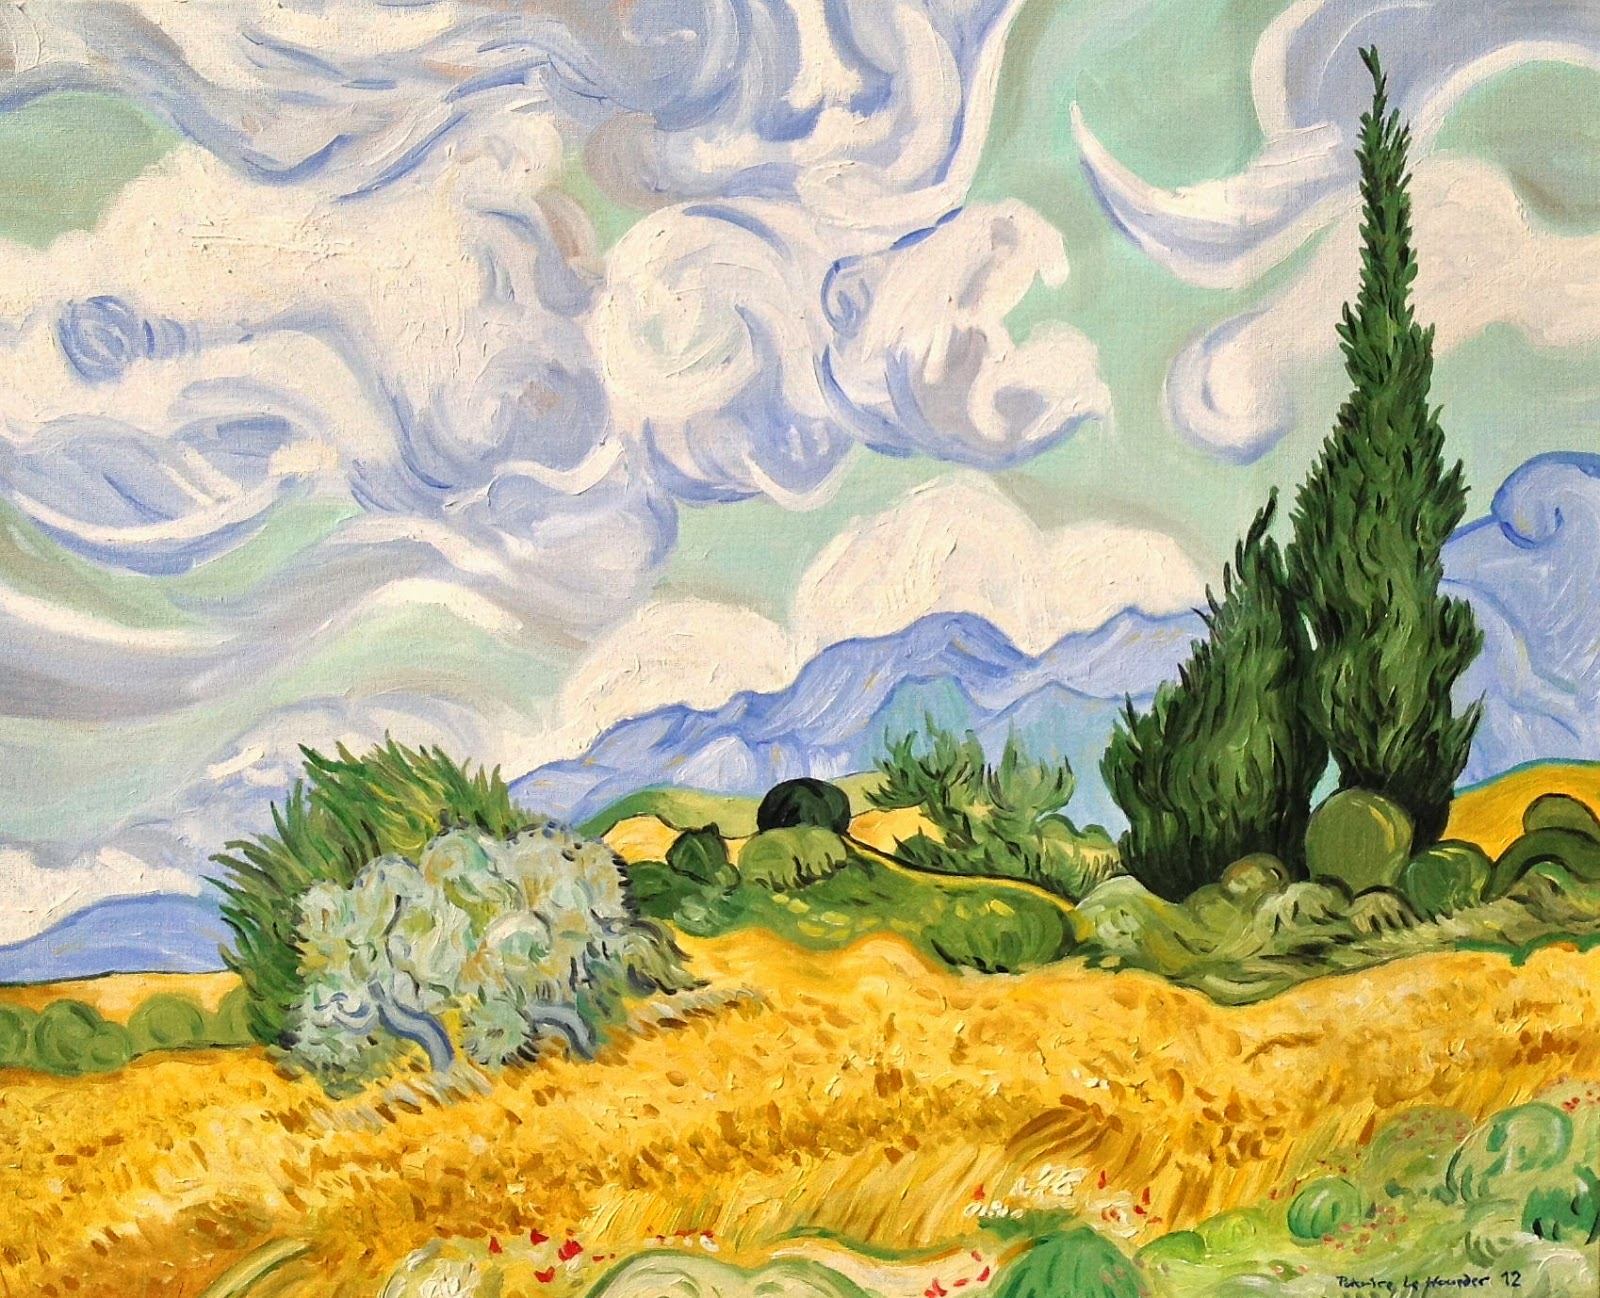
\includegraphics[scale=1.25]{v}}} % Image background
\centering
\vspace*{5cm}
\par\normalfont\fontsize{35}{35}\sffamily\selectfont
\textbf{PROGRAMMER L'INTERNET DES OBJETS }\\
{\LARGE }\par % Book title
\vspace*{1cm}
{\Huge Laurent TOUTAIN}\par % Author name
\endgroup

%----------------------------------------------------------------------------------------
%	COPYRIGHT PAGE
%----------------------------------------------------------------------------------------

\newpage
~\vfill
\thispagestyle{empty}

%\noindent Copyright \copyright\ 2014 Andrea Hidalgo\\ % Copyright notice

\noindent \textsc{IMT Atlantique}\\

\noindent Basé sur le MOOC PLIDO.\\ % License information

\noindent \textit{Publié le \today} % Printing/edition date

%----------------------------------------------------------------------------------------
%	TABLE OF CONTENTS
%----------------------------------------------------------------------------------------


\chapterimage{pano-5.jpg} % heading image

\pagestyle{empty} % No headers

\renewcommand\contentsname{Table des Matières}
\renewcommand{\bibname}{Bibliographie}
\tableofcontents% Print the table of contents itself

%\cleardoublepage % Forces the first chapter to start on an odd page so it's on the right

\pagestyle{fancy} % Print headers again

%----------------------------------------------------------------------------------------
%	CHAPTERS
%----------------------------------------------------------------------------------------
\chapter*{Acronymes}
\begin{multicols}{2}
\begin{acronym}
\acro{3GPP}{3rd Generation Partnership Project}
\acro{ABP}{Authentication By Personalisation}
\acro{ADSL}{Asymmetric Digital Subscriber Line}
\acro{AMQP}{Advanced Message Queuing Protocol}
\acro{AS}{Application Server}
\acro{ASCII}{American Standard Code for Information Interchange}
\acro{BLE}{Bluetooth Low Energy}
\acro{CBOR}{Concise Binaire Object Representation}
\acro{CoAP}{Constrained Application Protocol}
\acro{Cosem}{Companion Specification for Energy Management}
\acro{CRC}{Cyclic Redundancy Check}
\acro{CSV}{Comma Separated Values}
\acro{DLMS}{Device Language Message Specification}
\acro{DTT}{Digital Terrestrial Television}
\acro{DR}{Data Rate}
\acro{GSMA}{GSM Association}
\acro{HTML}{HyperText Markup Language}
\acro{HTTP}{HyperText Transport Protocol}
\acro{HTTPS}{HyperText Transport Protocol Secure}
\acro{IANA}{Internet Assigned Numbers Authority}
\acro{IBAN}{International Bank Account Number}
\acro{IEEE}{Institute of Electrical and Electronics Engineers}
\acro{IETF}{Internet Engineering Task Force}
\acro{IoT}{Internet of Things}
\acro{IP}{Internet Protocol}
\acro{IPv4}{Internet Protocol version 4}
\acro{IPv6}{Internet Protocol version 6}
\acro{IPSO}{IP for Smart Objects}
\acro{ITU}{International Telecommunication Union}
\acro{IRI}{International Resource Identifier}
\acro{ISBN}{International Standard Book Number}
\acro{ISO}{International Standardization Organization}
\acro{JMS}{Java Messaging Service}
\acro{JSON}{JavaScript Object Notation}
\acro{JSON-LD}{JavaScript Object Notation  for Linked Data}
\acro{LCIM}{Levels of Conceptual Interoperability Model}
\acro{LPWAN}{Low Power Wide Area Network}
\acro{LwM2M}{Lightweight Machine to Machine}
\acro{LNS}{LoRaWAN Network Server}
\acro{MQTT}{Message Queuing Telemetry Transport}
\acro{NAT}{Network Address Translation}
\acro{NGW}{Network GateWay}
\acro{NIDD}{Non IP Data Delivery}
\acro{OMA}{Open Mobile Alliance}
\acro{OTAA}{Over The Air Authentication}
\acro{OVH}{On Vous Herbèrge}
\acro{PAC}{Porting Authorization Code}
\acro{REST}{REpresentational State Transfer}
\acro{RFC}{Request For Comments}
\acro{RGW}{Radio GateWay}
\acro{RNIPP}{Répertoire National d'Identification des Personnes Physiques}
\acro{RSSI}{Received Signal Strength Indicator}
\acro{RTT}{Round Trip Time}
\acro{SCEF}{Service Capability Exposure Function}
\acro{SenML}{Sensor Measuring List}
\acro{SCHC}{Static Context Header Compression}
\acro{SF}{Spreading Factor}
\acro{SNR}{Signal to Noise Ratio}
\acro{SSID}{Service Set IDentifier}
\acro{STIC}{Sciences et Technologies de l’Information et de la Communication}
\acro{TCP}{Transmission Control Protocol}
\acro{TLV}{Type Length Value}
\acro{TNT}{Télévision Numérique Terrestre}
\acro{TTN}{The Things Network}
\acro{UDP}{User Datagram Protocol}
\acro{UIT}{Union internationale des télécommunications}
\acro{UNB}{Ultra Narrow-Band}
\acro{URI}{Universal Resource Identifier}
\acro{URL}{Univeral Resource Locator}
\acro{URN}{Univeral Resource Name}
\acro{VPS}{Virtual Private Server}
\acro{W3C}{World Wide Web Consortium}
\acro{WWW}{World Wide Web}
\acro{XML}{Extensible Markup Language}
\acro{XMPP}{Extensible Messaging Protocol et Presence}
\end{acronym}
\end{multicols}

%\chapterimage{pano-tv1.png} % Chapter heading image

\chapter{LES BASES DE L'INTERNET DES OBJETS (IOT)}

\section{Introduction}

  \vspace{1em}
 \begin{wrapfigure}{r}{2cm}
\Youtube{https://youtu.be/9edD2jEF3vM}
\end{wrapfigure}
 Dans cette première partie du cours, nous allons poser les bases de ce qu'est l'internet des objets (\ac{IoT} in english). Qu'est-ce qu'on entend par \ac{IoT} dans le cadre de livre~? Quelles sont les problématiques auxquelles doit répondre l'\ac{IoT} et son évolution aujourd'hui~? Quelles sont les technologies, les architectures, les protocoles sous-jacents qui seront utilisés dans cet ouvrage~? 
 
 Pour cela, nous allons faire un parallèle entre la manière dont l'internet a intégré la télévision et ce que l'on vit actuellement avec l'internet des objets. 
 
 \subsection{Réseaux dédiés}
   \vspace{1em}

\begin{wrapfigure}{r}{6cm}
\centerline{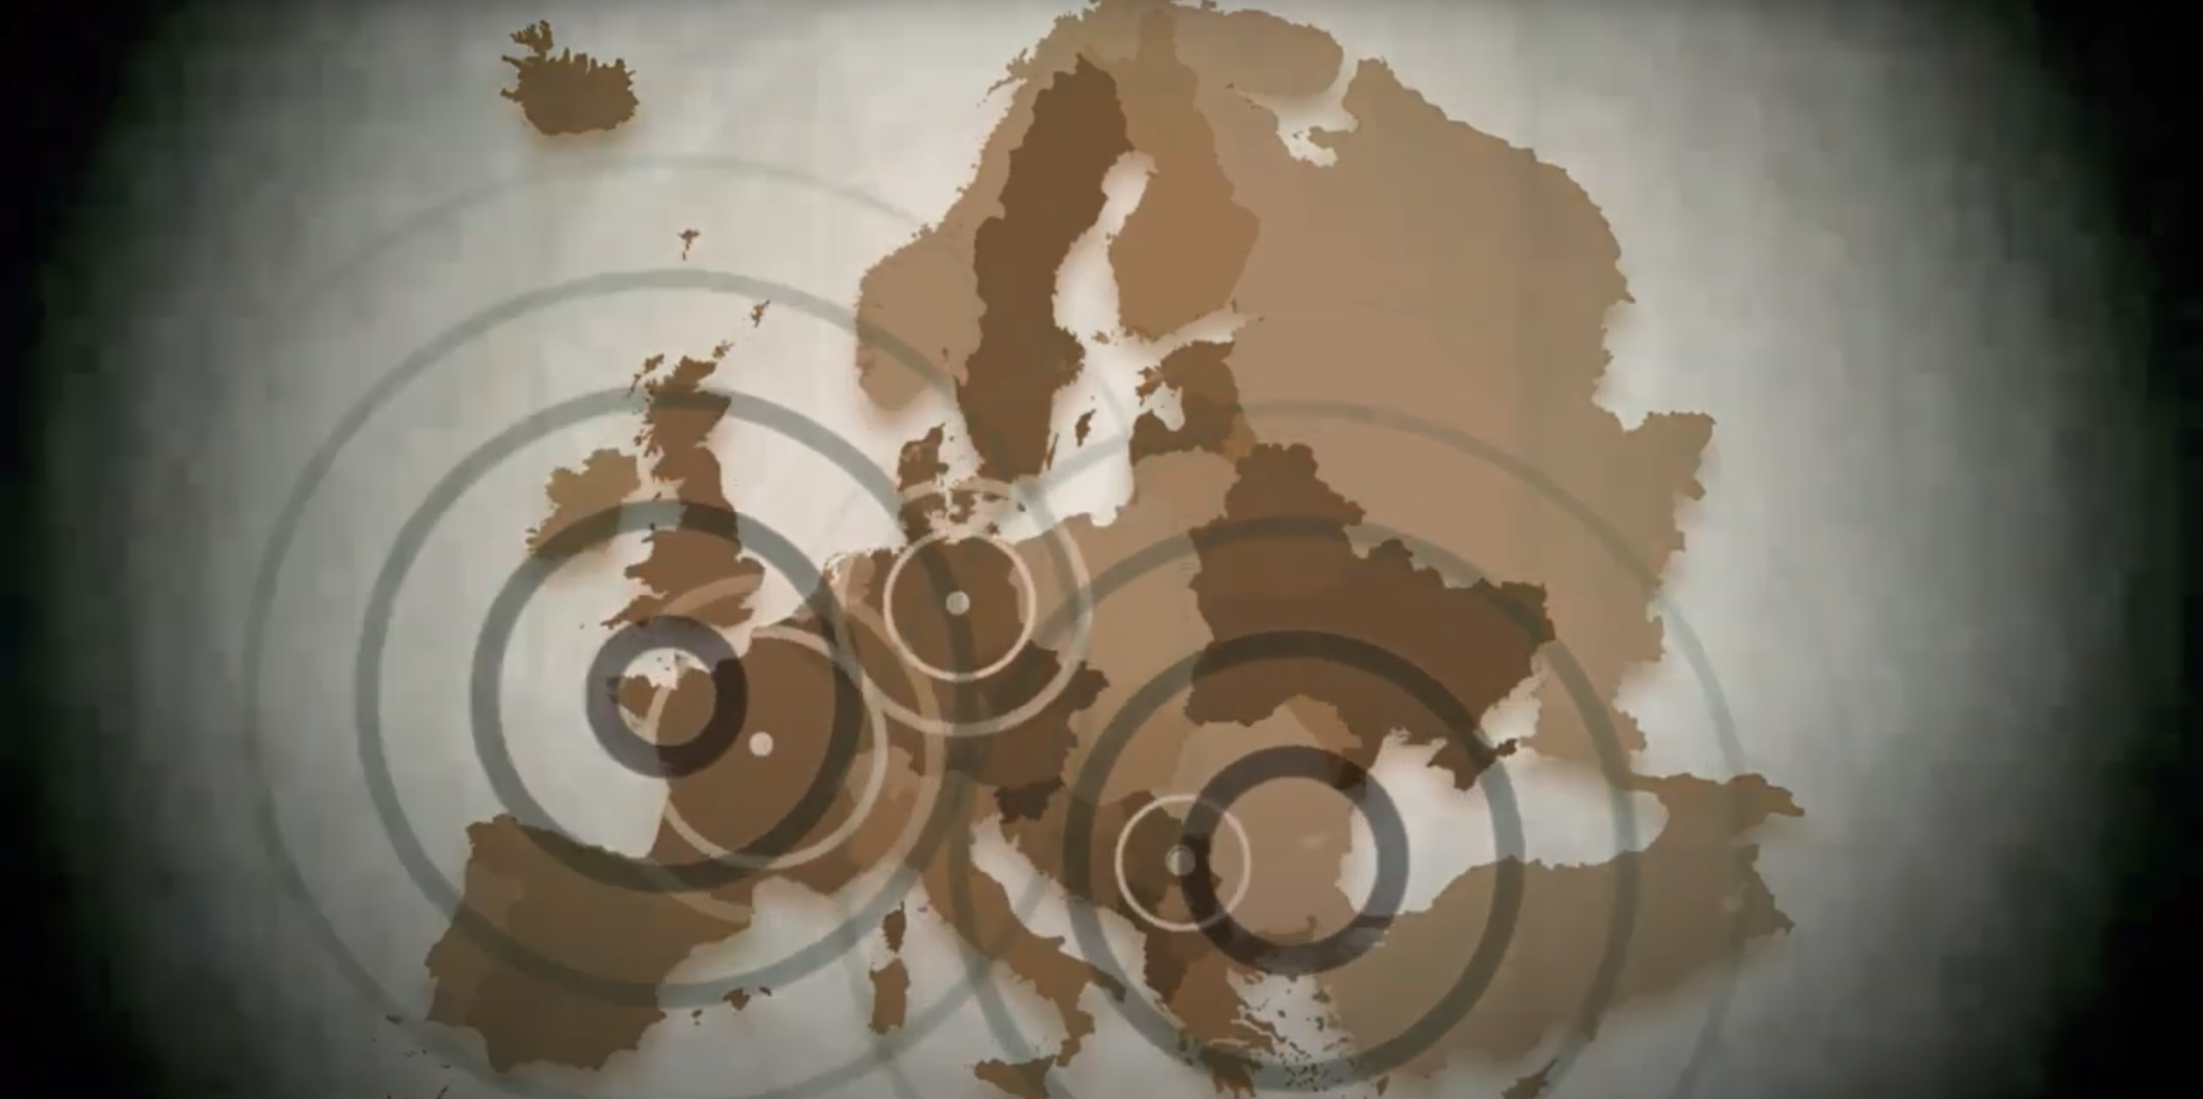
\includegraphics[width=.4\columnwidth]{Pictures/illu-propa.png}}
\end{wrapfigure}

 Dans les années 50, la télévision est devenue très populaire et presque tous les foyers ont acheté un téléviseur pour regarder leurs programmes préférés. Des réseaux de transmission dédiés ont été déployés partout sur la planète. En fait chaque type de communication avait son propre réseau un pour la radio un pour le téléphone un pour le télex,...
 


Dans les années 80, l'internet a vu le jour, mais les vitesses de transmission était faible et le réseau était limitée aux chargements de fichiers. Dans les années 90, des images et l'hypermédia avec le \ac{WWW} sont apparus, en lien avec l'augmentation des débits. Toujours dans les années 90, l'augmentation en puissance des microprocesseurs a permis la numérisation du signal télé. Les téléviseurs ont commencé à inclure des microprocesseurs et les réseaux sont passés d'une transmission analogique au numérique ; mais ils sont restés dédié à cet usage unique diffuser la télévision. Avec l'entrée dans le nouveau millénaire, l'internet a gagné en débit avec l'\ac{ADSL} et des fibres optiques. Il était possible d'intégrer des images dans les pages web mais la qualité était médiocre. Au même moment des centaines de canaux de télévision diffusaient en haute résolution leur programme via satellite ou par \ac{TNT}. De nos jours les communications internet ont gagné en vitesse et en qualité et certains pays ont coupé la \ac{TNT} et choisi de ne transmettre leurs programmes que par internet. En fait l'utilisation d'internet n'est pas uniquement un changement de réseau de distribution c'est aussi un changement majeur dans les usages et les applications. Vous pouvez regarder la télévision sur votre téléphone portable ou même regarder votre série favorite quand vous le voulez, à la demande. 

  \vspace{2em}

\subsection{3 phases technologiques}
   \vspace{1em}

\begin{wrapfigure}{r}{6cm}
\centerline{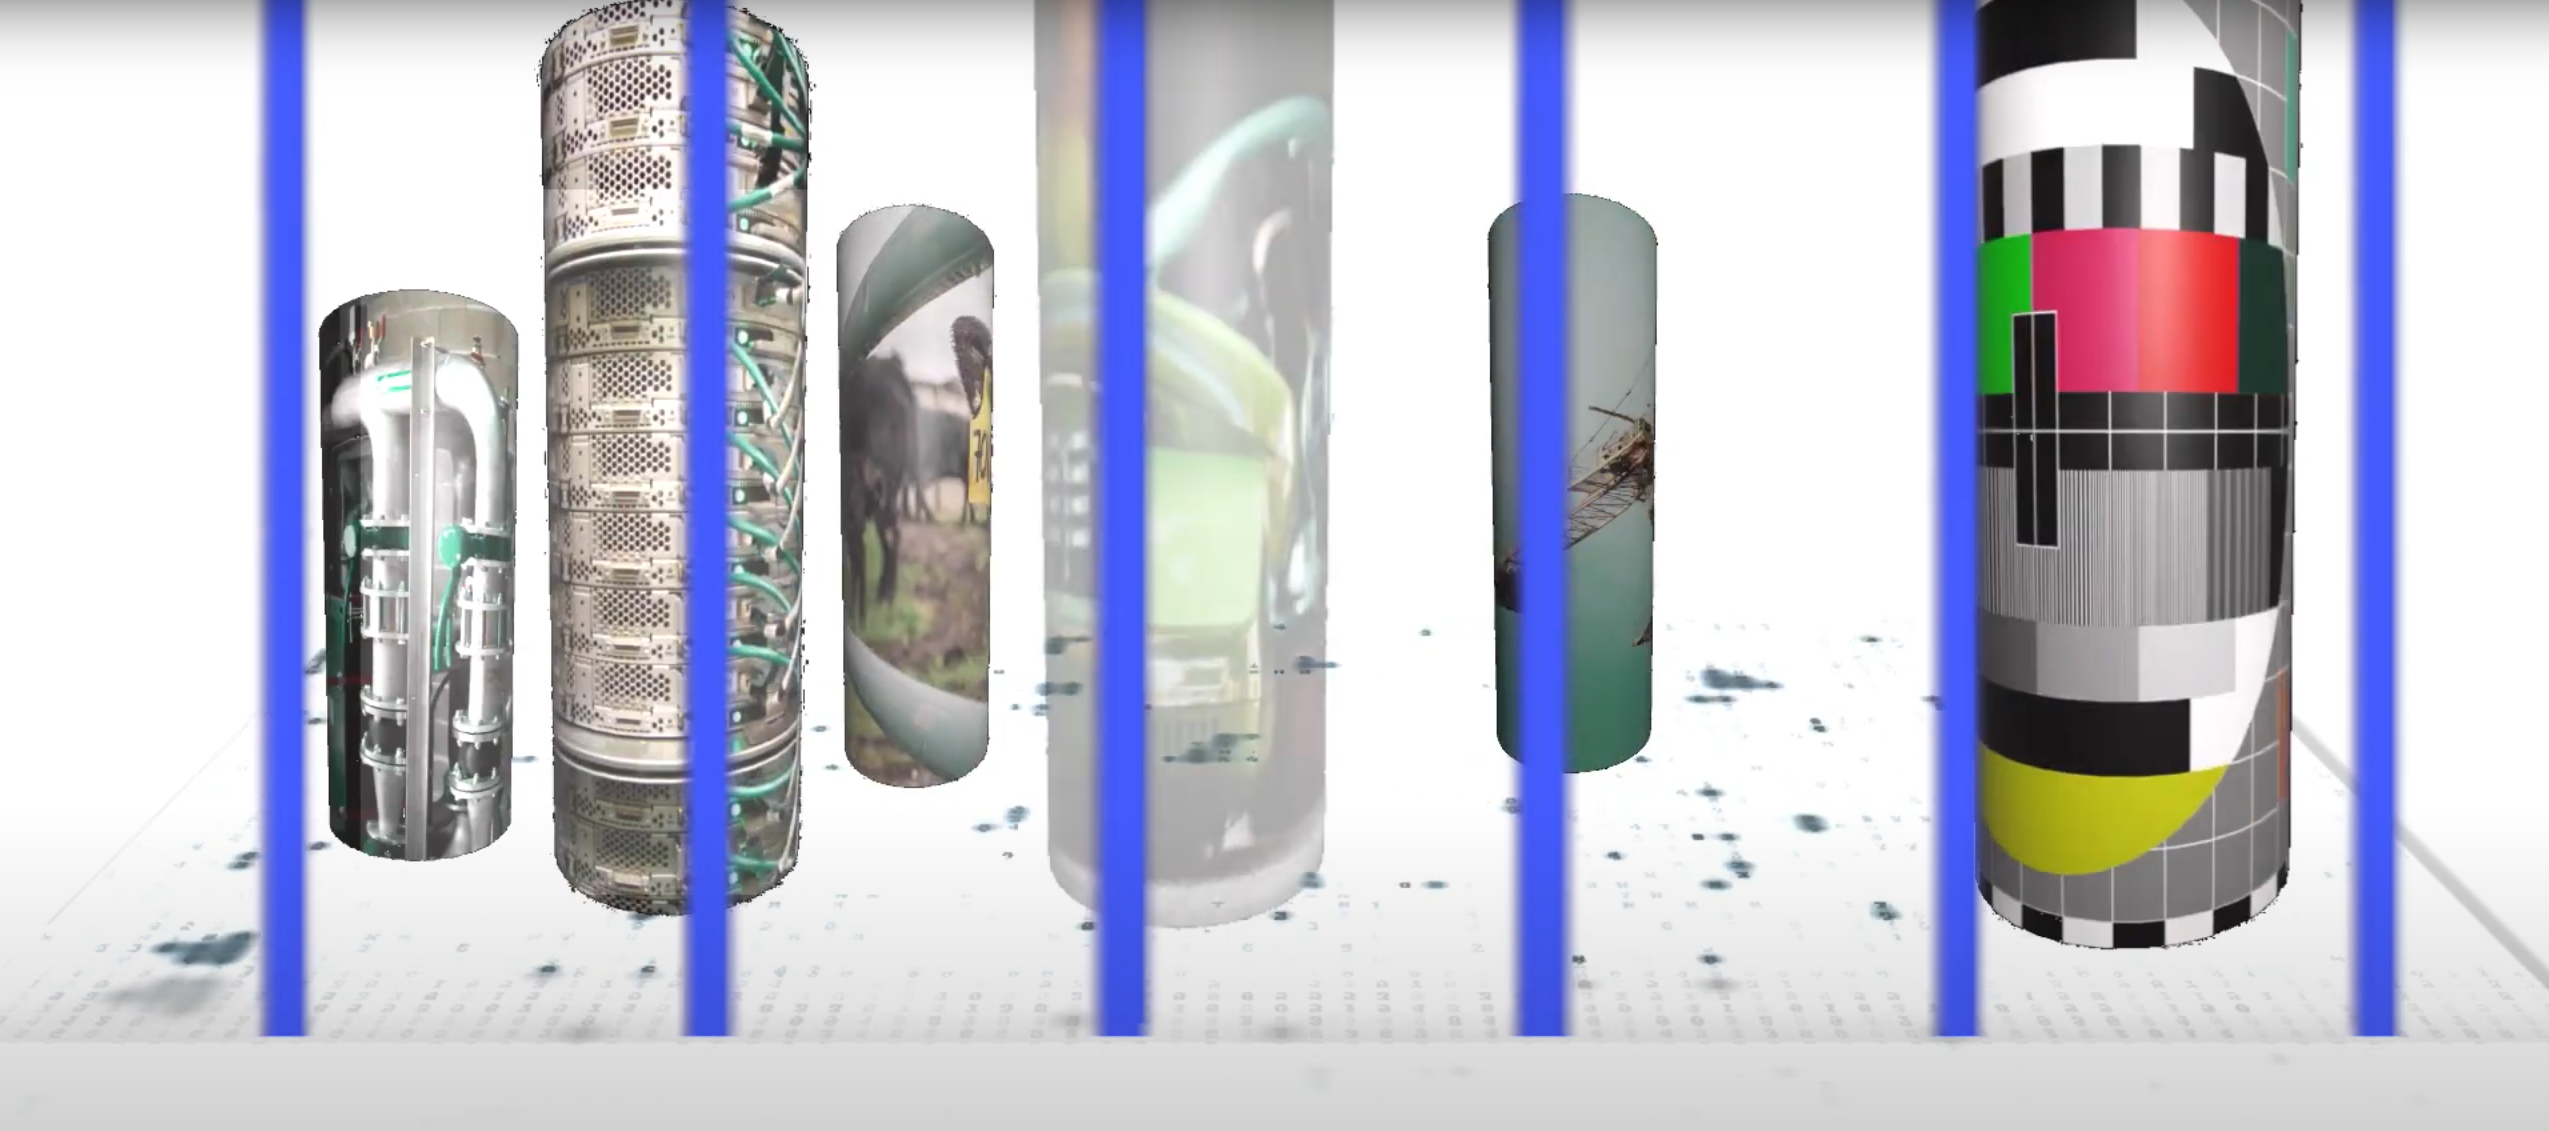
\includegraphics[width=.4\columnwidth]{Pictures/illu-verticals.png}}
\end{wrapfigure}
De cet exemple, on peut définir trois phases dans le développement d'une technologie. Dans la première phase, un réseau spécifique est construit pour un usage bien défini. On appelle cela une approche \Index{verticale} ; une technologie est dédiée à un seul usage. Il est difficile d'échanger de l'information entre deux verticales. On fait aussi référence à des \Index{silos} car ils sont isolés. Dans une seconde phase, les verticales commencent à intégrer des technologies communes mais pas d'une manière coordonnée. Elles ne peuvent toujours pas communiquer facilement car elles n'ont pas fait les mêmes choix.

~

\begin{wrapfigure}{r}{6cm}
\centerline{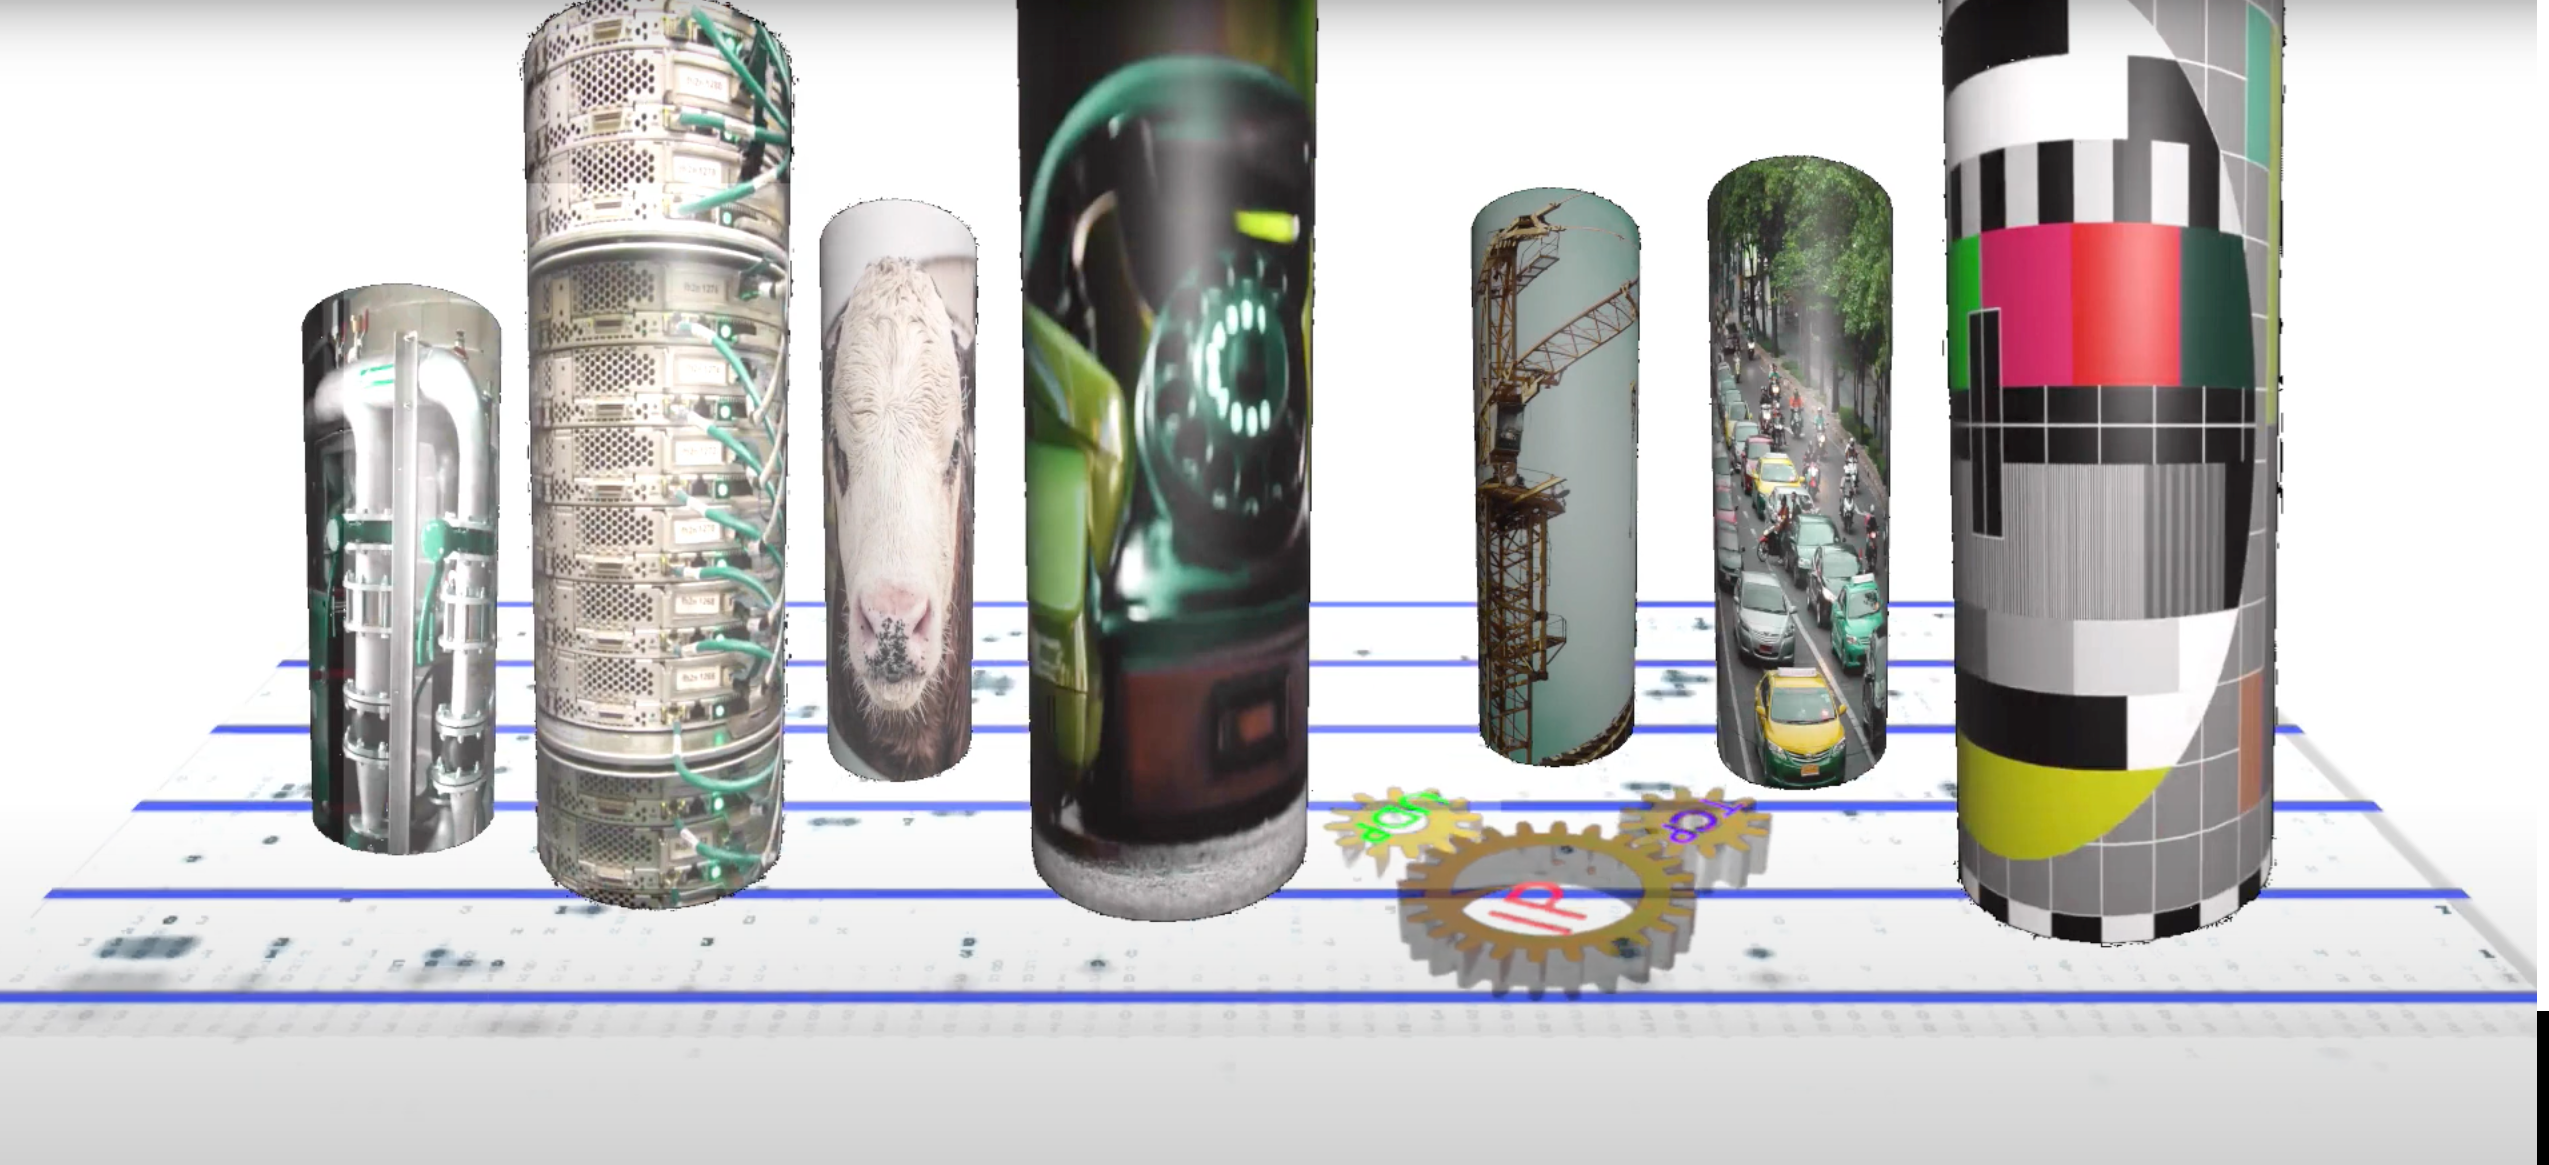
\includegraphics[width=.4\columnwidth]{Pictures/ill-horizontales.png}}
\end{wrapfigure}
Dans une dernière phase, des verticales se coordonnent pour converger vers les mêmes technologies en définissant des règles et des usages communs. Ceci dans le but de réduire les coûts ou d'augmenter leur impact dans ce cas. On parle d'horizontal\index{Horizontale} car elle couvre plusieurs secteurs. L'internet est devenu une de ces horizontales pour beaucoup de services. L'internet des objets suit ce même mouvement. Des solutions particulières ont émergé pour résoudre des besoins spécifiques en agriculture, dans l'automobile, dans la santé, dans l'énergie. Quand les réseaux internet ont permis des communications à faible coût, l'architecture de l'internet a été prise en compte mais sans compatibilité. Le changement qu'on vit actuellement est la définition de fonctionnalités communes à différents domaines. Le but étant de réduire les coûts mais également de croiser les informations pour une meilleure gestion du processus industriel et un meilleur usage des ressources
 

  \vspace{2em}

\section{L'Internet des Objets}

  \vspace{1em}
  
 Comment définir l’internet des objets~? Ou plutôt, quel internet des objets allons-nous étudier~? L’ambiguïté des deux termes "internet" et "objets" impose une définition plus précise ; ou du moins une classification pour mieux comprendre à quoi l’on fait référence.

  \vspace{1em}


L’internet est maintenant totalement intégré dans nos vies, pour le travail, l’enseignement, pour les distractions. On l’utilise à la maison ou au travail sur nos ordinateurs, et on l'emporte avec nous de plus en plus avec nos smartphones. 

Chacun a sa définition de ce qu’est internet. Pour le grand public, il peut s’agir d’applications très populaires comme Facebook, Tik-Tok, Netflix, Zoom. Pour certains, un peu plus technophiles, l’internet peut être confondu avec le Web auquel on accède via Chrome ou Firefox. Les techniciens parleront de protocoles comme IP, TCP, HTTP, et d’adresses comme les adresses IP ou les URL.

~~

Comme ce livre est orienté technologie, notre approche relève plutôt de cette dernière catégorie. Nous verrons comment des protocoles développés il y a une vingtaine d’années pour des ordinateurs peuvent s’appliquer à d’autres dispositifs qu’il nous reste à définir.

L'objectif de l'internet des objets est de poursuivre l'intégration du réseau Internet pour permettre à autre chose que des ordinateurs d'échanger des données. Le but principal est d'optimiser les processus pour qu'ils soient plus efficaces pour économiser des ressources ou d'augmenter la productivité. Il s'agit donc d'un internet enfoui, loin du frigo ou de la montre connectés, qui vont remonter des informations avec une infrastructure ou d'autres équipements. On peut imaginer des capteurs dans une usine pour contrôler la production, des voitures connectées qui vont dialoguer pour éviter les collisions, la mesure du taux de remplissage des bennes de recyclage dans une ville pour optimiser les circuits de collecte, la surveillance du degré d'humidité d'un champ pour réduire la consommation d'eau...


L’internet des objets peut se résumer de la manière suivante : utiliser des protocoles développés pour des ordinateurs et maintenant des téléphones portables (plus puissants que les ordinateurs utilisés par l’internet à ses débuts) mais dans des environnements plus contraints. En effet, les lois de Moore, définissant les puissances de traitement des processeurs ainsi que la diminution continue des coûts de la mémoire, nous ont permis de doter les petits objets de ressources comparables à celles des ordinateurs d’il y a trente ans.

L’internet des objets, c’est résoudre l’équation suivante : continuer à faire la même chose car tous les systèmes d’information actuels utilisent les mêmes principes mais le faire différemment car ces principes sont trop coûteux en énergie, en temps de calcul et échange de données.

L’\ac{IoT}, l’internet des objets ou des choses, est une architecture globale permettant à des objets (équipements de même type ou non), d’interagir de manière autonome via internet. Cette interaction :

\begin{itemize}
    \item est réalisée, par construction, au travers d’un réseau internet, ce qui implique généralement que les objets/choses soient pourvus d’une adresse IP ;
    \item est relatif à des commandes (opérations de contrôles ou appels de fonctions) ou des échanges de données ou d’informations.
\end{itemize}
est réalisée, par construction, au travers d’un réseau internet, ce qui implique généralement que les objets/choses soient pourvus d’une adresse IP ;
est relatif à des commandes (opérations de contrôles ou appels de fonctions) ou des échanges de données ou d’informations.
Ce nouveau paradigme \ac{STIC} qu’est l’IoT est une convergence de nombreux domaines d’applications tels que : les maisons ou bâtiments intelligents, les villes du futur, l’industrie du futur (industrie 4.0), l’énergie, les systèmes de transport, l’agriculture, la eSanté, etc., vers une suite protocolaire réduite, interopérable et sécurisée. Le mouvement est en marche et, vu le nombre d'acteurs concernés, va prendre plusieurs années. Mais les bases sont déjà bien établies et c'est ce que vous allez apprendre dans cet ouvrage.

 \vspace{2em}
 
\section{Le problème}

  \vspace{1em}

Un des problèmes que rencontre l’internet des objets, c’est que l’IoT ne démarre pas ex-nihilo. Maintenant que les technologies qui ont fait le succès de l'Internet sont matures, il ne s'agit pas juste de les appliquer à un nouveau domaine. Des objets étaient capables de communiquer bien avant qu’internet n’existe. Chaque secteur a déjà développé ses solutions, plus ou moins standards, plus ou moins propriétaires.

La figure~\vref{fig-bazar} reprend un certain nombre de travaux et de groupes qui spécifient les protocoles pour l’internet des objets. 

\begin{figure}[tbp]
\centerline{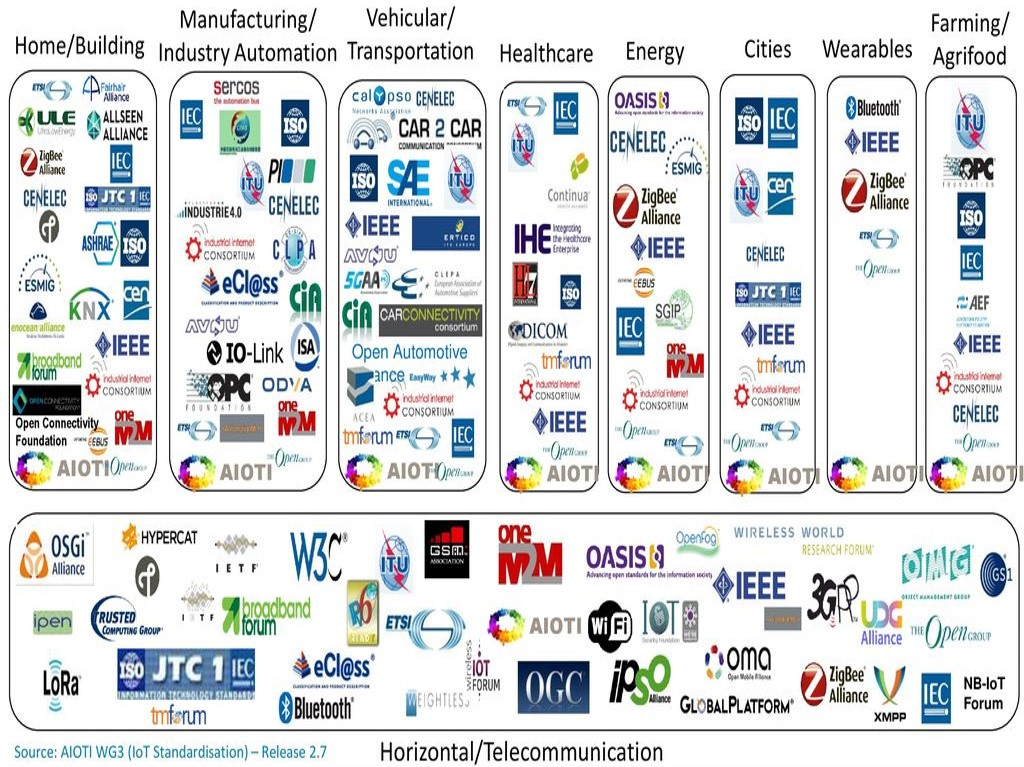
\includegraphics[width=1\columnwidth]{Pictures/IOTBazar_Domaines.jpeg}}
\caption{Quelques standards de l'IoT}
\label{fig-bazar}
\end{figure}

Sans entrer dans les détails, on voit que certains logos se retrouvent à plusieurs emplacements, qu’il y a pour chaque secteur une profusion de solutions qui nuisent à l’interopérabilité et aux évolutions. L’internet des objets, dans son acception la plus large, consiste à simplifier cette architecture, comme l’internet l'a fait il y a quelques années dans le domaine des télécoms en simplifiant ce modèle et en permettant à ces différents acteurs de converger vers une architecture commune et un ensemble de solutions plus réduit.

Cela ne veut pas nécessairement dire moins d’acteurs, mais une plus grande cohérence dans les choix technologiques.

La figure~\vref{fig-bazar-OS} analyse l’IoT par domaine d’application en se focalisant sur la composante réseau. L’IoT et les objets connectés sont des systèmes complexes pour lesquels les solutions open source, les alliances entre industriels, les organismes de standardisation sont toujours fragmentés ; cependant de manière moins importante, montrant que la structuration est en marche.

\begin{figure}[tbp]
\centerline{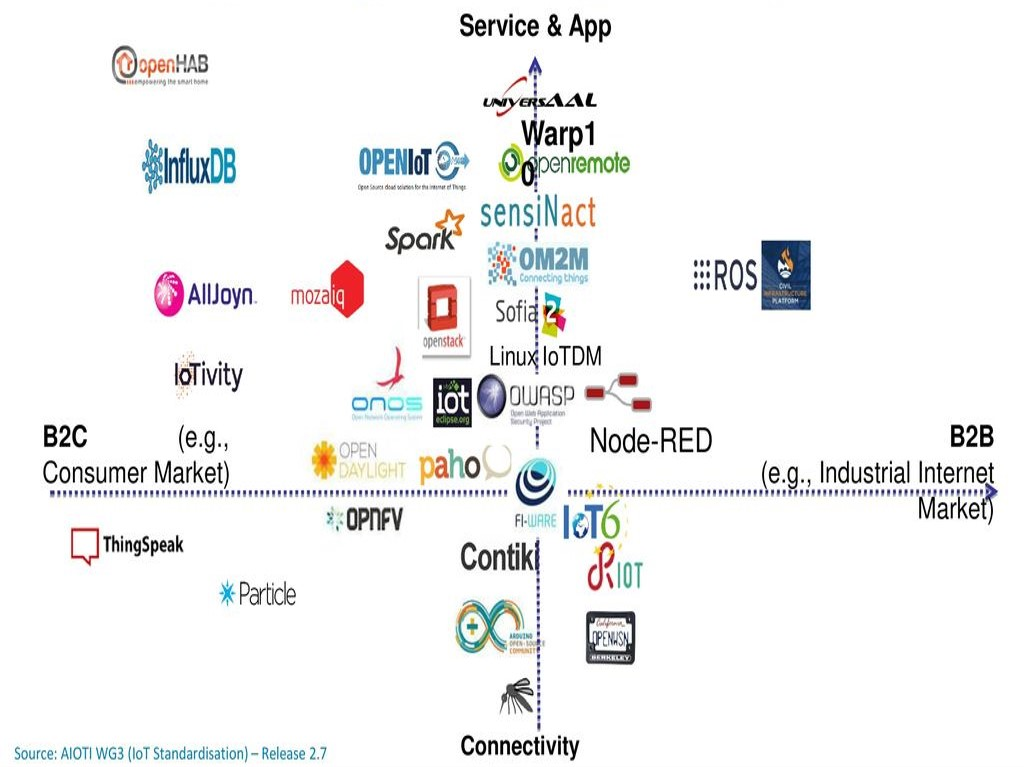
\includegraphics[width=1\columnwidth]{Pictures/IOTBazar_OpenSources.jpeg}}
\caption{Quelques applications Open Source pour l'IoT}
\label{fig-bazar-OS}
\end{figure}

Cette fragmentation de l’écosystème est paradoxale. Si l’on résume sommairement, les solutions proposées reviennent à interroger un équipement sur le terrain pour accéder à une valeur, la traiter et renvoyer une commande pour interagir avec l’environnement.

Pourquoi cette foison de solutions différentes~? Cela peut venir des besoins de fiabilité, de sécurité, de portée de la donnée, mais cela vient aussi de l’histoire. La communication avec des objets est tout aussi ancienne que la communication entre ordinateurs (qui sont eux-mêmes des objets). Mais à l’époque, chaque domaine a suivi sa propre voie en spécialisant les solutions pour répondre à ses besoins propres. Il en résulte des solutions optimisées pour un domaine particulier. Mais chaque fois qu’il faut modifier une technologie, le travail doit être adapté pour chaque domaine, introduisant des coûts et des délais supplémentaires.

De même, chaque domaine ayant sa propre représentation des données, il est relativement difficile de les combiner pour avoir une vision plus globale. On arrive donc à des systèmes fermés, chers, peu évolutifs, mais optimisés pour les tâches qu’ils ont à réaliser.

Au fil du temps, les protocoles de l’internet ont pu être utilisés, mais il s’agit surtout de complémenter les technologies existantes sans qu’il soit possible d’interconnecter deux domaines.


  \vspace{2em}

\section{Evolution de l'IoT}

  \vspace{1em}

L’exemple de l’évolution du réseau de télévision est éloquent. À ses débuts, ce réseau est analogique et hautement spécialisé pour diffuser les programmes transportés sur des signaux analogiques sur des équipements spécialisés, les téléviseurs.

Avec les progrès des processeurs informatiques, il devient possible de transporter les données en utilisant un codage numérique. Mais des réseaux spécialisés restent nécessaires, l’Internet n’offrant pas la même qualité.



La dernière étape consiste à intégrer ces flux dans l’internet classique. Cela devient possible par la montée en débit des réseaux filaires et radio (Wi-Fi, 4G...). 

Cette mutualisation des accès via l’internet permet non seulement une réduction des coûts, mais aussi l'apparition de nouveaux usages comme la télévision sur les téléphones portables ou les séries à la demande.

L’internet des objets suit la même voie. En plus des technologies spécifiques, les protocoles de l’internet sont intégrés, mais en les adaptant aux contextes du secteur.  Nous sommes actuellement en train de vivre la convergence vers un ensemble réduit de protocoles, une standardisation de la représentation de la donnée, et son traitement sur des plates-formes plus génériques. 

Le déclencheur n’est pas la montée en débit comme pour la télévision, mais la possibilité d'avoir des équipements peu chers, aux capacités réduites par rapport à l'informatique traditionnelle et autonomes énergétiquement, tout en ayant une meilleure intégration dans les systèmes d'information actuels.  

  \vspace{2em}

\section{Des objets contraints}

  \vspace{1em}

Avec les progrès de l’électronique, les processeurs deviennent de plus en plus puissants et les super-ordinateurs d’hier sont maintenant dans une montre ou un smart-phone. 

Pour l’internet des objets, la logique est un peu différente. La loi de Moore va induire une réduction des coûts de fabrication plutôt qu'une augmentation des puissances de traitement. Le principal critère pour un internet des objets massif reste l’énergie ; connecter un appareil à une source d’énergie ou recharger une batterie a un coût. Augmenter la vitesse du processeur ou la taille de la mémoire induit une plus grande consommation d’énergie de l'objet. On peut donc s’attendre à une certaine stabilité des performances des objets car ceux-ci resteront limités en performances.

Les objets sont généralement limités en termes de puissance de traitement, de mémoire et d’énergie. Selon le standard de l’IETF \rfc{7228}, les dispositifs peuvent être répartis en trois classes qui se retrouvent aussi dans la segmentation des processeurs :

\begin{itemize}
\item La classe 0, avec moins de 10 ko de mémoire volatile pour stocker les données temporaires et 100 ko de mémoire Flash pour stocker le code informatique de l'objet. C'est l’équivalent d’un Arduino UNO (2 ko de RAM et 32 ko de Flash). Il est presque impossible d’installer à la fois les protocoles utilisés pour communiquer sur Internet (même de manière restreinte) et les applications qui tournent dessus. 
\item La classe 1 a environ 10 Ko de RAM et 100 Ko de Flash. Avec une adaptation, il est possible d’y installer une pile IP. Il s'agit par exemple d'équipement comme le Pycom Lopy4 que nous utiliserons par la suite (et qui se situe dans la limite haute) sur lequel le système d'exploitation est minimal. Ainsi, le Pycom utilise une version simplifiée du langage Python (micro-python) qui permet de l'adapter à la limitation du système.
\item La classe 2 est moins restreinte avec au moins 50 ko de RAM et 250 ko de Flash (comme un Raspberry Pi). Le système d’exploitation Linux peut fonctionner sur ces appareils. Par conséquent, il y a peu de limitations sur la pile IP et les applications s’y exécutant.
Les appareils de classe 1 ont trop de restrictions pour utiliser les protocoles définis pour des objets plus gros. L’\ac{IETF}, l'organisme qui standardise les protocoles de l'internet, a proposé une révision de sa pile de protocoles afin d’adapter sa pile protocolaire à un environnement contraint.
\end{itemize}


La figure~\vref{fig-encap} résume les moyens d'interconnexion suivant la classe de l'objet~:
Un appareil de classe 0 ne peut pas utiliser directement l’internet pour échanger des informations, d’où la nécessité d’installer une passerelle pour capter le trafic et l’envoyer sur l’internet. Il ne possède pas directement d'adresse IP. Les passerelles LoRaWAN \ac{LNS} et \acs{3GPP} \ac{SCEF} agissent dans ce sens (nous reviendrons là-dessus). Les données produites sont encapsulées par ces passerelles dans des protocoles comme \ac{HTTP} ou \ac{MQTT}, que nous verrons également dans la suite du cours.

Les appareils de classe 1 peuvent aussi utiliser une passerelle pour s’interconnecter à l’internet traditionnel, mais plutôt que d'encapsuler les données produites dans d'autres protocoles comme le fait la classe 0, les passerelles pour les appareils de classe 1 vont traduire un protocole contraint dans son équivalent dans le monde non contraint.

Les dispositifs de classe 2 peuvent interagir directement avec d’autres nœuds sur l’internet, sans passer par une passerelle.

\begin{figure}[tbp]
\centerline{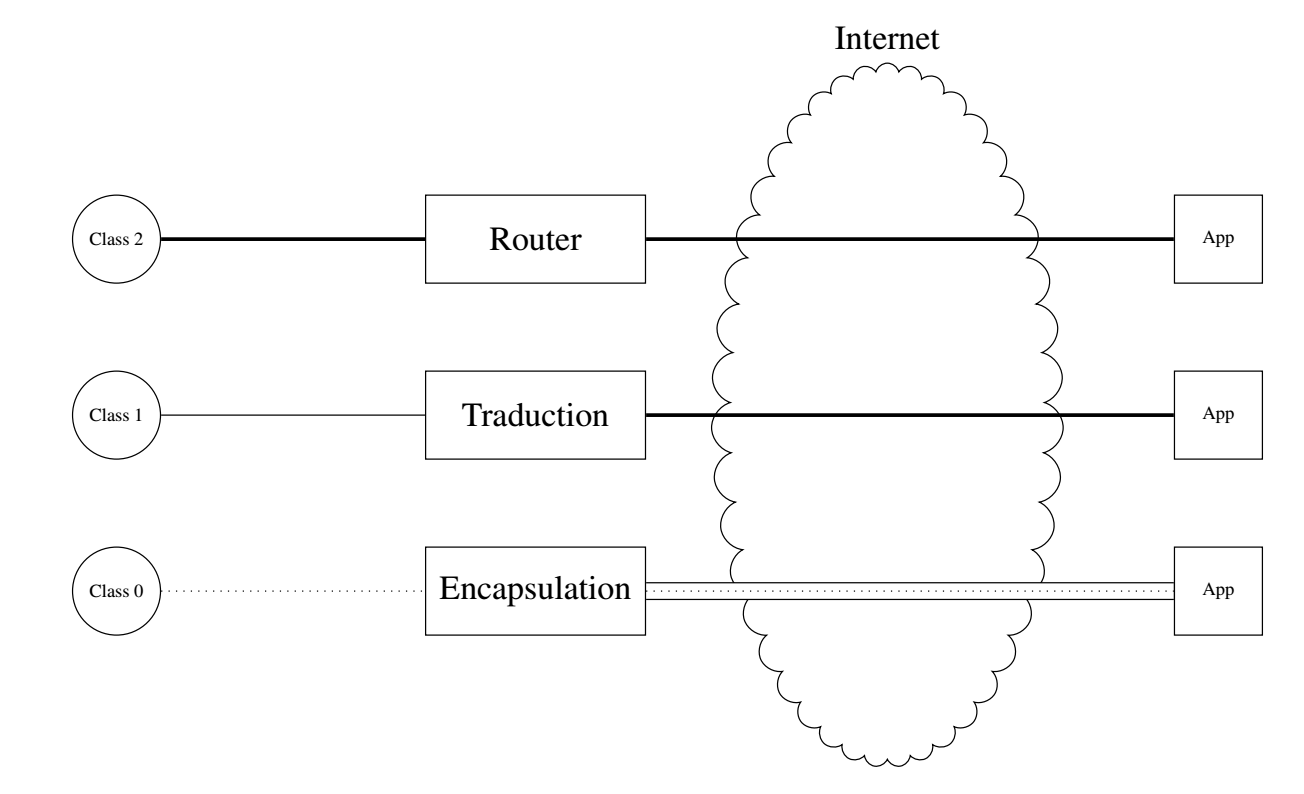
\includegraphics[width=1\columnwidth]{Pictures/Encpasul.png}}
\caption{Possibilités d'interconnection}
\label{fig-encap}
\end{figure}

  \vspace{2em}

\section{L'interopérabilité}

  \vspace{1em}

Un autre défi concerne le nombre de dispositifs. Certaines études prévoient 500 milliards de dispositifs à la fin de la décennie.

Avec cet énorme internet des objets, où presque chaque équipement comprendra des éléments de détection ou d’action, l’intégration dans un système d’information deviendra un véritable défi. Comme l’internet des objets actuel est conçu pour une verticale (c'est-à-dire pour des applications spécifiques), les dispositifs sont choisis et intégrés au moment de la conception du système. Les ingénieurs choisissent leurs capteurs, connaissent précisément leurs caractéristiques et écrivent leur code en fonction de ce qu'ils ont intégré. 

L’internet des objets massif change la donne. Les dispositifs ou les choses ne peuvent pas être intégrés dès le départ dans un système d’information statique. L’intégration doit se faire au fil du temps et doit gérer les évolutions des dispositifs pendant longtemps (les fabricants de dispositifs peuvent changer, les produits évolueront avec de nouvelles fonctionnalités, etc.)

Cette question d’interopérabilité a été formalisée dans le modèle \ac{LCIM}~\cite{tolk2003levels} (voir figure~\vref{fig-lcim}) peut être représenté par un compteur pour mesurer le degré d'interopérabilité.

\begin{figure}[tbp]
\centerline{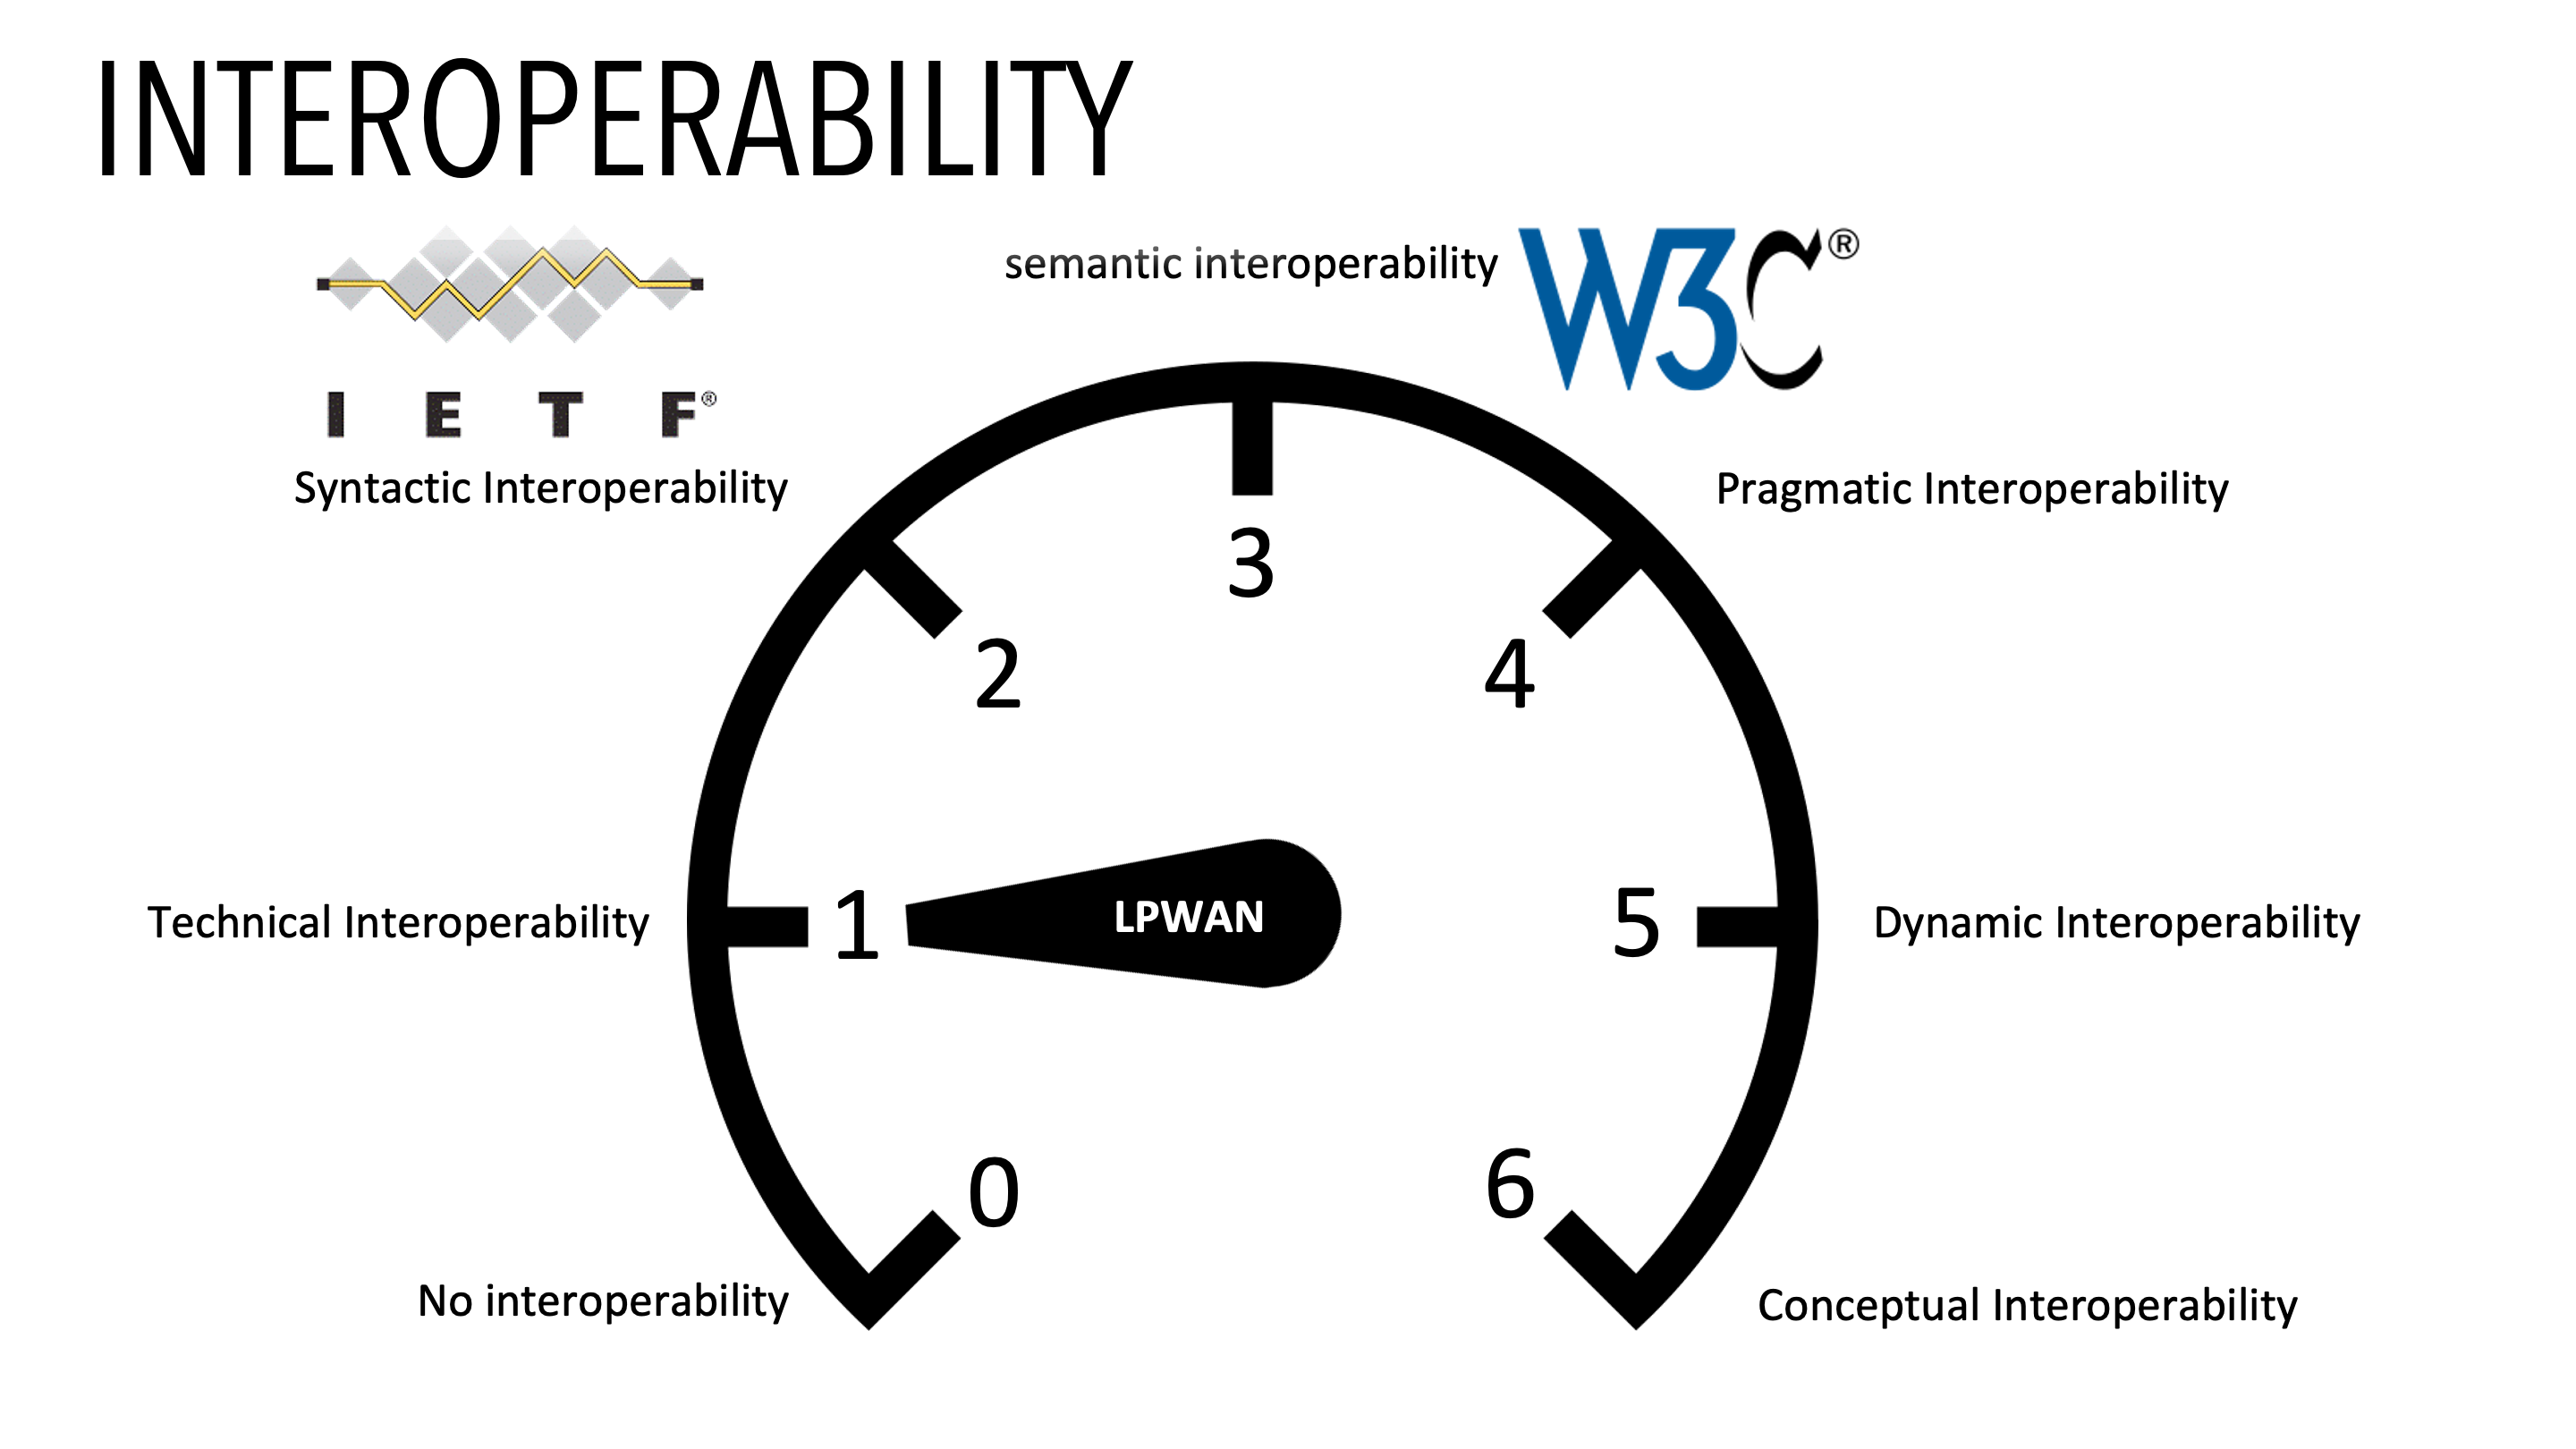
\includegraphics[width=1\columnwidth]{Pictures/TPT2020.png}}
\caption{Niveau d'interopérabilité}
\label{fig-lcim}
\end{figure}


Il distingue six niveaux d’interopérabilité, parmi lesquels :

\begin{itemize}
     \item Au niveau zéro, on n'est pas connecté ; on ne parle à personne donc on n'a pas de problèmes d'interopérabilité. 
    \item  Au niveau 1, on est capable de transmettre de l'information,  mais il faut que les deux côtés connaissent les règles. On a un système intégré ; les applications doivent  connaître précisément les spécifications des objets avec lesquels ils communiquent,  car elles définissent ses propres formats des échanges de données. On pourrait prendre l'exemple qu'une carte électrique où un processeur communique avec des capteurs via un circuit imprimé. Le code tournant sur le processeur peut être écrit à l'avance car il y a peu de chance qu'un utilisateur dessoude les composants pour les remplacer par d'autres. Cela correspond à l'encapsulation, si l'on considère les objets en réseau de la figure~\vref{fig-encap}, l'élément d'interconnexion doit être configuré pour en fonction de l'objet émetteur encapsuler les données vers la bonne application chez le bon récepteur. 
    \item L’interopérabilité syntaxique (niveau 2) où deux nœuds peuvent échanger des données, sans être a préalable configurés pour cet échange. C'est le cas de l'Internet. En utilisant cette suite de protocoles, en ayant une adresse valide sur le réseau, toute application est capable d'échanger des données avec une autre. En revanche, les données que vous allez échanger sont propres à une application. Les vidéoconférences sont un très bon exemple d'interopérabilité de niveau 2. Vous ne pouvez pas utiliser Zoom si votre correspondant utilise Teams car les formats sont différents. L'\ac{IETF}  est le regroupement de différents acteurs (industriels, académiques,...) qui produisent les standards liés à ce réseau. Il se reconnaissent par l'acronyme \ac{RFC} suivi d'un nombre. 
    \item L’interopérabilité sémantique (niveau 3) implique que le récepteur est capable d'interpréter les données reçues.Le web est un très bon exemple d'interopérabilité de niveau 3. Quel que soit votre navigateur, vous pouvez afficher les pages d'un site web et suivre les liens. Le sens de l'information est compris de la même manière des deux côtés. Pour le Web, le format \ac{HTML} permet à l'aide de balises (mots-clés) de structurer un texte en y ajoutant des informations de formatage ou des liens vers d'autres documents. Le W3C définit les standards.
     \item Les niveaux supérieurs d'interopérabilité vont être lié à la précision du modèle qui va représenter le système.     
\end{itemize}


L'internet qu'on connaît est une très bonne illustration du besoin d'interopérabilite. Il a permis, grace à une uniformisation du réseau et une force baisse des coûts de transmission, de développer de nouveaux usages. Vous n'auriez jamais investi pour un réseau propre à la vidéoconférence et au télétravail. Mais en mutualisant les usages, c'est possible ! L'internet des objets doit suivre la même voie et également converger vers l'architecture de l'internet actuel. Le mot clé est donc l'interopérabilité.  
   \vspace{2em}

\section{Le besoin de standardisation}
  \vspace{1em}

Les objets n'ont pas attendu l'internet pour communiquer. Ils ont évolué chacun dans leur verticale, développant des solutions satisfaisantes mais limitées en termes d'évolution et d'interopérabilité. Cet état des lieux sur la dispersion des écosystèmes met en avant la nécessité :

\begin{itemize}
\item d’une coordination entre les alliances ;
\item d’une harmonisation ou d’un alignement des standards ;
\item de disposer au plus vite d’implémentations de référence et de modèles de référence.
\end{itemize}

Dans le cas contraire, l’interopérabilité ne pourra pas être traitée comme il se doit, les nouveaux services innovants multi-domaines ne seront pas couverts, et le développement de l’IoT pourrait être freiné voire avorté.

Les aspects liés à l’éducation et à la formation des acteurs de l’IoT, ainsi que ceux liés à l’acceptation, aux usages et évidemment au volet socio-économique de l’IoT, sont aussi des points essentiels dont il faut tenir compte.

Les organismes de normalisation tels que l’\ac{IETF} ou le \ac{W3C} ont conçu des protocoles ou des modèles de données capables de traiter l’interopérabilité. D’une certaine manière, c’est la clé du succès de l’internet actuel. Il a permis de résoudre le problème de l’interopérabilité au niveau syntaxique et sémantique mais au prix de messages volumineux.

Le défi pour l’internet des objets est de s’intégrer dans ce système distribué géant. Comme l’internet des objets est un nouveau venu, l’évolution devra se faire de son côté pour prendre en compte les règles existantes, mais en les adaptant. Les prochains chapitres traiteront de ces changements.

\section{Questions}

\Question{Nouveau Domaine}{Les objets communicants sont un tout nouveau domaine, lié aux progrès en miniaturisation des composants électroniques:
\begin{itemize}[label=$\circ$]
\item \Wrong{Vrai}
\item \Correct{Faux}
\end{itemize}
 }{Les objets communicants ont toujours existé, même avant le déploiement des protocoles de l'Internet. Ce qui est nouveau c'est leur intégration dans les architectures Internet actuelle pour mieux traiter l'information qu'ils produisent.
 }
 
 \Question{Protocoles}{Laquelle de ces affirmations est vraie ?
\begin{itemize}[label=$\circ$]
\item \Wrong{Il y a très peu de protocoles pour faire communiquer les Objets. Comme l'Internet est une technologie qui s'est très répondue, son succès va permettre aux objets de communiquer.}
\item \Correct{ Il y a beaucoup de solutions pour permettre à des objets de communiquer, l'Internet des Objets doit permettre de les fédérer.}
\end{itemize}
 }{Chaque métier a créé ses propres protocoles.}
 
 
\Question{Source de données}{Quelle est la principale source de création des données dans l'IoT ?
\begin{itemize}[label=$\circ$]
\item \Correct{les capteurs}
\item \Wrong{les nano-ordinateurs (type Raspberry Pi)}
\item \Wrong{Internet}
\item \Wrong{les serveurs Web}

\end{itemize}
 }{Les mesures effectuées par les capteurs constituent la principale source de création des données de l'IoT.}

\Question{Défis}{Quels sont les principaux défis technologiques pour l'Internet des Objets (3 réponses) ?
\begin{itemize}[label=$\square$]
\item \Correct{Avoir une consommation d'énergie faible.}
\item \Correct{Avoir une architecture protocolaire simplifiée.}
\item \Wrong{Pouvoir fonctionner sur des systèmes d'exploitation ouverts comme Linux.}
\item \Correct{Permettre de sécuriser les données qui peuvent être sensibles }
\item \Wrong{Transmettre en permanence leur état et des valeurs mesurées.}

\end{itemize}
 }{les objets sont généralement contraints en énergie et en capacité. Pour limiter la consommation d'énergie, il ne faut pas émettre ou recevoir tout le temps, donc la transmission en permanence des données ne va pas dans ce sens. De même, un système d'exploitation comme Linux apparait surdimensionné.}
 
%%----------------------------------------------------------------------------------------
%	CHAPTER 3
%----------------------------------------------------------------------------------------

\chapterimage{pano-tv1.png} % Chapter heading image
\acresetall
\chapter{ARCHITECTURE DE L'INTERNET}

\section{Les protocoles}
  
    \vspace{1em}

  \begin{wrapfigure}{r}{8.5cm}
\centerline{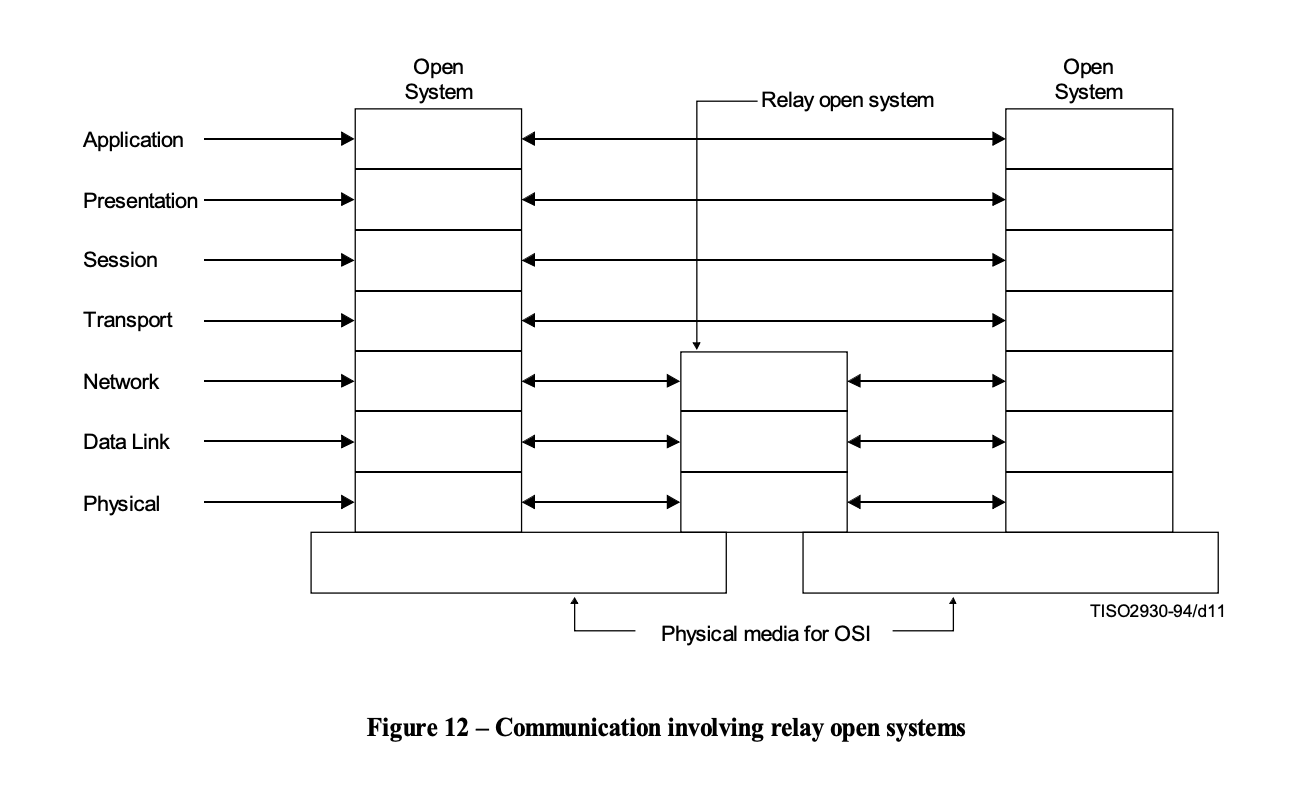
\includegraphics[width=.6\columnwidth]{Pictures/OSI.png}}
\caption{Extrait du standard ITU-T Rec. X.200 (1994 E)}
\end{wrapfigure}

Vous connaissez sûrement le principe d'empilement protocolaire dans les réseaux. Chaque protocole fournit un service et se base sur celui de la couche inférieure pour le réaliser. Le modèle d'origine définit sept couches pour transporter les données d'une application, n'importe où dans le monde.
  Les protocoles réseaux sont empilés les uns sur les autres, ceux du dessus utilisent les services offerts par ceux d’en dessous pour acheminer la donnée. Cela a donné lieu au modèle de référence de l’\ac{ISO} qui structure les réseaux depuis les années 1970. En théorie, il y a 7 \Index{couches}, mais l'internet a fait évoluer ce modèle et les numéros des couches, associés à des fonctionnalités, sont restés ; ce qui peut conduire à une numérotation étrange.
  
 \begin{figure}[tbp]
\centerline{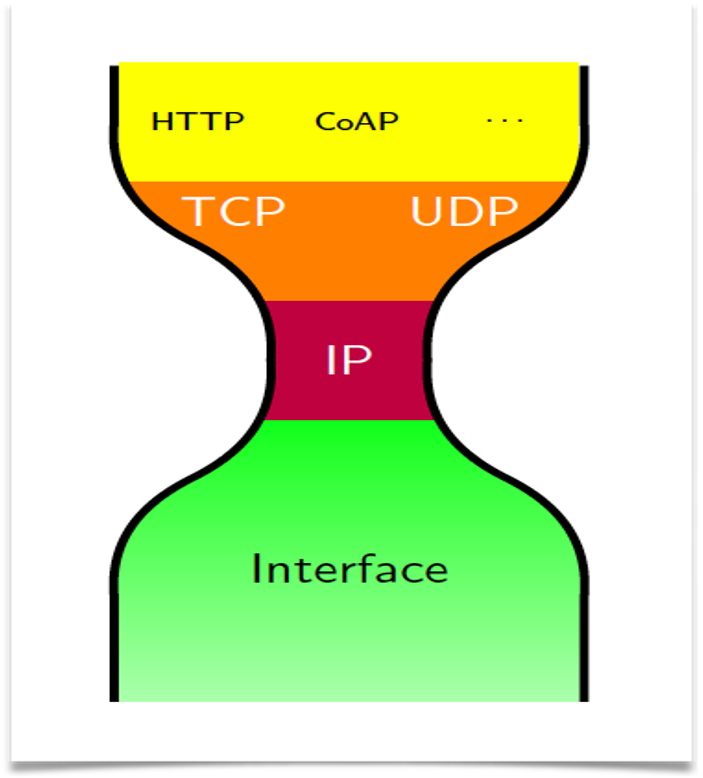
\includegraphics[width=.5\columnwidth]{Pictures/hourglass.png}}
\caption{Empilement protocolaire de l'Internet}
\label{fig-hourglass}
\end{figure}

  \vspace{1em}

\begin{wrapfigure}{r}{3cm}
\Youtube{https://youtu.be/vQ7zMVrqHbA}
\end{wrapfigure}

  L'internet a simplifié cette architecture (cf. figure~\vref{fig-hourglass}). C'est pour ça que l'on retrouve moins de couches et que les numéros ne sont pas contigus. 
  
  
    \vspace{1em}

  Les deux premières couches  en partant du bas, regroupées sous le nom d'Interface, permettent de transmettre les données binaires sur un support physique. La couche 1 s’occupe de cette modulation sur un support physique particulier (fibre optique, paire de cuivre, onde radio). La couche 2 regroupe les mécanismes qui permettent de structurer cette donnée sous forme de bloc de taille finie appelées trames, de définir les méthodes d’accès, c’est-à-dire quand l’équipement peut émettre, et les formats des adresses utilisées pour identifier les équipements. Ethernet ou Wi-Fi sont des exemples de protocoles de niveau 2 (qui intègrent leur niveau 1).

\begin{itemize}
\item l’\ac{IEEE} qui propose des standards comme Ethernet pour les réseaux filaires ou Bluetooth et Wifi pour les réseaux radio,
\item le \ac{3GPP}  qui opère au même niveau et définit les protocoles pour la téléphonie cellulaire (4G),
\item \ldots
\end{itemize}

  
    \vspace{1em}

  
  
  Au-dessus, on a le protocole \ac{IP} standardisé par l'IETF.  Le protocole \ac{IP} s’adapte simplement à tout moyen de communication. \ac{IP} propose ainsi une abstraction des moyens de communication aux couches applicatives, rendant l’accès au réseau et l’adressage universels. Le traitement dans les \Index{routeur}s (équipements chargés d’aiguiller l’information dans le réseau) doit être le plus rapide possible pour traiter un maximum de paquets par seconde. De plus, \ac{IP} ne spécialise pas le réseau pour un service ou un autre ; il ne fait qu’aiguiller les paquets vers la bonne destination. Le réseau Internet est un réseau mondial construit autour de ce protocole permettant potentiellement d'atteindre tous les équipements qui y sont connectés. 
  
  
  Les experts de l'internet aiment cette représentation en \Index{sablier} où \ac{IP} apparaît en position centrale mais est plus petit comparé aux autres protocoles. Par conception, \ac{IP} est très simple ; à la fois pour être portés facilement sur de nombreux niveaux 2 et être facilement utilisable par les couches hautes, mais également pour traiter les données très rapidement dans les nœuds d'interconnexion. 
  
  \ac{IP} est mis en oeuvre partout sur Internet aussi bien dans les équipements en extrémité du réseau que dans les routeurs chargés d'envoyer les données vers la bonne destination.
  
  
    \vspace{1em}

  Au-dessus on trouve deux protocoles qui ne sont mis en oeuvre que dans les équipements d'extrémité.  Si le niveau 3 permet de joindre une machine, le niveau 4 va permettre d’identifier l'application qui doit traiter les données. Les "adresses" de ces applications sont des numéros compris entre 1 et 65535 appelés \Index{port}s. Par exemple, les serveurs Web utilisent le port numéro 80 ou le numéro 443. 
  
  
  Le protocole \ac{TCP} va surveiller les données transférées et sera capable de retransmettre des données perdues, ralentir ou accélérer le transfert de données s’il détecte une saturation du réseau. En revanche, sa mise en œuvre est complexe et coûteuse en mémoire. Dans les cas simple, \ac{UDP} est préféré ; il n'apporte pas de traitement supplémentaire \ac{UDP}, c'est un protocole minimal qui se contentent d'aiguiller les données vers la bonne application sans aucun autre contrôle.
  

    \vspace{1em}

  
  Au-dessus, on trouve les applications qu'historiquement on classe dans la couche 7. Les applications sont très nombreuses mais la plus répandue est \ac{HTTP} qui sert à transporter les pages web, mais également elle permet des communications directes entre ordinateurs. 
  
  
    \vspace{1em}


   \begin{figure}[tbp]
\centerline{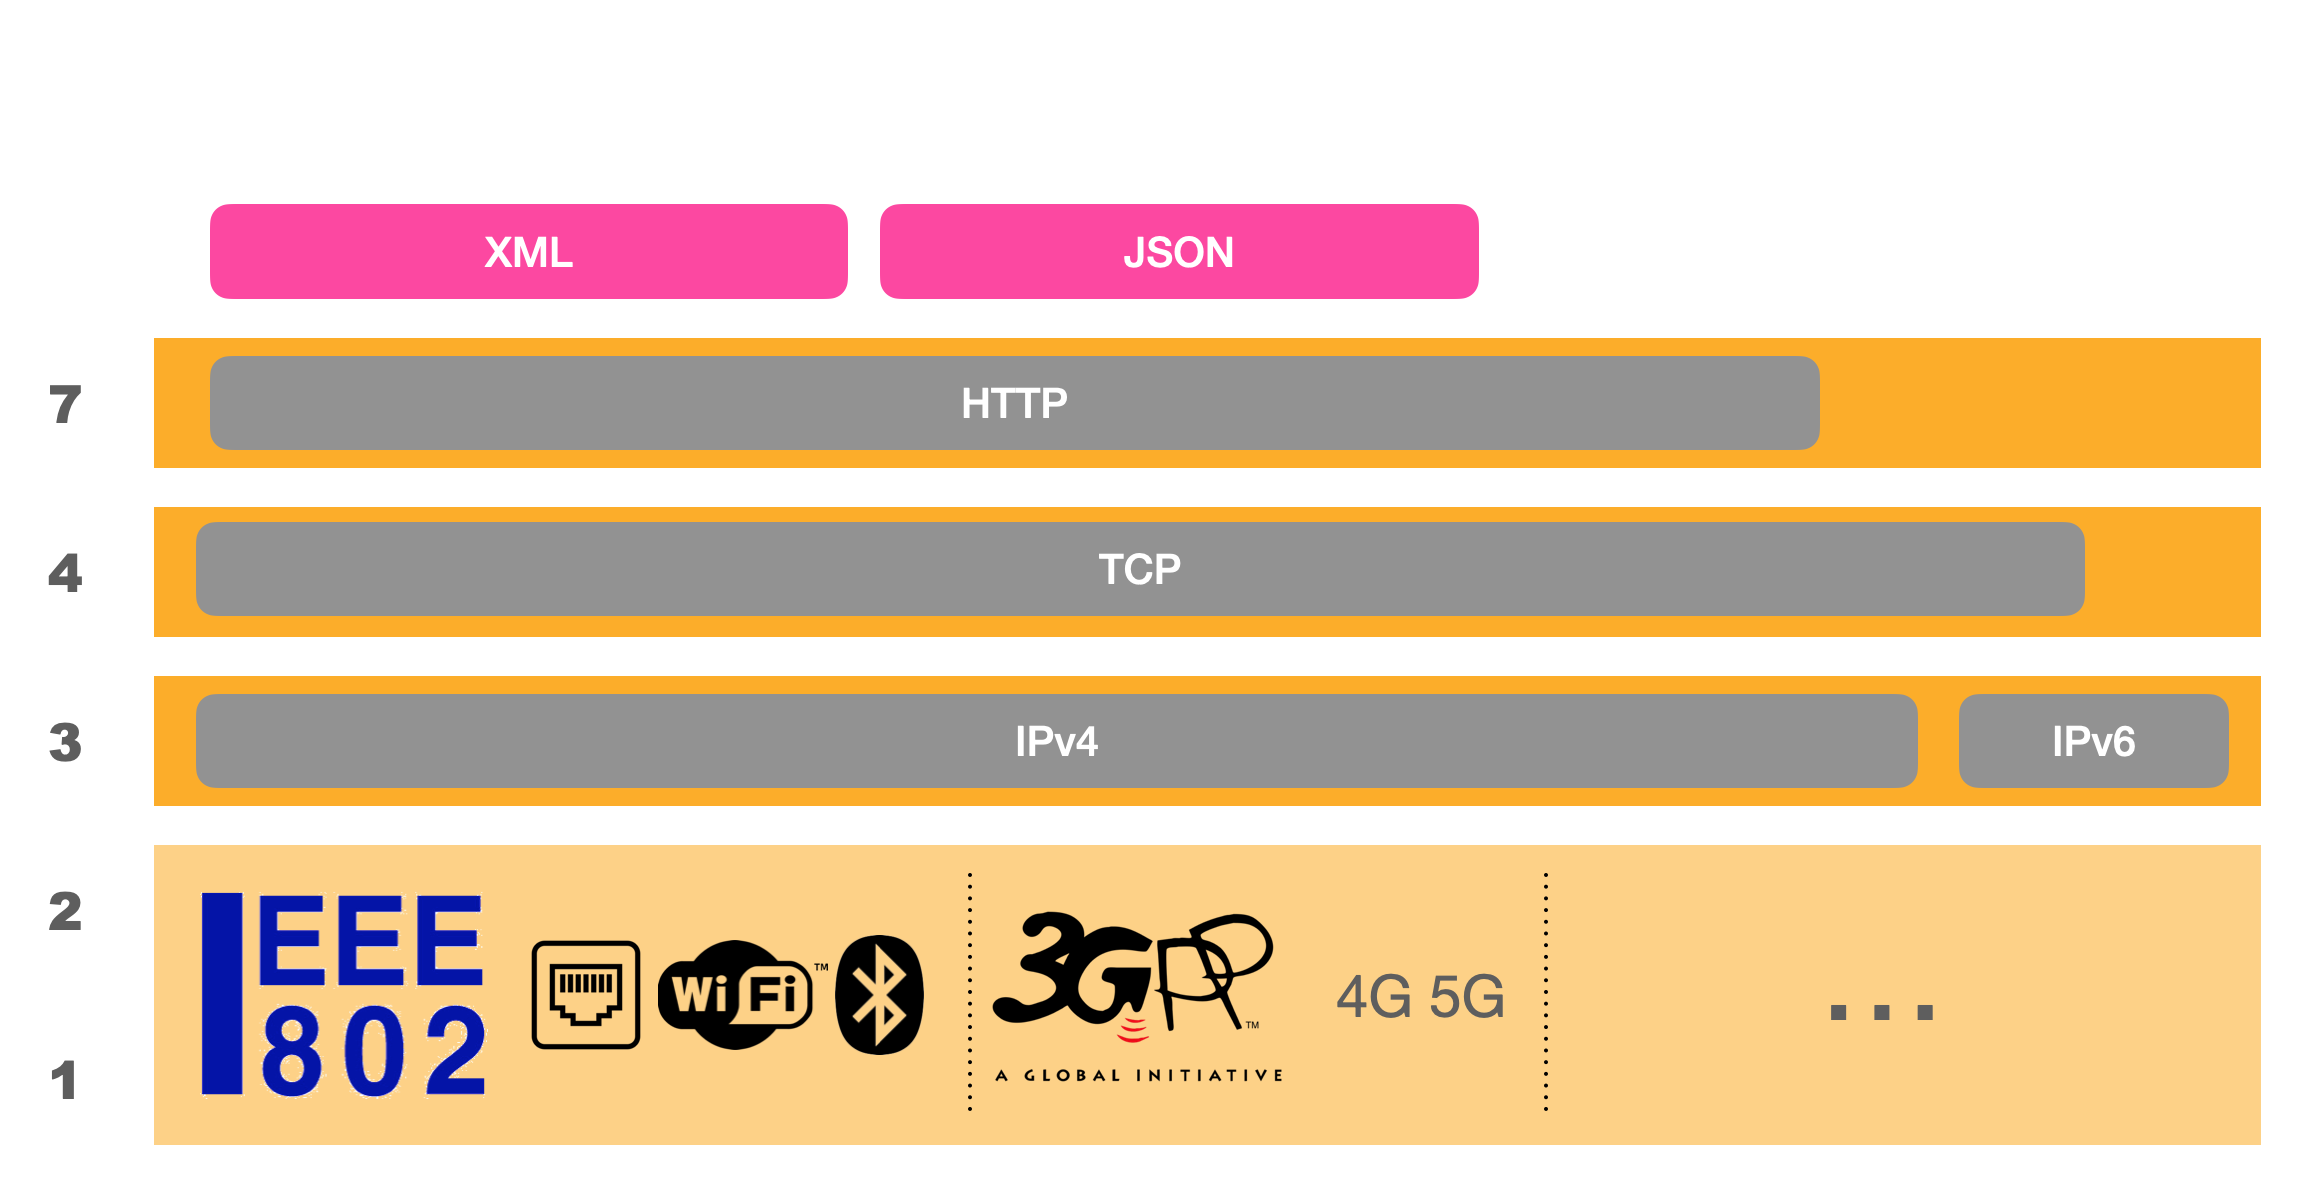
\includegraphics[width=1\columnwidth]{Pictures/fullIPstack.png}}
\caption{Principaux protocoles de l'Internet}
\label{fig-fullstack}
\end{figure}

  Pour le grand public, l’internet désigne surtout la totalité de cet assemblage protocolaire et est souvent confondu avec l’application qui a démocratisé son usage : le Web.  C'est vrai également pour les techniciens, le trafic produit par le Web est largement présent dans l'Internet. Ce schéma, figure~\vref{fig-fullstack} reprend la pile protocolaire majoritairement utilisé dans l'internet. On voit qu'au niveau 3 on a deux versions du protocole \ac{IP} ; la version 4 est la version historiquement déployée et elle a eu tellement de succès qui est de plus en plus difficile d'avoir des adresses \ac{IPv4} pour les machines. Pour permettre au réseau de continuer de fonctionner, une nouvelle version a été développée. \ac{IPv6} rend l'adressage quasi infini avec des adresses sur 128 bits. \ac{IPv6} gagne petit à petit du terrain dans les usages classiques et c'est surtout une brique essentielle pour l'internet des objets. 
  
  Le Web utilise majoritairement le protocole \ac{HTTP}. Et comme \ac{HTTP} repose sur \ac{TCP}, ces deux protocoles sont dominants sur le réseau. 
  
  Finalement ce graphique ajoute une couche supplémentaire, au-dessus de la couche 7, pour indiquer comment les données transportées sont structurées avec des formats comme \ac{XML} ou \ac{JSON} que nous verrons dans la suite.
  
  
  \Question{Pile Protocolaire}
  {Dans la pile protocolaire de l'internet, quels protocoles ont pour fonction d'aiguiller les paquets jusqu'à leur destination (2 réponses) 
  \begin{multicols}{4}
  \begin{itemize}[label=$\square$]
   \item \Wrong{Ethernet}
   \item \Wrong{IEEE}
   \item \Wrong{802.15.5}
   \item \Wrong{Wi-Fi}
   \item \Correct{IPv4}
   \item \Correct{IPv6}
   \item \Wrong{UDP}
   \item \Wrong{TCP}
   \item \Wrong{MQTT} 
   \item \Wrong{HTTP}
   \item \Wrong{CoAP}
   \item \Wrong{XML}
   \item \Wrong{JSON}
  \end{itemize}
  \end{multicols}
  }
  {Le protocole \ac{IP} permet de transporter l'information d'un bout à l'autre du réseau en utilisant les adresses \ac{IP} contenues dans les paquets. Il existe deux versions de ce protocole \ac{IPv4} initialement déployé et \ac{IPv6} qui offre beaucoup plus de capacité d'adressage.}
  
  \section{Les fondements du Web}
  
    \vspace{1em}
\begin{wrapfigure}{r}{3cm}
\Youtube{https://youtu.be/PKKzV-Vy33s}
\end{wrapfigure}

  L'architecture qui a conduit au Web est une formidable source d’inspiration pour le développement de nouveaux services car il est l’un des plus grands succès reposant sur le réseau Internet. Le Web forme de grands systèmes distribués et repose sur plusieurs principes qui le rendent universel et évolutif. La navigation avec un navigateur n’est que la partie visible du trafic ; les principes du web sont également utilisés pour le streaming vidéo, les échanges entre ordinateurs. 
  
  Le Web et ses extensions sont basés sur un modèle client-serveur. Les serveurs possèdent des ressources et les clients peuvent y accéder ou les modifier grâce à un protocole tel que \ac{HTTP}. Le modèle client-serveur est quelque chose de courant dans les réseaux informatiques, mais le Web suit certaines directives de conception connues sous le nom de \ac{REST}.

    \vspace{1em}

Selon Roy Fielding, qui a défini ce modèle~\cite{rest}, \ac{REST} est un ensemble de principes, de propriétés et de contraintes. \ac{REST} utilise le modèle de communication client-serveur et utilise généralement le protocole \ac{HTTP}.

Le principe \ac{REST} permet de concevoir des serveurs évolutifs. Un serveur doit être sans état, ce qui signifie qu’il ne conserve pas d’information après avoir répondu à une demande d’un client. Cela permet de simplifier le traitement dans le serveur qui doit traiter les requêtes d'un grand nombre de clients. 

Cela impose que l’état soit situé du côté du client. Cet état est alimenté à partir des données structurées que le client reçoit du serveur. Ainsi, lorsqu’un client demande une page Web, celle-ci peut contenir d’autres \ac{URI} pour la compléter, par exemple des images, des feuilles de style, des scripts, etc.

Le client doit donc comprendre les données que le serveur lui envoie et donc connaître le format de représentation de la ressource qu'il reçoit pour y retrouver les \ac{URI}. Donc, en plus de la ressource elle-même, le serveur ajoute des informations complémentaires, appelées métadonnées. Elles intègrent entre autres le format du contenu (content format). Il peut s’agir de texte pur, d’une image ou d’un format de texte structuré tel que \ac{HTML} ou \ac{JSON}.
  
      \vspace{1em}

\subsection{Ressources}

    \vspace{1em}

   \begin{wrapfigure}{r}{9cm}
\centerline{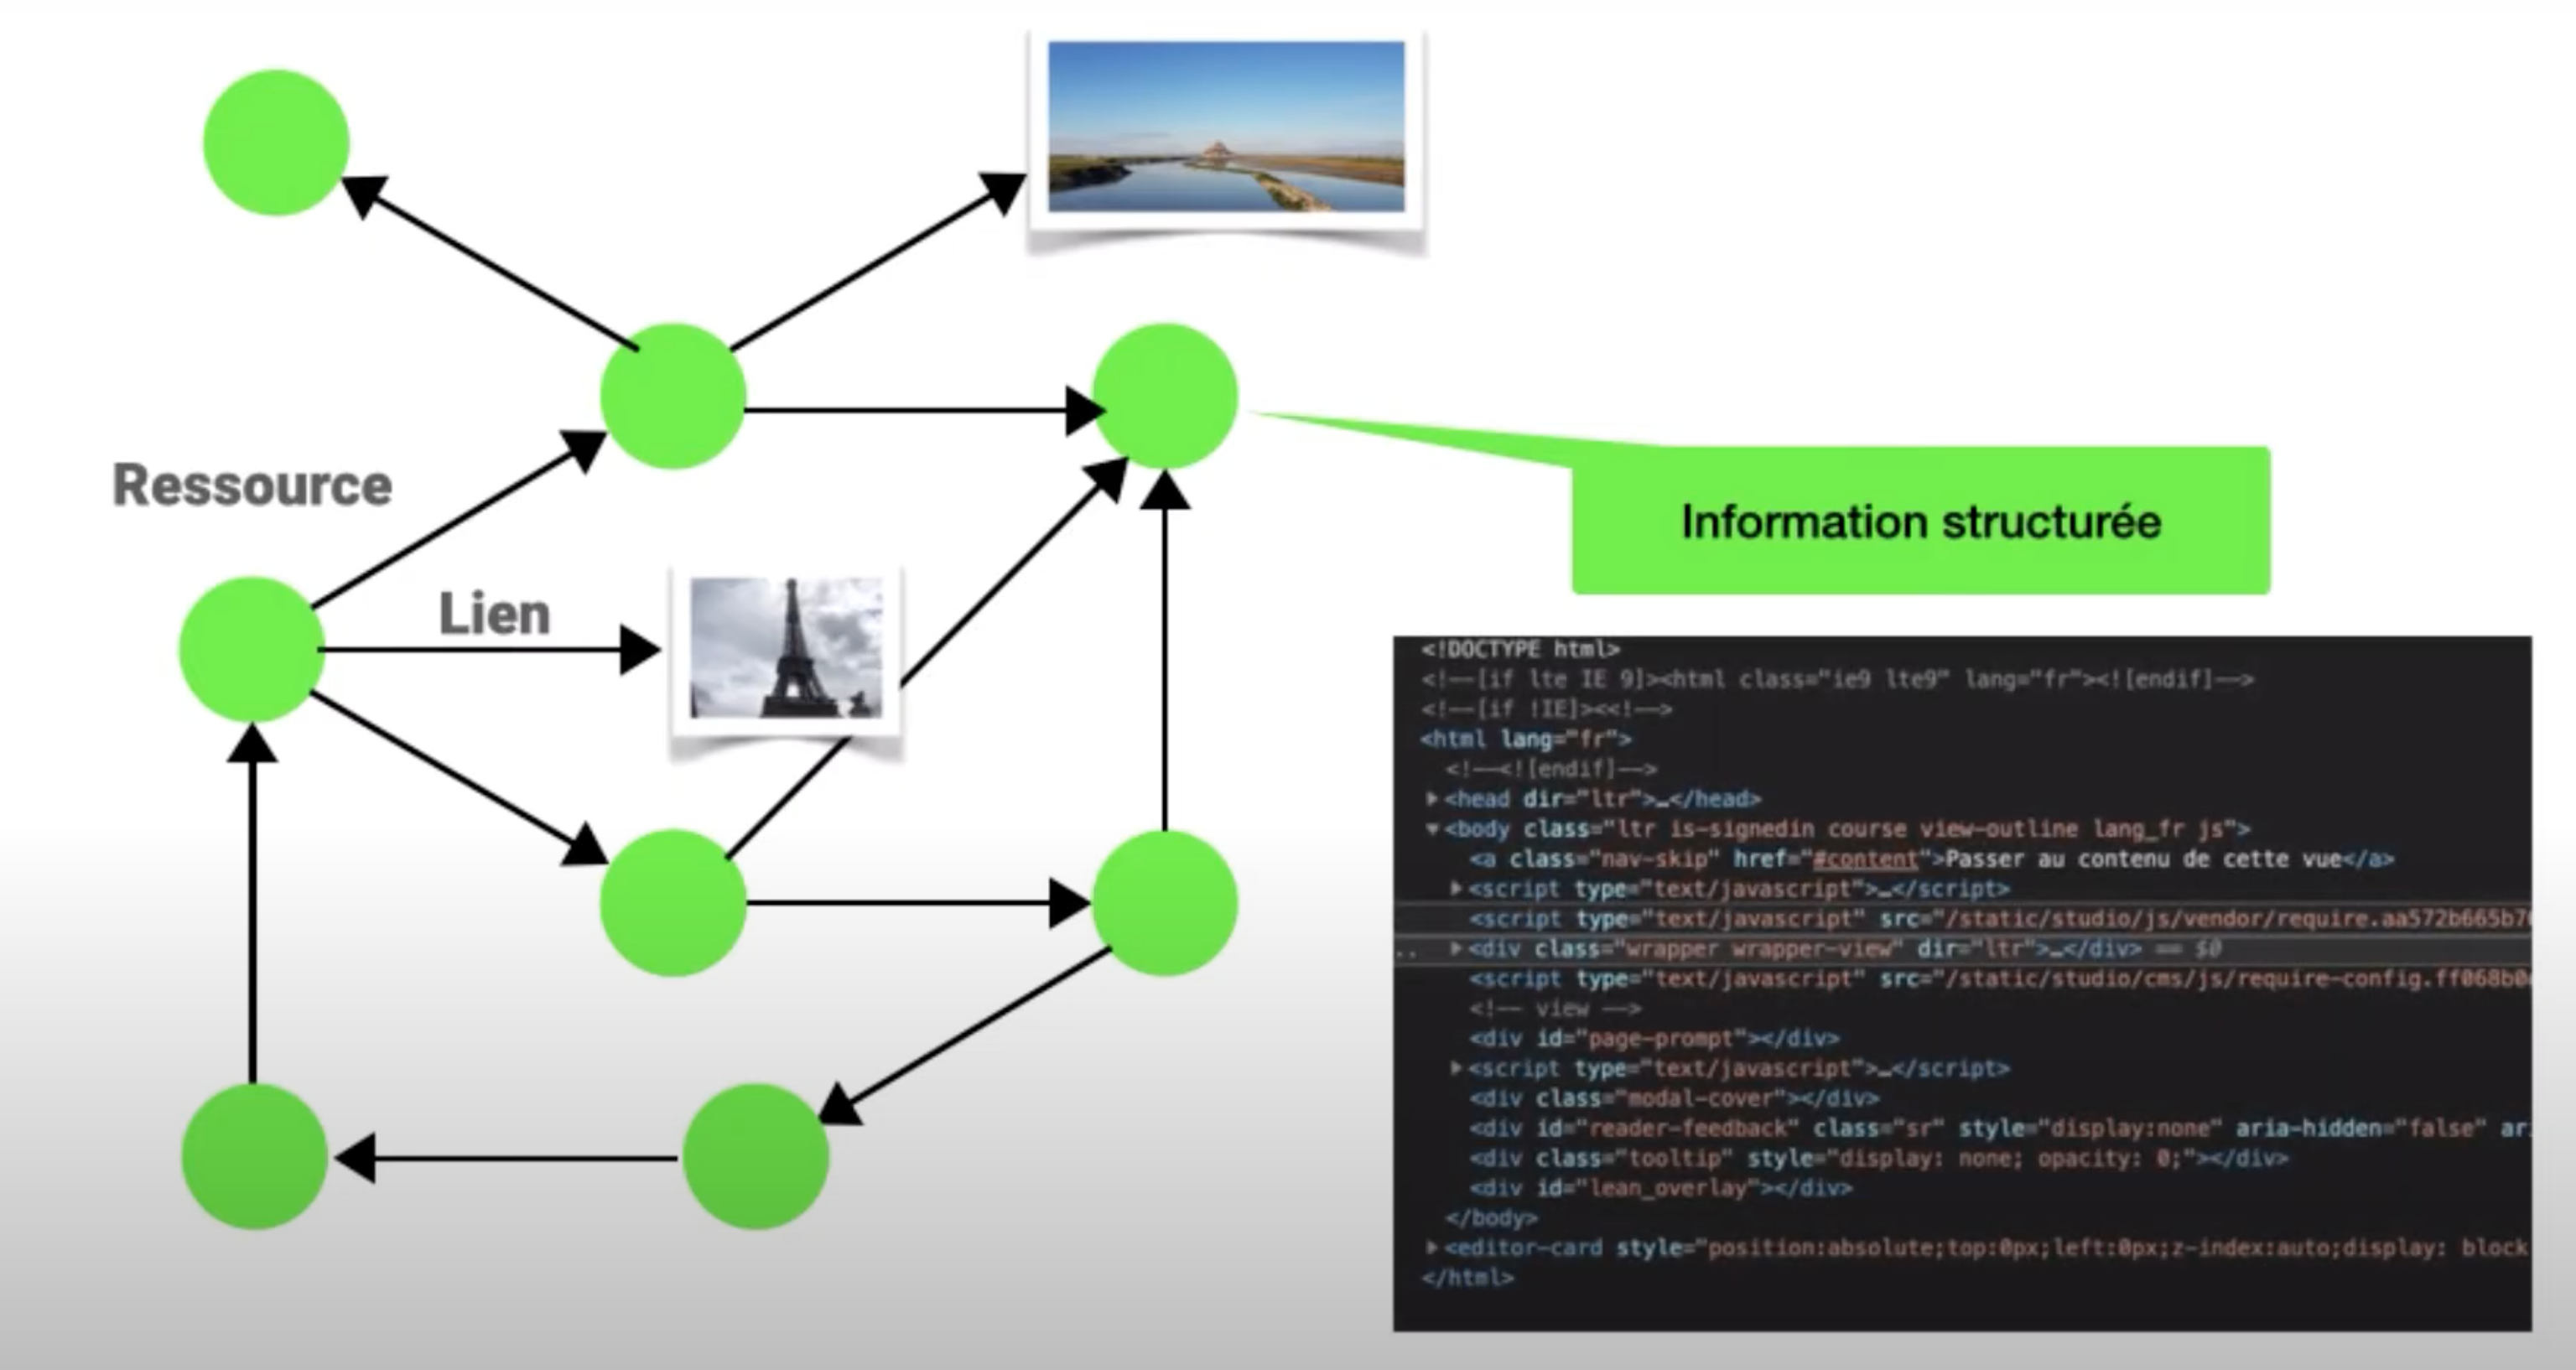
\includegraphics[width=.6\columnwidth]{web.png}}
\end{wrapfigure}
   L'élément de base est la ressource que l'on peut définir comme un bloc de données de taille finie. Les ressources peuvent elles-mêmes contenir des références à d'autres ressources qui à leur tour vont faire référence à d'autres ressources etc. etc. Cela forme un maillage entre ressources qui est comparé à une toile d'araignée (web en anglais). La ressource peut être, par exemple, une image dans ce cas elle ne fera pas référence à autre chose. Pour faire référence à une autre ressource, son contenu doit être structuré et doit donc être défini dans un format où l'on peut facilement comprendre qu'une partie du contenu est une référence a une autre ressource. HTML est un de ces langages qui permet aux pages web de se référencer entre elles par le biais de liens. 
  
      \vspace{1em}

\subsection{identifiants} 

    \vspace{1em}

   
   Chaque ressource du Web est identifiée par une valeur unique appelée \ac{URI}. Si l’URI contient des caractères internationaux, (comme les lettres accentuées, ...)   il est appelé \ac{IRI}.

Les \ac{URI} permettent de désigner une ressource de manière non ambiguë, c'est-à-dire que l'on ne retrouvera pas le même \ac{URI} pour désigner deux ressources différentes.  Par construction, la structure de l’\ac{URI} est hiérarchique, ce qui permet de créer des identificateurs uniques de manière distribuée. Si vous voulez identifier une ressource, vous devez posséder une séquence unique : un numéro de téléphone, un numéro de sécurité sociale, un nom de domaine. En y ajoutant quelque chose d'unique pour nous, cela crée un identifiant globalement unique. 

Par exemple, pour identifier une image, on peut la nommer

\begin{termc}[backgroundcolor=\color{palerod}, language=json, basicstyle=\ttfamily, escapechar=@]
image
\end{termc}

\noindent

mais il y a peu de chance que ce nom soit unique, d'autres personnes sur Terre ont sûrement eu la même idée. En revanche, si je la fais précéder de mon numéro de téléphone

\begin{termc}[backgroundcolor=\color{palerod}, language=json, basicstyle=\ttfamily, escapechar=@]
33667789078image
\end{termc}


\noindent
 sera unique si je ne nomme qu'une seule ressource "image". Un autre utilisateur sur le même principe pourra nommer sa ressource :

\begin{termc}[backgroundcolor=\color{palerod}, language=json, basicstyle=\ttfamily, escapechar=@]
33667239018image
\end{termc}


\noindent
sans ambiguïté possible. Cependant, comme le numéro de téléphone est unique dans l'espace des numéros de téléphone, d'autres numéros uniques pourraient entrer en conflit dans d'autres espaces de numérotation. 

Pour éviter les conflits, il est intéressant de donner, au début l'espace de numérotation, par exemple :

\begin{termc}[backgroundcolor=\color{palerod}, language=json, basicstyle=\ttfamily, escapechar=@]
tel:33667789078image
\end{termc}

\noindent
et

\begin{termc}[backgroundcolor=\color{palerod}, language=json, basicstyle=\ttfamily, escapechar=@]
ss:33667789078image
\end{termc}


\noindent
Les deux identifiants seront uniques, même si le hasard a fait que ce numéro de téléphone et ce numéro de sécurité sociale coïncident.

      \vspace{1em}


Les \ac{URI} formalisent ce principe. Le \rfc{3986} explique comment ils peuvent être construits. Un URI commence par un schéma indiquant l’autorité de nommage, suivi d’une valeur d’autorité puis d’un chemin dans l’espace d’autorité. Des caractères comme les ":" ou les "/" sont utilisés pour améliorer la lisibilité de l'\ac{URI}.



Par exemple~:

\begin{termc}[backgroundcolor=\color{palerod}, language=json, basicstyle=\ttfamily, escapechar=@]
mailto:mduerst@ifi.unizh.ch
ssh://utilisateur@example.com
ftp://ftp.is.co.za/rfc/rfc1808.txt
\end{termc}


      \vspace{1em}

Ainsi, si je mets une ressource sur un site Web, celui-ci est identifié par un nom de domaine, par exemple \texttt{example.com}. Je suis propriétaire de ce nom. Je peux donc l’utiliser pour identifier de manière unique ma ressource. Si on reprend le principe de construction d’un URI, j’aurai :

\begin{termc}[backgroundcolor=\color{palerod}, language=json, basicstyle=\ttfamily, escapechar=@]
http://example.com/ma_ressource
\end{termc}


Personne d’autre dans l’univers ne pourra identifier ses ressources avec cette chaîne de caractères puisque \texttt{example.com} m’appartient. Je dispose donc d’un espace de nommage infini qui me permet de désigner l’ensemble infini de ressources sans que personne d’autre ne puisse prendre les mêmes noms. Un \ac{URI} est une construction administrative permettant d’attribuer un identifiant unique global à une ressource spécifique.


  \begin{figure}[tbp]
\centerline{
\includegraphics[width=1\columnwidth]{Pictures/Capture15.png}}
\caption{Structuration d'une URI}
\label{fig-stucURI}
\end{figure}

L’\ac{URI} (cf.figure~\vref{fig-stucURI}) a pour but de facilement nommer une ressource, de pouvoir lier les ressources entre elles pour former cette toile d’araignée mondiale. Le schéma définit à la fois l'espace de nommage de l'autorité et son format. Une adresse \ac{IP} ou un nom de domaine comme autorité est à la fois un moyen d'assurer l'unicité globale, mais également de savoir comment accéder à la ressource. 

      \vspace{1em}

   Par exemple, \Index{spotify} a défini son propre schéma et ensuite il n'a plus besoin d'autorité mais structure le chemin pour référencer une playlist. 
   
   
   
   Tous les livres ont un numéro \ac{ISBN} qui permet d'identifier. Il peut être intégré aussi dans une URI. Il faut voir que ces deux types d'identifiants permettent de référencer un objet unique mais rien qu'en le lisant on ne peut pas accéder à la ressource. On appelle cette sous famille des \ac{URI}, des \ac{URN}. Si en revanche, en lisant l'URI on peut localiser la ressource on a une \ac{URL}.

Un sous-ensemble d’\ac{URI} peut être directement utilisé pour localiser la ressource, c’est-à-dire trouver sur quel serveur se trouve la ressource et comment y accéder. Il s’agit d’une URL bien connue du grand public et utilisée par les navigateurs Web.

Le schéma http est bien pratique car il peut se lire également comme un \ac{URL}. Ce schéma donne~:

\begin{itemize}
\item le protocole à utiliser pour accéder à la ressource (http),
\item l’autorité qui indique l’adresse du serveur (et son port),
\item et enfin, le chemin d’accès de ce que l'on va demander au serveur et qui peut parfois correspondre à une arborescence de fichiers sur un serveur.
\end{itemize}
   
   
       \vspace{1em}

  Mais il faut bien voir que le but initial est de faire un identifiant unique. Le schéma https donne la manière dont sera construit la suite et dans un second temps uniquement sera vu comme le protocole à utiliser pour accéder à la ressource. L'autorité est unique et dans un second temps servira à localiser le serveur. Et finalement le chemin va indiquer comment parvenir à accéder à la ressource sur le serveur. Donc les ressources de notre toile d'araignée mondiale sont présentes sur des serveurs et chaque ressource possède un identifiant unique. Dans un premier temps, le client connaît l'\ac{URI} d'une ressource. Si c'est une \ac{URL}, il peut contacter le serveur. Le serveur lui retourne la ressource. Le client l'analyse et découvre les \ac{URI} qu'il contient. Il peut donc interroger le ou les autres serveurs pour reconstruire localement une partie de la toile nécessaires au traitement que le client veut effectuer.
  
         \vspace{2em}

\Question{Unicité}{Qu'est ce qui est unique dans le monde (6 réponses) ?
\begin{itemize}[label=$\square$]
\item \Wrong{Un prénom.}
\item \Wrong{Un nom de famille.}
\item \Correct{un numéro de sécurité sociale utilisé en France.}
\item \Correct{un numéro de passeport.}
\item \Correct{un numéro de téléphone portable avec son préfixe international.}
\item \Correct{un numéro complet de compte en banque (\ac{IBAN}).}
\item \Wrong{l'adresse IP de ma machine dans mon réseau privé.}
\item \Correct{l'adresse IP d'un serveur fun-mooc (\texttt{51.255.9.16}).}
\item \Correct{le nom de domaine \texttt{plido.net}.}
\item \Wrong{le nom d'une ville.}
\end{itemize}}
{Ni le prénom, ni le nom de famille, ni leur combinaison ne forment des séquences uniques comme le dirait Jean Dupont.
Les numéros de passeport, de sécurité sociale, de téléphone, de compte bancaire sont par construction uniques dans leur espace, mais il pourrait y avoir des recouvrements. C'est pour cela qu'il faut indiquer la source ou l'autorité qui l'a alloué pour garantir l'unicité. Pour le passeport, l’autorité est le pays qui l’a produit. Le numéro de sécurité sociale correspond au numéro d'inscription au  \ac{RNIPP} (cf. \url{https://www.service-public.fr/particuliers/vosdroits/F33078}). Le code du pays pour le numéro de téléphone est attribué par l'UIT puis chaque opérateur a sa zone de numérotation. Pour le compte bancaire, c’est bien sûr la banque ; chaque banque ayant son propre code contenu au début de l'\ac{IBAN}.
L'adresse IP dans un réseau privé n'est pas unique. Le \rfc{1918} définit des plages d'adresses que tout le monde peut utiliser localement. Pour sortir sur Internet, il faut un dispositif spécial, appelé \ac{NAT}, qui va convertir l'adresse privée en une adresse publique qui, elle, est unique dans le monde. Les serveurs doivent être dans cet espace public et ont donc une adresse unique dans le monde.
Les noms de domaines sont uniques dans le monde par construction mais il peuvent être partagés par plusieurs utilisateurs. On peut donc les étendre comme \texttt{machine1.plido.net}, \texttt{machine2.plido.net}... ou, s'il s'agit de la même machine, ajouter un numéro de port après pour indiquer le service : \texttt{www.plido.net:80}, \texttt{www.plido.net:8080}.
Quant au nom d'une ville, il n'est pas unique. Il faut aussi préciser le pays, voire la région.
}
 

  \subsection{Interactions}
  
         \vspace{1em}

  Les interactions entre clients et serveurs sont très simples. Le client va gérer les interactions avec les ressources sur un serveur. Il peut, par exemple, récupérer une ressource grâce à une méthode \Index{GET}. Il peut également écrire les données dans une ressource existante grâce à une méthode \Index{PUT}. 
  
  Le nombre d'interactions est très limité. \ac{HTTP} ou \ac{HTTPS} est un moyen de mettre en oeuvre ces méthodes. 




\ac{HTTP} est un protocole qui peut être utilisé pour mettre en œuvre un serveur Web les principes de \ac{REST} (qualifié en anglais de \Index{RESTfull}). \ac{HTTP} définit différentes méthodes permettant au client d’interagir avec les ressources sur le serveur~:

\begin{itemize}
    \item \Index{GET} est utilisée pour récupérer la représentation d’une ressource (par exemple page Web, valeur de température d’un capteur, etc.). Par exemple, la figure~\vref{fig-GET} donne le format d’en-tête \ac{HTTP} GET pour récupérer une page Web :

 \begin{figure}[tbp]
\centerline{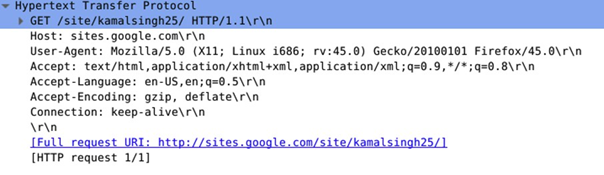
\includegraphics[width=1\columnwidth]{Pictures/GET.png}}
\caption{Contenu d'une requête HTTP GET}
\label{fig-GET}
\end{figure}

\item  \Index{HEAD} est utilisée pour récupérer uniquement les métadonnées présentes dans les en-têtes de réponse sans le corps de réponse ;
\item  \Index{POST} est utilisée pour indiquer au serveur une nouvelle ressource  ;
\item  \Index{PUT} est utilisée pour stocker une ressource à l’endroit identifié par l’\ac{URI} dans la requête. Si la ressource existe déjà, elle sera modifiée ;
\item \Index{PATCH} permet au client de ne modifier qu’une partie de la ressource ;
\item  \Index{DELETE} est utilisée pour supprimer la ressource définie.


\end{itemize}

 \Question{Etat}{Est-ce que le serveur garde un état des précédentes requêtes ?
\begin{itemize}[label=$\circ$]
\item \Wrong{Oui}
\item \Correct{Non}
\end{itemize}}
{Le serveur répond à une requête puis passe à la suivante. Il ne garde pas d'état. En revanche, une requête peut servir à modifier le contenu d'une ressource.}

\Question{Wold Wide Web}{Le World Wide Web est basé sur ce principe des états pour :
\begin{itemize}[label=$\circ$]
\item \Wrong{fonctionner à la fois sur des ordinateurs et des téléphones portables,}
\item \Correct{pouvoir servir un grand nombre de requêtes}

\item \Wrong{chiffrer les communications,}
\end{itemize}}
{Voir le commentaire précédent}

 \Question{Repésentation de l'Information}
  {Quels sont les formats qui permettent de représenter des informations structurées (2 réponses)~: 
  \begin{multicols}{4}
  \begin{itemize}[label=$\square$]
   \item \Wrong{Ethernet}
   \item \Wrong{IEEE}
   \item \Wrong{802.15.5}
   \item \Wrong{Wi-Fi}
   \item \Wrong{IPv4}
   \item \Wrong{IPv6}
   \item \Wrong{UDP}
   \item \Wrong{TCP}
   \item \Wrong{MQTT} 
   \item \Wrong{HTTP}
   \item \Wrong{CoAP}
   \item \Correct{XML}
   \item \Correct{JSON}
  \end{itemize}
  \end{multicols}
  }
  {Il s'agit de XML et JSON qui permettent d'envoyer des données stucturées. Les autres propositions indiquent des protocoles de transport de l'information de niveau 2, 3, 4 et 7.}
  
\Question{Schéma}{Dans l'URI \texttt{https://plido.net/unit/definition.html}, quel est le schéma ?\newline}
{\noindent\texttt{http}~: le Schéma indique comment sera construite l'URI}

\Question{Authorité}{Dans l'URI \texttt{https://plido.net/unit/definition.html}, quel est l'autorité ?\newline}
{\noindent\texttt{plido.net}~: il s'agit de la séquence globalement unique.}


\section {Modèle Publish/Subscribe}

Il existe d’autres formalismes que REST. Un autre formalisme, très populaire, est orienté "diffusion" en utilisant le principe ”publier/abonner” ou ”publish/subscribe”. Comme nous allons le montrer dans la suite, même si les fonctionnalités entre ces deux modes peuvent sembler similaires, la philosophie de conception est très différente : publish/subscribe vise des applications intégrées tandis que REST vise l’interopérabilité globale. 

Le modèle publish/subscribe fait le découplage entre l’expéditeur d’un message et son destinataire. Dans ce paradigme (cf. figure ci-dessous), il existe des ”Publishers” qui produisent des données ou des messages et envoient le message à une entité généralement appelée ”Broker”. En outre, les messages peuvent être classés en ”Topics”, contenus ou types, etc. Ensuite, il existe des abonnés qui souscrivent au broker, par exemple à un topic donné, afin de recevoir les messages qui les intéressent, comme montré dans le schéma.

Le broker peut alors utiliser des filtres pour envoyer uniquement ces messages aux abonnés du topic concerné. Il existe plusieurs protocoles Publish-Subscribe tels que MQTT (Message Queuing Telemetry Transport), AMQP (Advanced Message Queuing Protocol), JMS (Java Messaging Service) ou XMPP (Extensible Messaging Protocol et Présence).

\subsection{MQTT}

MQTT est détaillé dans la suite du cours car il est très populaire pour la communication entre processus, mais également dans l’internet des objets.

Imaginons par exemple que plusieurs capteurs soient installés dans deux bâtiments A et B. Certains capteurs collectent des informations sur la température et d’autres collectent des informations sur l’humidité. Ces capteurs peuvent envoyer les données régulièrement à un broker central.

Les données peuvent être classées en différentes rubriques qui peuvent également être organisées de manière hiérarchique. Par exemple, le topic /sensor signifie "toutes les données de capteurs", \texttt{/sensor/buildingA/} signifie "des données de capteurs uniquement installées dans le bâtiment A". En plus, \texttt{/sensor/buildingA/temperature} pourrait signifier "des données de capteurs de température installés uniquement dans le bâtiment A".

Certains abonnés peuvent s’abonner aux messages en fonction de leur intérêt. Ainsi, un abonné intéressé uniquement par les données d’humidité du bâtiment B peut s’abonner au sujet \texttt{/sensor/buildingB/humidity} et le broker n’enverra que ces données à cet abonné.

\subsection{différence avec REST}

Les principaux avantages du paradigme publish-subscribe par rapport au paradigme client-serveur, tels qu'inclus en REST, sont les suivants :
\begin{itemize}
\item faible couplage entre émetteur et récepteur, le broker sert d'intermédiaire et stocke les informations ;
\item passage à l’échelle. Les données provenant d'une source ne sont émises qu'une fois par la source. Le broker les recopie vers tous les abonnés. Dans un mode client/serveur, les données doivent être émises par le serveur autant que fois que les clients le demandent.
\end{itemize}
L’absence de couplage entre l’expéditeur et le destinataire se fait en termes d’espace, de temps et de synchronisation. Celui qui publie les données a une tâche simplifiée. Il n'a pas à gérer ou connaître ceux qui les consomment, il n'a qu’à les envoyer au broker.

MQTT est très léger et conçu pour les périphériques de faibles puissances. Il a une très petite empreinte logicielle et est optimisé pour fonctionner dans les environnements à faible bande passante. Cela rend MQTT idéal pour les applications IoT. Malgré tout, l’usage de TCP et des très nombreux acquittements peut s’avérer lourds pour les équipements ou les réseaux très contraints. Une version plus légère basée sur UDP existe pour ces cas d’usage, mais elle est peu utilisée.

S'ils se ressemblent, les principes de nommage des topics MQTT et des URI REST sont complètement différents. Par rapport à MQTT, le chemin dans l'URI n'a pas de sémantique. Il a juste vocation à être unique. Il ne peut pas être utilisé pour agréger plusieurs sources d'information. Si deux capteurs publient respectivement sur les topics \texttt{/sensor/buildingA/temperature} et \texttt{/sensor/buildingB/temperature}, un subscriber peut s'abonner au topic \texttt{/sensor/*/temperature} pour recevoir toutes les mesures ; ce qui est impossible avec REST : il faudra autant de requêtes que de capteurs pour récupérer l'ensemble des mesures.

Les URI sont simplement uniques au monde par leur construction alors que les topics du MQTT sont spécifiques à une application. Un topic MQTT peut être interprété différemment par deux applications différentes. Cela ne permet pas une interopérabilité sémantique. Les abonnés doivent être construits avec une connaissance des topics utilisés par les publieurs.

%\chapter {Wireshark}

\Index{Wireshark} va être notre ami dans la suite de cet ouvrage pour comprendre le fonctionnement des protocoles et analyser les données qui vont circuler. Malheureusement, dans certains cas, nous devons avoir recours à des outil plus rustiques comme des traces en \Index{hexadécimal}\footnote{\url{https://fr.wikipedia.org/wiki/Syst\%C3\%A8me\_hexad\%C3\%A9cimal}} (base 16).  Il faut donc se familiariser avec ces outils, ce que nous allons faire dare-dare en analysant des requêtes HTTP simples.

\section{Installation}

L'installation de Wireshark se fait en allant sur le site éponyme \url{https://www.wireshark.org/}, soit sous Linux en installant le paquetage \texttt{wireshark}. Ce programme nécessite des droits particuliers pour accéder aux messages venant du réseau, il faut les accorder au moment de l'installation.

\section{Démarrage}

Si vous lancez Wireshark avec les bon privilèges, la fenêtre d'accueil va afficher les interfaces disponibles, comme le montre la figure~\vref{fig-wires-open} sur Windows. En regard avec le modèle de référence de l'\ac{ISO}, il s'agit des protocoles de niveau 2 présent sur l'ordinateur. Il peut s'agit d'une carte physique comme Ethernet ou Wi-Fi ou d'interface virtuelle utilisées pour communiquer en interne sur l'ordinateur. 

\begin{figure}[tbp]
\centerline{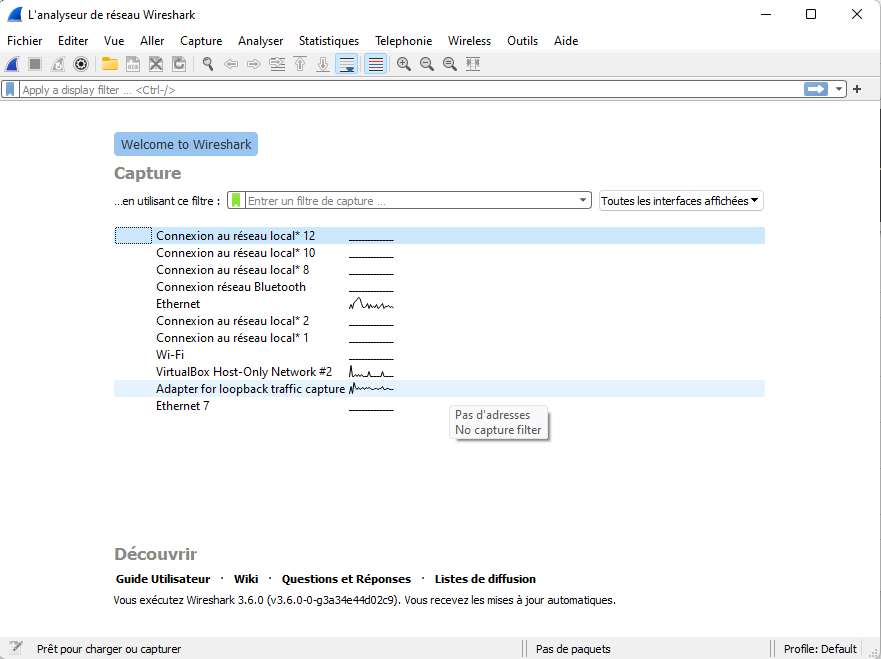
\includegraphics[width=1\columnwidth]{Pictures/wireshark-open.png}}
\caption{Ouverture de Wireshark}
\label{fig-wires-open}
\end{figure}


Il s'agit de déterminer quelle interface choisir. Ce n'est pas toujours facile car leurs noms ne sont pas toujours très explicites. Les petites courbes à gauche du nom indiquent le trafic instantané que Wireshark mesure. Sur le schéma, 3 interfaces sont actives : Ethernet, la communication avec une machine virtuelle et une interface appelée \textit{\Index{loopback}}.  La première permet d'avoir les communications avec l'extérieur et la dernière sera très utile lors des échanges entre deux processus dans cette machine.

\section {Capture}

En cliquant sur le nom de l'interface donnant accès au réseau exterieur (\index{Ethernet} dans notre cas), la fenêtre se découpe en 3 parties, comme le montre la figure~\vref{fig-wires-cap}.

\begin{figure}[tbp]
\centerline{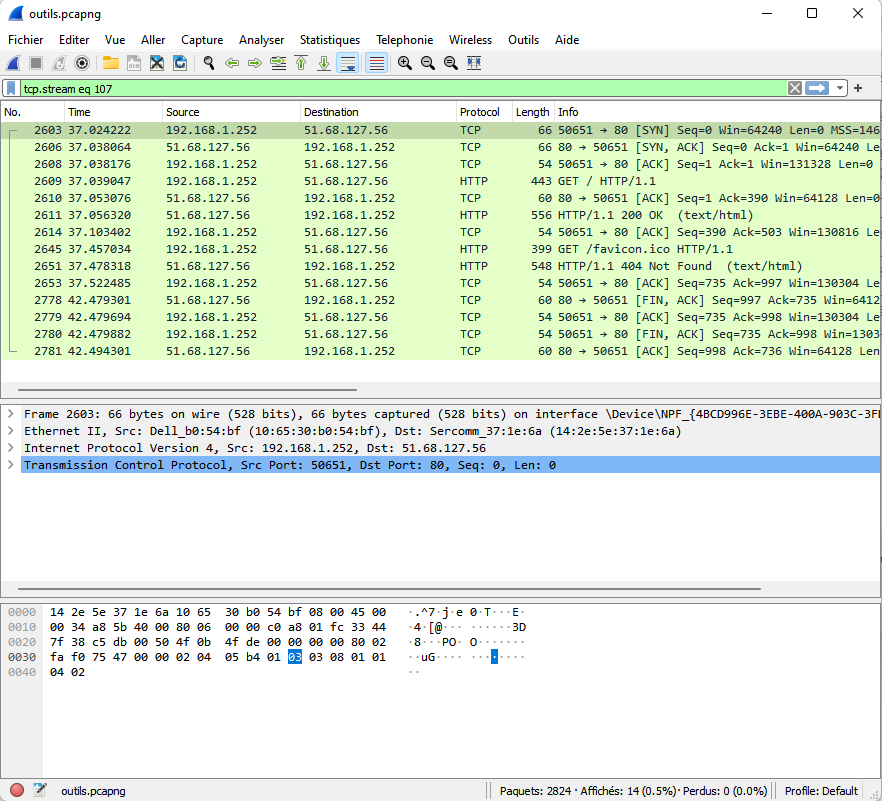
\includegraphics[width=1\columnwidth]{Pictures/ws-capture.png}}
\caption{Capture du trafic}
\label{fig-wires-cap}
\end{figure}

L'écran de Wireshark se divise en 3 parties :
\begin{itemize}
\item en haut, défile les trames qui sont capturées sur le réseau, chaque protocole à une couleur dédiée pour facilité le repérage~:
\begin{itemize}
\item le numéro de trame capturée, il s'agit d'une information ajoutée par Wireshark,
\item l'heure de capture de la trame. Cette information est aussi ajoutée par Wireshark,
\item l'adresse IP (IPv4 ou IPv6) de la machine à l'origine du paquet, 
\item l'adresse IP (IPv4 ou IPv6) de la machine destinataire du paquet,
\item le protocole de plus haut niveau contenu dans la trame. Dans notre cas, cela peut être TCP si le message TCP ne contient pas de données, comme lors de l'ouverture de connexion, ou de certains acquittements. On voit également les messages \ac{HTTP} qui sont bien entendu encapsulés dans TCP,
\item la taille en octets de la trame capturée par Wireshark,
\item finalement Wireshark fourni un résumé du contenu de la trame, pour comprendre ce qui se passe sur le réseau. Dans la capture, on retrouve pour les messages \ac{HTTP}, les requêtes GET ou les notifications ;
\end{itemize}
\item si une trame est sélectionnée dans la liste, elle apparaît dans la zone du milieu avec l'empilement protocolaire. Le contenu de chacun de ces protocoles peut être détaillé en cliquant sur le petit triangle à gauche ;
\item la fenêtre du bas donne l'équivalent en hexadécimal. Les parties surlignées correspondent aux champs sélectionnés dans la fenêtre du milieu. À noter que l'on retrouve l'information à la fois en hexadécimal et en caractère \ac{ASCII}, ce qui aide à la lecture quand on cherche une valeur spécifique.
\end{itemize}

\Question{Première colonne}
{Dans la première colonne~:
 \begin{itemize}[label=$\circ$]
   \item \Correct{Le numéro de la trame attribué par Wireshark à sa réception}
   \item \Wrong{Le numéro de la trame relevé directement dans la trame Ethernet}
  \end{itemize}
}
{
Ces numéros sont séquentiels, ils sont donc attribué localement par Wireshark. De plus il n'existe aucun champ de cette sorte dans Ethernet.
}
\Question{Deuxième colonne}
{Dans la deuxième colonne~:
 \begin{itemize}[label=$\circ$]
   \item \Correct{L'heure de réception par Wireshark}
   \item \Wrong{L'instant d'émission de la trame}
  \end{itemize}
}
{
Comme dans le cas précédent, ce numéro est ajouté par Wireshark, il n'existe pas de champ protocolaire indiquant l'instant d'émission.
}
\Question{Les troisième et quatrième colonnes}
{Dans les troisième et quatrième colonnes~:
 \begin{itemize}[label=$\circ$]
   \item \Wrong{les adresses Ethernet des machines.}
   \item \Wrong{Uniquement les adresses IPv4 des machines.}
   \item \Correct{Les adresses IPv4 ou IPv6 des machines.}
  \end{itemize}
}
{
Wireshark traite de la même manière les adresses IPv4 ou IPv6, elles sont donc affichées dans ces colonnes. L'adresse Ethernet (ou MAC) sur 48 bits n'est pas affichée par défaut dans cet écran.
}

\Question{La cinquième colonne}
{Dans la cinquième colonne~:
 \begin{itemize}[label=$\circ$]
   \item \Wrong{Le protocole applicatif (niveau 7).}
   \item \Correct{Le dernier (de plus haut niveau) protocole reconnu.}
   \item \Wrong{Le protocole de niveau 4 (ici TCP ou UDP).}
  \end{itemize}
}
{
Wireshark fournit l'information de plus haut niveau. Dans la figure~\vref{fig-wires-cap} certaines trames sont indiquées comme transportant le protocole HTTP, tandis que d'autres, généralement les acquittements sont indiqués comme étant de type TCP car elles ne transportent pas de données venant des couches supérieures.
}
\Question{La sixième colonne}
{Dans la sixième colonne~:
 \begin{itemize}[label=$\circ$]
   \item \Wrong{La taille en bits de la trame.}
   \item \Correct{La taille en octets de la trame.}
  \end{itemize}
}
{
L'unité est l'octet.
}
\Question{La septième colonne}
{Dans la septième colonne~:
 \begin{itemize}[label=$\circ$]
   \item \Correct{Un résumé des informations transportées par le protocole de plus haut niveau.}
   \item \Wrong{Les options d'IPv4.}
   \item \Wrong{le contenu en ASCII du message de plus haut niveau.}
  \end{itemize}
}
{
Wireshark cherche a interpréter les champs du protocole de plus haut niveau pour offrir un affichage synthétique de l'information.}
  \vspace{1em}

Cela fait beaucoup de trafic, nous allons limiter ce qui est affiché en ajoutant un filtre à un destinataire particulier. Le site \texttt{outils.plido.net} à l'adresse IPv4 \texttt{51.68.127.56}. Dans la fenêtre où il est indiqué \textit{Apply a display filter.} taper les instructions suivante: 

\begin{verbatim}
    ip.addr==51.68.127.56
\end{verbatim}

\noindent n'oubliez par le double \texttt{==} et la fenêtre doit devenir verte quand tout sera tapé indiquant que la syntaxe du filtre est correcte. En appuyant sur entrée, la fenêtre doit se vider.

\section{Analyse du trafic web}

Dans la barre d'adresse de votre navigateur préféré, taper l'URL suivante:

\begin{verbatim}
    http://outils.plido.net
\end{verbatim}

\noindent et la page Web indiqué figure~\vref{fig-firefox-hello} doit apparaître. 

\begin{figure}[tbp]
\centerline{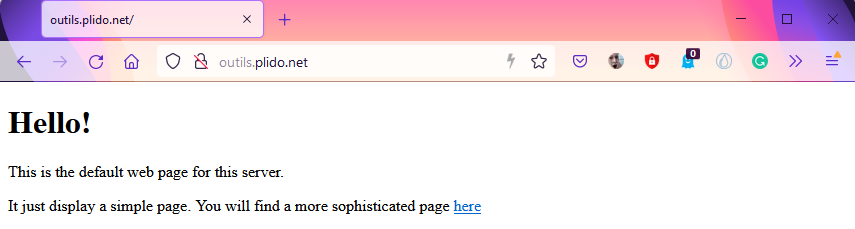
\includegraphics[width=1\columnwidth]{Pictures/firefox-simple.png}}
\caption{Afficher de la page par Firefox}
\label{fig-firefox-hello}
\end{figure}

  \vspace{1em}

Wireshark a permis de visualiser le trafic échangé entre l'ordinateur et le serveur Web. Le trafic doit être similaire a celui de la figure~\vref{fig-wires-cap}. La figure s'obtient en sélectionnant le menu \textit{Statistiques/Graphique de flux} et en cochant \textit{Limiter au Filtre d'Affichage}. Elle est un peu plus lisible car elle représente les échanges sous forme de chronographes.

\begin{figure}[tbp]
\centerline{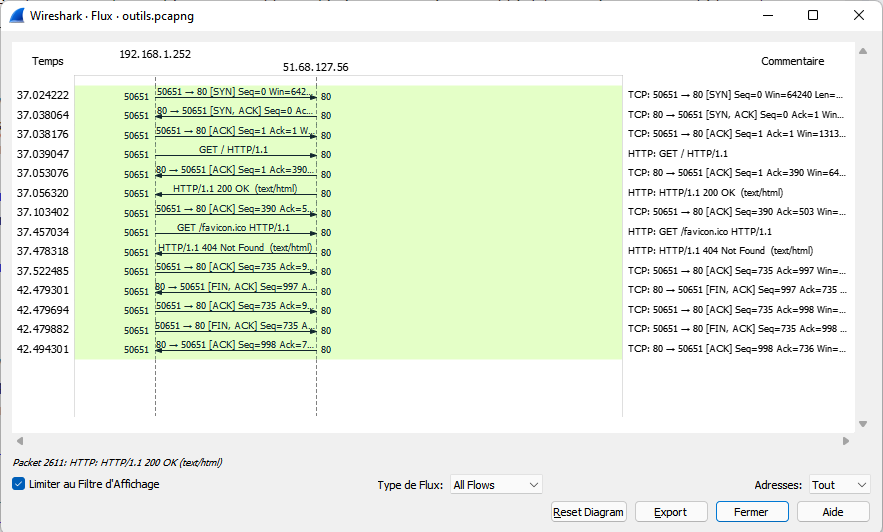
\includegraphics[width=1\columnwidth]{Pictures/ws-filtre.png}}
\caption{Afficher de la page par Firefox}
\label{fig-ws-filtre}
\end{figure}

Trois phases peuvent être distinguées~:
\begin{itemize}
    \item L'ouverture de connexion TCP avec l'émission de trois messages TCP;
    \item la phase de transfert de données~:
    \begin{itemize}
        \item le client envoie une requête HTTP GET au serveur pour demander la ressource à la racine (\texttt{/}),
        \item le serveur acquitte le message au niveau TCP pour indiquer qu'il a bien été reçu.
        \item le serveur envoie la réponse à la requête précédente et précisant le statut (\textttt{200 : OK}) et le que contenu est formaté en HTML.
        \item le client acquitte ce message au niveau TCP
        \item le client envoie une nouvelle requête HTTP GET pour obtenir la ressource \texttt{/facicon.ico}
        \item le serveur répond que la ressource n'existe pas (\texttt{404 : Not Found}). Cette requête acquitte implicitement le message précédent.
        \item le client acquitte la réponse du serveur au niveau TCP.
    \end{itemize}
    \item le serveur termine la connexion après 5 secondes d'inactivité. La fermeture se fait en échangeant 4 messages TCP.
\end{itemize}

%

%%%%%%%%%%%%%%%%%%%%%%%%%%%%%%%%%%%%%%%%%%%%%%%

% ModBus

%%%%%%%%%%%%%%%%%%%%%%%%%%%%%%%%%%%%%%%%%%%%%%%

\chapterimage{pano-tv1.png} % Chapter heading image

\chapter{Modbus}

\section{Introduction}
  \begin{wrapfigure}{r}{3cm}
\Youtube{https://youtu.be/Jj9Tmci7gXU}
\end{wrapfigure}
 \Index{Modbus} est apparu en 1979 à une époque où l'internet n'existait pas encore ! Il est toujours très populaire dans l'industrie. A l'origine Modbus était construit sur un bus série \Index{RS-485} qui connectait différents équipements  appelé (cf. figure~\vref{fig-modbus1})~:
 \begin{itemize}
 \item secondaires ou slaves et 
 \item un primaire appelée aussi master qui gère les communications. 
 \end{itemize}
 
 
 
 \begin{figure}[tbp]
\centerline{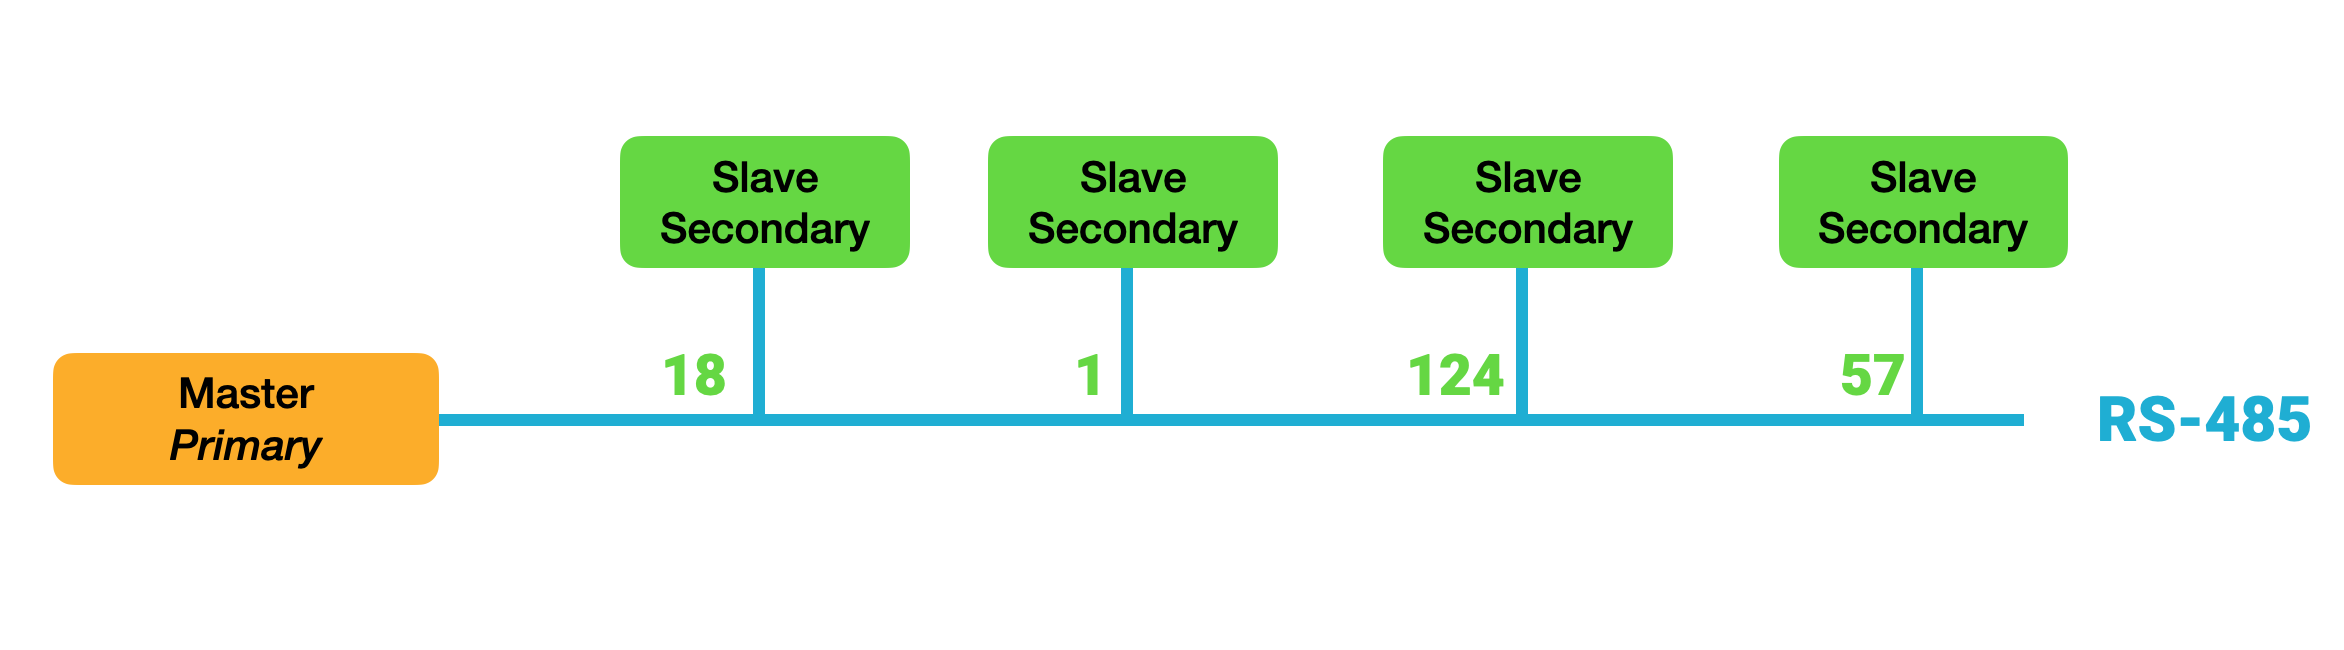
\includegraphics[width=1\columnwidth]{Pictures/Capture35.png}}
\caption{Architecture filaire de Modbus}
\label{fig-modbus1}
\end{figure}

 
 
 Chaque secondaire à un numéro unique ou adresse. Les adresses sont comprises entre 1 et 247. Le primaire n'a pas besoin d'une adresse puisque toutes les communications ont lieu avec lui. 
 
   \vspace{1em}


 Le primaire envoie une requête à un secondaire et le secondaire répond au primaire. Les communications directes entre deux secondaires ne sont pas possibles. 
 
 \subsection{Registres}
 
 
 Un équipement de Modbus peut prendre deux choses à travers des registres : 
 \begin{itemize}
     \item les relais qui peuvent prendre une valeur binaire "on" ou "off". Si le primaire peut modifier l'état et, bien sûr le lire, c'est appeler un \textit{\Index{coil}}. Si la valeur binaire peut uniquement être lu c'est un \textit{\Index{discrete input}}.
     \item des registres sur 16 bits. Ils sont utilisés pour représenter une valeur comme un courant électrique, une température, une vitesse de rotation,... De même, si on peut uniquement lire la valeur à est appelée un \textit{\Index{input register}} sinon, si elle peut être également être modifiée par le primaire, elle est appelée un \textit{\Index{holding register}}.
 \end{itemize}
 
    \vspace{1em}

 
Un équipement Modbus peut avoir jusqu'à 10~000 registres de ces quatre catégories. 

\subsection{Protocole}

Modbus est un protocole requête/réponse. Le primaire envoie une requête à l'adresse d'un équipement pour lire ou écrire un de ces registres. 
\begin{figure}[tbp]
\centerline{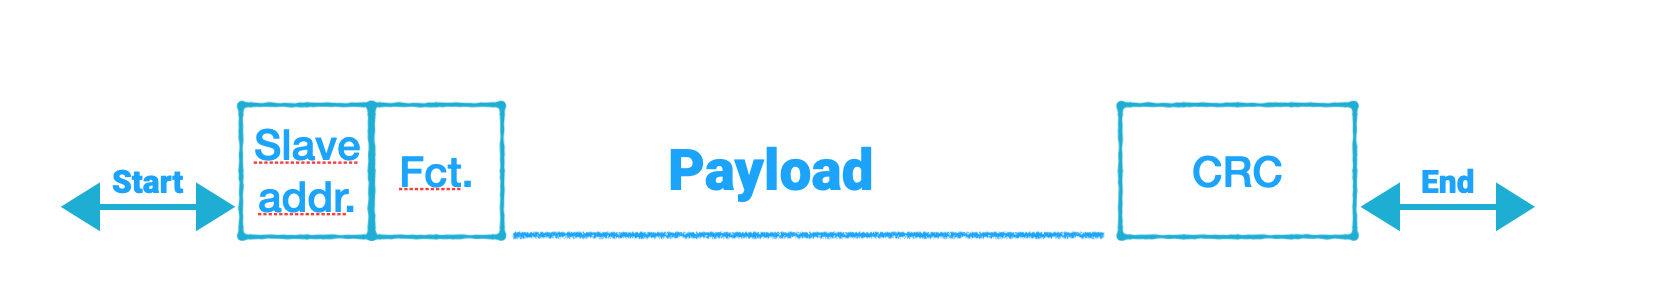
\includegraphics[width=1\columnwidth]{Pictures/Capture37.png}}
\caption{Trame Modbus}
\label{fig-modbus2}
\end{figure}

 

Une trame Modbus est une séquence de caractères commençant par un octet avec l'adresse du secondaire suivi d'une commande ou code de fonctions spécifique à chaque catégorie de registre~:
\begin{itemize}
    \item 1 pour lire un coil,
    \item 2 pour lire un discrete input,
    \item 3 pour lire un holding register,
    \item 4 pour lire un input register,
    \item 5 pour écrire un coil,
    \item 6 pour écrire un holding register,
\end{itemize}

    \vspace{1em}

La suite de la trame contient les données puis un \ac{CRC} pour valider qu'il n'y a pas d'erreur de transmission dans la trame. La partie donnée peut être différente dans la requête et la réponse. Par exemple pour lire un holding register, la requête contient l'adresse du premier registre à lire et le nombre de registres à lire et la réponse contient le nombre de données transmises suivi de leurs valeurs. Pour écrire sur un registre, les données de la trame seront l'adresse du registre et les données à écrire.

\subsection{Exemple: XY-MD02}


Regardons de plus près un exemple concret. On va utiliser un capteur de température et d'humidité, le \Index{XY-MD02} (cf. figure~\vref{fig-XYMD02}) dont les spécifications sont facilement accessibles via une recherche sur Internet. 

\begin{figure}[tbp]
\centerline{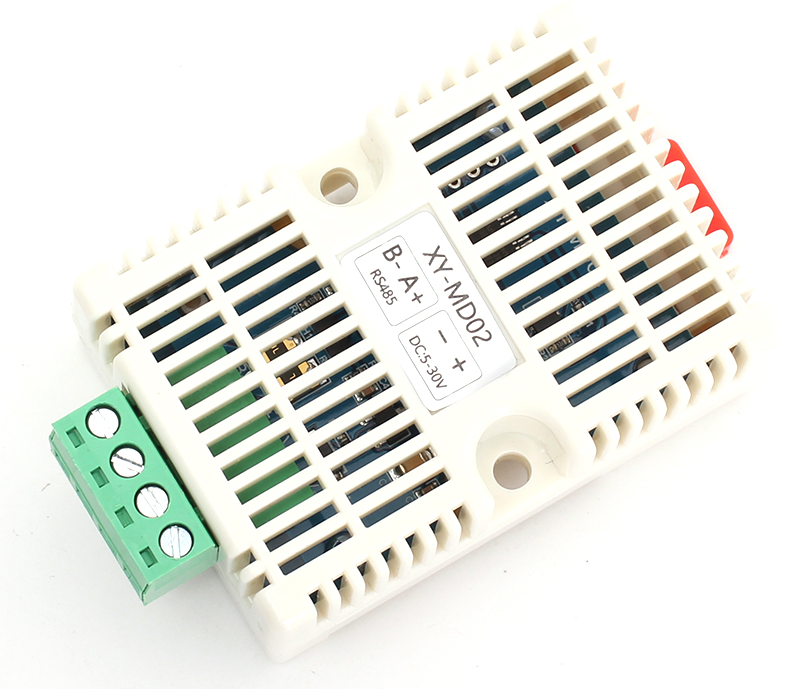
\includegraphics[width=0.6\columnwidth]{Pictures/XY-MD02.png}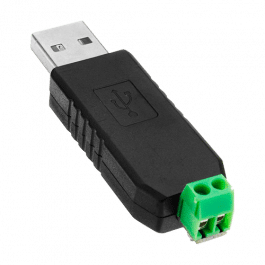
\includegraphics[width=0.4\columnwidth]{Pictures/rs485-usb.png}}
\caption{XY-MD02 et Adaptateur USB/RS-485}
\label{fig-XYMD02}
\end{figure}

La partie verte, se compose de quatre connecteurs dont la signification est indiquée sur l'étiquette. Les deux bornes de gauche constituent le bus \Index{RS-485} nommées \texttt{A+} et \texttt{B-} et les deux bornes de droites permettent d'alimenter électriquement l'équipement avec une tension comprise entre 5V et 30V.

    \vspace{1em}

 \begin{wrapfigure}{r}{3cm}
\Youtube{https://youtu.be/mnRiYaYt2uI}
\end{wrapfigure}

Un adaptateur \Index{USB}/\Index{RS-485} (cf. figure~\vref{fig-XYMD02}) est connecté à un ordinateur. On y retrouve les deux bornes A+ et B- du bus RS-846. L'ordinateur joue le rôle de primaire qui va interroger le capteur de température.  


    \vspace{1em}

Le programme \Index{QModMaster}\footnote{\url{https://sourceforge.net/projects/qmodmaster/}} (cf. figure~\vref{fig-qmodmaster}) permet d'interroger ou d'écrire les registres des secondaires. Dans la fenêtre de gauche permet d'accèder aux registres des secondaires. La fenêtre de droite montre le trafic ayant circulé sur le bus RS-485.

\begin{figure}[tbp]
\centerline{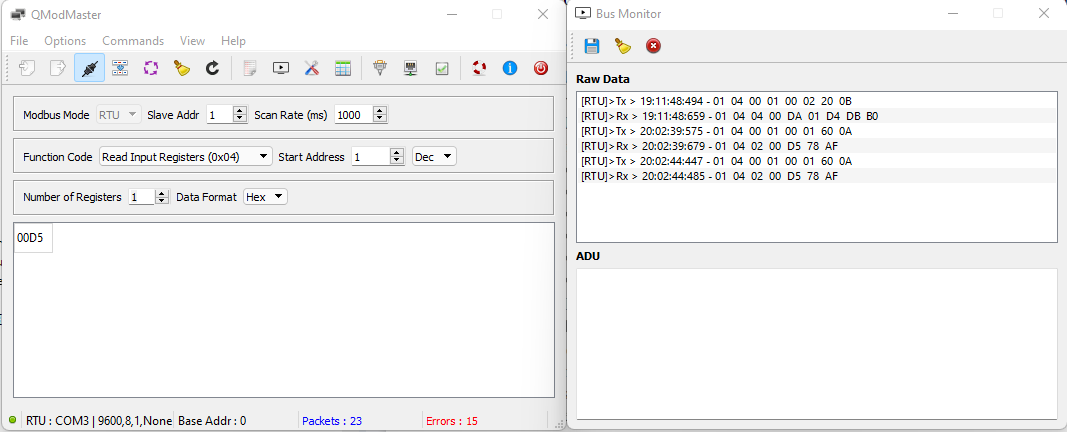
\includegraphics[width=1\columnwidth]{Pictures/modbus-trace.png}}
\caption{QModMaster avec trace des messages}
\label{fig-qmodmaster}
\end{figure}

Pour que le primaire puisse se connecter au secondaire, en plus du nom du port série (ici \texttt{COM3}), il faut disposer de plusieurs informations que l'on peut retrouver dans sa documentation :

\begin{itemize}
    \item la vitesse de transmission sur le bus (ici 9~600 bit/s) et le codage des caractères transmis (ici 8 bits sans bit de parité et un bit de stop)\footnote{\url{https://en.wikipedia.org/wiki/8-N-1}}.
    \item l'adresse du secondaire sur le bus.
\end{itemize}

    \vspace{1em}

La documentation donne également la nature des registres et leur codage. Le tableau~\vref{tab-XY-IR} reprend la définiton des \textit{Input Registers}. Il s'agit de registres qui ne peuvent qu'être lus. La spécification indique que la température est stockée dans le registre 1 sur une longueur de 2 octets, soit l'intégralité de celui-ci.

\begin{table}
\begin{center}
\begin{tabular}{|c|c|c|c|}
\hline
 \rowcolor{purple!10} Register Type & Register Address & Register Contents & Bytes \\ \hline \hline
 \multirow{2}{*}{Input register} & 0x0001 & Temperature & 2 \\ \cline{2-4}
                                 & 0x0002 & Humidity & 2 \\  \hline
\end{tabular}
\end{center}
\caption{Input Register d'un XY-MD02}
\label{tab-XY-IR}
\end{table}

    \vspace{1em}

La documentation indique que le secondaire a l'adresse 0x01 sur le bus RS-485. Il ne reste plus qu'à y envoyer une requête Modbus pour lire ce registre. La fenêtre de trace à droite sur la figure~\vref{fig-qmodmaster} donne les échanges. Nous allons analyser les deux dernières lignes. La première indique le contenu de la requête et la dernière la réponse du secondaire~:

\begin{termc}[backgroundcolor=\color{backcolour}, escapechar=@]
@\texttt{01 \textcolor{blue}{04} \textcolor{purple}{00 01} \textcolor{green!60!black}{00 01} \textcolor{black!30}{60 0A}}@
@\texttt{01 \textcolor{blue}{04} \textcolor{orange}{02} \textbf{00 D5} \textcolor{black!30}{78 AF}}@
\end{termc}

La requête commence par l'adresse du secondaire (\texttt{01}), puis par l'action (\texttt{\textcolor{blue}{04}}) pour lire un \textit{Input Register}, suivit de l'adresse du registre (\texttt{\textcolor{purple}{00 01}}) et du nombre de registres à lire (\textcolor{green!60!black}{00 01}). La requête se termine par la \ac{CRC} validant l'intégrité de la trame (\texttt{\textcolor{black!30}{60 0A}}).

la réponse contient également l'adresse du secondaire (\texttt{01}) et l'action, suivi de la taille de la réponse en octets (\texttt{\textcolor{orange}{02}}) et du résultat demandé (\texttt{\textbf{00 D5}}). 

\Question{Humidité}
{En regardant les échanges de la figure~\vref{fig-qmodmaster} quelle est la valeur mesurée pour l'humidité ?}
{Seul le premier échange demande la lecture de 2 registres à partir du registre ayant l'adresse 0x0001. Dans la réponse on obtient la valeur des deux registres consécutif (\texttt{00 DA} et \texttt{01 D4}). Le tableau~\vref{tab-XY-IR} indique que l'humidité est le second registre, on a donc \texttt{01 D4}.}

Reste à pouvoir interpréter cette valeur. La documentation indique que la valeur est en dixièmes de degrés et que l'unité est le Celsius. En convertissant \texttt{\textbf{00 D5}} en décimal, on obtient 213, soit 21.3\textcelsius.

\Question{Évolution des températures}
{En regardant les échanges de la figure~\vref{fig-qmodmaster} quelle est l'évolution de la température au cours du temps ?}
{On trouve 3 valeurs mesurées à 19:11:48, 20:02:39 et 20:02:44~: \texttt{00 DA}, \texttt{00 D5} et \texttt{00 D5}. Soit 21.8\textcelsius, 21.3\textcelsius ~~et 21.3\textcelsius.}

En résumé, on voit qu'il serait très difficile de faire fonctionner l'équipement sans documentation pour connaître : la vitesse du bus RS-485, l'adresse du secondaire, les adresses des registres utilisés et leur contenu et le codage de l'information dans les registres et les unités utilisées. On a donc un degrés d'interopérabilité faible, les deux entités doivent s'accorder sur un grand nombre de paramètres.

\Question{Taux d'Humidité}
{Quel est le taux d'humidité au moment de la mesure ? La documentation précise qu'il s'agit d'un pourcentage avec une précision au dizième de pourcent. }
{On avait lu la valeur \texttt{01 D4} dans le registre 0x02, soit 468 en décimal. D'où un taux d'humidité de 46.8\%}
    \vspace{1em}

On a pu communiquer avec l'objet en utilisant les paramètres par défaut. Mais pour l'insérer dans un bus, il faut pouvoir modifier certains paramètres. La vitesse de transmission et le codage des octets doit être le même, des secondaires ne peuvent pas avoir la même adresses sur le bus.
Le XY-MD02 dispose aussi de \textit{holding register} permettant de le paramétrage comme le montre la table~\vref{tab-XY-HR}


\begin{table}
\begin{center}
\begin{tabular}{|c|c|c|c|}
\hline
 \rowcolor{purple!10} Register Type & Register Address & Register Contents & Bytes \\ \hline \hline
 \multirow{9}{*}{Holding register} & 0x0101 & Device Address & 2 \\ \cline{2-4}
                                 & 0x1202 & Bit rate: & 2 \\
                                 &        & \tabitem 0~: 9600  & \\
                                 &        & \tabitem 1~: 14400 & \\
                                 &        & \tabitem 2~: 19200 & \\  \cline{2-4}
                                 & 0x0103 & Temperature correction & 2 \\ 
                                 &         & -10\textcelsius ~~- 10\textcelsius &  \\ \cline{2-4}
                                 & 0x0104 & Humidity correction & 2 \\ 
                                 &         & -10\%RH - 10\%RH &  \\ \hline
\end{tabular}
\end{center}
\caption{Holding Register d'un XY-MD02}
\label{tab-XY-HR}
\end{table}

\subsection{Passerelle IP}

\begin{wrapfigure}{r}{8cm}
\centerline{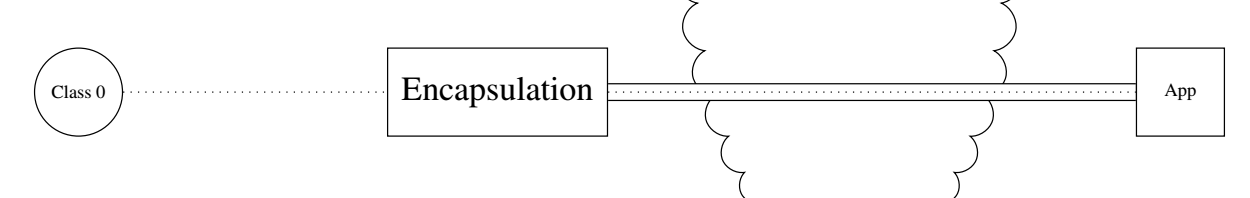
\includegraphics[width=.5\columnwidth]{Pictures/encaps3.png}}
\end{wrapfigure}

Il est possible d'étendre la portée d'un réseau Modbus en ajoutant une passerelle IP. Cela correspond au troisième méthode d'interconnexion de la figure~\vref{fig-encap}. La passerelle, connectée sur le bus où restent connectés les secondaires, possède une adresse IP. Le primaire ouvre une connexion TCP avec la passerelle et y envoie ses requêtes. La passerelle recopie les données sur le bus. Inversement, les réponses des objets sont retournées à la passerelle qui les envoie au primaire en utilisation la connexion TCP. La figure~\vref{fig-gwmodbus} illustre les échanges. On note l'ouverture de connexion TCP qui se fait au démarrage du primaire qui reste active pour toute les échanges. On peut aussi remarquer que les messages TCP sont acquittés. La figure~\vref{fig-msg-modbus} montre les champs commun aux format sur le bus RS-485 et dans des paquets IP.


\begin{figure}
    \centering
    
    \begin{tikzpicture}
    
    %\clip (0.0, 0) rectangle (16,10);
    %\draw[help lines] (0,0) grid (15,9); 
    
    \node[inner sep=0pt] (meter) at (1,7)
        {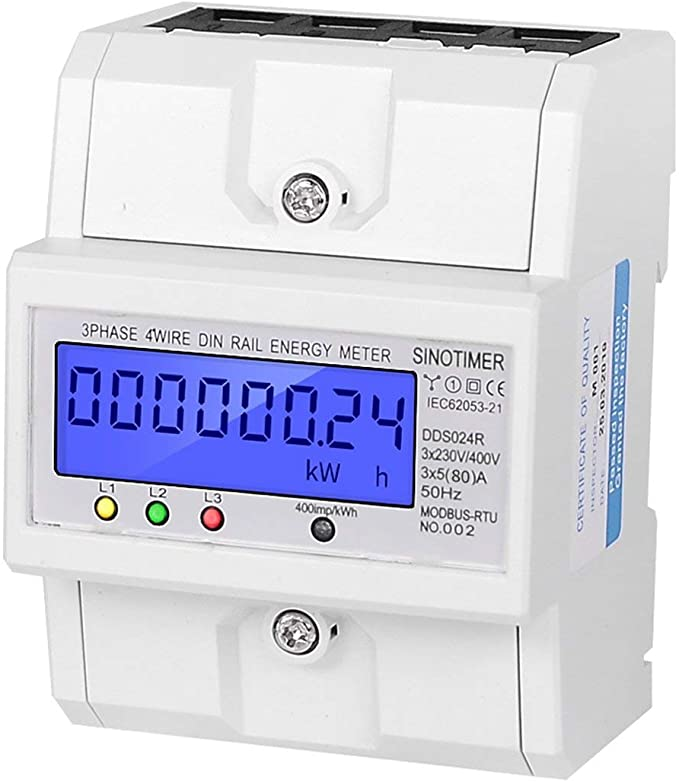
\includegraphics[width=.1\textwidth]{meter.jpg}};
        
    \node[inner sep=0pt] (gw) at (7,7)
        {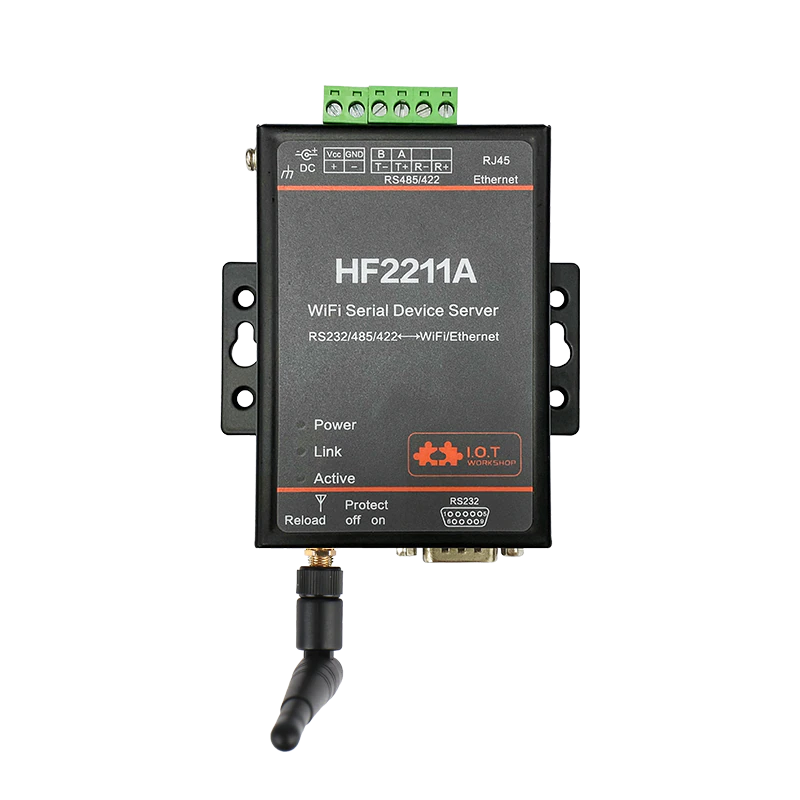
\includegraphics[width=.2\textwidth]{modbusGW2.png}};
    
    \node[inner sep=0pt] (primary) at (13,7)
        {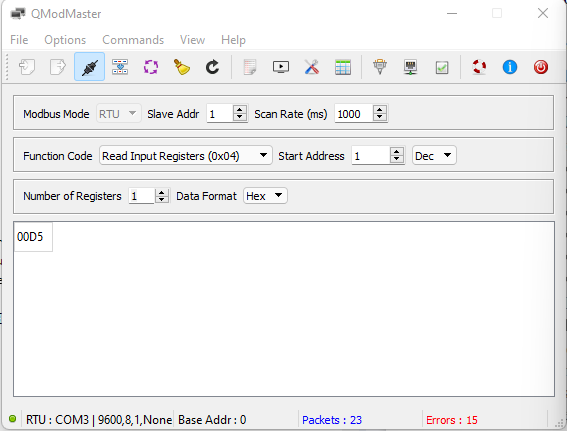
\includegraphics[width=.2\textwidth]{Pictures/QModMaster.png}};
        
        
    \coordinate (tline) at (0, 5.4);
    
    \draw (meter |- tline) node {\small{Compteur}};
    \draw (gw |- tline) node {\small{Passerelle}};
    \draw (primary |- tline) node {\small{Primaire}};
    
    \coordinate (wline) at (0, 8.3);
    
    \draw [decorate, decoration=snake, blue] (meter |- wline) -- coordinate(a)  (gw |- wline);
%    \draw [decorate, decoration={snake}, mirror, yellow] (gw |- wline) -- coordinate(a) (meter);
    
    \draw (a) node [below] {\small{RS-485}};
    
    \path(gw) -- coordinate(b) (primary);
    
    \draw [very thick] ([xshift=0.2cm]gw |- wline) -- coordinate(c) (primary |- wline);
     \draw (c) node [below] {\small{Internet}};
     
     \coordinate(cline) at (0, 5);
     
     \draw [->, thin] (meter |- cline) -- ++ (0, -4) ;
     \draw [->, thin] (gw |- cline) -- ++ (0, -4);
     \draw [->, thin] (primary |- cline) -- ++ (0, -4); 
     
     \draw [thick, ->] ([yshift=-0.1cm] primary |- cline) coordinate (d) -- ([yshift=-0.3cm] gw |- cline) coordinate (e);
     
     \draw (d) node [right] {\tiny{SYN}};
     \draw (e) node [left] {\tiny{SYN/ACK}};
     \draw [thick, ->] (e) -- ([yshift=-0.5cm] primary |- cline) coordinate (f);
     
    \draw (f) node [right] {\tiny{ACK}};
    \draw [thick, ->] (f) -- ([yshift=-0.7cm] gw |- cline) coordinate (h);
    
    \coordinate (tcp_line) at (14.5, 0);
    
    \draw [decoration=brace, decorate] (d -| tcp_line) -- coordinate(i) (h -| tcp_line);
    
    \draw (i) node [below, rotate=90] {\small{Ouverture}};
    
    \draw [double, double distance=0.2cm,] ([yshift=-1.5cm] primary |- cline) coordinate (d) -- ([yshift=-1.7cm] gw |- cline) coordinate (e);
    
    
    \draw  [->] ([yshift=-1.8cm] gw |- cline) -- ([yshift=-2cm] primary |- cline) coordinate(k);
    \draw (k) node [right] {\tiny{ACK}};


    \draw [purple, -> ] ([yshift=-1.5cm] primary |- cline) coordinate (d) -- ([yshift=-1.7cm] gw |- cline);      
    \draw [purple, -> ] ([yshift=-1.7cm] gw |- cline)  -- ([yshift=-2.1cm] meter |- cline) coordinate (e);  

    \draw (d) node [right,purple] {\small{requête}};

    \draw [blue, ] (e) -- ([yshift=-2.5cm] gw |- cline);    
    \draw [double, double distance=0.2cm ] ([yshift=-2.5cm] gw |- cline) -- ([yshift=-2.7cm] primary |- cline);    
    \draw [blue, -> ] ([yshift=-2.5cm] gw |- cline) -- ([yshift=-2.7cm] primary |- cline) coordinate(m);   
    
    \draw  [->] ([yshift=-2.8cm] primary |- cline) -- ([yshift=-3cm] gw |- cline) coordinate(l);
    \draw (l) node [left] {\tiny{ACK}};
    
    \draw (m) node [right,blue] {\small{réponse}};

   
    \end{tikzpicture}
    
    \caption{Passerelle entre le réseau Internet et Modbus.}
    
    \label{fig-gwmodbus}
\end{figure}

\begin{figure}
    \centering
    
    \begin{tikzpicture}
    
  
    
    
    
    \draw (0,0) node (tid) [rectangle, draw,  minimum width = 2cm, minimum height = 0.5cm, fill=olive!50 ] {};
    \draw (tid) node {\tiny{Transaction ID}};


    \draw (tid.east) node (pid) [right, rectangle, draw,  minimum width = 2cm, minimum height = 0.5cm, fill=olive!50 ] {};
    \draw (pid) node {\tiny{Protocol ID}};

    \draw (pid.east) node (len) [right, rectangle, draw,  minimum width = 2cm, minimum height = 0.5cm, fill=olive!50 ] {};
    \draw (len) node {\tiny{Length}};
    
    \draw (len.east) node (uid) [right, rectangle, draw,  minimum width = 1cm, minimum height = 0.5cm, fill=olive!50 ] {};
    \draw (uid) node {\tiny{Unit ID}};

    \draw (uid.east) node (fcode) [right, rectangle, draw,  minimum width = 1cm, minimum height = 0.5cm, fill=green!50 ] {};
    \draw (fcode) node {\tiny{FCode}};
    
    \draw (fcode.east) node (data) [right, rectangle, draw,  minimum width = 4cm, minimum height = 0.5cm, fill=green!50 ] {};
    \draw (data) node {\tiny{Data}};
    
    \draw [green!50] (data.north) -- +(-1, 0) -- +(1, 0);
    \draw [green!50] (data.south) -- +(-1, 0) -- +(1, 0);
    \draw [dashed] (data.north) -- +(-1, 0) -- +(1, 0);
    \draw [dashed] (data.south) -- +(-1, 0) -- +(1, 0);
    
    \draw (data.east) node [right] {\small{TCP}};
    
    
    \path (uid.west) -- ++(0, 1.5) coordinate(x);
    \draw (x) node (addr) [right, rectangle, draw,  minimum width = 1cm, minimum height = 0.5cm, fill=olive!50 ] {};
    \draw (addr) node {\tiny{Addr}};  

   \draw (addr.east) node (fcode) [right, rectangle, draw,  minimum width = 1cm, minimum height = 0.5cm, fill=green!50 ] {};
    \draw (fcode) node {\tiny{FCode}};
    
    \draw (fcode.east) node (data) [right, rectangle, draw,  minimum width = 4cm, minimum height = 0.5cm, fill=green!50 ] {};
    \draw (data) node {\tiny{Data}};    
   \draw [green!50] (data.north) -- +(-1, 0) -- +(1, 0);
    \draw [green!50] (data.south) -- +(-1, 0) -- +(1, 0);
    \draw [dashed] (data.north) -- +(-1, 0) -- +(1, 0);
    \draw [dashed] (data.south) -- +(-1, 0) -- +(1, 0);
    

    \draw (data.east) node (crc) [right, rectangle, draw,  minimum width = 2cm, minimum height = 0.5cm, fill=blue!50 ] {};
    \draw (crc) node {\tiny{CRC}};
    
    \draw(x) node [left] {\small{RS-385}};
    \end{tikzpicture}
    
    \caption{Messages Modbus sur bus RS-485 et sur IP/TCP}
    
    \label{fig-msg-modbus}
\end{figure}


Comme dans l'exemple précédent du capteur de température, les spécifications du \Index{compteur électrique} sont nécessaires pour comprendre la signification des registres utilisables. Le compteur code ses valeurs sur des nombres flottant sur 32 bits dont le codage est spécifié par la norme \Index{IEEE 754}\footnote{\url{https://en.wikipedia.org/wiki/IEEE_754}}. Ces valeurs sur 32 bits doivent être codées sur deux registres consécutifs d'où l'incrémentation de 2 en 2 que l'on retrouve sur la tableau~\vref{tab-meter-IR}, le compteur pouvant mesurer trois phase électriques.


\begin{table}
\begin{center}
\begin{tabular}{|c|c|c|c|c|}
\hline
 \rowcolor{purple!10} Register Type & Register Address & Register Contents & Unité & Format \\ \hline \hline
 \multirow{10}{*}{Input register} & 0x0000 & \Index{Voltage} phase A & V &  IEEE 754 \\ \cline{2-5}
                                 & 0x0002 & Voltage phase B & V &  IEEE 754 \\ \cline{2-5}
                                 & 0x0004 & Voltage phase C & V &  IEEE 754 \\ \cline{2-5}
                                 & 0x0008 & \Index{Intensité} phase A & A &  IEEE 754 \\ \cline{2-5}
                                 & 0x000A & Intensité phase B & A &  IEEE 754 \\ \cline{2-5}
                                 & 0x000C & Intensité phase C & A &  IEEE 754 \\ \cline{2-5}
                                 & 0x0010 & \Index{Puissance} Totale & KWh &  IEEE 754 \\ \cline{2-5}
                                 & 0x0012 & Puissance phase A & KWh &  IEEE 754 \\ \cline{2-5}
                                 & 0x0014 & Puissance phase B & KWh &  IEEE 754 \\ \cline{2-5}
                                 & 0x0016 & Puissance phase C & KWh &  IEEE 754 \\ \cline{2-5}
                                 & 0x0036 & \Index{Fréquence} & Hz &  IEEE 754 \\ \hline

\end{tabular}
\end{center}
\caption{quelques \textit{Input Register} du compteur électrique}
\label{tab-meter-IR}
\end{table}

    \vspace{1em}

\Index{Wireshark} peut capturer une requête ayant circulé sur le réseau Ethernet, coté primaire (cf. figure~\vref{fig-modbus-ws}).

\begin{figure}[tbp]
\centerline{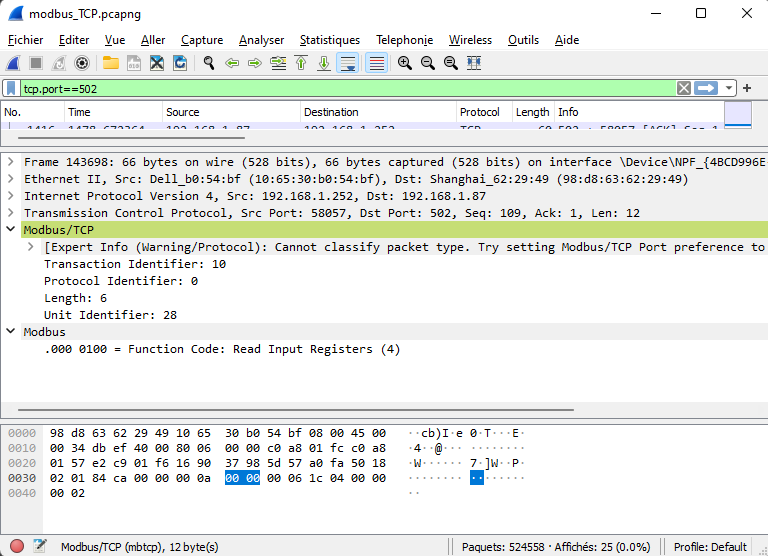
\includegraphics[width=1\columnwidth]{Pictures/modbus-ws.png}}
\caption{Capture avec \Index{Wireshark} d'une trame contenant un message Modbus.}
\label{fig-modbus-ws}
\end{figure}


\begin{termc}[backgroundcolor=\color{backcolour}, escapechar=#]
#\texttt{\small{0000 \colorbox{purple!50}{98 d8 63 62 29 49 10 65 30 b0 54 bf 08 00}\colorbox{blue!30}{45 00}   ..cb)I.e0.T...E.}}#
#\texttt{\small{0010  \colorbox{blue!30}{00 34 db ef 40 00 80 06 00 00 c0 a8 01 fc c0 a8}   .4..@...........}}#
#\texttt{\small{0020  \colorbox{blue!30}{01 57}\colorbox{red!30}{e2 c9 01 f6 16 90 37 98 5d 57 a0 fa 50 18}   .W......7.]W..P.}}#
#\texttt{\small{0030  \colorbox{red!30}{02 01 84 ca 00 00} \ul{00 0a} \ul{00 00} \ul{00 06} 1c \textcolor{blue}{04} \textcolor{red}{00 00}   ................}}#
#\texttt{\small{0040  \textcolor{green}{00 02}   ..              }}#                                 
\end{termc}

On retrouve les encapsulations des protocoles Ethernet, IP et TCP, suivi des données TCP. Elles se composent de  trois champs qui n'existent pas dans la requête circulant sur le bus RS-485~:
\begin{itemize}
    \item le numéro de la transaction sur deux octets incrémenté à chaque requête,
    \item la version du protocole sur deux octets, 
    \item la longueur en octet de la transaction.
\end{itemize}

    \vspace{1em}

Les champs suivants sont identiques à ceux de la trame sur le bus RS-485~:
\begin{itemize}
    \item l'adresse du secondaire sur un octet, ici 0x1c ou 28,
    \item la nature de la requête : 0x04 pour lire un input register,
    \item le registre à lire sur deux octets, ici 0x0000 correspondant à la tension sur la phase A.
    \item le nombre de registre à lire, ici 2 pour obtenir les 32 bits de la valeur.
\end{itemize}

    \vspace{1em}

Le primaire reçoit la réponse suivante~:

\begin{termc}[backgroundcolor=\color{backcolour}, escapechar=#]
#\texttt{\small{0000  \colorbox{purple!50}{10 65 30 b0 54 bf 98 d8 63 62 29 49 08 00}\colorbox{blue!30}{45 00}   .e0.T...cb)I..E.}}# 
#\texttt{\small{0010  \colorbox{blue!30}{00 35 c9 75 00 00 40 06 2c aa c0 a8 01 57 c0 a8}   .5.u..@.,....W..}}# 
#\texttt{\small{0020  \colorbox{blue!30}{01 fc}\colorbox{red!30}{01 f6 e2 c9 5d 57 a0 fa 16 90 37 a4 50 18}   ......]W....7.P.}}# 
#\texttt{\small{0030  \colorbox{red!30}{44 70 e1 6e 00 00} \ul{00 0a} \ul{00 00} \ul{00 07} 1c \textcolor{blue}{04} \textcolor{orange}{04}\colorbox{black}{\textcolor{white}{43}}   Dp.n...........C}}# 
#\texttt{\small{0040  \colorbox{black}{\textcolor{white}{69 9e 4a}} \ \ \ \ \ \ \ \ \ \ \ \ \ \ \ \ \ \ \ \ \ \ \ \ \ \ \ \ \ \ \ \ \ \ \ \ \ \ \ i.J}}# 
                           
\end{termc}

On y retrouve, après les encapsulations protocolaires d'Ethernet, IP et TCP les données suivantes~:
\begin{itemize}
    \item le numéro de transaction qui correspond à celui employé dans la requête précédente. cela permet de faire le lien entre les deux messages qui aurait pu se defaire en cas de perte de paquets sur le réseau Internet,
    \item la version du protocole,
    \item la longueur de la réponse, ici 7 octets,
    \item l'adresse du secondaire ayant répondu, ici 28,
    \item la nature de la requête,
    \item le nombre d'octets retournés, ici 4,
    \item et la valeur des deux registres \texttt{0x43699e4a} qui correspond à un nombre flottant tel que le représente le standard IEEE 754. Il existe de nombreux sites sur Internet qui permettent la conversion\footnote{\url{https://www.h-schmidt.net/FloatConverter/IEEE754.html}}. Comme le montre la figure~\vref{fig-ieee754}, on obtient la valeur \SI{233.61831665}\volt qui correspond bien à une tension offerte par un réseau électrique.
\end{itemize}

  \begin{figure}[tbp]
\centerline{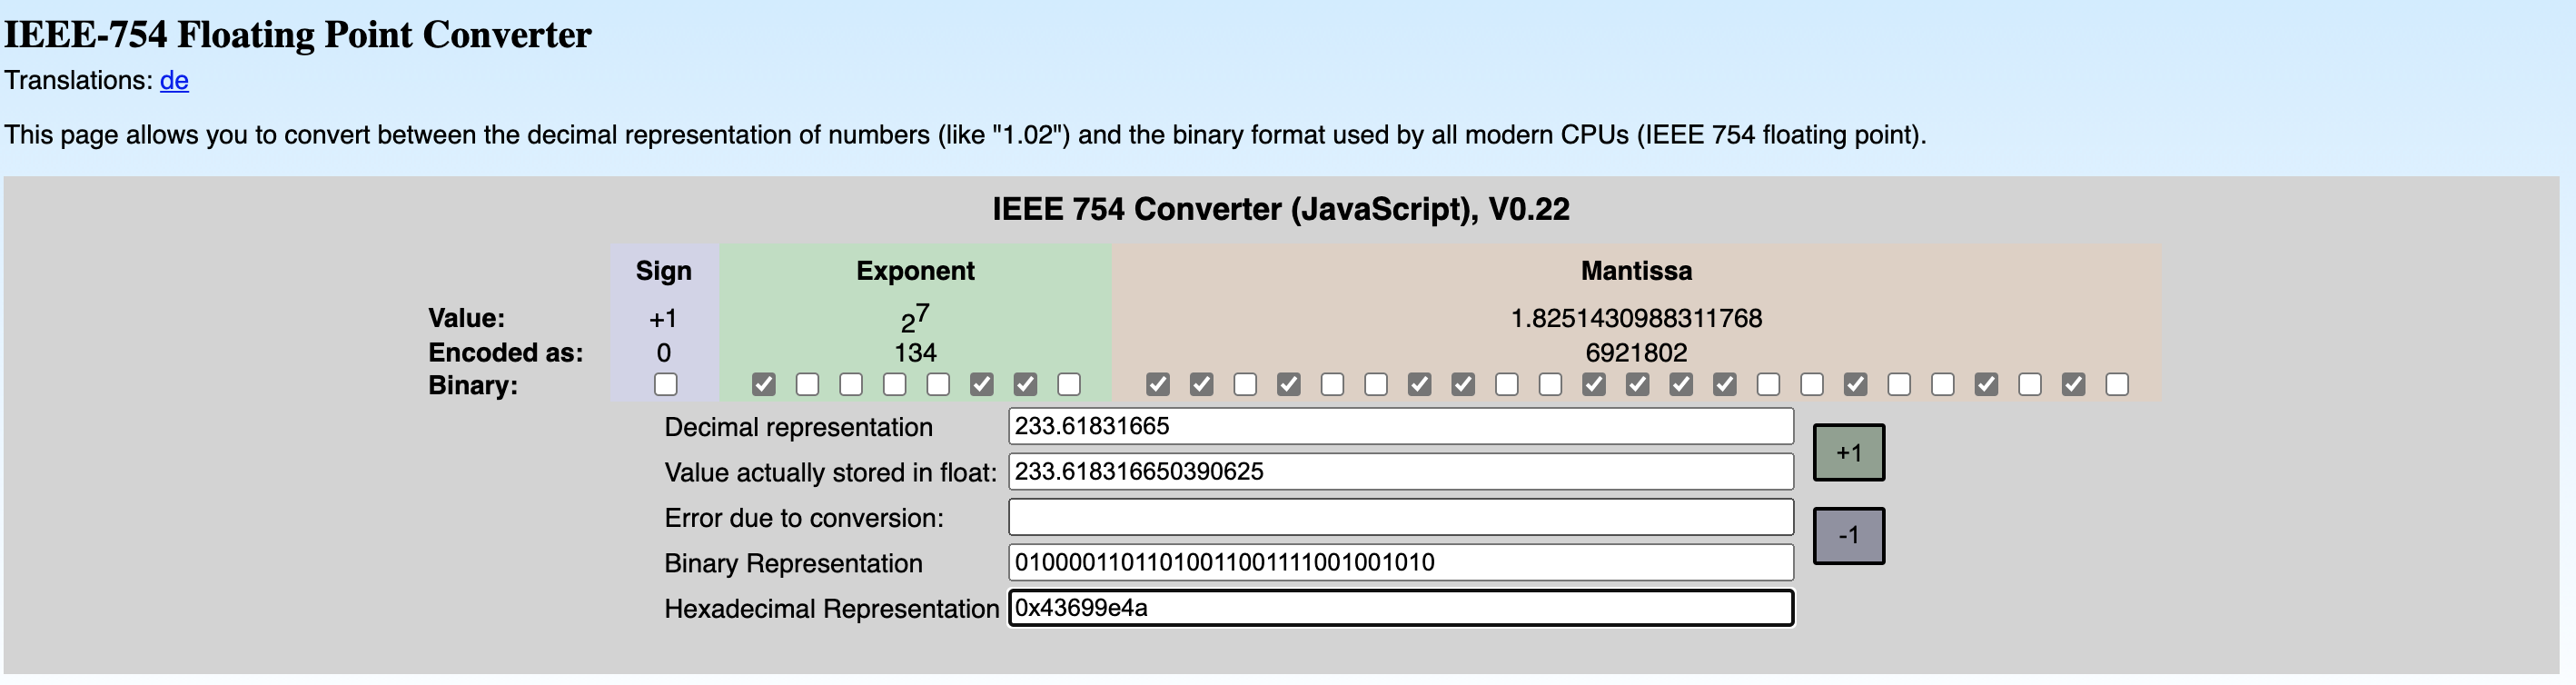
\includegraphics[width=1\columnwidth]{Pictures/IEEE754.png}}
\caption{Conversion d'un nombre flottant}
\label{fig-ieee754}
\end{figure}

\Question{Requête Modbus TCP}
{Soit l'échange donné figure~\vref{fig-exo-ws} correspondant à une requête Modbus et à une réponse.
Quel est le numéro de port utilisé par Modbus TCP.}
{Il y a deux ports dasn l'en-tête TCP, mais comme il s'agit d'une requête, il faut prendre le port destination~:0x1f6, soit 502 en décimal}

\Question{Requête Modbus TCP}
{En poursuivant l'analyse du trafic, quelle valeur de registre est demandée.}
{Le registre 0x36 est demandé, en regardant dans la table~\vref{tab-meter-IR}, il s'agit de la fréquence en Hz}

\Question{Réponse Modbus TCP}
{En analysant le paquet suivant, 
Comment peut-on vérifier que la réponse peut correspondre à la requête précédente.}
{Le numéro de séquence 0x000c est le même dans les deux trames.}


\Question{Réponse Modbus TCP}
{Quelle valeur est retournée. Est-ce cohérent ?}
{La valeur du registre est 0x4247e95b correspond à un nombre flottant IEEE 754, en convertissant on obtient la valeur 49.9778862 Hz qui est très proche de la fréquence du réseau électrique européen.}

\begin{figure}[tbp]

\begin{termc}[backgroundcolor=\color{backcolour}, escapechar=#]
#\texttt{\small{0000  \colorbox{purple!50}{98 d8 63 62 29 49 10 65 30 b0 54 bf 08 00}\colorbox{blue!30}{45 00}   ..cb)I.e0.T...E.}}#
#\texttt{\small{0010  \colorbox{blue!30}{00 34 db f3 40 00 80 06 00 00 c0 a8 01 fc c0 a8}   .4..@...........}}#
#\texttt{\small{0020  \colorbox{blue!30}{01 57}\colorbox{red!30}{e2 c9 01 f6 16 90 37 b0 5d 57 a1 14 50 18}   .W......7.]W..P.}}#
#\texttt{\small{0030  \colorbox{red!30}{02 01 84 ca 00 00} 00 0c 00 00 00 06 1c 04 00 36   ...............6}}#
#\texttt{\small{0040  00 02 \ \ \ \ \ \ \ \ \ \ \ \ \ \ \ \ \ \ \ \ \ \ \ \ \ \ \ \ \ \ \ \ \ \ \ \ \ \ \ \ \ \  ..}}#
                           
\end{termc}

\begin{termc}[backgroundcolor=\color{backcolour}, escapechar=#]
#\texttt{\small{0000  \colorbox{purple!50}{10 65 30 b0 54 bf 98 d8 63 62 29 49 08 00}\colorbox{blue!30}{45 00}   .e0.T...cb)I..E.}}#
#\texttt{\small{0010  \colorbox{blue!30}{00 35 8b 15 00 00 40 06 6b 0a c0 a8 01 57 c0 a8}   .5....@.k....W..}}#
#\texttt{\small{0020  \colorbox{blue!30}{01 fc}\colorbox{red!30}{01 f6 e2 c9 5d 57 a1 14 16 90 37 bc 50 18}   ......]W....7.P.}}#
#\texttt{\small{0030  \colorbox{red!30}{44 70 f1 f0 00 00} 00 0c 00 00 00 07 1c 04 04 42   Dp.............B}}#
#\texttt{\small{0040  47 e9 5b \ \ \ \ \ \ \ \ \ \ \ \ \ \ \ \ \ \ \ \ \ \ \ \ \ \ \ \ \ \ \ \ \ \ \ \ \ \ \ \  G.[}}#
                           
\end{termc}
\caption{Capture à étudier.}
\label{fig-exo-ws}
\end{figure}
%\chapter{ARCHITECTURE POUR L'IOT}

\section{Introduction}
  
    \vspace{1em}
   
 \begin{wrapfigure}{r}{3cm}
\Youtube{https://youtu.be/DjRhnbg0FjY}
\end{wrapfigure}

Les objets se caractérisent 
par 
une capacité
de traitement limitée et par une consommation énergétique réduite pour préserver l’autonomie imposée par une alimentation sur batterie.
Or, les activités les plus consommatrices pour un équipement sont l’émission et la réception de données. 
Pour maximiser l’autonomie des équipements, il faut revoir l’intégralité des protocoles, mais en les calquant sur les architectures existantes pour en assurer la compatibilité. 

La figure~\vref{fig-pile-IoT} reprend un certain nombre d'adaptation protocolaires, à différents niveau du modèle \ac{ISO}, capable de s'adapter aux caractéristiques des objets contraints. Dans les chapitres suivants nous reviendrons sur ces technologies en partant de la représentation des données pour aller jusqu'aux couches basses.

\begin{figure}[tbp]
\centerline{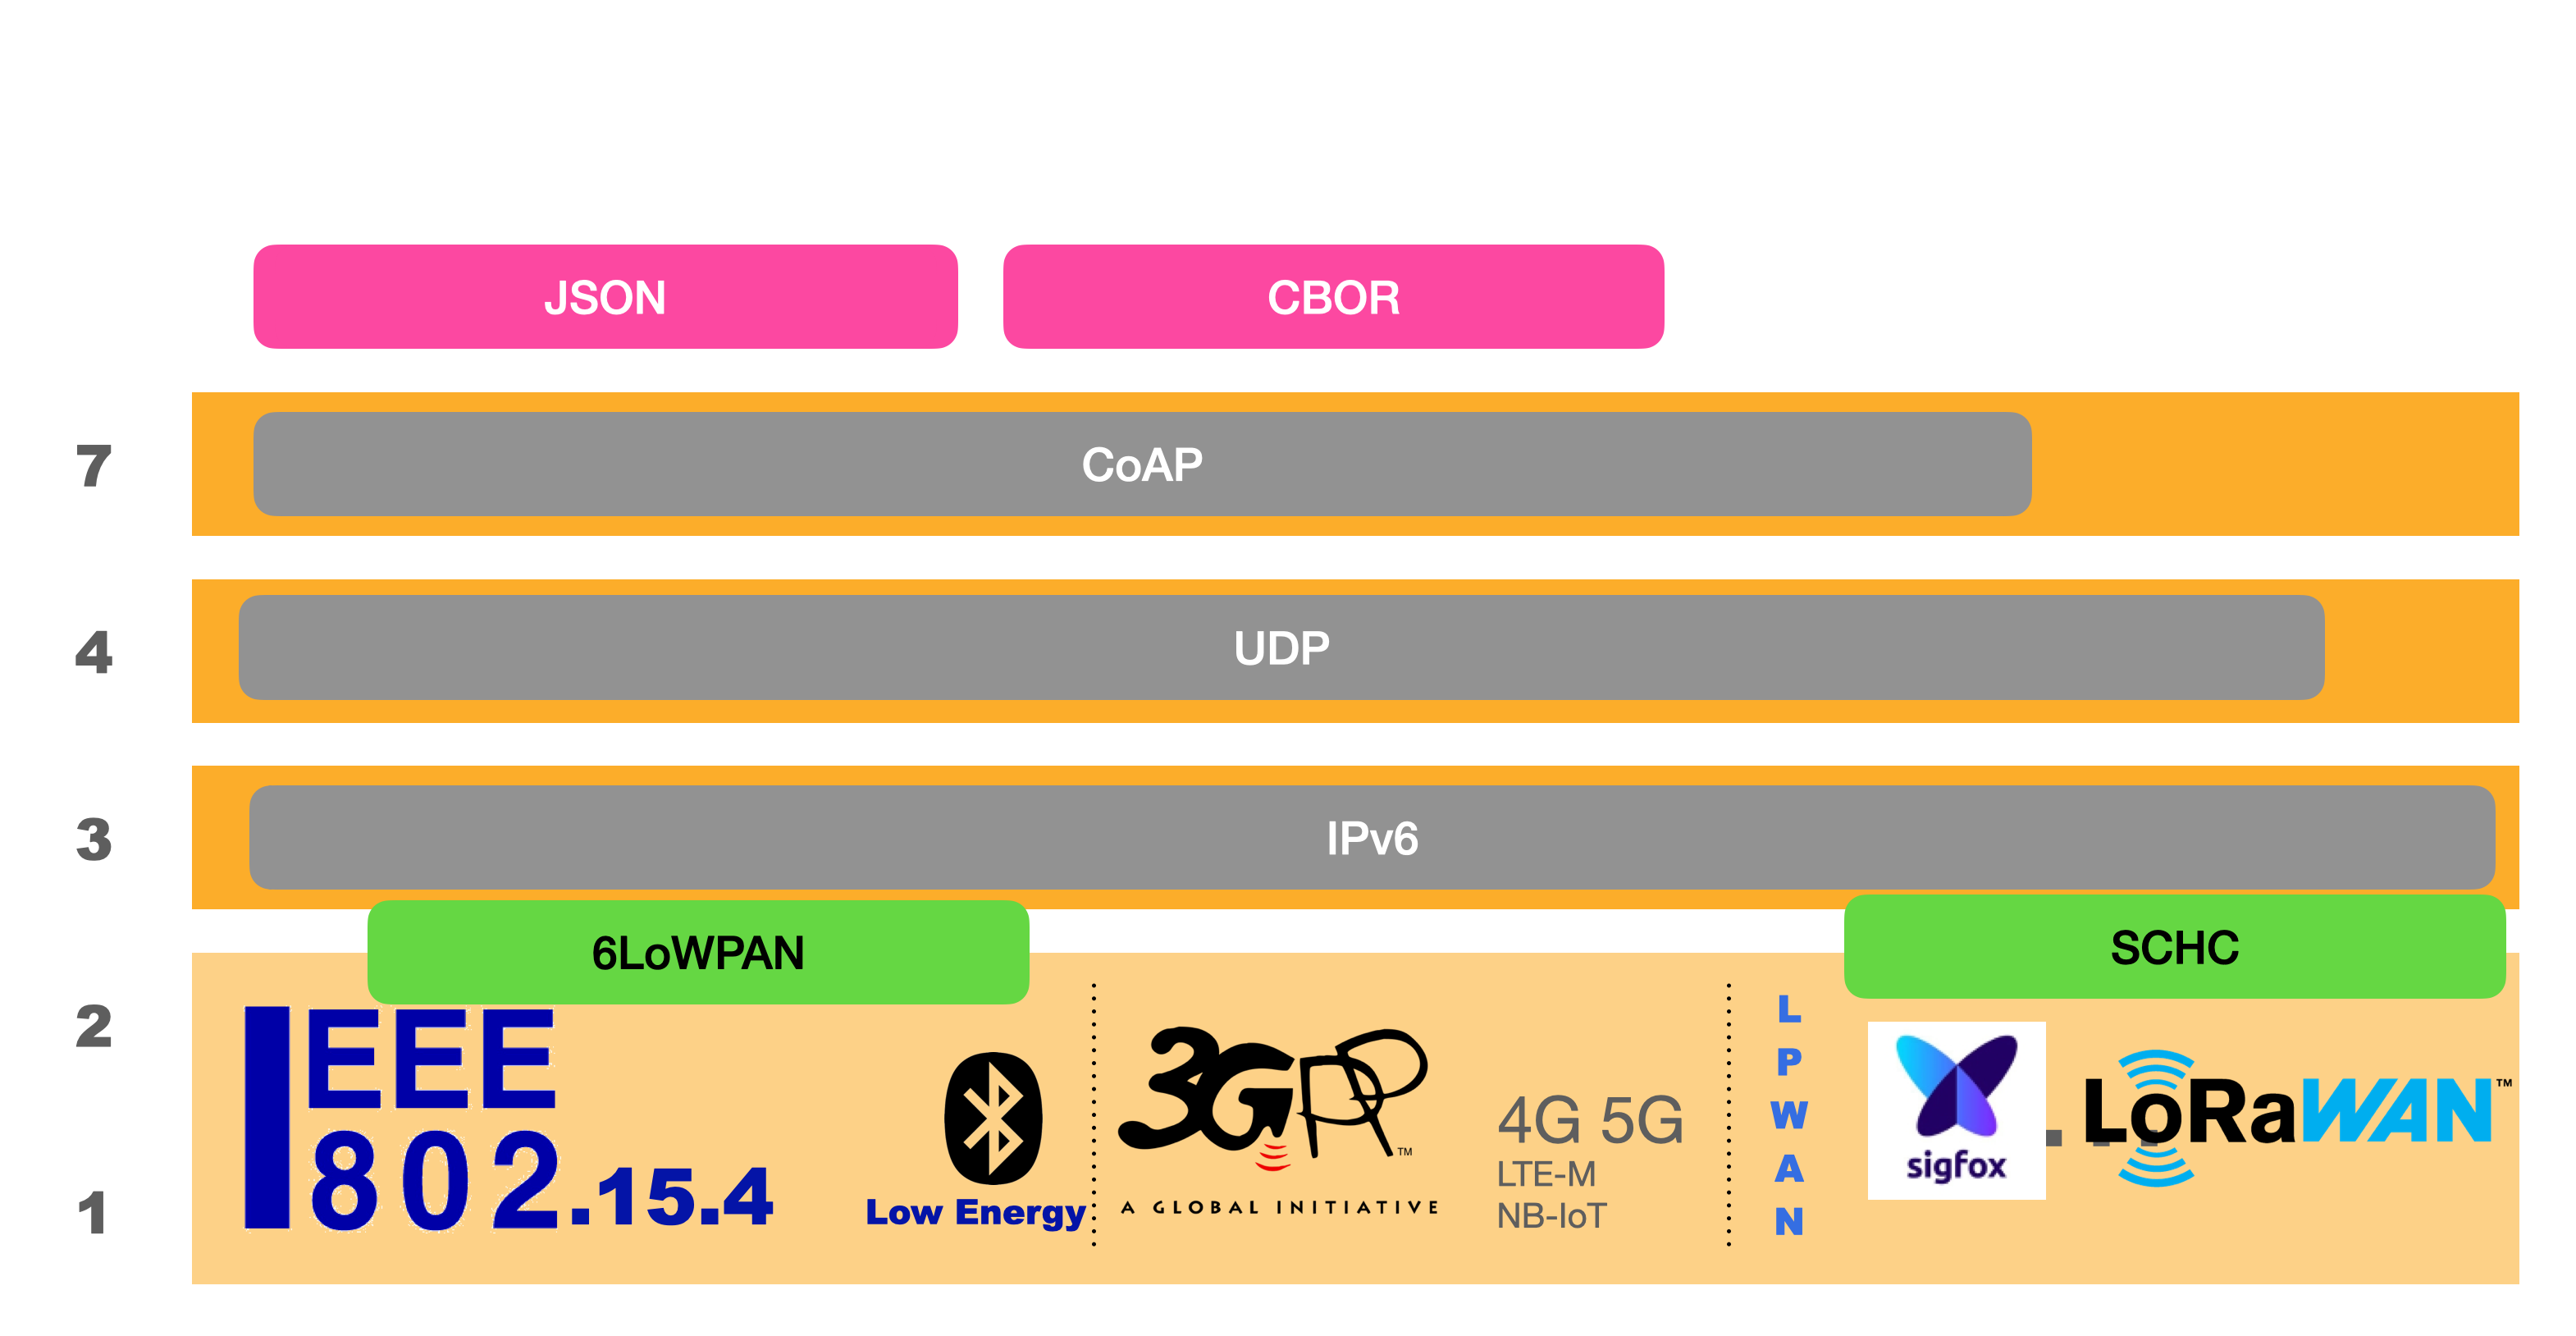
\includegraphics[width=1\columnwidth]{Pictures/Capture17.png}}
\caption{Pile protocolaire de l'IoT}
\label{fig-pile-IoT}
\end{figure}

\section{Topologies}

Les réseaux pour l’internet des objets peuvent être divisés en deux catégories : les topologies \Index{maillé}es (\Index{Mesh} in english) et étoilées (\Index{star}).


\subsection*{Réseaux Maillés}

Les réseaux maillés, tels que la famille IEEE 802.15.4,  sont une adaptation d’un protocole d’accès Wi-Fi pour préserver l’énergie. La portée de transmission est limitée à 50 mètres pour limiter la consommation d'énergie ; et par conséquent les messages doivent être relayés par d’autres nœuds pour atteindre leur destination.

Le débit est de quelques centaines de kilobits/s et la taille de la trame est de quelques centaines d’octets. 

Ces réseaux sont performants pour transporter des données IoT, mais le protocole de routage, ainsi que le relayage des trames, consomment l’énergie des objets.

\subsection*{Réseaux en Étoile}\label{chap-star}

Les topologies en \Index{étoile} ne nécessitent pas de tels mécanismes de routage. Toutes les communications se font avec un point central qui relaie les informations vers la destination.

Les progrès réalisés dans le traitement des signaux permettent d’étendre la portée de transmission à faible puissance. Cette famille de réseaux est appelée réseaux étendus à faible puissance (\ac{LPWAN}) comme \Index{Sigfox}, \Index{LoRaWAN}, ou même du côté de la téléphonie cellulaire avec des évolutions de la norme \Index{4G} et une intégration plus complète dans la \Index{5G}. Le \rfc{8376} donne, en anglais, un aperçu de ces techniques.


    \vspace{1em}

Avec une puissance de transmission de 25 mW, il est possible de communiquer sur une distance de 3 km en milieu urbain et de 20 km dans un environnement dégagé. Les \ac{LPWAN} sont compatibles avec les appareils de classe 0 car ils ne nécessitent pas la mise en place d’une pile \ac{IP}. La figure ci-dessous décrit une architecture typique pour les \ac{LPWAN}.

\begin{figure}[tbp]
\centerline{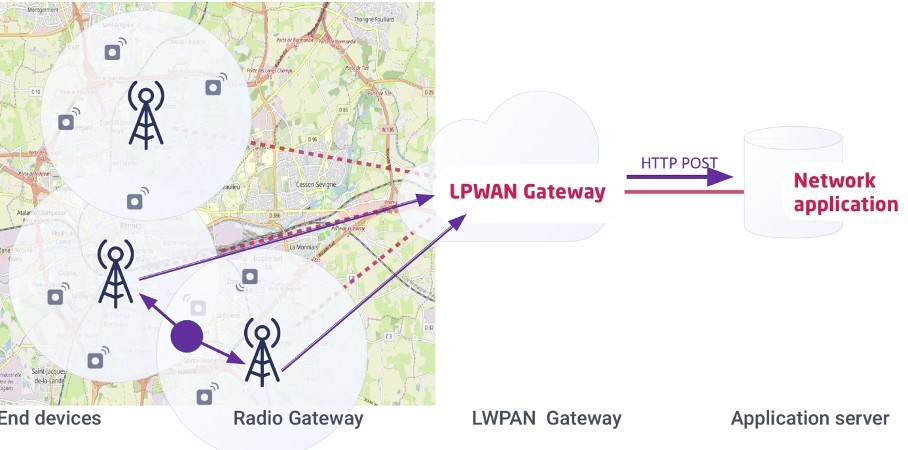
\includegraphics[width=1\columnwidth]{Pictures/TolologieStar.jpg}}
\caption{Architecture simplifiée des réseaux LPWAN}
\label{fig-topo-star}
\end{figure}


L’appareil envoie des données brutes sur le réseau radio. Le signal radio est capté par une ou plusieurs passerelles radio, et la trame est envoyée à une passerelle réseau (\ac{LNS}  pour les réseaux \Index{LoRaWAN}, et \ac{SCEF} pour les réseaux \ac{3GPP}).

Le propriétaire de l’appareil a associé l’appareil à un connecteur dans le LPWAN \ac{NGW} qui peut être un \ac{URI}, une adresse de broker \ac{MQTT} ou une Web socket. Lorsque l’appareil envoie des données, il est relié à l’application par ce tunnel.

    \vspace{1em}


Certaines technologies telles que LoRaWAN ou Sigfox utilisent des bandes sans licence, imposant un cycle d’utilisation (\Index{Duty Cycle}) de 0,1 à 10 \% selon les canaux pour assurer l’équité entre les nœuds, empêchant ainsi qu'un équipement ne monopolise le canal de transmission. Comme cette restriction s’applique également à l’antenne du fournisseur, la communication entre le réseau et l’appareil est considérablement limitée.

L’utilisation principale de ces réseaux \ac{LPWAN} est la télémétrie où un appareil envoie régulièrement des informations ou une alarme de temps en temps (par exemple des capteurs de température). Le débit et la taille des messages est beaucoup plus réduit que dans le cas de réseaux maillés.

    \vspace{1em}

\section{Niveaux 1 et 2}

 Concernant le niveau 2, le but est de gagner en énergie lors des transmissions. Déjà on peut dire adieu à Ethernet car cela imposerait d'utiliser l'infrastructure filaire et donc on ne pourrait pas placer les objets où on veut, surtout s'ils se déplacent. Les communications par ondes radio sont privilégiées. 
 
 Pour l'Internet des objets, le \Index{Wi-Fi} est également trop gourmand en énergie. On lui préfère donc une évolution appelée \Index{IEEE 802.15.4} qui reprend son principe de fonctionnement mais l'adapte à un faible débit et à des trames de petite taille. En particulier pour économiser l'énergie, la portée est réduite à une dizaine de mètres et il faut généralement utiliser des relais pour atteindre une destination. 
 
 \Index{Bluetooth} a été adapté pour des objets avec une basse consommation \ac{BLE}. 
     \vspace{1em}

 Côté téléphonie cellulaire, les protocoles évoluent pour prendre en compte les objets. La norme 4G a intégrée les communications à plus bas débit. La 5G inclura une classe permettant des communications avec les objets économes en énergie et réduisant les temps de latence. 
 
\section{IP et couches d'adaptation}

  Au niveau 3, on va vers l'utilisation plus massive d'\ac{IPv6} puisque la version 4 a son espace d'adressage saturé. la taille de l’adresse est étendue sur 128 bits offrant $2^{96}$ fois plus d’adresses.
  
  \begin{figure}[tbp]
\centerline{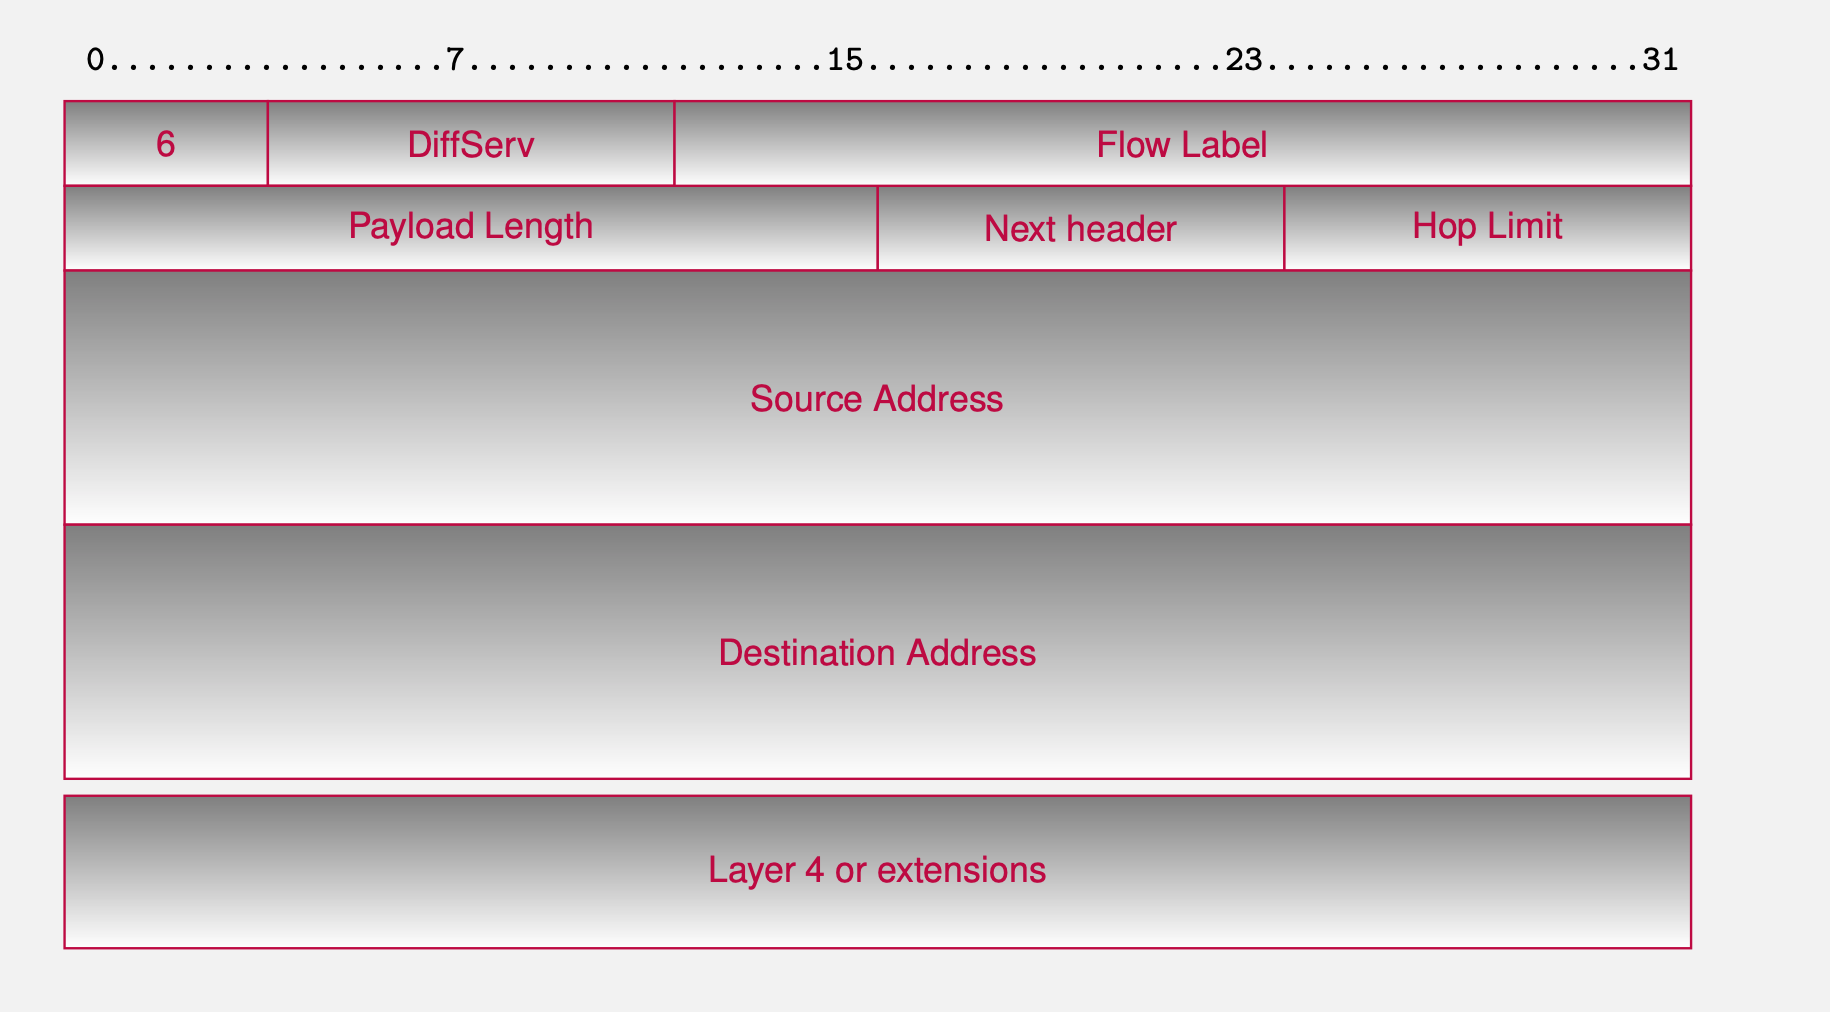
\includegraphics[width=1\columnwidth]{Pictures/Capture18.png}}
\caption{Format d'un en-tête IPv6}
\label{fig-IPv6-header}
\end{figure}

  
  
  
  
  
  Mais, comme on le voir sur la figure~\vref{fig-IPv6-header} \ac{IPv6} implique des en-têtes plus grandes, ce qui est gênant car les réseaux de niveau 2 transportent de plus petites trames.
  Une \Index{couche d'adaptation} entre la couche \ac{IP} et le niveau 2 est nécessaire puisque les niveaux 2 conçus pour l'internet des objets ne peuvent pas transporter naturellement de grands paquets. Deux actions sont mises en œuvre : \Index{compression} de la taille des en-têtes pour réduire leur impact, et \Index{fragmentation} pour découper le paquet en petites trames si la première mesure ne suffit pas. 


     \vspace{1em}

Il existe deux grandes familles de couche d'adaptation :

\begin{itemize}
 \item \Index{6LoWPAN} \rfc{4944}, \rfc{6282}, qui va intégrer un mécanisme de compression de l'en-tête \ac{IPv6} et de fragmentation pour envoyer un gros paquet divisé en petites trames. En effet, dans un réseau maillé, il n'est pas possible de se priver d'informations fournies par la couche \ac{IP} car les nœuds intermédiaires en ont besoin pour acheminer le message vers le destinataire. 
6LoWPAN est sans état et compresse toutes les en-têtes IPv6 sans configuration. 
\item \ac{SCHC} (prononcer chic) \rfc{8724} va imposer des règles décrivant l'en-tête du message et va envoyer le numéro de la règle en remplacement de l'en-tête. La compression est beaucoup plus importante et peut porter sur plusieurs couches protocolaires. Cependant, pour la mettre en œuvre, il faut avoir une idée des flux qui vont circuler sur le réseau. \ac{SCHC} est spécifié pour les réseaux en \Index{étoile} et plus particulièrement les \ac{LPWAN}.

\end{itemize}

\section{Mise en \oe{}uvre de \Index{REST}}
  
  Au-dessus on avait vu que comme \ac{HTTP} était le protocole dominant, \ac{TCP} l'était aussi. Mais pour l'IoT ce n'est pas optimal. En effet TCP/HTTP sont des protocoles complexes qui demandent beaucoup de mémoire. Pour réduire l'impact de la pile protocolaire, l'\ac{IETF} a défini un nouveau protocole appelé \ac{CoAP} qui demande que quelques Kilo Octets pour fonctionner. \ac{CoAP} repose sur \ac{UDP} ce qui simplifie encore la mise en oeuvre. 
  
  
       \vspace{1em}

  Pour poursuivre dans l’intégration des objets dans l’internet, le protocole \ac{CoAP} \rfc{7252} se substitue à \ac{HTTP}. Il en reprend le mécanisme de nommage, d’utilisation des ressources, et les primitives de manipulation entre un client et un serveur.

La capacité de traitement du capteur et son alimentation  en énergie sont souvent très limitées. 
La grande force de \ac{CoAP} est d’être :
\begin{itemize}
\item facile à mettre en œuvre. Les mises en œuvre de \ac{CoAP} nécessitent peu de mémoire ;
\item entièrement compatible avec 
\ac{HTTP} et il est possible d’aller d’un 
protocole à l’autre au travers de  passerelles génériques, c’est-à-dire non liées 
à un usage particulier (comme le montre la figure~\vref{fig-encap}).
\end{itemize}
De ce fait, \ac{CoAP} va manipuler des ressources, identifiées par des \ac{URI}. Il est donc possible d'ancrer les données fournies par les objets dans l'écosystème actuel des communications entre ordinateurs, fortement structuré autour des principes REST.

     \vspace{1em}

La sécurité, en particulier le chiffrement des données, suit aussi les mêmes chemins que l’internet traditionnel. 
Il existe un chiffrement au-dessus d’\ac{UDP} qui, à l’instar
de \ac{HTTPS}, 
chiffre les échanges.
  
\section{Representation des données}

Pour la structuration des données, \ac{XML} n'est pas utilisée car il est trop bavard. \ac{JSON} est beaucoup plus efficace pour transporter des informations structurées. Il existe un équivalent binaire que nous verrons par la suite \ac{CBOR} qui est beaucoup plus performant, et simple à mettre en oeuvre est compatible avec JSON.

\section {Alternatives à REST}


Il n'est pas obligé de tout mettre en oeuvre tous les protocoles définis par l'IETF. Il est possible également d'y intégrer des protocoles spécifiés pour un métier. 

   \begin{wrapfigure}{r}{7cm}
\centerline{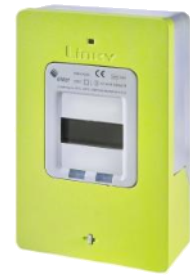
\includegraphics[width=.4\columnwidth]{Pictures/linky.png}}
\end{wrapfigure}

Par exemple, le compteur électrique \Index{Linky} que tous les Français connaissent en implémente qu'une partie. Au lieu d'utiliser \ac{CoAP}, les électriciens utilisent leurs propres applications suivant la norme \ac{DLMS}/\ac{Cosem}. Celle-ci repose sur \ac{UDP} puis \ac{IPv6} et \Index{6LoWPAN} et finalement sur une variante de \Index{IEEE 802.15.4} adaptée pour transporter l'information sur les câbles électriques.

%\chapter{LA REPRESENTATION DE LA DONNEE}

\section{Introduction}
     \vspace{1em}

Envoyer une donnée sur un réseau n’est pas aussi simple que l’on croit.
     \vspace{1em}

Il faut faire la différence entre le format utilisé pour stocker des données dans la mémoire de l'ordinateur et celui employé pour l'envoyer à une autre machine. En effet, chaque machine à sa propre représentation souvent liée aux capacités de leur processeur. Cela est surtout vrai pour les nombres. Ils peuvent être stockés sur un nombre de bits plus ou moins important ou peuvent être représentés en mémoire de manière optimisée pour accélérer leur traitement. 

En revanche, la représentation des chaînes de caractères (non accentués) est relativement uniforme car elle se base sur le code ASCII qui est le même pour tous les ordinateurs. Un texte de base est facilement compréhensible par toutes les machines. Une solution serait donc de n'utiliser que des chaînes de caractères. 

     \vspace{1em}

Par exemple, si l’on veut envoyer l'entier ayant pour valeur 123, il existe plusieurs représentations possibles :
\begin{itemize}
\item envoyer une chaîne de caractères ”123” contenant les chiffres du nombre ;
\item envoyer la valeur binaire 1111011.
\end{itemize}

     \vspace{1em}

On voit que juste pour transmettre une simple valeur stockée dans la mémoire d'un ordinateur, il existe plusieurs options et évidemment pour que cette valeur soit interprétée de la bonne façon, il faut que les deux extrémités se soient mises d'accord sur une représentation.

Quand on veut transmettre plusieurs valeurs, c'est-à-dire quand on a des données structurées, d'autres problèmes surviennent.

Par exemple : quelle est la taille des blocs que l’on va transmettre ? Comment indiquer la fin de la transmission ? Pour une chaîne de caractères, comment indiquer qu’elle se termine ? Autre exemple : si l'on veut transmettre "12" puis "3", comment faire pour que l'autre extrémité ne comprenne pas "123" ?

     \vspace{1em}


Pour que la transmission se fasse correctement, il faut que l’émetteur et le récepteur adoptent les mêmes conventions. Quand il s’agit d’un ensemble de données, il faut être capable de les séparer. Avec les tableurs, une première méthode est possible avec la notation \ac{CSV} Comme son nom l’indique, les valeurs sont séparées par des virgules. Les valeurs sont représentées par des chaînes de caractères. Les textes sont différenciés des valeurs numériques, par l’utilisation de guillemets. Ainsi, 123 sera interprété comme un nombre et ”123” comme un texte.

Si cette représentation est adaptée aux tableurs, elle est relativement pauvre car elle ne permet de représenter que des valeurs sur des lignes et des colonnes. Pour les usages du Web, il a fallu trouver un format plus souple permettant de représenter des structures de données complexes. Évidemment, comme rien n'est simple, il en existe plusieurs et les applications échangeant des données devront utiliser le même.

     \vspace{1em}


On voit que l'envoi de la chaîne de caractères ne suffit pas, il faut la formater pour que le récepteur puisse trouver le type de la donnée transmise, qu'un nombre ne soit pas interprété comme une chaîne de caractères, qu'une chaîne de caractères reste une chaîne de caractères même si elle ne contient que des chiffres.   
    \vspace{1em}
   
\section{La \Index{sérialisation}}

Sous ce nom barbare se cache la méthode utilisée pour transmettre 
des données d’un ordinateur à un autre.
Une donnée peut être simple
(un nombre, un texte) ou plus complexe (un tableau, une structure...). 
Elle est stockée dans la mémoire de l'ordinateur suivant une représentation qui lui est propre. Par exemple, la taille des entiers peut varier d'une technologie de processeur à une autre, l'ordre des octets dans un nombre peut aussi être différente (little et big endian). 
Pour des structures complexes comme les tableaux, les éléments peuvent être rangés à différents emplacements de la mémoire. 

La sérialisation consiste à transformer une structure de données en une séquence qui pourra être transmise sur le réseau, stockée dans un fichier ou une base de données. L'opération inverse, consistant à reconstruire localement une structure de données, s'appelle désérialisation. 

Il existe plusieurs formats pour sérialiser les données. Ils peuvent être binaires mais ceux généralement utilisés sont basés sur des chaînes de caractères. En effet, la représentation \ac{ASCII} définissant les caractères de base et codée sur 7 bits est commune à l'ensemble des ordinateurs. L'autre avantage du code ASCII est qu'il est facilement lisible et simplifie la mise au point des programmes.  

Wikipédia donne ce tableau (cf. figure~\vref{fig-ASCII}) des codes \ac{ASCII} datant de 1972 (une éternité en informatique) et recolorisé par nos soins.

\begin{figure}[tbp]
\centerline{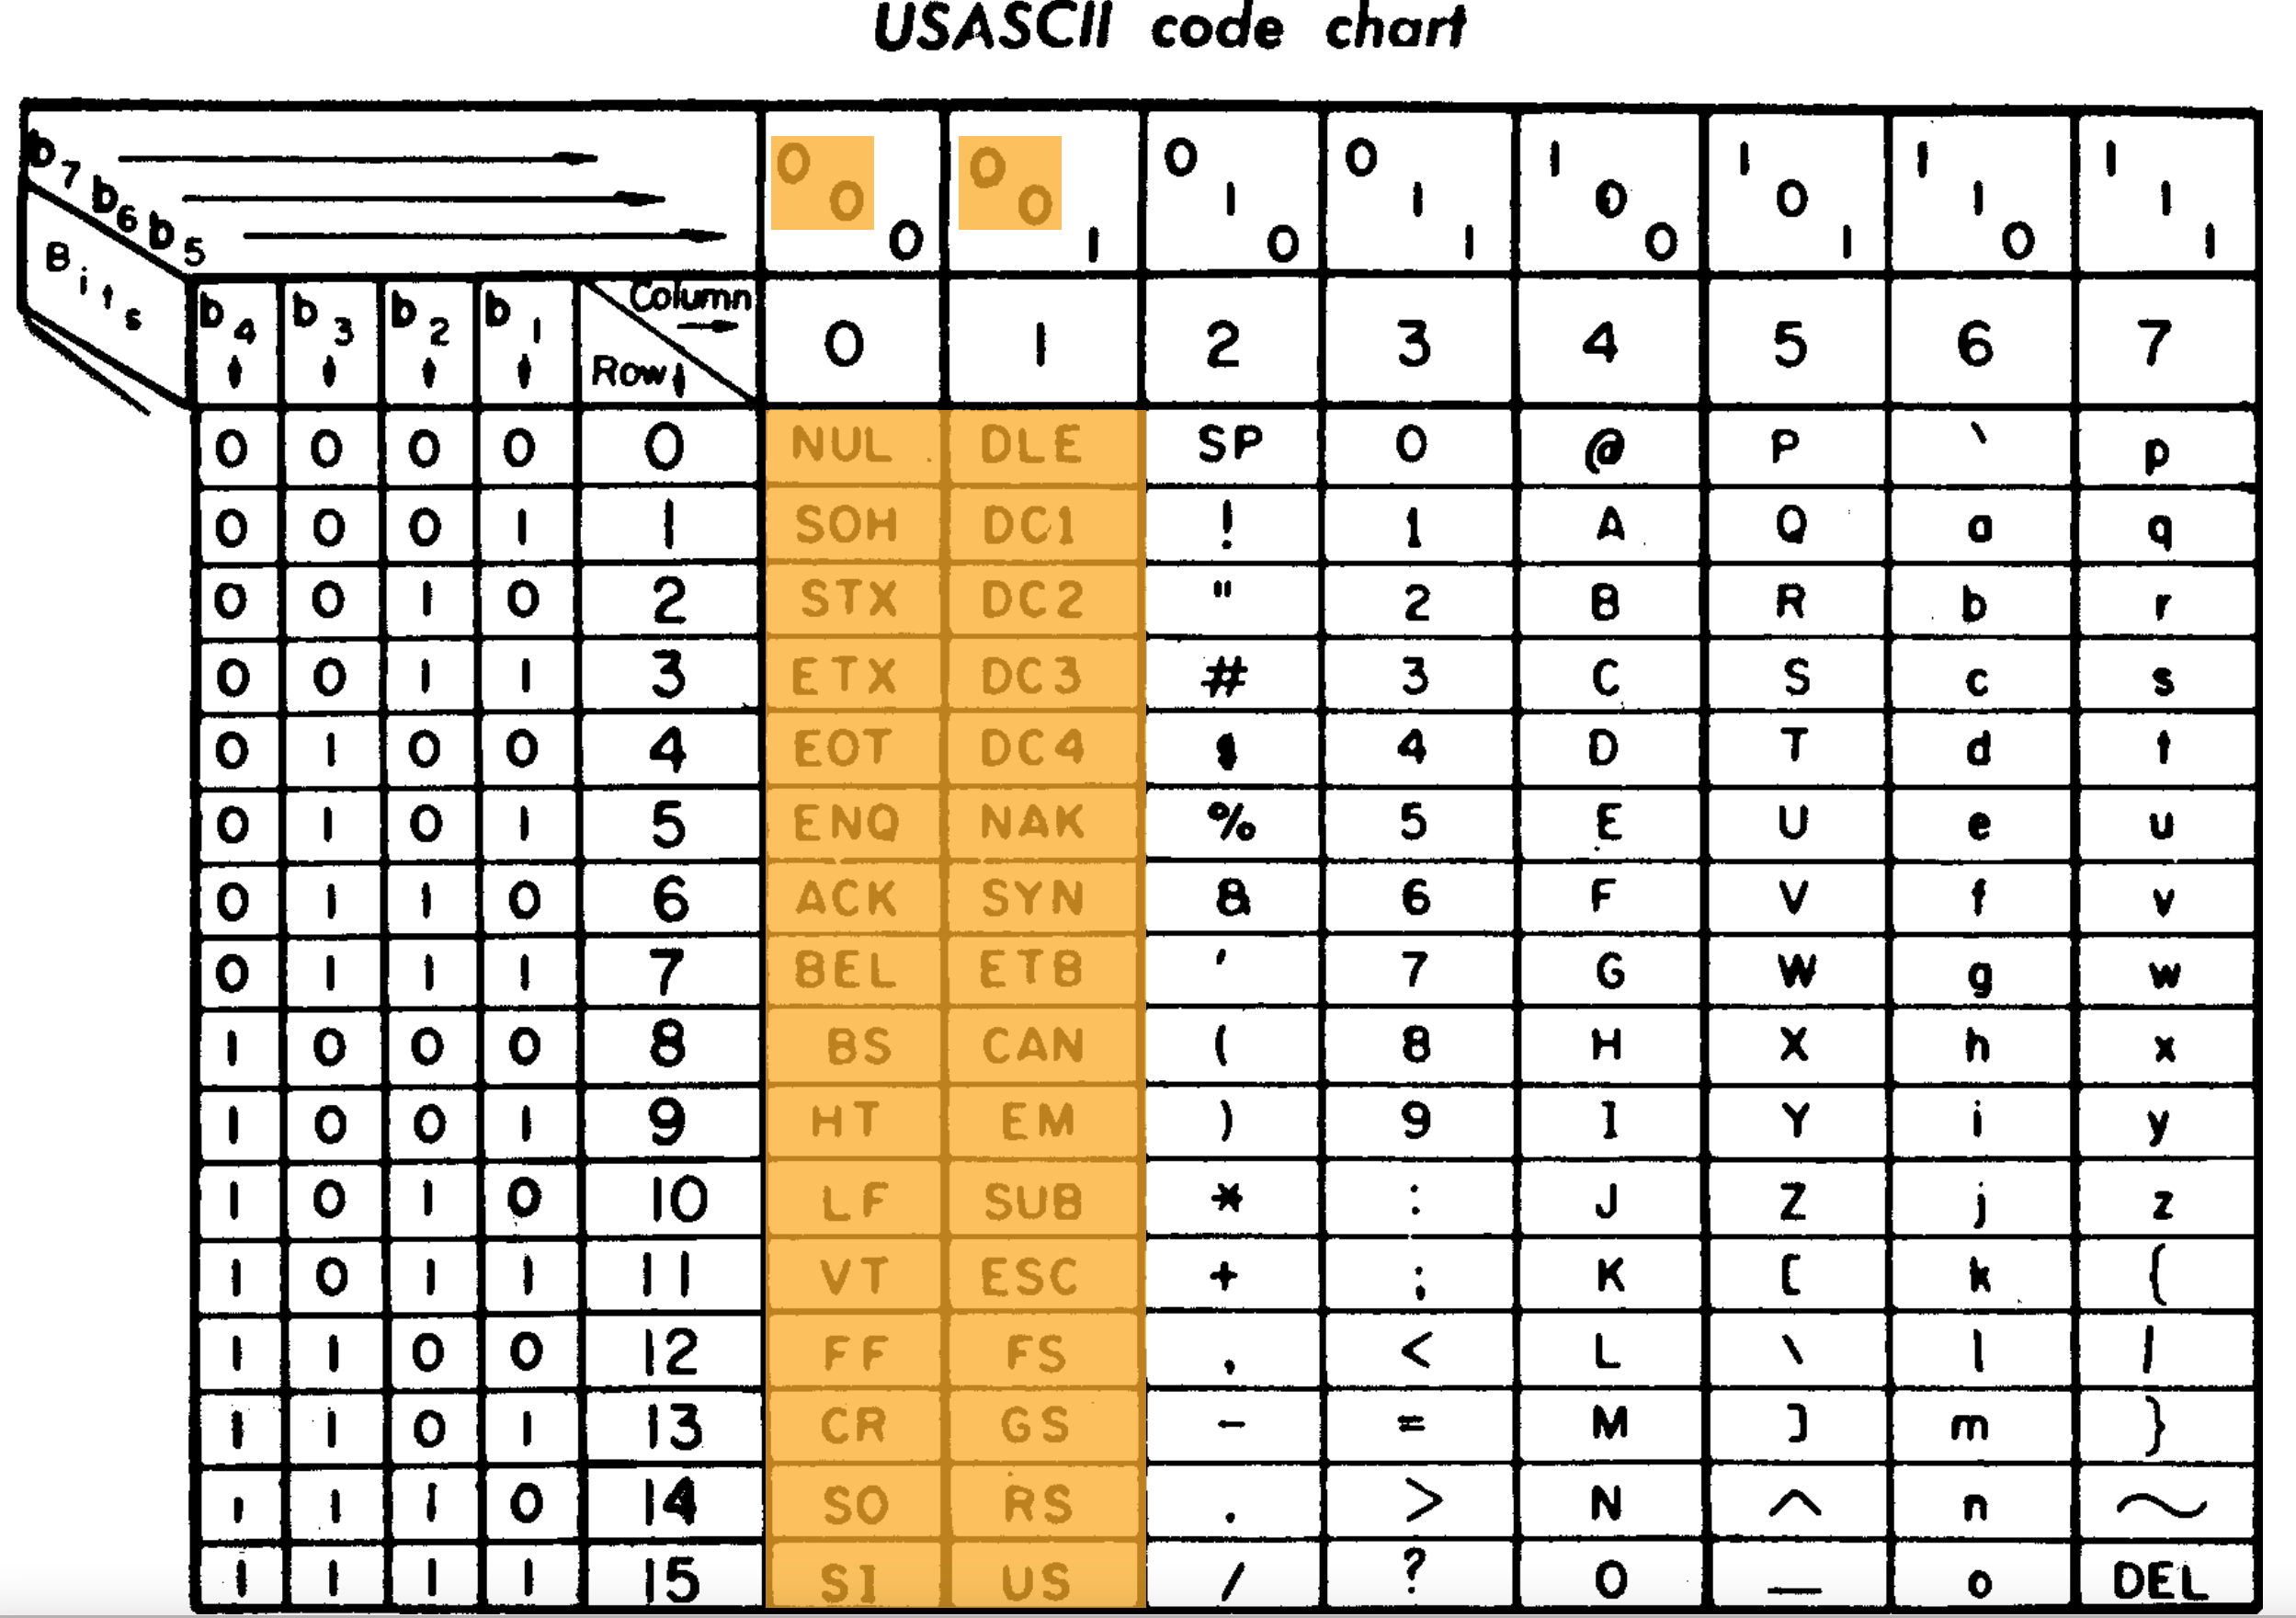
\includegraphics[width=1\columnwidth]{Pictures/Capture20.png}}
\caption{Codage ASCII des caractères}
\label{fig-ASCII}
\end{figure}

Les caractères en orange ne sont pas imprimables. Ils permettent de contrôler la communication des données ou de gérer l'affichage en revenant à la ligne. On les reconnait car la séquence binaire commence par 00X XXXX. On rappelle que le code ASCII est sur 7 bits ; le bit supplémentaire (bit de parité) conduisant à 1 octet était utilisé pour détecter des erreurs de transmission. Les valeurs de 0x30 à 0x39 codent les chiffres de 0 à 9. 

\subsection*{Hexlify}

En Python, il existe le module \Index{binascii} très pratique qui permet de convertir une séquence binaire en une chaîne de caractères ou inversement :
\begin{itemize}
\item \pfunction{binascii}{hexlify} prend un tableau d'octets et le convertit en une chaîne de caractères hexadécimaux plus lisible pour les spécialistes. Cela permet de visualiser n'importe quelle séquence de données. 
\item \pfunction{binascii}{unhexify} fait l'inverse. Il prend une chaîne de caractères et la convertit en un tableau d'octets. Cela peut vous faciliter la programmation car, dans votre code, il est plus facile de manipuler des chaînes de caractères.

\end{itemize}
Dans la suite, nous l'utiliserons pour manipuler des identifiants. Par exemple, ce bout de code illustre l'utilisation de ces fonctions :

\begin{python}
mac = lora.mac()
print ('devEUI: ',  binascii.hexlify(mac))

# create an OTAA authentication parameters
app_eui = binascii.unhexlify('70 B3 D5 7E D0 03 3A E3'.replace(' ',''))

\end{python}

Comme nous le verrons par la suite, a fonction \pfunction{network}{lora.mac()} retourne un tableau d'octets. La fonction \pfunction{binascii}{hexlify} ligne suivante le convertit en chaîne de caractères pour un affichage plus propre. 

Inversement, nous devons affecter une séquence binaire à la variable \texttt{app\_eui}. Nous mettons cette séquence hexadécimale en chaîne de caractères. Les espaces offrent plus de lisibilité. Ils sont retirés par la méthode replace et le résultat est converti en binaire grâce à \pfunction{binascii}{unhexify}

\section{Base64}

Le passage d'une séquence binaire à une chaîne de caractères ASCII en représentant les valeurs conduit à un doublement du volume. Chaque bloc de 4 bits va conduire à produire un octet correspondant au caractère d'un chiffre ou d'une lettre de A à F. Le reste des codes n'est pas utilisé.

Le codage base64 offre un meilleur rendement en utilisant 64 bits pour coder les valeurs. Un dictionnaire fait la correspondance entre 64 valeurs et un caractère ASCII. Cependant, si l'on veut coder 4 octets, soit 32 bits, il faudra 5 blocs de 6 bits, et il y aura deux bits restants. Le symbole = indique que 2 bits sont ajoutés à la fin du codage. Donc, dans notre cas, il faudra ajouter deux symboles = comme le montre la figure ci-dessous :

\begin{figure}[tbp]
\centerline{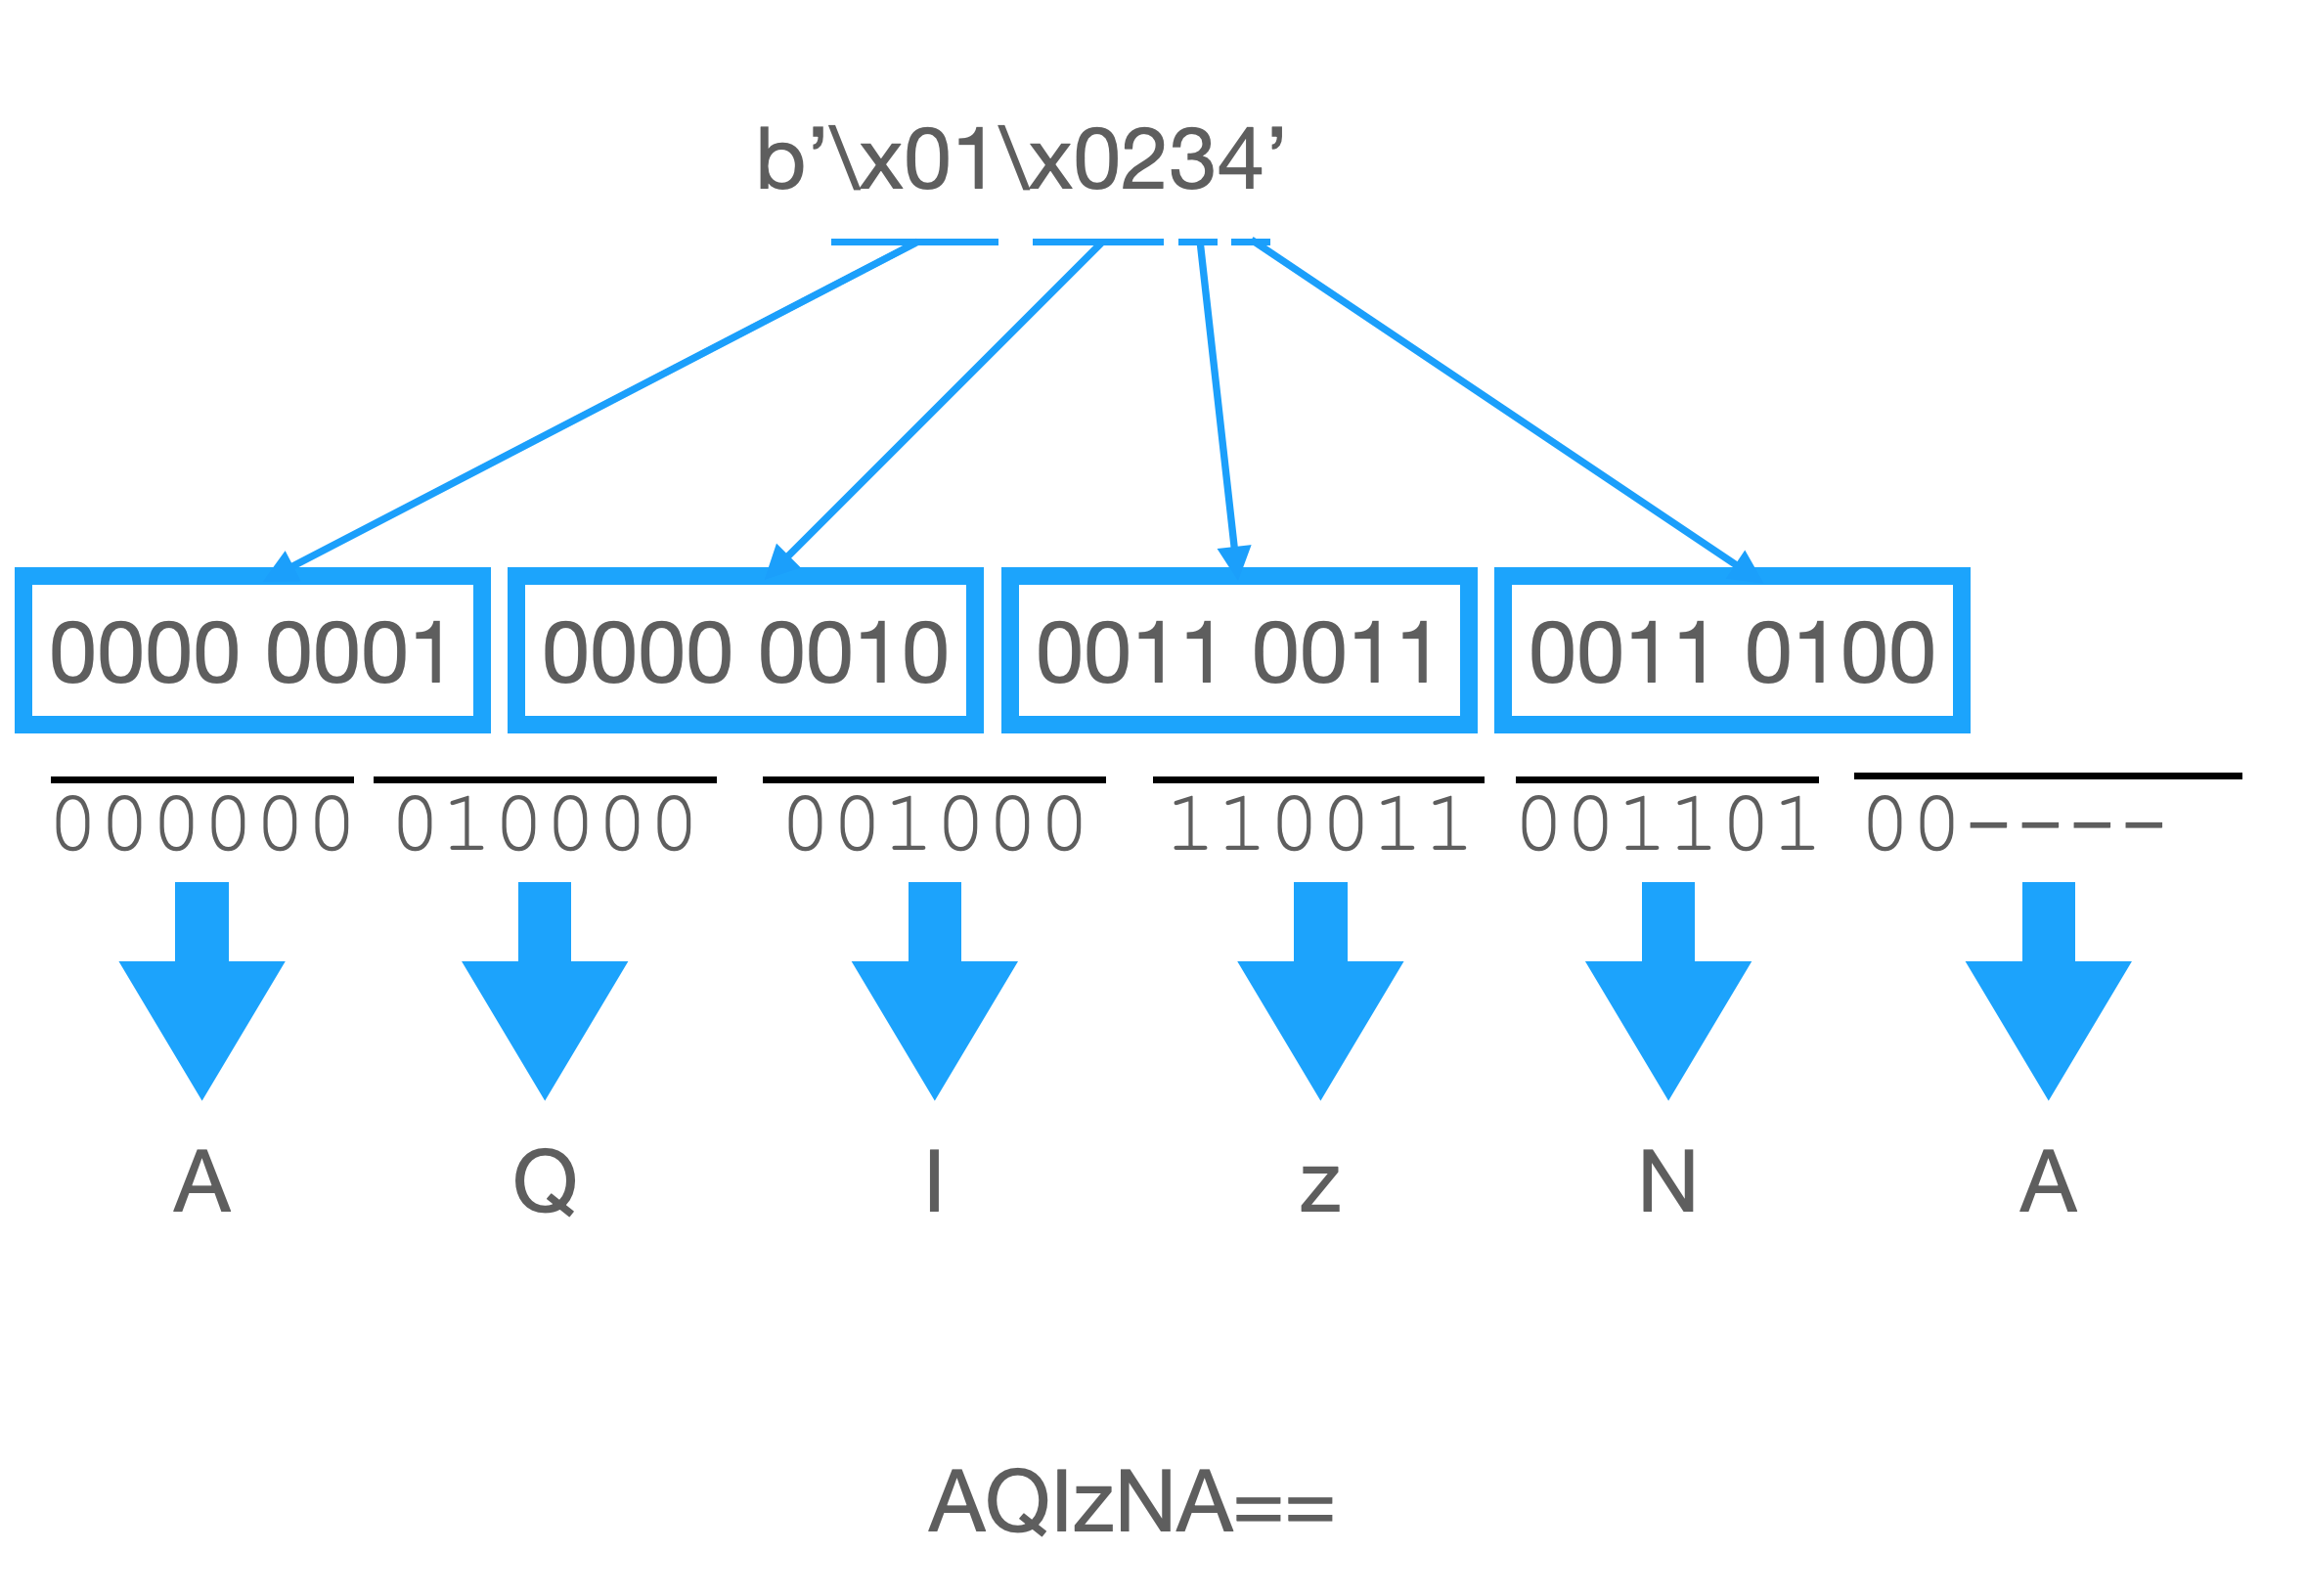
\includegraphics[width=1\columnwidth]{Pictures/Capture21.png}}
\caption{Codage Base64 de données binaires}
\label{fig-base64}
\end{figure}

On notera que pour les petites séquences, ce codage n'est pas meilleur que la transformation de la séquence hexadécimale en chaîne de caractères. Ici, il faut 8 caractères pour coder 4 octets. 

Il existe beaucoup d'outils en ligne pour faire les conversions entre ces différentes représentations, comme le site \url{www.asciitohex.com}.

\subsection*{Python module: base64}

En Python3, le module base64 permet de faire ces conversions.  Ce module est un peu susceptible sur les types de données à utiliser.

\begin{python}[numbers=left,numbersep=5pt]
import base64

val = b"\x01\x0234"
ser = base64.b64encode(val)
print (ser)
print (ser.decode())
ori = base64.b64decode(ser)
print (ori)
\end{python}

qui donne à l’exécution :

\begin{termc}[backgroundcolor=\color{backcolour}]
b'AQIzNA=='
AQIzNA==
b'\x01\x0234'
\end{termc}

À noter que l'utilisation du \texttt{ser.\pfunction{str}{decode()}}, ligne 6, pour transformer une chaîne d'octets en chaîne de caractères, c'est-à-dire supprimer le \texttt{b} du début, peut être utilisé dans certains cas.



\section{HTML}

La sérialisation en chaînes de caractères (par exemple en Python via la commande \pfunction{binascii}{hexlify}) ou en Base64 concerne surtout des données binaires. Mais la donnée peut être aussi structurée, par exemple la page d'un tableur. Il faut donc formater le document pour éviter une fusion des différents champs.


\ac{HTML}, sans entrer dans les détails, définit un format où les champs sont repérés par un balisage.  Une balise de début est un mot clé entre \texttt{<>} et, pour une \Index{balise} de fin, le mot clé est précédé du caractère \texttt{/}. Par exemple, la figure~\vref{fig-HTML} avec le balisage, le premier paragraphe est formaté de cette manière, Dans le MOOC :

\begin{figure}[tbp]
\centerline{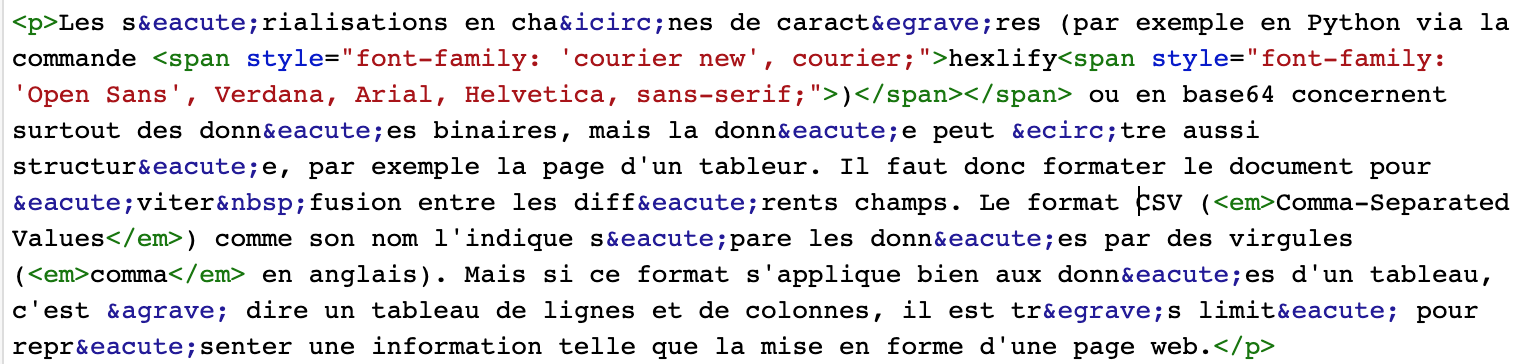
\includegraphics[width=1\columnwidth]{Pictures/Capture22.png}}
\caption{Codage HTML d'une page Web}
\label{fig-HTML}
\end{figure}

Les balises peuvent aussi prendre des arguments, comme la balise \Index{span} dans l'exemple précédent. Ainsi, si l'on regarde une page Web, comme indiqué figure~\vref{fig-Web-HTML}, le navigateur est capable de l'analyser pour trouver les \ac{URI} qu'elle contient. La balise \texttt{\Index{img}} indiquant qu'il s'agit d'une image, le client peut interroger le serveur pour l'afficher à l'écran. Ce format structuré de sérialisation nous permet de mettre en place une caractéristique de \ac{REST}, c'est-à-dire les liens entre ressources.

\begin{figure}[tbp]
\centerline{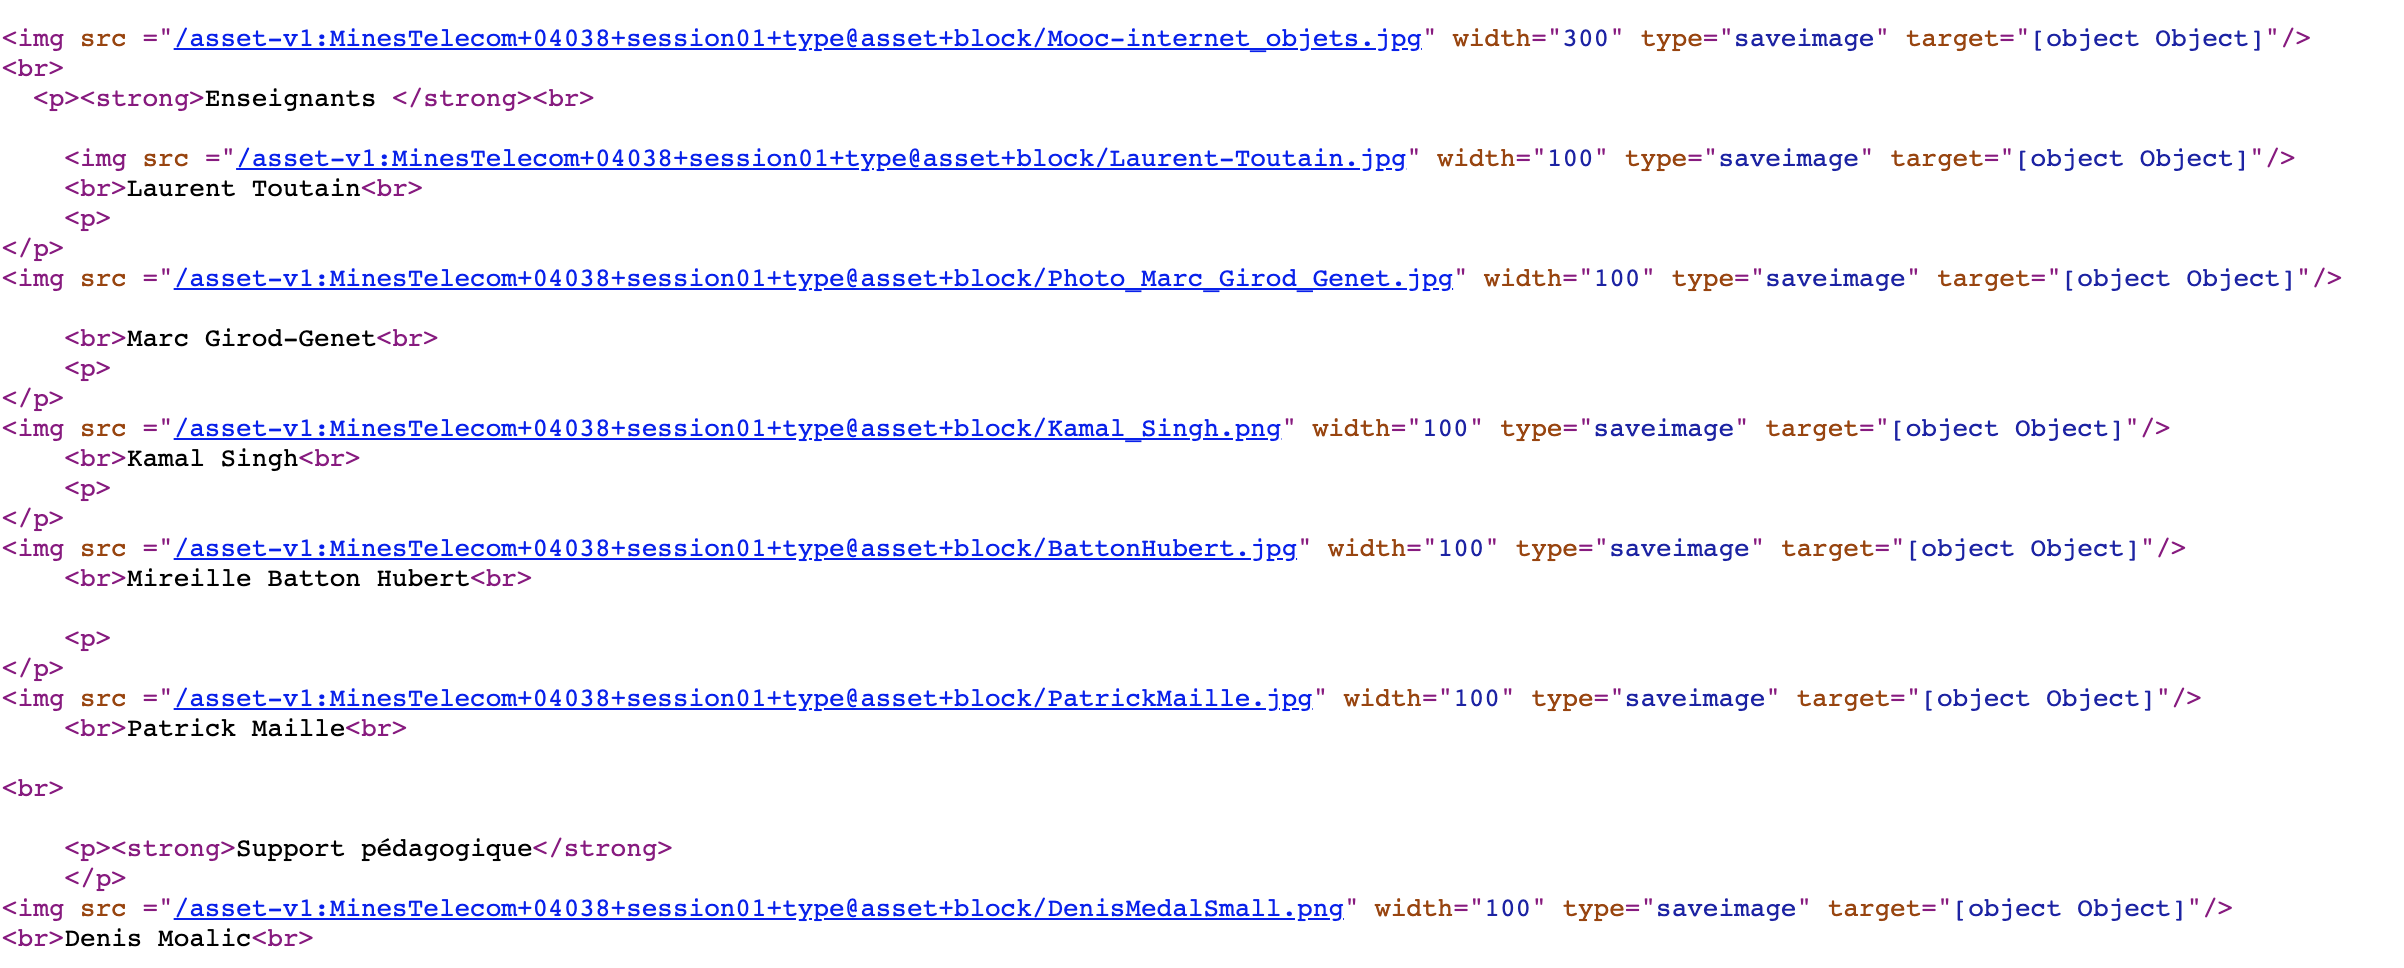
\includegraphics[width=1\columnwidth]{Pictures/Capture23.png}}
\caption{Capture d'une page Web}
\label{fig-Web-HTML}
\end{figure}


\section{XML}

Si \ac{HTML} est dédié au formatage à l'écran de données textuelles et à la navigation sur le Web. \ac{XML}\footnote{\url{https://www.w3.org/TR/xml/}} défini par le \ac{W3C}, est un format d’échange entre deux applications. Par exemple, pour échanger les notes des étudiants entre la plate-forme FUN et une autorité de certification des cours, on pourrait utiliser le format suivant~:

\begin{termc}[backgroundcolor=\color{gray!10}]
<etudiant>
   <prenom>John</prenom>
   <nom>Deuf</nom>
   <note>18</note>
</etudiant>

\end{termc}

Il est facile en lisant l'exemple de trouver le prénom, le nom et la note de l'étudiant. On peut noter qu'il n'y a pas de différence entre la note et le nom de l'élève. Il s'agit de caractères.

     \vspace{1em}

S'il est syntaxiquement correct, rien ne dit que le créateur fournit quelque chose de correct qui pourra être interprété par une autre instance.  \ac{XML} peut inclure une grammaire ou un schéma qui est utilisé pour valider que les informations représentées dans le fichier sont non seulement syntaxiquement conformes au langage \ac{XML}, mais aussi conformes au schéma. Ce schéma va décrire les champs attendus et leur type (texte, nombre...). Vous pouvez accéder à ce cours si vous voulez en savoir plus sur les schémas \ac{XML}.

Du point de vue de l’internet des objets, même si le XML pourrait être un bon candidat pour l’échange d’informations, il est un format trop lourd et donc énergivore. On peut noter que pour envoyer une note sur 20 qui, dans l'absolu, prendrait 6 bits, on transmet \texttt{<note>18</note>}, soit 15 caractères soit 120 bits! 

\section{JSON}

\ac{JSON}  offre un moyen de structurer l’information de manière plus compacte que \ac{XML}. JSON s’impose comme le langage commun pour échanger les informations. A l’origine, JSON était utilisé par\Index{Javascriptt} pour échanger des informations ; par exemple, pour afficher en temps réel l’évolution des cours de la bourse ou pour afficher des graphiques dynamiques sur l’écran de l’utilisateur.

JSON \rfc{8259} est un format d’échange simple. Il définit 4 types de données :

\begin{itemize}
    \item nombre~: Les nombres sont composés de chiffres et peuvent être positifs, négatifs, entiers ou flottants.
    \item texte~: Le texte est délimité par des guillemets simples ou doubles.
    \item \Index{tableau}~: Les tableaux sont des listes d’éléments séparés par des virgules et entourés de crochets.
    \item \Index{objet}~: L’objet est une liste de paires composées d’une \Index{clé} et d’une valeur. La clé est une chaîne de caractères et la valeur peut être de n’importe quel type. La clé doit être unique à l’intérieur d’un objet, et référence entièrement la valeur qui la suit. Le couple clé - valeur est séparé par le caractère 2 points  \texttt{:}. Les éléments de l’objet sont séparés par des virgules. L'objet est délimité par des accolades.
\end{itemize}

Par exemple, quelques structures \ac{JSON} :

\begin{itemize}
    \item \texttt{[1, -2, 0.3, 4e1]} est un tableau qui contient 4 nombres ;
    \item \texttt{[1, ”2”, ”34”]} est un tableau contenant un nombre et deux chaines de caractères ;
    \item \texttt{[1, [2, 3 , ”4”]]} est un tableau de deux éléments dont le second est également un tableau de 3 éléments ;
    \item \texttt{\{ ”couleur” : [34, 16, 3]\}} est un objet qui contient un élément et la valeur est un tableau ; 
    \item \texttt{\{ ”name” : ”bob”, ”age” : 30\}} est un objet qui contient deux éléments référencés par les chaînes de caractères (ou index)  ”name” et ”age”.
    
    L’ordre dans lequel sont placés les éléments est indifférent. \texttt{\{”age” : 30, ”name” : ”bob”\}} est équivalent au dernier exemple. 

    Cela impose que l’index utilisé pour accéder à une valeur doit être unique dans la structure objet \texttt{\{”name” : ”bob”, ”name” : ”alice”}\} est interdit.
\end{itemize}

     \vspace{1em}

Le listing suivant donne un exemple de structure JSON tirée du \rfc{8259}. Il contient un objet JSON avec une seule clé \texttt{”Image”}. La valeur de cette clé est une autre structure qui contient six éléments. 

\begin{termc}[backgroundcolor=\color{gray!10}, language=json]
{
"Image": {
      "Width": 800,
      "Height": 600,
      "Title": "View from 15th Floor",
      "Thumbnail": {   
           "Url": "http://www.example.com/image/481989943",
           "Height": 125,
           "Width": 100
       },
       "Animated" : false,
       "IDs": [11, 943, 234, 38793]
    }
}
\end{termc}

Le balisage par clé est un élément fondamental dans la structure des données. Il est primordial d'être cohérent et d'assurer une concordance entre émetteur et récepteur sur l'intitulé de la clé pour pouvoir récupérer l'information voulue. De la même façon, il faut s'accorder sur les unités de mesure : une interprétation d'une mesure en centimètre alors qu'elle est en pixel peut être désastreux ; c'est un problème d'interopérabilité.
     \vspace{1em}

JSON est facilement exploitable dans d’autres langages. Par exemple en Python, le module JSON peut être utilisé pour convertir une structure JSON qui est une chaîne ASCII en une représentation interne Python. Les tableaux sont convertis en listes et les objets en dictionnaires.

     \vspace{1em}
     \pythonlst{example\_json.py}

Le programme \pprog{example\_json.py} reprend la structure précédente. La variable \texttt{struct\_python} est une structure Python. On peut voir que les valeurs pour \texttt{"Animated"} et \texttt{"Copyright"} sont les mots clé Python \texttt{False} (avec un F majuscule) et \texttt{None}. Le programme affiche deux fois cette valeur avec la commande standard \texttt{print} puis avec le module \pfunction{pprint}{pprint} pour avoir un affichage plus lisible. On peut remarquer que l'ordre d'affichage des clés est différent. Comme \texttt{"Title"} était défini deux fois, seul le dernier est conservé dans la structure Python.

\begin{termc}[backgroundcolor=\color{gray!10}, language=json, basicstyle=\tiny]
{'Image': {'IDs': [17, 2371, 234, 38793], 'Height': 600, 'Animated': False, 'Title': 'Empty picture', 'Thumbnail': 
{'Url': 'http://www.example.com/image/481989943', 'Width': 100, 'Height': 125}, 'Width': 800, 'Copyright': None}}
{'Image': {'Animated': False,
           'Copyright': None,
           'Height': 600,
           'IDs': [17, 2371, 234, 38793],
           'Thumbnail': {'Height': 125,
                         'Url': 'http://www.example.com/image/481989943',
                         'Width': 100},
           'Title': 'Empty picture',
           'Width': 800}}
\end{termc}

Grâce à la fonction \pfunction{json}{dumps} du module \texttt{json}, la variable \texttt{struct\_python} est transformée en JSON. Les mots clé  \texttt{False} et  \texttt{None} sont remplacés par  \texttt{false} et  \texttt{null}. Le programme affiche une chaîne de caractères.

\begin{termc}[backgroundcolor=\color{gray!10}, language=json, basicstyle=\tiny]
{"Image": {"IDs": [17, 2371, 234, 38793], "Height": 600, "Animated": false, "Title": "Empty picture", "Thumbnail": 
{"Url": "http://www.example.com/image/481989943", "Width": 100, "Height": 125}, "Width": 800, "Copyright": null}}
\end{termc}

Pour le retransformer, de JSON en variable Python, on utilise la fonction inverse \pfunction{json}{loads} qui traduit une chaîne de caractères en variable Python.

\begin{termc}[backgroundcolor=\color{gray!10}, language=json, basicstyle=\tiny]
{'Image': {'Animated': False,
           'Copyright': None,
           'Height': 600,
           'IDs': [17, 2371, 234, 38793],
           'Thumbnail': {'Height': 125,
                         'Url': 'http://www.example.com/image/481989943',
                         'Width': 100},
           'Title': 'Empty picture',
           'Width': 800}}
\end{termc}


Les autres langues de programmation possèdent également leur propre bibliothèque pour effectuer la traduction.

     \vspace{1em}

Par rapport à \ac{XML}, \ac{JSON} est beaucoup plus permissif et manque de formalisme pour décrire la structure. \ac{JSON-LD} défini par le \ac{W3C} renforce l’interopérabilité de JSON en introduisant des clés spécifiques décrivant la structure des données, une référence aux unités, etc. Nous verrons ces concepts dans la suite du cours.


%\chapter{Mettre en œuvre un Capteur Virtuel}

\textit{Les programmes relatifs à cette section se trouvent dans le répertoire \texttt{plido-tp3}. Il est recommandé d'utiliser la machine virtuelle avec une fenêtre de terminal pour l'objet et une autre pour le serveur.}

\section {JSON}

\begin{wrapfigure}{r}{3cm}
\Youtube{https://youtu.be/mRuEiwa7Z74}
\end{wrapfigure}

Ca fait longtemps qu'on parle d'Internet des Objets, il est temps de mettre en pratique nos connaissances. On va commencer par une mise en oeuvre simple en Python sur votre machine. Le but dans cette partie est de tester tout ce qu'on a vu sans autre matériel qu'un ordinateur. Nous allons ouvrir deux fenêtres terminal. Dans l'une nous allons faire tourner un programme qui va émuler l'objet avec trois capteurs. Cet objet va communiquer avec un serveur qui va recueillir l'information. La communication se fera en interne avec une socket utilisant l'interface \Index{loopback} (cf. figure~\vref{fig-deux-terminaux}).


\begin{figure}[tbp]
\centerline{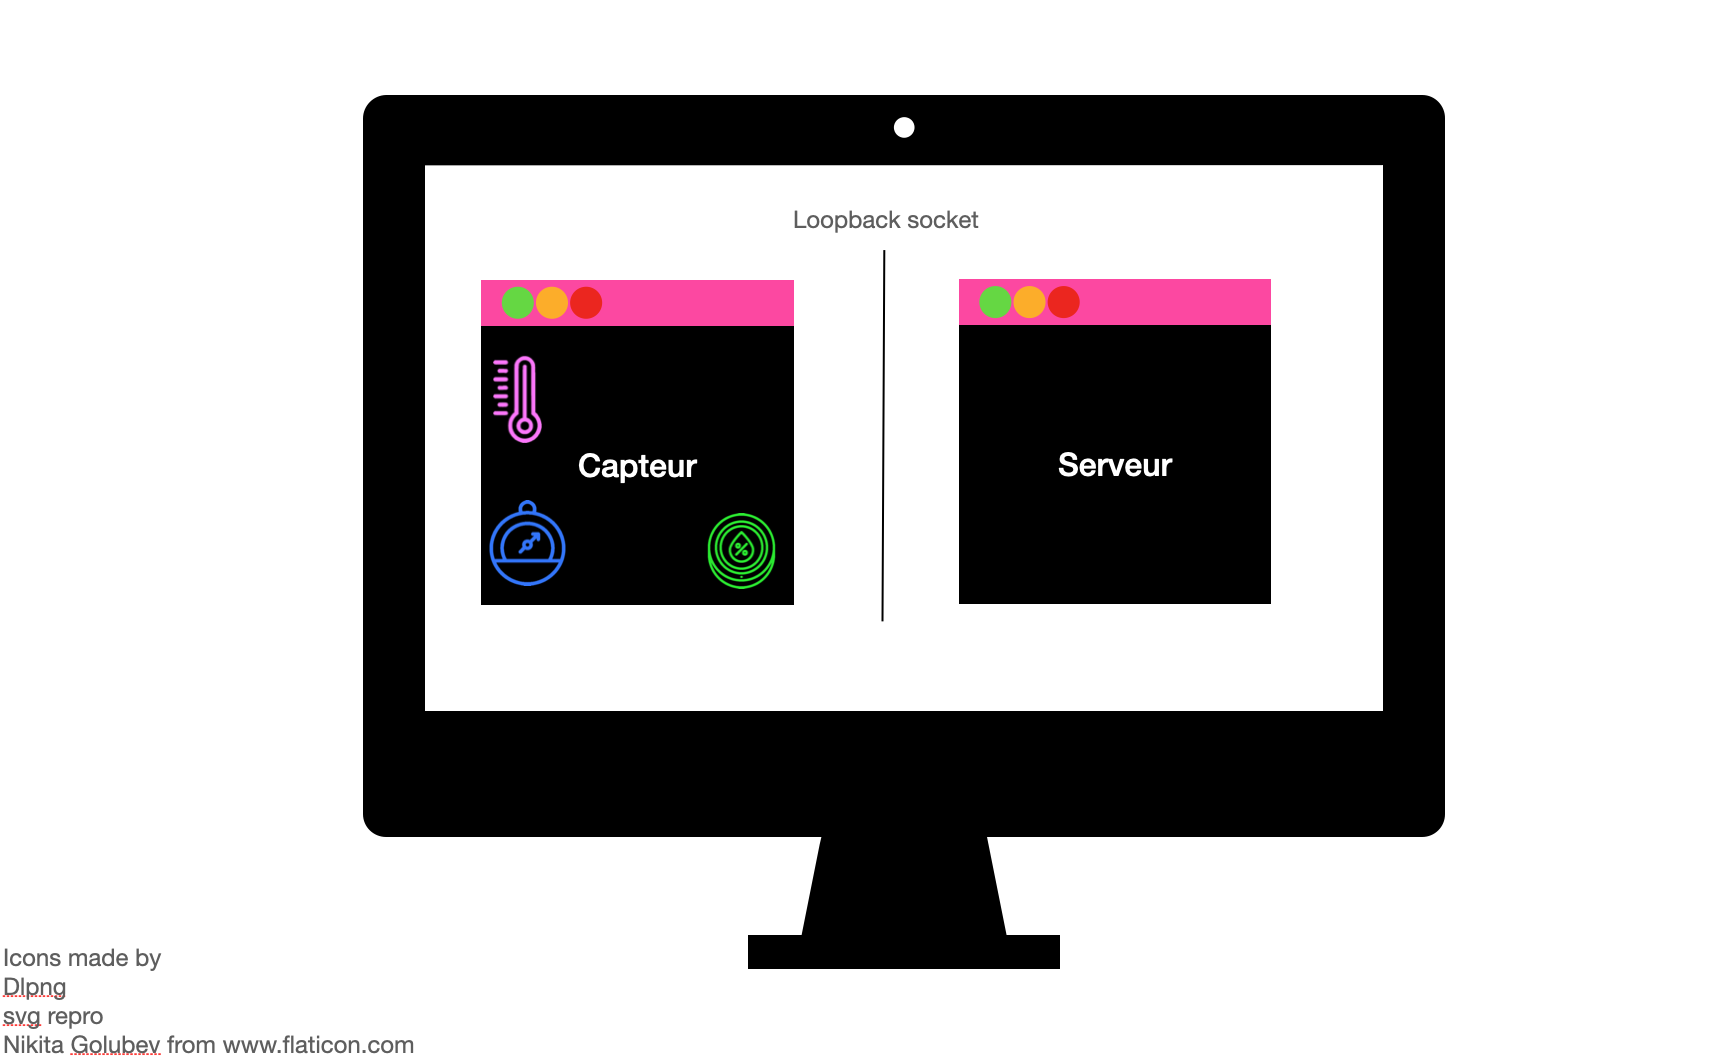
\includegraphics[width=1\columnwidth]{Pictures/Capture24.png}}
\caption{Architecture client serveur}
\label{fig-deux-terminaux}
\end{figure}

\subsection{Serveur Minimal}\label{chap-mini-serv}

\pythonlst{minimal\_server.py}


Commençons par construire un serveur sommaire (\texttt{minimal\_server.py}) qui va afficher tout ce qu'il reçoit. 
\begin{itemize}
    \item lignes 1 et 2 les modules \texttt{socket} pour la communication et \texttt{binascii} pour transformer le binaire en chaîne de caractères.
    \item ligne 4, la \pfunction{socket}{socket} crée la socket \texttt{s} avec les paramètres pour des communications IP (\texttt{AF\_INET}) et UDP (\texttt{SOCK\_DGRAM}).
    \item ligne 5, la socket est associée au numéro de port \texttt{33033} via la fonction \pfunction{socket}{bind}. L'adresse \texttt{0.0.0.0} indique que les données peuvent venir de n'importe quelle interface (Ethernet, Wi-Fi, loopback,...) 
    \item ligne 8, dans la boucle sans fin, la fonction \pfunction{socket}{recvfrom} va se bloquer dans l'attente de données. Elle retourne les données et l'adresse de l'émetteur.
    \item ligne 9, les données sont affichées en chaîne d'octets et en hexadécimal.
    
\end{itemize}

     \vspace{1em}

On lance le programme serveur. Comme personne lui parle, il n'affiche rien. 

\subsection{Capteur virtuel}

\pythonlst{virtual\_sensor.py}

Le module \Index{virtual\_sensor} avec la classe du même nom, reflète de manière à peu près réaliste le comportement d'un capteur. On voit dans le programme principal (ligne 23 à 37) que l'on créé trois capteurs virtuels : un pour la température (ligne 31), un autre pour la pression (ligne 32), et le troisième pour l'humidité (ligne 34). L'argument \texttt{start} précise la valeur de départ, \texttt{variation} la plage de variation entre deux mesures et \texttt{min} et \texttt{max} les valeurs à ne pas dépasser. La boucle sans fin qui affiche les différentes valeurs toutes les secondes.

\begin{termc}[backgroundcolor=\color{palerod}, language=json, basicstyle=\ttfamily\small, escapechar=@]
> @\textbf{python3 virtual\_sensor.py}@
 54.956    999.850  30.609
 54.963   1000.473  32.505
 55.062   1000.845  31.870
 55.017   1001.619  32.257
 55.083   1000.767  31.757
 55.027   1001.442  31.742
 \end{termc} 

\subsubsection{Envoi direct}

\pythonlst{minimal\_client1.py}
Des scripts utilisant ce module peuvent être écrit, comme par exemple le programme \texttt{minimal\_client1.py}.

La variable \texttt{t} contient la température qui est émise sur le port 33033 à l’adresse de \textit{loopback}. On obtient ainsi une communication entre deux programmes dans votre ordinateur dont l'adresse IP locale est \texttt{127.0.0.1}. Mais quand on lance le programme \texttt{minimal\_client1.py}, on obtient l’erreur suivante :

\begin{termc}[backgroundcolor=\color{palerod}, language=json, basicstyle=\ttfamily\small, escapechar=@]
 >python3.5 minimal_client1.py
Traceback (most recent call last):
  File "minimal_client1.py", line 11, in <module>
    s.sendto (t, ("127.0.0.1", 33033))
TypeError: a bytes-like object is required, not 'float'
\end{termc}

\Question{Bug ?}
{Pourquoi le programme client ne fonctionne pas ?
\begin{itemize}[label=$\circ$]
   \item \Wrong{L’adresse IP n’est pas correcte.}
   \item \Correct{Il manque un processus de sérialisation de la donné}
   \item \Wrong{La variable \texttt{t} n’est pas définie}
   \item \Wrong{La variable \texttt{t} ne peux pas être lue.}
 \end{itemize}
}
{La variable \texttt{t} pointe vers une représentation en mémoire du nombre flottant. Elle ne peut pas être directement envoyée à un autre équipement. Il faut ajouter une phase de sérialisation qui va permettre de transmettre cette information soit en une chaîne de caractères, soit en une chaîne d'octets.}

\subsubsection{Envoi d'une chaîne d'octets}

\pythonlst[firstline=9,lastline=11, firstnumber=9]{minimal\_client2.py}

Dans le programme \texttt{minimal\_client2.py}, le nombre flottant contenu dans la variable \texttt{t} est transformé en chaîne de caractères avec la fonction \texttt{\Index{str}}, puis en chaîne d'octets avec la méthode \pfunction{str}{encode} pour être compatible avec l'argument attendu par la méthode \pfunction{socket}{sendto}. Coté serveur la fonction \texttt{\Index{str}} converti la chaîne d'octets reçue en flottant.

\subsubsection{Envoi de plusieurs valeurs}

\pythonlst[firstline=11,lastline=17, firstnumber=11]{minimal\_client3.py} % 

Pour envoyer simultanément les valeurs des trois capteurs, la représentation via une chaîne de caractères est un peu plus compliquée à mettre en oeuvre. Si le programme \texttt{minimal\_client3.py} utilise \pfunction{str}{format} pour envoyer des données séparées par des vigules. Côté serveur, il faut décoder cette chaîne pour y retrouver les entiers. Et ça c'est beaucoup plus complexe à faire ! 

\subsubsection{JSON}

\pythonlst[firstline=12,lastline=19, firstnumber=12]{minimal\_client4.py} %

La solution la plus simple est de mettre ces trois valeurs dans un tableau python et de le transformer en une représentation JSON grâce à la fonction \pfunction{json}{dumps} du module \texttt{json}. 

     \vspace{1em}

Cette chaîne de caractères JSON est à son tour transformé en chaîne d'octets avec encode et envoyée au serveur. Dans notre cas, le serveur ne fait qu'afficher la chaîne de caractères mais vous pouvez utiliser la méthode \pfunction{json}{loads} du module \texttt{json} pour desérialiser et en faire une structure Python dans le serveur, sur laquelle il est maintenant facile d'effectuer des opérations comme, par exemple, un calcul de moyenne.

\begin{termc}[backgroundcolor=\color{palerod}, language=json, basicstyle=\ttfamily\tiny, escapechar=@]
% @\textbf{python3 minimal\_server.py}@
b'[19.93044784157464, 999.1552628155773, 35.723583473834566]' => b'5b31392e39333034343738343135373436342c203939392e313535c...
b'[19.940155545405723, 998.7581534530281, 35.820037116376184]' => b'5b31392e3934303135353534353430353732332c203939382e3735...
b'[20.003803212269627, 999.3517302791449, 34.33544522779677]' => b'5b32302e3030333830333231323236393632372c203939392e33353...
\end{termc}

\section{CBOR}

\begin{wrapfigure}{r}{3cm}
\Youtube{https://youtu.be/PmudahiRWFw}
\end{wrapfigure}

Le passage de JSON à CBOR est très simple. Il suffit de changer un module \texttt{cbor} à la place du module de \texttt{json}. Le programme \texttt{minimal\_client5.py}~:
\begin{itemize}
    \item ligne 1 fait appel au module cbor2 en le renommant cbor
    \item le reste du programme est identique au précédent, ce n'est que dans la la sérialisation, ligne 18, que la fonction \texttt{json.\pfunction{json}{dumps}} est remplacée par \texttt{cbor.\pfunction{cbor2}{dumps}}. Le format retourné étant une chaîne d'octets, il n'est plus nécessaire de faire appel à la méthode \texttt{encode}.
\end{itemize}


     \vspace{1em}


Le programme \pprog{minimal\_server.py} n'est pas modifié puisqu'il ne fait qu'afficher ce qu'il reçoit. 







\begin{termc}[backgroundcolor=\color{palerod}, language=json, basicstyle=\ttfamily\small, escapechar=#]
> #\texttbf{python3 minimal\_server.py}#
b'\x83... => b'83fb40341086f3e8b66bfb408f3b7791c8d61ffb403fac15ba06088e'
b'\x83... => b'83fb40341d4d28495268fb408f33d502185c3dfb403d95a2c4981444'
\end{termc}


\pythonlst{minimal\_client5.py}

On obtient le résultat suivant. La séquence CBOR fait 28 octets de long, l'équivalant JSON aurait fait 60 octets. Même si cela divise par deux la taille des données à transmettre, le résultat n'est pas compact. Cela tient à la représentation des nombres flottants en CBOR, car ici les flottant sont codés sur 8 octets.

\Question{Décodage}{
Analysons la séquence reçue: \texttt{83fb40341086f3e8b66bfb408f3b7791c8d61ffb403fac 15ba06088e}

À quoi correspond l’octet 0x83 qui commence la structure CBOR reçue ?
\begin{itemize}[label=$\circ$]
   \item \Wrong{au codage de l'entier positif 131 .}
   \item \Wrong{au codage de l'entier négatif 132 .}
   \item \Correct{à la définition d'un tableau de 3 éléments.́}
   \item \Wrong{à la définition d'un map CBOR de 3 éléments}
   \item \Wrong{à la définition d'un tableau de taille non définie.}
 \end{itemize}
 }
 {
 0x83 s'écrit en binaire \texttt{100-0 0111}. \texttt{100} est le type majeur pour un tableau. La valeur \texttt{00111} est inférieure à 24. Il s'agit donc du nombre d'éléments du tableau, donc un tableau de 3 éléments.
 }

\Question{Flottant}
{Dans cette chaîne, uel est le marqueur CBOR (en hexadécimal) qui indique que l’on a un nombre flottant ?}
{0xFB, si on l'écrit en binaire on obtient \texttt{111-1 1100}. Le majeur correspond à la catégorie des flottant et des valeurs spéciales.}

\Question{Taille du flottant}
{Quelle est la taille de ce flottant en octets ?}
{8 octets~; la partie mineur \texttt{1 1100} indique qu'il s'agit d'un flottant codé sur 8 octets}

\subsubsection{Utilisation de nombres entiers}

Pour réduire la taille des données transmises, nous allons utiliser des nombres entiers. Nous aurons besoin d’une précision au centième (deux chiffres après la virgule). Pour ce faire, il suffit, du coté du client, de prendre la partie entière du nombre multiplié par 100 et, du côté du serveur, de diviser la valeur reçue par 100. La modification du code est mineure.

\pythonlst[firstline=17,lastline=18, firstnumber=17]{minimal\_client6.py}


\begin{termc}[backgroundcolor=\color{palerod}, language=json, basicstyle=\ttfamily\tiny, escapechar=#]
> #\texttbf{python3 minimal\_server.py}#
b'\x83\x19\x07\xd7\x1a\x00\x01\x86O\x19\x0c\xa7' => b'831907d71a0001864f190ca7'
b'\x83\x19\x07\xd4\x1a\x00\x01\x86f\x19\x0cJ' => b'831907d41a00018666190c4a'
b'\x83\x19\x07\xd4\x1a\x00\x01\x86\x92\x19\rP' => b'831907d41a00018692190d50'
\end{termc}

La modification est mineure et tient en 12 octets, mais il y a une diminution au niveau de l'interopérabilité, car les deux entités doivent connaître la transformation de la valeur liée à la multiplication par 100.

\Question{Anticipons la taille}
{ Quelle est la taille minimale et maximale de la structure CBOR envoyée, en prenant en compte les valeurs possibles.
}
{
\begin{itemize}
    \item La température peut évoluer raisonnablement entre -30 et +50, soit -3000 et +5000 après la transformation en entier. La taille minimale, si on envoie 0, la taille sera d'un octet. La taille maximale tiennent sur 3 octets (1 pour le type/longueur et 2 pour les valeurs) 
    \item La pression évolue autour de 1000, soit 100~000 après la transformation en entier. La taille sera toujours de 5 octets (1 pour le type/longueur, 4 pour les valeurs)
    \item Le taux d'humidité évolue entre 0 et 100 , soit 0 et 10 000 après la transformation en entier. L a taille entre 1 octet et 3 octets
\end{itemize}

Si on ajoute le type/longueur 0x83 pour indiquer un tableau de trois éléments, on obtient une taille minimale de 1+1+5+1= 8 octets et une taille maximale de 1+3+5+3 = 12 octets.
}

\chapter{Séries temporelles}

\begin{wrapfigure}{r}{3cm}
\Youtube{https://youtu.be/xrdCY4iN40s}
\end{wrapfigure}

Les capteurs virtuels que nous avons programmés jusqu’à présent émettent les données à chaque fois que celles-ci sont mesurées. 
Cela permet au serveur de suivre en temps réel le comportement du système étudié. 
Mais dans certains cas, le temps réel n’est pas nécessaire et il est préférable de limiter le nombre d’émissions, par exemple pour économiser l'énergie du capteur.

Pour ce faire, nous pouvons utiliser un tableau qui va accumuler les valeurs et l’envoyer quand le tableau atteint une certaine taille.


\section{Envoi d'un tableau}

Le programme \pprog{minimal\_humidity1.py} accumule les données dans un tableau \texttt{h\_humidity} quand celui-ci atteint 30 éléments (ligne 17), les données sont envoyées au serveur.

\pythonlst{minimal\_humidity1.py}



\begin{termc}[backgroundcolor=\color{palerod}, basicstyle=\ttfamily\small, escapechar=\#]
1 4 [3241]
2 7 [3241, 2945]
3 10 [3241, 2945, 2762]
4 13 [3241, 2945, 2762, 2625]
5 16 [3241, 2945, 2762, 2625, 2480]
6 19 [3241, 2945, 2762, 2625, 2480, 2769]
\end{termc}

Le premier chiffre de la ligne indique le nombre d'éléments et le second la taille dans le codage CBOR. On remarque que l'ajout d'un élément augmente la taille du tableau de 3 octets. Les valeurs correspondant à une mesure d'humidité ne varient pas fortement. Ainsi un tableau de 30 mesures a une taille de 92 octets.

\section{Codage par différence}

On peut optimiser le volume de données transférées en utilisant un codage par delta (i.e. la variation de l'humidité). 
La première valeur du tableau correspond à la valeur mesurée tandis que les suivantes représentent la différence entre la valeur mesurée et la précédente.

\pythonlst[firstline=17,lastline=26,  firstnumber=17]{minimal\_humidity2.py}%[firstline=282,lastline=19, firstnumber=282]

Le programme \pprog{minimal\_humidity2.py} gère différemment le remplissage du tableau~:

\begin{itemize}
    \item ligne 14 et 15, si le tableau est vide, le tableau est créé avec la valeur mesurée,
    \item ligne 16 à 22, sinon si le tableau est plein, il est sérialisé en CBOR et envoyé au serveur, puis réinitialisé avec la valeur mesurée,
    \item ligne 23 et 24, sinon la différence entre la précédente valeur et celle mesurée est stockée dans le tableau.
\end{itemize}

       \vspace{1em}

Le listing suivant donne un exemple d'exécution.

\begin{termc}[backgroundcolor=\color{palerod}, basicstyle=\ttfamily\small, escapechar=\#]
1 4 [2521]
2 6 [2521, 79]
3 8 [2521, 79, 224]
4 10 [2521, 79, 224, -40]
5 12 [2521, 79, 224, -40, -112]
6 13 [2521, 79, 224, -40, -112, 1]
7 15 [2521, 79, 224, -40, -112, 1, 130]
8 18 [2521, 79, 224, -40, -112, 1, 130, -288]
9 21 [2521, 79, 224, -40, -112, 1, 130, -288, 299]
\end{termc}

Ceci met en valeur deux souplesses de CBOR :
\begin{itemize}
    \item la taille du tableau est dynamique. Si l’on change le nombre de valeurs à transmettre, le tableau l’indique et l’on n’a pas besoin de modifier le code du récepteur ;
    \item la taille des données dépend de leur valeur. 
    Pour les variations entre -24 et +23, un seul octet sera nécessaire. 
    On le voit sur l’exemple précédent : l’ajout de la valeur '1' dans le tableau fait passer la taille de la représentation CBOR de 12 à 135 octets. Les valeurs entre 256 et +255 sont transmises sur 2 octets ; il est donc possible de cette manière d’optimiser la transmission sans ajouter de contrainte. S’il y avait une brusque variation de l’humidité, la représentation CBOR s’adapterait pour la transmettre.
\end{itemize}

La taille est réduite d"un tiers (environ 66 octets) pour transmettre la même information.

\section{Architecture}

La figure~\vref{fig-client-serveur} représente l'architecture générale du système. Le programme \pprog{minimal\_humidity2.py} fournit les séries temporelles. Il reste à définir le programme serveur qui va les traiter et faire appel à un autre service pour les afficher sous forme de graphe. 

       \vspace{1em}


Si l'on suit le flux d'information, le capteur va produire des données au format CBOR pour être compact et le programme serveur va transformer cette information en une structure JSON respectant les spécifications du service d'affichage.

\begin{figure}[tbp]
\centerline{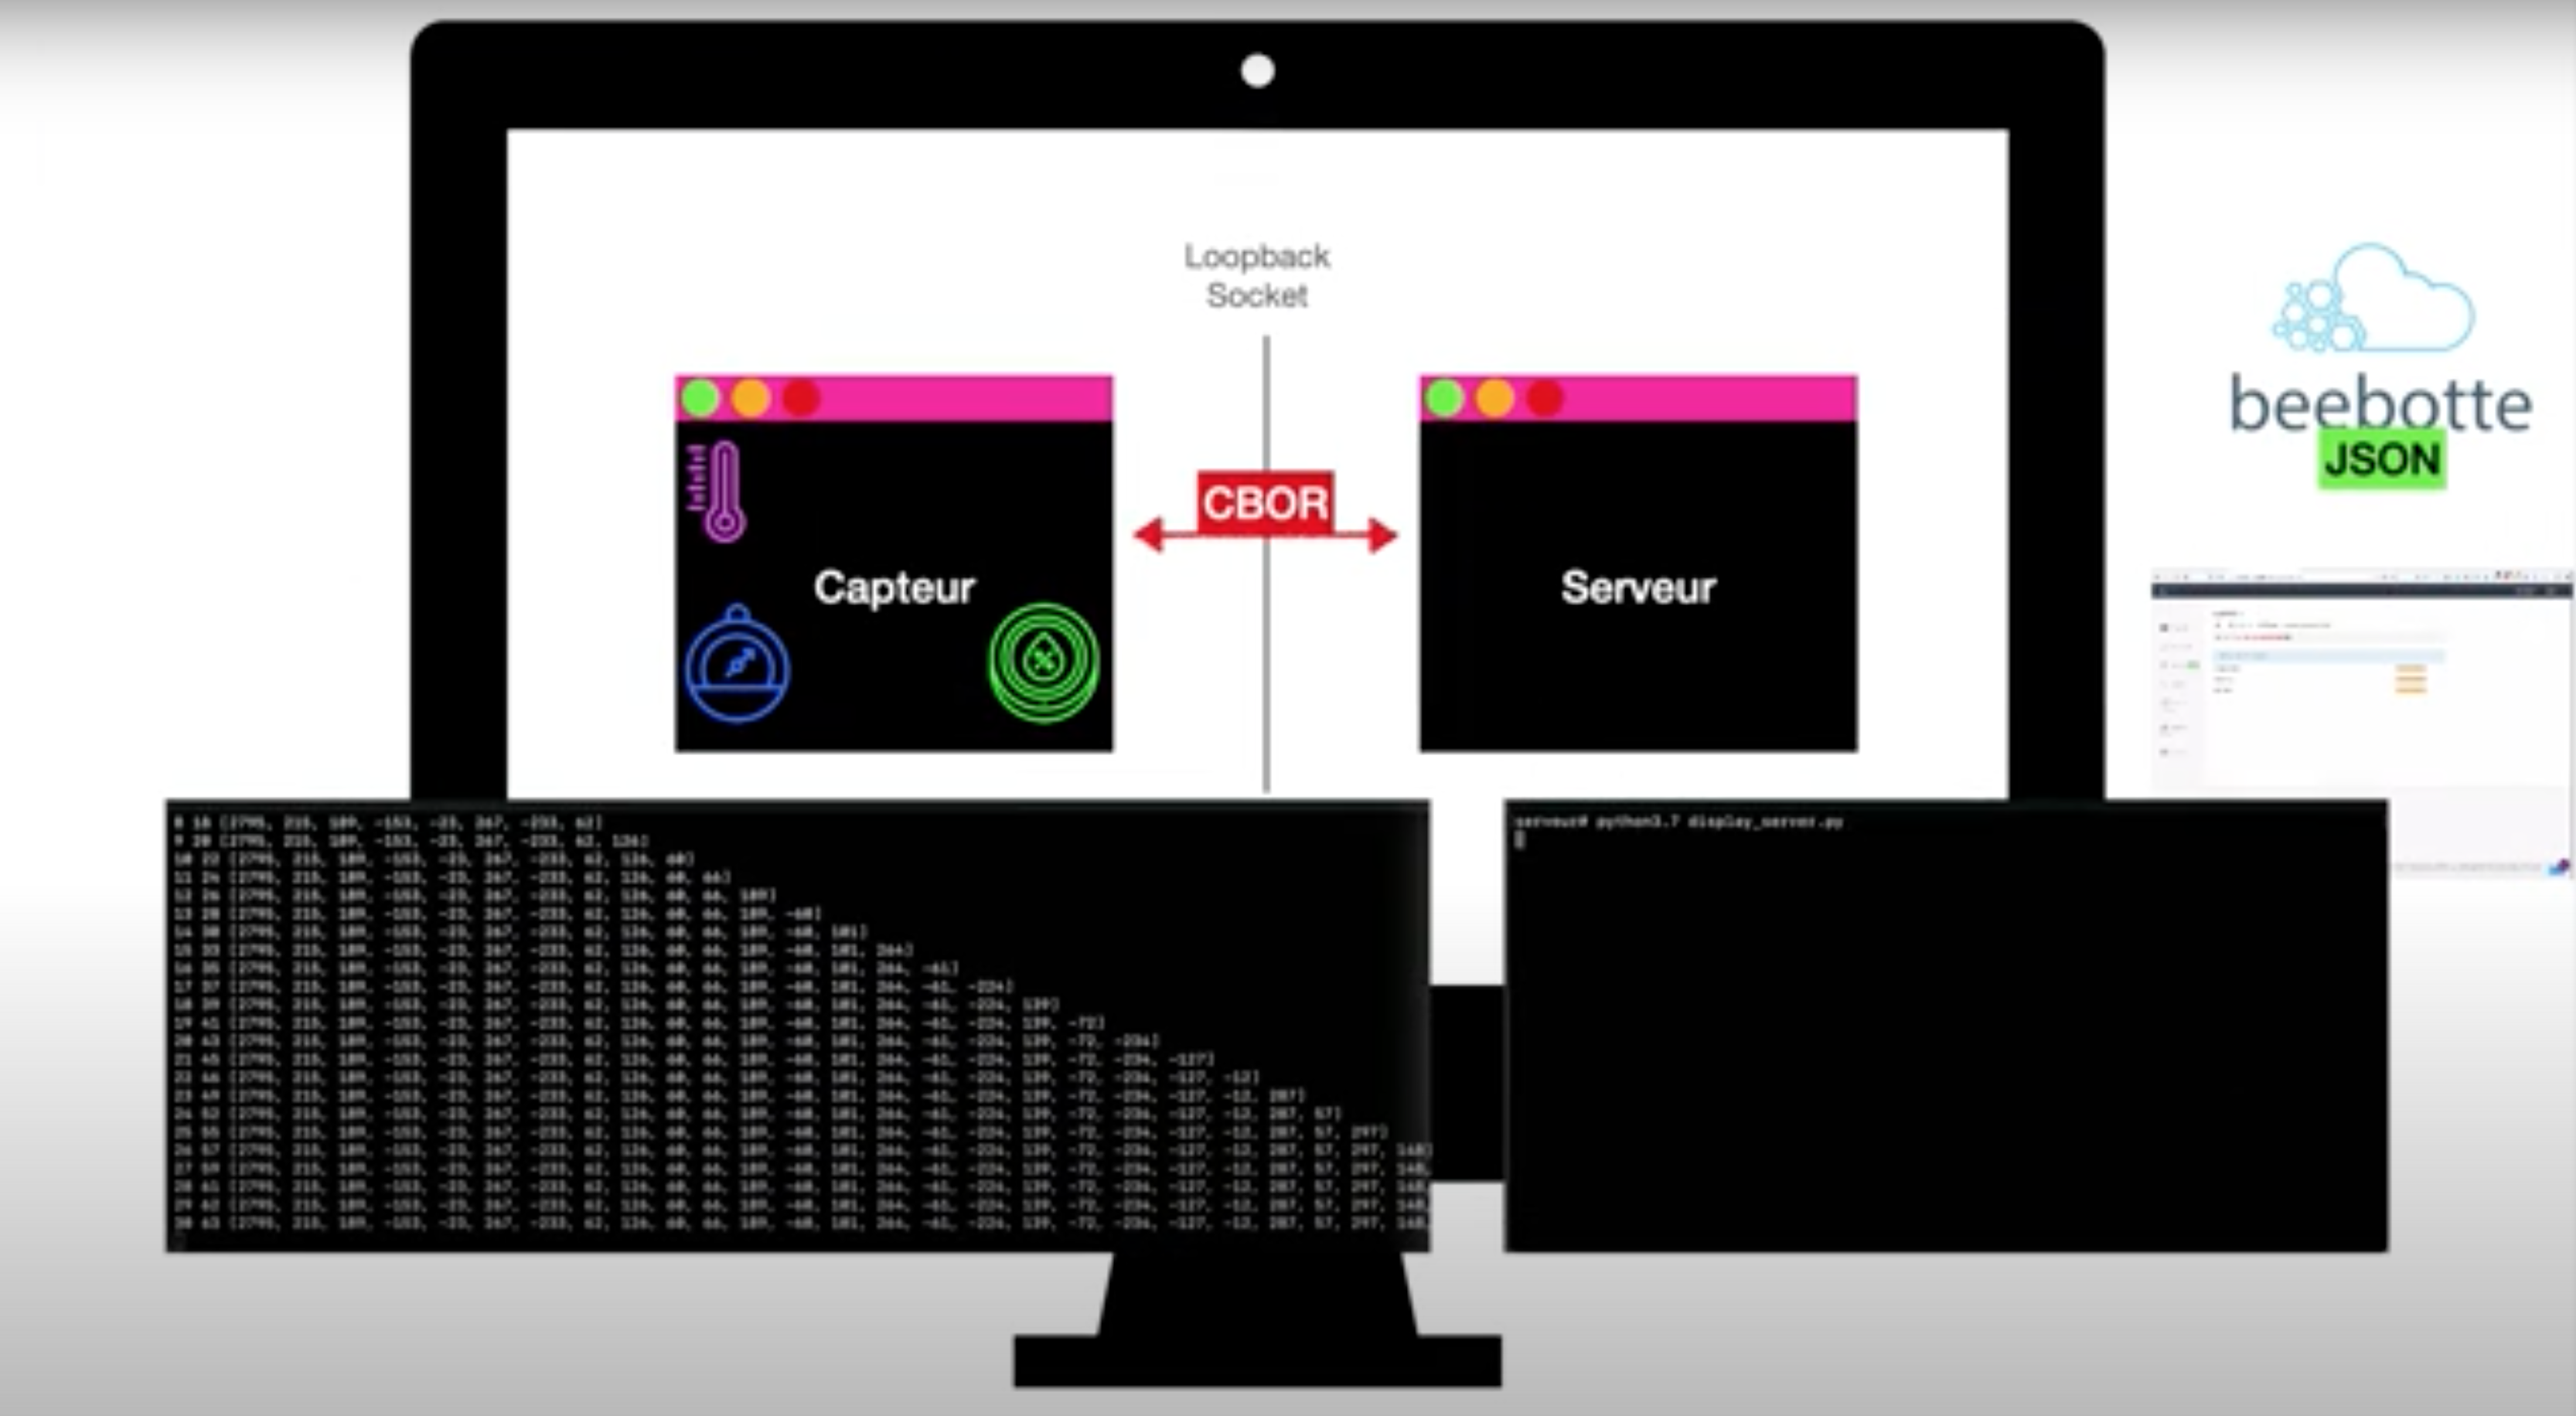
\includegraphics[width=1\columnwidth]{Pictures/Capture40.png}}
\caption{Architecture Client/Serveur}
\label{fig-client-serveur}
\end{figure}

\section{\Index{Beebotte}}

Il existe plusieurs sites qui permettent de le faire. Nous allons utiliser \url{https://beebotte.com}, mais ce que nous allons présenter peut très bien s'appliquer à d'autres sites.

\subsection{Configuration}

\begin{wrapfigure}{r}{3cm}

\includegraphics[width=.2\columnwidth]{Pictures/beebotte.png}
\end{wrapfigure}

La première étape consiste à créer un compte en cliquant sur \textit{Sign Up} sur la page de garde et en remplissant un formulaire classique avec votre login, adresse de courrier électronique et mot de passe. Une fois le compte validé, le service est accessible.

Le compte nous permet de nous authentifier pour gérer les données sur le site, mais il faut également disposer d’autorisation pour pouvoir y déposer des données via l’\Index{API REST}.
Pour cela, il faut se rendre sur la page \textit{Account Setting} puis l’onglet \textit{Access Management}. 
Cette page (cf. figure~\vref{fig-bb-key}) donne une clé et un secret pour gérer l’ensemble des données sur le site. 

\begin{figure}[tbp]
\centerline{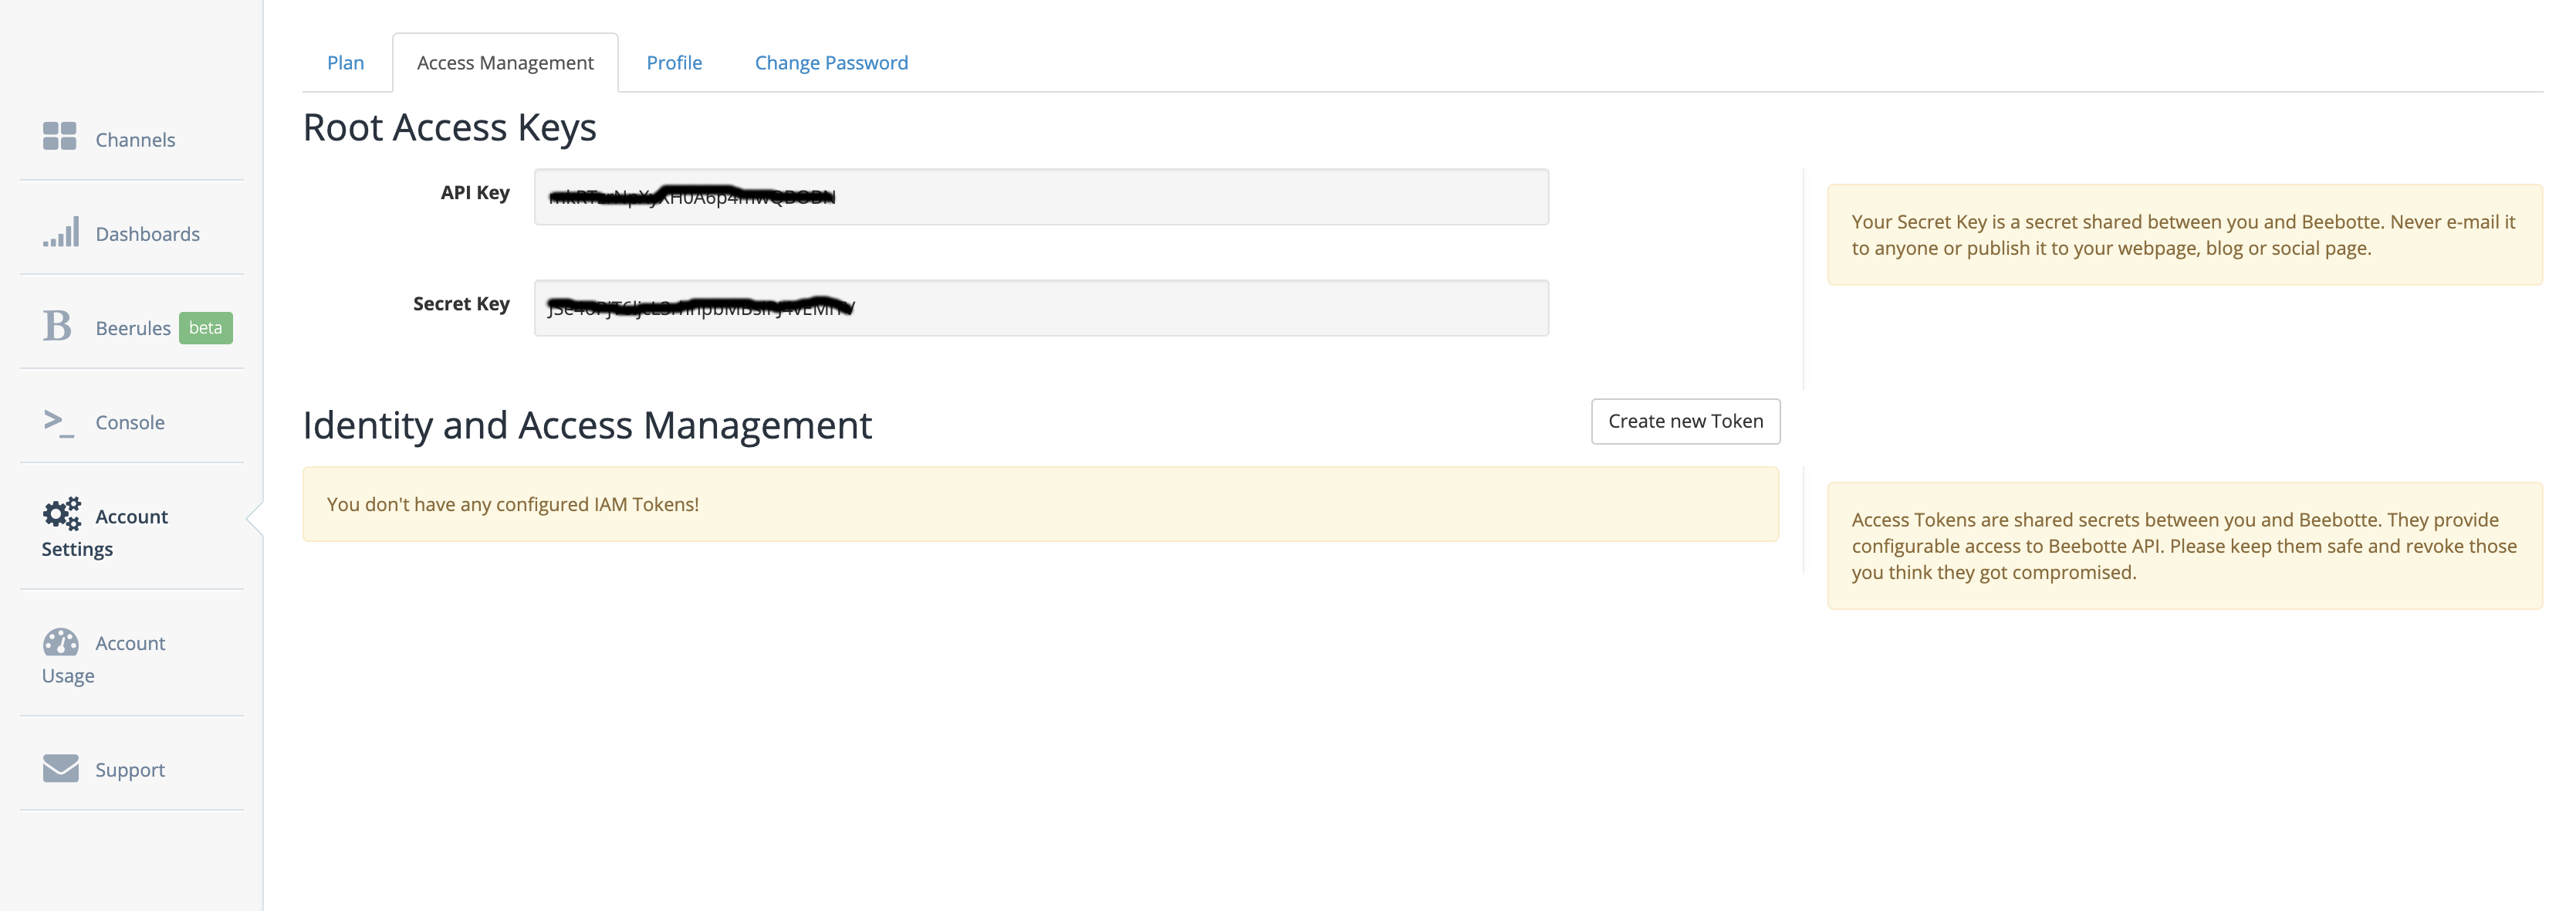
\includegraphics[width=1\columnwidth]{Pictures/bb_root_token.png}}
\caption{Clé et secret pour l'authentification}
\label{fig-bb-key}
\end{figure}


Notez ces valeurs et stockez les dans un fichier \pprog{config\_bbt.py} qui a cet aspect (vos valeurs sont forcément différentes) :

\pythonlst{config\_bbt.py}




Nous allons maintenant créer un canal (/textit{channel}) dans lequel nous allons définir les objets correspondant aux capteurs. En Cliquant sur \textit {Channels} puis \textit{Create New}, la page représentée figure~\vref{fig-new-channel} apparaît. 

Il faut donner un nom au channel (\textit{capteurs} dans l'exemple), cocher la case \textit{public} et créer trois ressources pour les trois valeurs qui nous intéressent (\textit{temperature}, \textit{humidity}, \textit{presure}) et faire correspondre les unités.



\subsection{Enregistrement des ressources}

Le programme \pprog{display\_server.py} permet de correspondre avec Beebotte via son API REST. Il commence par l'importation des modules nécessaires~:

\pythonlst[firstline=1,lastline=8, firstnumber=1]{display\_server.py}


\begin{itemize}
    \item ligne 4, le module Python \texttt{beebotte}  est disponible pour simplifier la manipulation des données\footnote{S'il n'était pas présent sur votre ordinateur, vous devriez l'installer avec la commande \texttt{pip3 install beebotte}.}.
    \item ligne 5, le module \texttt{contient} la clé et le secret nécessaire à la connexion obtenu précédemment.
    
\end{itemize}



\pythonnxt[firstline=9,lastline=11, firstnumber=9]{display\_server.py}

\begin{itemize}
    \item ligne 10 et 11 permette d'ouvrir la socket pour communiquer avec les capteurs.
\end{itemize}

\pythonnxt[firstline=12,lastline=14, firstnumber=12]{display\_server.py}


\begin{itemize}
    \item ligne 13 une instance permettant la connexion avec les serveurs de Beebotte est définie grâce à la fonction \pfunction{beebotte}{BBT}. Les paramètres de connexion provenant du module \texttt{config\_bbt} sont pris en compte. 
\end{itemize}


\pythonnxt[firstline=41,lastline=45, firstnumber=41]{display\_server.py}

Dans le programme principal, un boucle sans fin attend la série temporelle codée en CBOR venant du capteur (ligne 42), les transforme tableau Python (ligne 44) et appelle la fonction \texttt{to\_btt} en précisant\:
\begin{itemize}
    \item le canal et la ressource qui ont été définie précédemment sur Beebotte~;
    \item la série temporelle
    \item la précision pour transformer ces entiers en flottant.
\end{itemize}
.  

\pythonnxt[firstline=15,lastline=38, firstnumber=15]{display\_server.py}

La fonction \texttt{to\_bbt} fait l’essentiel du travail de transformation. Elle prend en argument :

\begin{itemize}
    \item le nom du canal créé sur Beebotte. Dans notre cas, ce sera \texttt{capteurs} ;
    \item le nom de l’objet dans ce canal que nous avons également créé sur le site web. Dans notre cas, ce sera \texttt{humidity} ;
    \item le tableau python des mesures codées en delta ;
    \item le facteur multiplicatif, c’est-à-dire la précision. Ici, il faudra diviser par 100 ;
    \item la période entre deux mesures ; cela nous permettra de calculer l’instant de la mesure. Par défaut, la période est de 10 secondes ;
    \item le temps de réception du message pour dater les échantillons. S’il n’est pas spécifié, le temps courant est pris.

\end{itemize}

       \vspace{1em}

Cette fonction transforme le tableau Python suivant :
\begin{termc}[backgroundcolor=\color{palerod},  basicstyle=\ttfamily\small, escapechar=\#]
[3311, 124, -144, -188, -94, 289, -1, -72, 1 ...
\end{termc}

en un tableau de dictionnaire :

\begin{termc}[backgroundcolor=\color{palerod},  basicstyle=\ttfamily\small, escapechar=\#]
[{'data': 33.11, 'resource': 'humidity', 'ts': 1596730115000.0},
 {'data': 34.35, 'resource': 'humidity', 'ts': 1596730125000.0},
 {'data': 32.91, 'resource': 'humidity', 'ts': 1596730135000.0},
 {'data': 31.03, 'resource': 'humidity', 'ts': 1596730145000.0},
 ...
\end{termc}

       \vspace{1em}

Chaque dictionnaire contient trois éléments imposés par Beebotte :

\begin{itemize}
\item le nom de la ressource (\texttt{resource}) telle qu'elle a été définie sur l’interface pour le canal ;
\item la valeur associée pour cette ressource (\texttt{data}) ;
\item l’instant à laquelle cette mesure a été faite (\texttt{ts}). Le temps est représenté suivant le format \Index{Epoch} qui compte le nombre de secondes depuis le premier Janvier 1970\footnote{voir \url{https://www.epochconverter.com/} pour les conversions.}.
\end{itemize}

       \vspace{1em}

Le calcul du \textit{timestamp} (\texttt{ts}) est l’opération la plus complexe de cette fonction mais les module \texttt{time} et \texttt{datetime} facilitent le calcul. 
Si l'argument \texttt{epoch} a été fourni lors de l'appel, la fonction prend cette valeur, sinon le calcule ligne 23. La fonction \pfunction{datetime}{now} retourne la date et l'heure courante, qui est transformé en un tuple grâce à la fonction \pfunction{datetime}{timetuple}. A partir de ce dernier, la fonction \pfunction{time}{maketime} le converti en epoch. 



Ligne 25, l'epoch à laquelle la première mesure du tableau a été faite est calculé en prenant le temps actuel (cela suppose que l’on néglige le temps de traitement et de transmission) auquel on retranche la durée de la capture, c’est-à-dire comme le nombre d’éléments du tableau multiplié par l’intervalle entre chaque mesure (\texttt{period}). 

Ligne 32 à 34 la structure attendue par Beebotte est construite. le résultat est envoyé, ligne 38, grâce à la fonction \pfunction{beebotte}{writeBulk} qui permet d'envoyer un ensemble de valeurs dans un tableau.

       \vspace{1em}

On peut vérifier que Beebotte a reçu des données en visualisant le canal capteurs sur l’interface Web. On peut voir sur la  figure~\vref{fig-bb-mesure} que seule la ressource \texttt{humidity} a reçu des données. L’interface affiche la dernière valeur reçue et la date de réception.

\begin{figure}[tbp]
\centerline{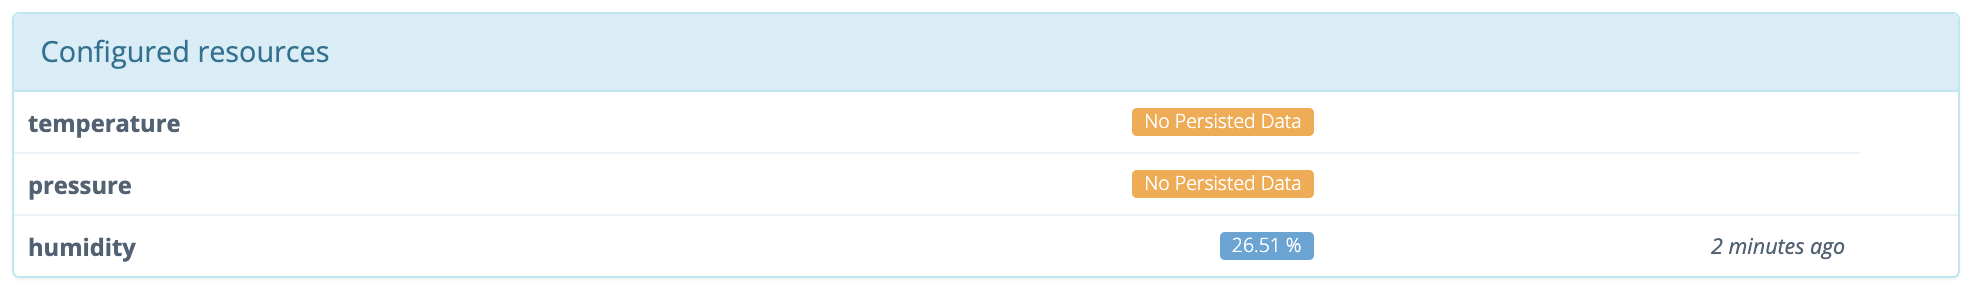
\includegraphics[width=1\columnwidth]{Pictures/bb_mesures.png}}
\caption{État des ressources}
\label{fig-bb-mesure}
\end{figure}

\subsection{Visualisation des ressources}

Maintenant que les ressources sont stockées dans les serveurs de Beebotte, il est possible de les visualiser graphiquement, en allant dans \textit{Dashboard} puis \textit{create Dashboard} et \textit {Add Widget} pour sélectionnez un widget comme \textit{Multi-line chart}.

 

Puis, configurez le widget en définissant le canal et la ressource de ce canal comme le montre la figure~\vref{fig-widget}.

\begin{figure}[tbp]
\centerline{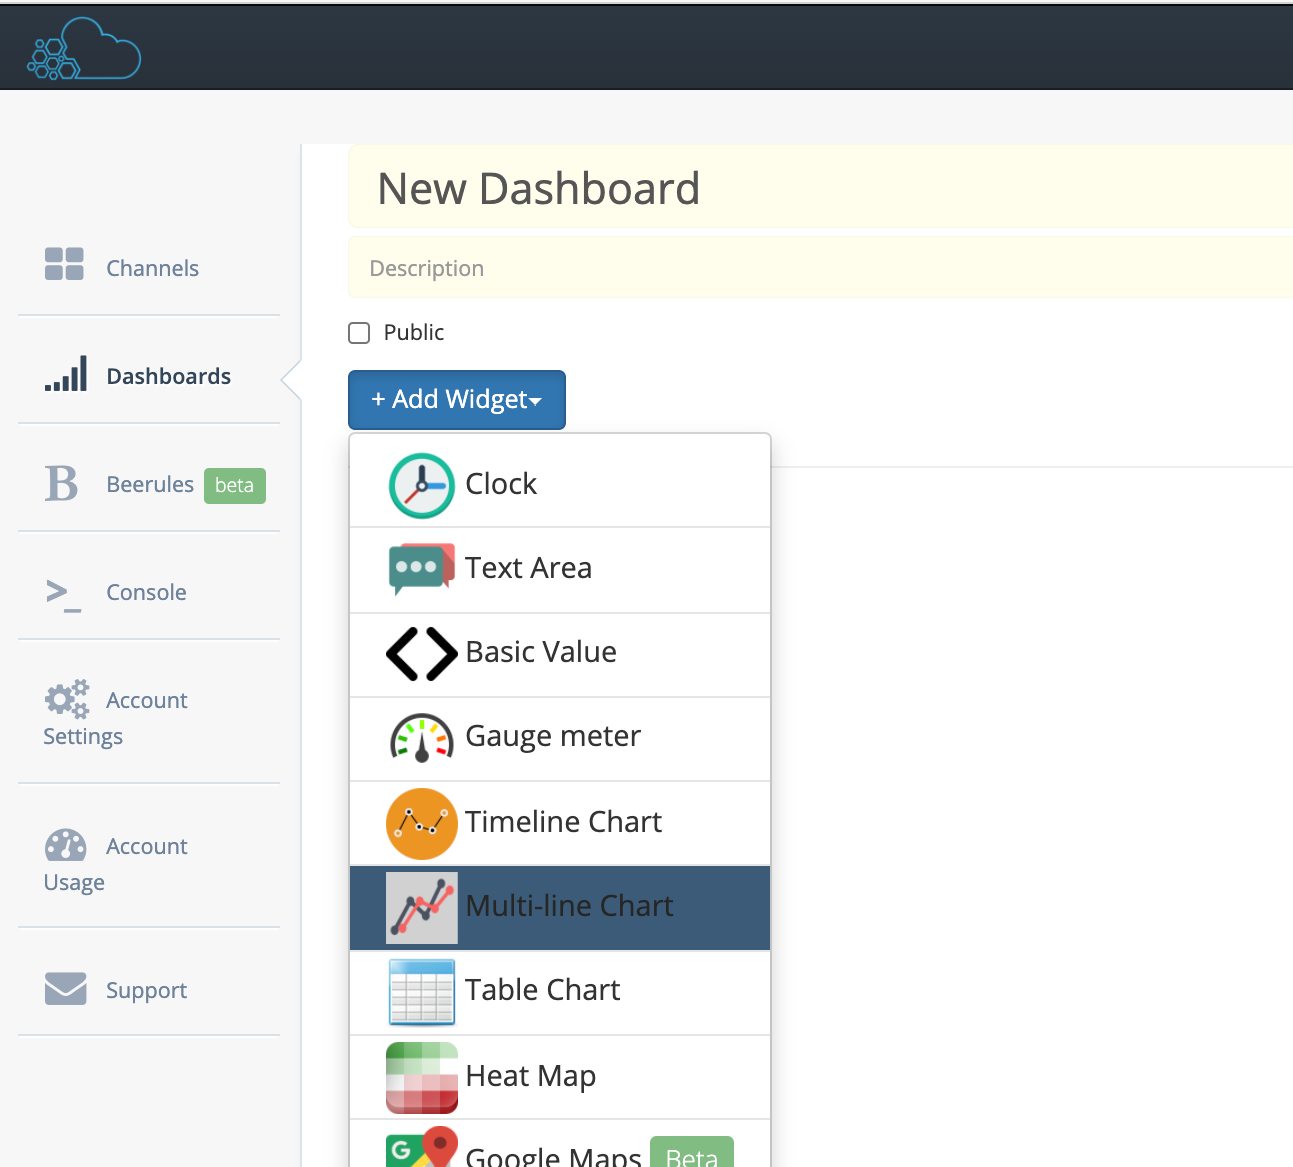
\includegraphics[width=0.5\columnwidth]{Pictures/bb_new_widget.png}}
       \vspace{1em}
\centerline{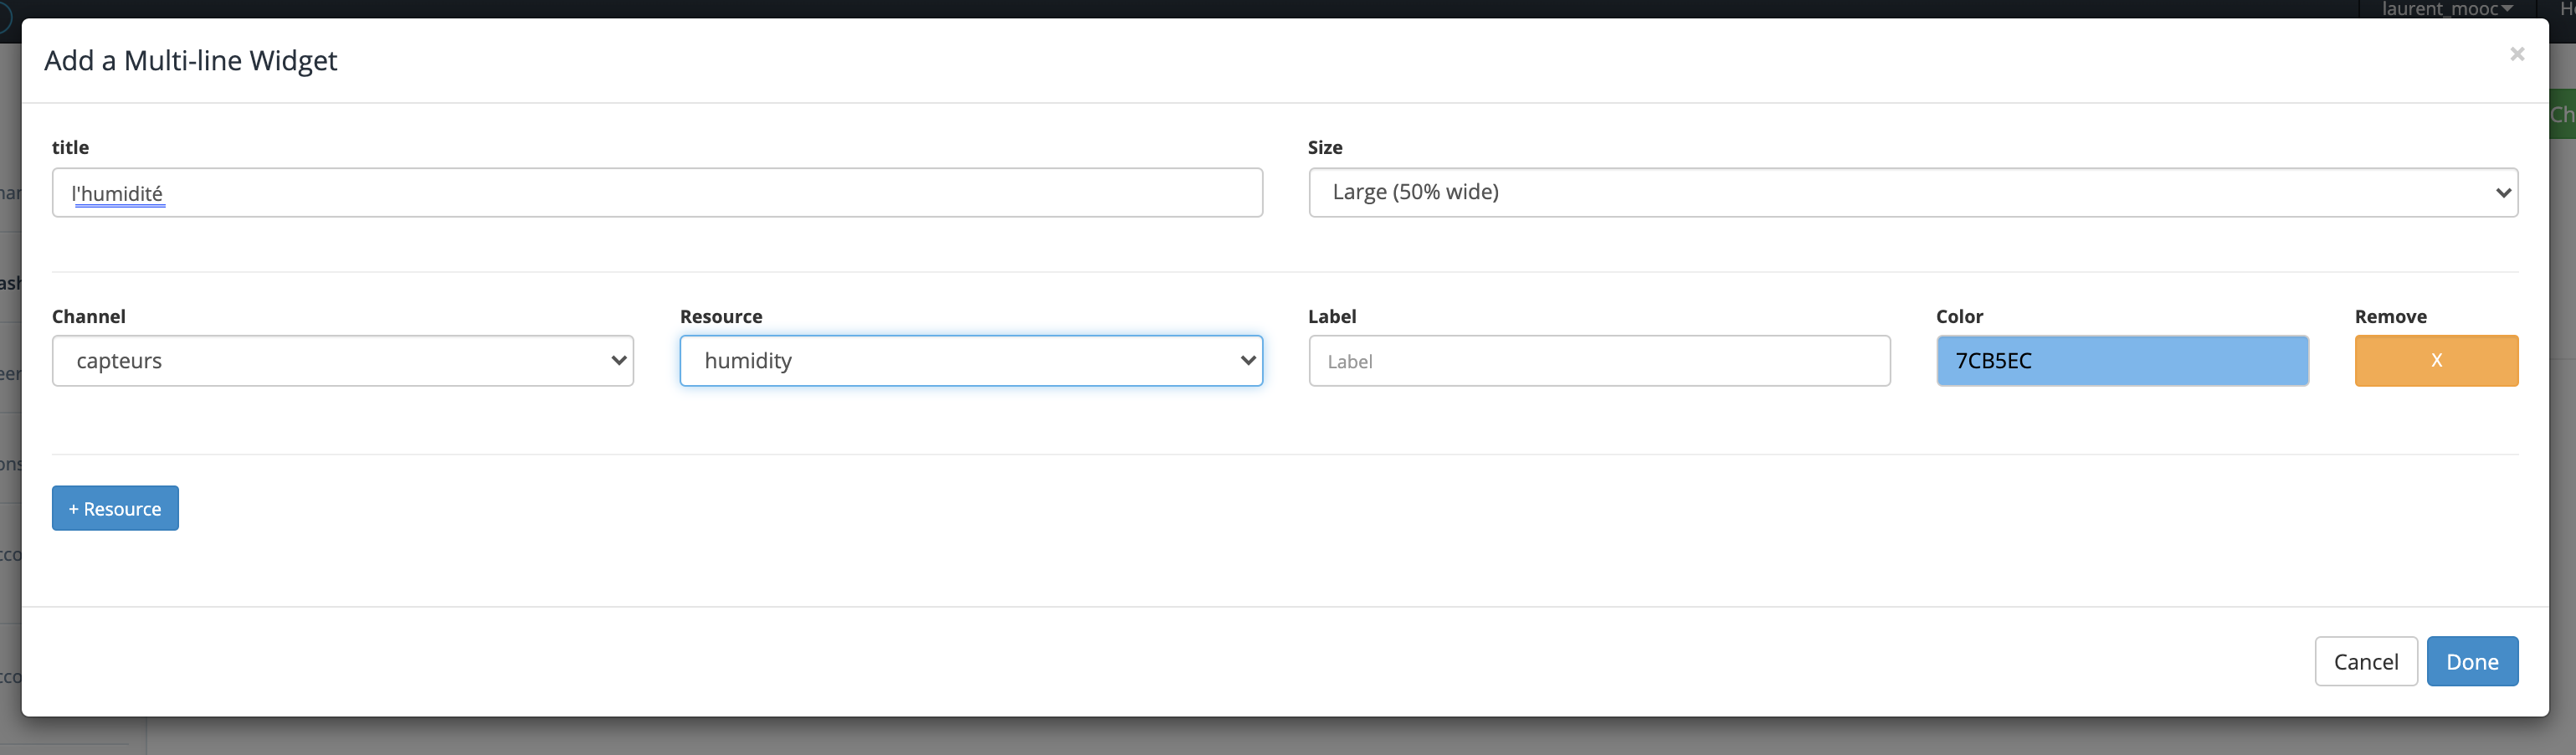
\includegraphics[width=0.5\columnwidth]{Pictures/bb_conf_widget.png}}
\caption{Création d'un widget}
\label{fig-widget}
\end{figure}


En retournant sur le dashboard, on peut voir l’évolution de l’humidité au cours du temps (cf. figure~\vref{fig-bb-humidity}). 

\begin{figure}[tbp]
\centerline{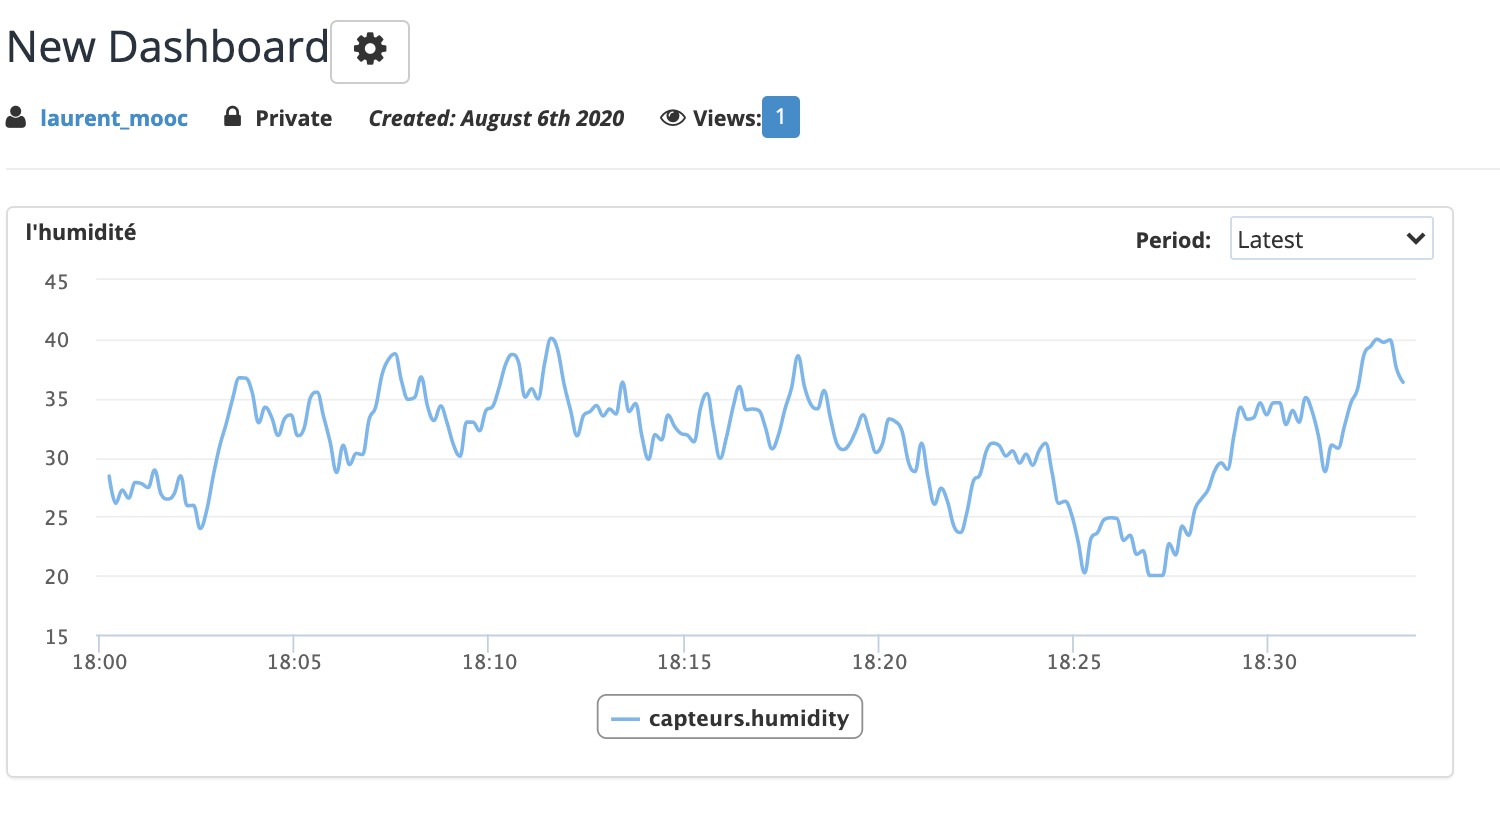
\includegraphics[width=1\columnwidth]{Pictures/bb_humidity.png}}
\caption{Suivi de l'humidité}
\label{fig-bb-humidity}
\end{figure}

\section{Interopérabilité}

La chaîne de collecte de l'information que nous venons de construire allant du capteur à l'affichage, n'est pas complètement interopérable. Certes le capteur envoie des données au format CBOR qui peuvent être interprété par l'autre extrémité, mais le récepteur ne sait pas~:
\begin{itemize}
    \item qu'il s'agit d'une série temporelle codée avec des deltas~;
    \item que les données ont été multipliée par 100 pour pouvoir envoyer des nombres entiers, plus compacts sans perdre trop de précision~;
    \item que le pas de mesure est de 10 secondes
    \item que les données concernent le taux d'humidité.
\end{itemize}

Ces informations ont été précisées dans le programme \pprog{display\_server.py}, de même la transformation de la structure de tableau de la série temporelle en un dictionnaire avec des mots clés spécifique à Beebotte on été gravé dans le programme. 

       \vspace{1em}

Nous verrons par la suite comment améliorer cette interopérabilité.

\section{et SenML ?}

Dans la communication avec Beebotte,  le site structure l’envoi des mesures en définissant un dictionnaire JSON avec des mots clés particuliers. Pour utiliser un autre site, le format des échanges doit êter modifié même si les informations restent identiques.

       \vspace{1em}

De plus, lors de la configuration des ressources sur le site de Beebotte, la nature de la mesure a du être précisée~; par exemple, s’il s’agit d’une température, d’un taux d’humidité... Il faut également parfois indiquer le type de la mesure (texte, entier, flottant...) voire les unités. 

       \vspace{1em}

\ac{SenML} défini dans le \rfc{8428} propose une structuration des données fournie par le capteur. 
Pour réduire l’impact de la transmission, les noms des champs ont été choisis pour être le plus compact possible. 
Par exemple, la lettre \texttt{v}  va indiquer une valeur (à comparer avec la clé \texttt{data} utilisée lors de la communication avec Beebotte). 
Pour être encore plus compact, la représentation en CBOR utilisera des entiers courts au lieu de caractères.

       \vspace{1em}

Il est également possible de transporter l’unité de la mesure avec le mot clé \texttt{u} .


SenML ne définit pas que des unités  du système international, mais également des unités secondaires pour limiter la taille de la représentation. Il sera plus compact de transmettre :

\begin{termc}[backgroundcolor=\color{palerod}, basicstyle=\ttfamily\small, escapechar=\#]
{"u": "MHz", "v": 868}
\end{termc}

que
\begin{termc}[backgroundcolor=\color{palerod},  basicstyle=\ttfamily\small, escapechar=\#]
{"u": Hz", "v": 868000000}.
\end{termc}

Le standard définit aussi des temps de base et des valeurs de base auxquelles les temps et les valeurs vont se référer ; ce qui permet également de réduire la taille des valeurs. Finalement, le ou les objets peuvent s’identifier dans les données transmises en définissant un nom de base (\texttt{bn} : \textit{base name}), le nom du capteur (\texttt{n} : \textit{name}) vient compléter le nom de base.

\subsubsection{Émission}

\pythonlst{minimal\_senml\_client.py}

Le programme \pprog{minimal\_senml\_client.py} illustre le fonctionnement de SenML. Il repose sur deux objets~:
\begin{itemize}
\item l'objet \pfunction{kpn\_senml}{SenmlPack} inclus les informations commune à l'objet, comme le nom de base (ici \texttt{device1} ligne 23) ou la base de temps, ligne 24.
\item l'objet \pfunction{kpn\_senml}{SenmlRecord} contient une mesure où l'on peut préciser son nom, son unité et sa valeur (lignes 32, 38 et 43). Le temps est également précisé ligne 35. Ces enregistrements sont ajoutés à l'objet \texttt{pack}.
\end{itemize}

Le programme récupère les trois valeurs de température, humidité et pression (lignes 27 à 29) en les arrondissant à 2 chiffres après la virgule pour la température et l'humidité et converti la pression, d'hecto Pascal en Pascal puisque c'est l'unité définie par SenML. 

Les mesures se font toutes les 10 seconde (délais ligne 48) et quand le nombre de mesures défini ligne 13 est atteint, le codage SenML en CBOR est envoyé au serveur. 

       \vspace{1em}

\begin{termc}[backgroundcolor=\color{palerod}, basicstyle=\ttfamily\small, escapechar=\#]
[{'bn': 'device1', 'bt': 1640110457.0,  
  'n': 'temperature', 't': 0.0, 'u': 'Cel',   'v': 19.98},
 {'n': 'humidity', 'u': '%RH', 'v': 28.46},
 {'n': 'pressure', 'u': 'Pa', 'v': 100093}]
JSON length:  177 bytes
CBOR length:  104 bytes
\end{termc}

Ce premier listing montre le premier enregistrement pour les trois grandeurs mesurées. Il s'agit d'un tableau de 3 éléments. Le premier contient les valeurs de bases (ici le nom et l'heure de référence) suivi de la grandeur à mesurer, de son unité et sa valeur. Le deuxième et le troisième éléments, mettent à jours le nom de la grandeur, son unité et sa valeur, les autres informations précédemment définies restent valables.


\begin{termc}[backgroundcolor=\color{palerod},  basicstyle=\ttfamily\small, escapechar=@]
[@\textcolor{gray}{\{'bn': 'device1',  'bt': 1640110457.0,}@
 @\textcolor{gray}{ 'n': 'temperature',  't': 0.0, 'u': 'Cel', 'v': 19.98\},}@
 @\textcolor{gray}{\{'n': 'humidity', 'u': '\%RH', 'v': 28.46\},}@
 @\textcolor{gray}{\{'n': 'pressure', 'u': 'Pa', 'v': 100093\},}@
 {'n': 'temperature', 't': 10.0, 'u': 'Cel', 'v': 20.03},
 {'n': 'humidity', 'u': '%RH', 'v': 26.86},
 {'n': 'pressure', 'u': 'Pa', 'v': 100065}]
JSON length:  318 bytes
CBOR length:  188 bytes
 \end{termc}
 
 Quand on ajoute 10 secondes plus tard de nouvelles mesures,  un temps relatif de 10 secondes est indiqué pour l'enregistrement des températures et il reste valable pour les enregistrements suivants.
 
 \Question{codage}
 {A quoi correspond la clé \texttt{'u' : 'Cel'} que l'on retrouve dans la structure précédente ? }
 {Unité = degrés Celcius}
 
 \Question{Accroissement}
 {Dans les deux représentations JSON et CBOR, de combien la taille est-elle accrue par l'ajout des mesures effectuées ? d'où viennent ces différences ?}
 {
 Si l'on regarde le listing précédent, l'ajout des trois mesures fait augmenter la taille de 141 octets pour JSON et 84 pour CBOR. La différence vient de l'utilisation de nombre plus que de chaînes de caractères pour les clés. Ainsi 't' demande 3 caractères en JSON avec les guillemets, codé en CBOR, il faudrait 2 octets, un nombre inférieur à 23 se code sur un seul octet. Il y a egalement les virgules, espaces et fermeture de crochets qui ne sont pas présent en CBOR. Les nombres flottant comme \texttt{19.98} ont une représentation plus compacte en JSON (5 octets) qu'en CBOR où ils consomment 9 octets. Dans tous les cas l'accroissement est fortement dépendant du nom des éléments. Ici, il faut répéter à chaque fois \texttt{temperature}, \texttt{humidity} et \texttt{pressure}, soit 26 caractères.
 }
 
 \Question {Une seule grandeur}
 {Si on ne s'intéressait qu'à une seule grandeur, par exemple l'humidité. A quoi ressemblerait la structure SenML en JSON ?}
 {
 Chaque nouvelle entrée ajoute 35 octets à la structure~: 
 [\{'bn': 'device1',  'bt': 1640110457.0, 'n': 'humidty', 'u': '\%RH', 'v': 28.46\},\\
 \{'t': 10.0, 'v': 26.86\},\\
 \{'t': 20.0, 'v': 26.96\},\\
 \{'t': 30.0, 'v': 27.01\}]\\
 }
 
 \subsubsection{Réception}
 
 Le traitement par le module SenML tel qu'il est mis en œuvre n'est pas complet, il ne gère pas correctement les timestamps. Mais, il n'est pas vraiment nécessaire pour traiter ces messages. En effet, comme on l'a vu précédemment, les objets SenML sont cumulatifs, une clé reste présente dans les enregistrements suivants sauf si elle est redéfinie. 
 
 
 \pythonlst{minimal\_senml\_server.py}
 
 Le programme \pprog{minimal\_senml\_server.py} va convertir le format SenML codé en CBOR dans le format attendu par Beebotte. 
 La version CBOR utilise ds nombres plutôt que des tags.
 Le dictionnaire \texttt{naming\_map} defini lignes 10 à 12 permet la correspondance utilisé par la suite pour rendre le code plus lisible.
 
 Les lignes 14 à 17 initialisent les communications venant du capteur et celles allant à Beebotte. 
 
 Les données reçues ligne 21 sont transformée en structure Python ligne 23. Cette correspondance est possible car Python autorise des clés numériques et celles-ci ne sont pas répétées plusieurs fois dans une map CBOR.
 
La boucle commençant ligne 28 permet d'explorer tous les éléments du tableau SenML, les nouvelles entrées sont fusionnées avec les anciennes (ligne 29)\footnote{Dans les version plus récentes de Python, il est possible d'utiliser l'opérateur \texttt{|}.}. 

Les informations concernant le temps sont ensuite recherchées. 
D'abord le temps (ligne 32) et s'il un temps de base existe (ligne 33) il est ajouté. On procède de même pour la valeur (lignes 38 à 40). Pour le nom, il n'y a pas de concaténation car le nom de base sera utilisé comme canal Beebotte, il est récupéré à la fin ligne 46.

A partir de ces informations, la structure attendue par Beebotte est construite ligne 43 en ajoutant le dictionnaire dans le tableau \texttt{bbt\_record}.

Ligne 47, l'information est envoyée à Beebotte. Si les clés d'authentification, le nom du canal et des ressources sont correct, les information s'affiche sur le site, comme précédemment. 

\begin{termc}[backgroundcolor=\color{palerod},  basicstyle=\ttfamily\tiny, escapechar=@]
{0: 'temperature', 1: 'Cel', 2: 19.44, 6: 0.0, -3: 1640168049.0, -2: 'device1'}
{0: 'humidity', 1: '%RH', 2: 24.13, 6: 0.0, -3: 1640168049.0, -2: 'device1'}
{0: 'pressure', 1: 'Pa', 2: 101080, 6: 0.0, -3: 1640168049.0, -2: 'device1'}
{0: 'temperature', 1: 'Cel', 2: 19.48, 6: 10.0, -3: 1640168049.0, -2: 'device1'}
{0: 'humidity', 1: '%RH', 2: 21.85, 6: 10.0, -3: 1640168049.0, -2: 'device1'}
{0: 'pressure', 1: 'Pa', 2: 101090, 6: 10.0, -3: 1640168049.0, -2: 'device1'}
{0: 'temperature', 1: 'Cel', 2: 19.57, 6: 20.0, -3: 1640168049.0, -2: 'device1'}
{0: 'humidity', 1: '%RH', 2: 21.09, 6: 20.0, -3: 1640168049.0, -2: 'device1'}
{0: 'pressure', 1: 'Pa', 2: 101058, 6: 20.0, -3: 1640168049.0, -2: 'device1'}
{0: 'temperature', 1: 'Cel', 2: 19.52, 6: 30.0, -3: 1640168049.0, -2: 'device1'}
{0: 'humidity', 1: '%RH', 2: 20.39, 6: 30.0, -3: 1640168049.0, -2: 'device1'}
{0: 'pressure', 1: 'Pa', 2: 101120, 6: 30.0, -3: 1640168049.0, -2: 'device1'}
{0: 'temperature', 1: 'Cel', 2: 19.44, 6: 40.0, -3: 1640168049.0, -2: 'device1'}
{0: 'humidity', 1: '%RH', 2: 21.94, 6: 40.0, -3: 1640168049.0, -2: 'device1'}
{0: 'pressure', 1: 'Pa', 2: 101128, 6: 40.0, -3: 1640168049.0, -2: 'device1'}
[{'data': 19.44, 'resource': 'temperature', 'ts': 1640168049000.0},
 {'data': 24.13, 'resource': 'humidity', 'ts': 1640168049000.0},
 {'data': 101080, 'resource': 'pressure', 'ts': 1640168049000.0},
 {'data': 19.48, 'resource': 'temperature', 'ts': 1640168059000.0},
 {'data': 21.85, 'resource': 'humidity', 'ts': 1640168059000.0},
 {'data': 101090, 'resource': 'pressure', 'ts': 1640168059000.0},
 {'data': 19.57, 'resource': 'temperature', 'ts': 1640168069000.0},
 {'data': 21.09, 'resource': 'humidity', 'ts': 1640168069000.0},
 {'data': 101058, 'resource': 'pressure', 'ts': 1640168069000.0},
 {'data': 19.52, 'resource': 'temperature', 'ts': 1640168079000.0},
 {'data': 20.39, 'resource': 'humidity', 'ts': 1640168079000.0},
 {'data': 101120, 'resource': 'pressure', 'ts': 1640168079000.0},
 {'data': 19.44, 'resource': 'temperature', 'ts': 1640168089000.0},
 {'data': 21.94, 'resource': 'humidity', 'ts': 1640168089000.0},
 {'data': 101128, 'resource': 'pressure', 'ts': 1640168089000.0}]
 \end{termc}
 
 Le listing précédent montre cette transformation.
 Les premières lignes correspondent aux enregistrements fusionnées et le tableau final, ce qui a été envoyé à Beebotte.
 
 \Question{base value}
 {
 Pourrait-on utiliser le champ SenML \textit{base value} pour diminuer la taille des données de pression atmosphérique~?
 }
 {
Cela serait possible, si cette ressource était envoyée seule.
 }
%\chapter{Découvrons le LoPy}

\textit{Les programmes relatifs à cette section se trouvent dans le répertoire \texttt{plido-tp3} pour le serveur et \texttt{pycom} pour le LoPy.}

\section{Introduction}

Grâce aux émulateurs de capteurs décrits au chapitre précédent, vous avez pu appliquer les concepts essentiels de l'IoT sur votre ordinateur.

Cependant, si vous le pouvez, nous vous invitons à le faire sur de vrais objets connectés en utilisant des \Index{LoPy4} (plateforme de prototypage IoT) de la société \Index{Pycom} et des capteurs de température, humidité et pression \Index{BME280} (cf. figure~\vref{fig-lopy-bme280}). 

\begin{figure}[tbp]
\centerline{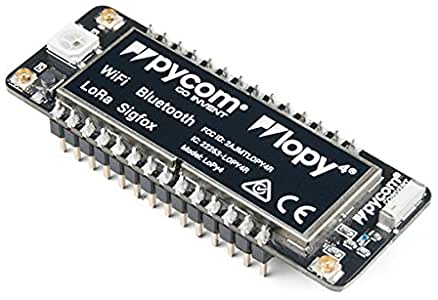
\includegraphics[width=.5\columnwidth]{Pictures/LoPy.jpg}  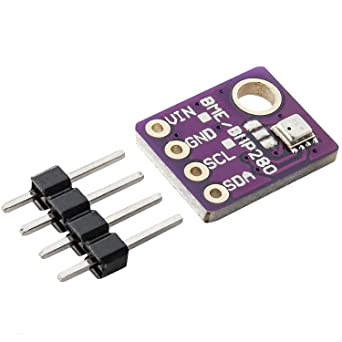
\includegraphics[width=.3\columnwidth]{Pictures/BME280.jpeg}}
\caption{LoPY4 et capteur BME280}
\label{fig-lopy-bme280}
\end{figure}

Un LoPY4 se programme en Python (ou plutôt \Index{MicroPython} qui est la version du langage pour systèmes embarqués) pour traiter les données. Dans un premier temps, nous allons utiliser le Wi-Fi pour communiquer avec votre ordinateur mais, par la suite, nous mettrons en place une communication via \Index{LoraWAN} ou \Index{Sigfox} qui peut vous demander plus de configuration mais vous permettra de mieux comprendre ces protocoles.

     \vspace{1em}


Même si vous n’avez pas de LoPy4, vous pouvez parcourir cette section pour voir les contraintes supplémentaires liées aux objets connectés.

\section{Installation d'Atom}

\Index{Atom} est un éditeur de texte performant, spécifiquement conçu pour le codage en différents langages. 
Atom va nous aider à programmer en Python et va également gérer la communication avec notre LoPy via le port \Index{USB} (grâce au plugin \Index{pymakr}). Atom fonctionne à peu près de la même manière sur \Index{Mac OS}, \Index{Windows} et \Index{Linux}, mais en s’adaptant aux particularités du système d’exploitation (place dans les menus, nom des liens séries...). Donc, il se peut que vous ayez quelques différences entre ce que vous avez dans cet ouvrage et l’écran de votre ordinateur. Les menus et sites Web indiqués peuvent également changer au cours du temps même si nous nous efforçons de faire des mises à jour régulières du cours.


     \vspace{1em}

Pour commencer à programmer avec votre LoPy, vous devez installer sur votre ordinateur le logiciel Atom (voir sur \url{http://atom.io}). Vous pouvez télécharger le package correspondant à votre système d'exploitation (cf. figure suivante).

\begin{figure}[tbp]
\centerline{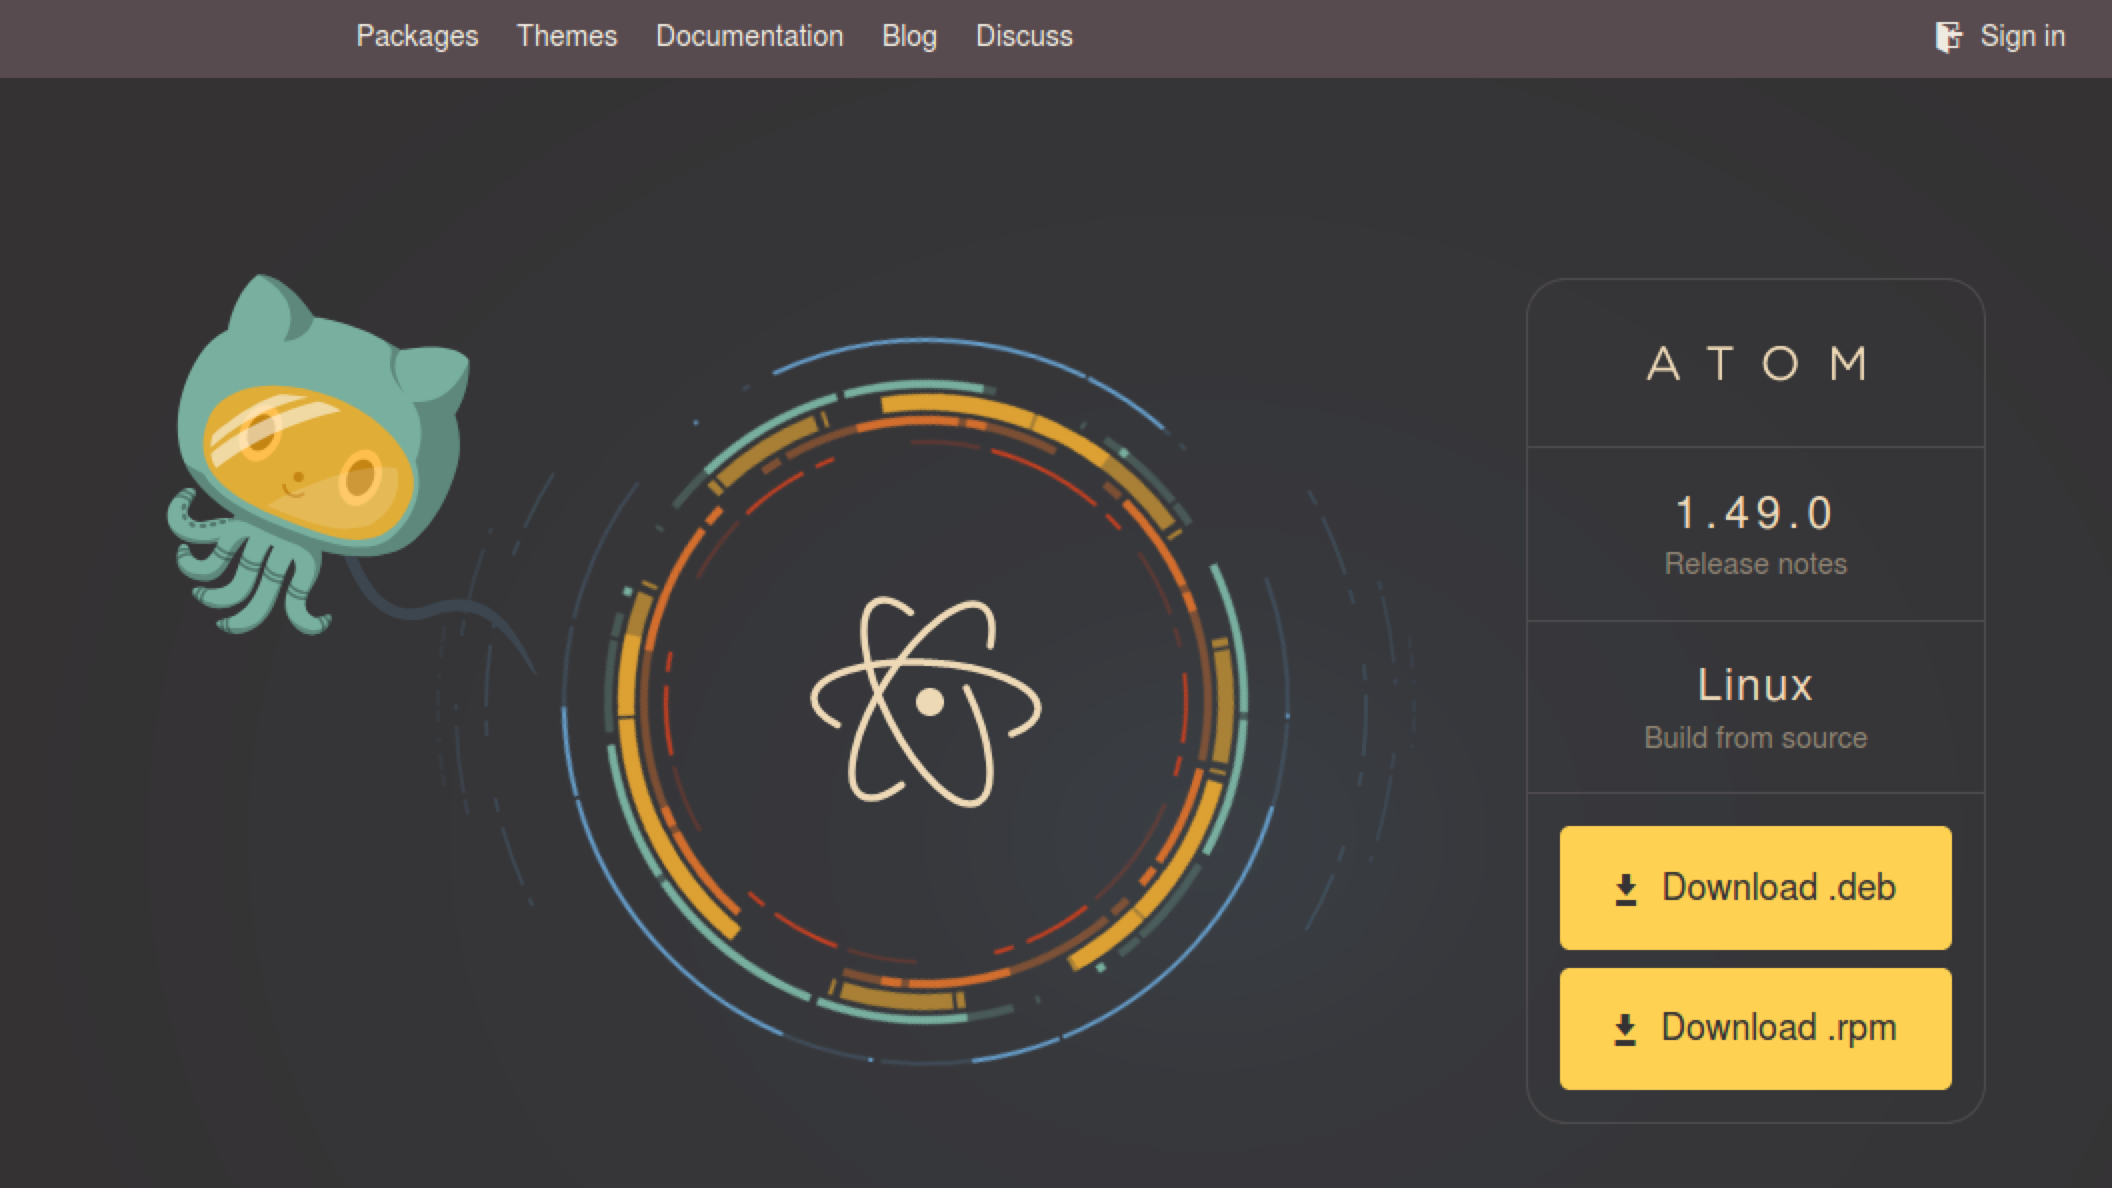
\includegraphics[width=1\columnwidth]{Pictures/atom_dl.png}}
\caption{Page d'accueil d'Atom}
\label{fig-page-atom}
\end{figure}
\begin{itemize}
\item Pour Mac et Windows, cliquez sur l’icône "télécharger" pour l’installer\footnote{il y a des risques d'incompatibilité des dernières versions d'Atom avec le package de gestion du LoPy (pymakr). Nous vous recommandons d'utiliser une version plus ancienne, comme la 1.43 disponible dans les archives d'Atom Release \url{https://github.com/atom/atom/releases/tag/v1.43.0}(\texttt{AtomSetup-x64.exe} pour Windows ou \texttt{atom-mac.zip} pour Mac OS).}.
\item Pour Linux, téléchargez le\texttt{.deb} et tapez \texttt{sudo dpkg -i atom-amd64.deb}\footnote{Il est possible qu'un message vous dise que git n'est pas installé. Dans ce cas, tapez \texttt{sudo apt-get install git} et suivez les instructions).}.
Lancez Atom en cliquant sur l’icône ou, sous Linux, en tapant atom dans un terminal.
\end{itemize}

     \vspace{1em}

Lancez Atom en cliquant sur l’icône ou, sous Linux, en tapant atom dans un terminal. L’écran d’accueil apparaît.

\subsection{Communiquez avec votre Pycom}

Pour communiquer avec le Pycom à travers Atom, vous devez installer le package pymakr.

Cliquez sur \textit{Install a Package} puis \textit{Open Installer}. Une autre fenêtre s’ouvre (cf. figure~\vref{fig-page-pakage}. Tapez \texttt{pymakr} dans le menu. Un package apparaît portant ce nom. Cliquez sur \textit{Install}. L’installation peut prendre plusieurs minutes. Vous avez le temps de prendre un café.

\begin{figure}[tbp]
\centerline{\includegraphics[width=1\columnwidth]{Pictures/atom_pymakr.png}}
\caption{Installation de Paquetages}
\label{fig-page-pakage}
\end{figure}

     \vspace{1em}

Une fois le café bu et l’installation terminée, une nouvelle fenêtre (terminal) s’ouvre en bas d’Atom.

     \vspace{1em}

Ce terminal (cf.figure~\vref{fig-page-pymakr}) vous permettra de dialoguer avec le LoPy. Branchez le LoPy à votre ordinateur. Vous devriez voir l’invite\texttt{ >{}>{}>{}} caractéristique d’un interpréteur Python\footnote{Sous Linux, vous devez être membre du groupe dialout pour pouvoir gérer la communication sur le port USB. Si vous ne voyez par l’invite, tapez sudo adduser login dialout en remplaçant login par le nom de votre compte Linux. Reconnectez-vous sous votre compte.}.

     \vspace{1em}

\begin{figure}[tbp]
\centerline{\includegraphics[width=1\columnwidth]{Pictures/atom_pymakr1.png}}
\caption{Fenêtre Pymakr}
\label{fig-page-pymakr}
\end{figure}

Toutes les commandes que vous allez taper dans cette fenêtre vont s’exécuter sur votre LoPy. Par exemple, si vous tapez\footnote{Les fenêtres sur fond gris montrent le code micropython et leur résultat.}~:

\begin{termc}[backgroundcolor=\color{gray!10}, language=json, basicstyle=\ttfamily\small, escapechar=@]
Connecting to /dev/ttyUSB0...
>>> @\textbf{1+1}@
2
>>>
\end{termc}

L’addition se fait sur le LoPy.

     \vspace{1em}

Sur le coté gauche de la fenêtre pymakr, plusieurs icônes sont présentes~:
\begin{itemize}
    \item l'interrupteur permet d'activer ou de désactiver le connexion avec le LoPy~;
    \item le triangle permet d'exécuter le programme affiché dans la fenêtre d'Atom sur le LoPy~;
    \item la flèche vers le haut, permet de recopier le répertoire actif dans la mémoire du LoPy. Cela sera utile pour installer de nouveaux modules sur le LoPy~;
    \item inversement le flèche vers le bas, permet de recopier la mémoire du LoPy sur l'ordinateur~;
    \item le processeur permet d'avoir des informations sur le loPy.
\end{itemize}

     \vspace{1em}

Sur la partie droite, l'onglet vertical \textit{Setting} permet de modifier les paramètres de connexion avec le LoPy.

\subsection{Installez votre environnement de travail} 

Pour programmer le LoPy, il faut récupérer les modules micropython. Le dépôt ca être téléchargé dans le répertoire de votre choix :

\begin{termc}[backgroundcolor=\color{gray!10}, language=json, basicstyle=\ttfamily\small, escapechar=@]
> git clone https://github.com/ltn22/PLIDObis.git
\end{termc}

Dans le menu \textit{Files>Open Folder} d’Atom, sélectionnez le répertoire \texttt{pycom} du dépot téléchargé, et validez. Sur la partie gauche de l’écran, l’ensemble des fichiers composant ce répertoire apparaissent. Il y en a beaucoup, car ils vont nous servir par la suite.

     \vspace{1em}

En cliquant dans la fenêtre \textit{\Index{pymakr}} sur le bouton \texiit{Upload project to device}, les fichiers de ce répertoire vont être copiés dans la mémoire du LoPy. Par la suite, si un module est modifié, il devra être resynchronisé dans la mémoire du LoPy.

\section{Connexion au réseau Wi-Fi}

\begin{wrapfigure}{r}{3cm}
\Youtube{https://youtu.be/PmvSU8AWO68}
\end{wrapfigure}


Pour rattacher de LoPY à un réseau \Index{Wi-Fi}, il doit dans un premier temps être configuré via la liaison USB de l'ordinateur pour lui donner les paramètres nécessaires à la connexion. 


Le fichier \texttt{\Index{boot.py}} a été copié lors du téléversement des fichiers dans la mémoire du LoPy. Au démarrage du LoPy, ce programme va chercher à se connecte à un réseau Wi-Fi. Comme le nom du réseau et la clé sécrète n'ont pas été founie, il n’y arrive pas. Le LoPy se transforme  en point d’accès. Au démarrage, le LoPy a dû afficher le message suivant, indiquant que le LoPy devient point d'accès Wi-Fi et va déployer son propre réseau sur lequel votre ordinateur peut se connecter. Le nom de ce réseau de les la forme \texttt{PLIDO\_XXXX} où \texttt{XXXX} est une séquence hexadécimal propre à l'équipement. La clé est \texttt{www.pycom.io}. Le LoPy à l'adresse \texttt{192.168.4.1} sur ce réseau.  

\begin{termc}[backgroundcolor=\color{gray!10}, language=json, basicstyle=\ttfamily\small, escapechar=@]
Failed to connect to any known network, going into AP mode
To connect look for 'PLIDO_5bac' access point, key = 'www.pycom.io'
\end{termc}

Mais ce n'est pas très intéressant car votre ordinateur va perdre sa connexion à l'internet. Pas très pratique pour suivre le MOOC. Avant d'afficher ce message, le LopY a montré la liste des réseaux Wi-Fi qu'il a détecté. Vous pouvez à l'inverse le connecter à un de ces réseau en renseignant le fichier \texttt{wifi\_conf.py} qui se trouve dans le répertoire \texttt{pycom}.


\pycomlst{wifi\_conf.py}

\texttt{MON\_SSID} doit être remplacé par le nom du réseau Wi-Fi ou \ac{SSID} et \texttt{MON\_MOT\_DE\_PASSE} par la clé qui y est associée. Notez que plusieurs réseaux Wi-Fi peuvent être ajouté, puisque \texttt{MON\_SSID} est vu comme une clé de l'objet JSON. L'édition de fichier s'est faite sur l'ordinateur, il doit être recopié dans la mémoire du LoPy en cliquant sur la flèche vers le haut.

Le Pycom redémarre et doit maintenant afficher un message du genre :

\begin{termc}[backgroundcolor=\color{gray!10}, language=json, basicstyle=\ttfamily\small, escapechar=@]
net to use ['MONWIFI']
Connected to MONWIFI with IP address: @\ul{192.168.1.76}@
Pycom MicroPython 1.20.2.r1 [v1.11-a5aa0b8] on 2020-09-09; LoPy4 with ESP32
Type "help()" for more information.
>>> 
\end{termc}



Il est possible de pinguer ou de se connecter avec \Index{FTP} ou \Index{telnet} en utilisant cette adresse IP.

\begin{termc}[backgroundcolor=\color{palerod}, language=json, basicstyle=\ttfamily\small, escapechar=@]
# @\textbf{telnet \ul{192.168.1.76}}@
Trying 192.168.1.86...
Connected to 192.168.1.86.
Escape character is ’ˆ]’.
MicroPython v1.8.6-760-g90b72952 on 2017-09-01; LoPy with ESP32
Login as: micro
Password: python
Login succeeded!
Type "help()" for more information.
>>>
\end{termc}


Ça peut être utile pour suivre le comportement de votre objet sans lancer atom si l'objet n'est plus connecté via la liaison USB à l'ordinateur. 

Atom peut également être configuré pour utiliser cette adresse IP. La configuration se fait dans le menu \textit{setting}, et en entrant l'adresse ip du LoPy et en désactivant \textit{auto connect}. Au prochain lancement d'Atom, il sera possible joindre le LoPy en Wi-Fi.


\section{Mise en place d'un client}

\begin{wrapfigure}{r}{3cm}
\Youtube{https://youtu.be/Mi3e4c2E59o}
\end{wrapfigure}


Un programme relativement simple permet de vérifier la communication entre le LoPy et le serveur. La commande \Index{ifconfig}\footnote{Sous Linux, il faut ajouter le paquetage \Index{net-tools} \texttt{sudo apt install net-tools}.} donne l'adresse IP du serveur. L'adresse doit être différente de celle que l'on avait obtenu sur le LoPy. 

Si le serveur tourne dans un environnement local, l'adresse devrait commencer par \texttt{192.168} ou \texttt{10}. Si le LoPy et l'ordinateur sont connectés au même réseau Wi-Fi, les premiers chiffres doivent être identiques. 

Si le serveur tourne sur un serveur à l'extérieur (i.e. le \textit{cloud}), l'adresse est quelconque.

     \vspace{1em}

La commande suivante est tapée depuis le terminal de l'ordinateur, on remarque les deux interfaces disponibles l'une pour le réseau Ethernet ou Wi-Fi et l'une pour le \textit{\Index{loopback}}, les noms des interfaces peuvent changer d'une configuration à une autre~:

\begin{termc}[backgroundcolor=\color{palerod}, language=json, basicstyle=\ttfamily\small, escapechar=@]
> @\textbf{ifconfig}@
eth1      Link encap:Ethernet  HWaddr 10:65:30:b0:54:bf
          inet addr:@\ul{192.168.1.237}@  Bcast:192.168.1.255  Mask:255.255.255.0
          inet6 addr: fe80::d8ac:86e7:8bdb:e333/64 Scope:Unknown
          UP BROADCAST RUNNING MULTICAST  MTU:1500  Metric:1
          RX packets:0 errors:0 dropped:0 overruns:0 frame:0
          TX packets:0 errors:0 dropped:0 overruns:0 carrier:0
          collisions:0
          RX bytes:0 (0.0 B)  TX bytes:0 (0.0 B)

lo        Link encap:Local Loopback
          inet addr:127.0.0.1  Mask:255.0.0.0
          inet6 addr: ::1/128 Scope:Unknown
          UP LOOPBACK RUNNING  MTU:1500  Metric:1
          RX packets:0 errors:0 dropped:0 overruns:0 frame:0
          TX packets:0 errors:0 dropped:0 overruns:0 carrier:0
          collisions:0
          RX bytes:0 (0.0 B)  TX bytes:0 (0.0 B)
\end{termc}

Le programme \pprog{minimal\_server.py} présenté au chapitre~\vref{chap-mini-serv} n'a pas été modifié et attend des données sur le port 33033.

     \vspace{1em}

\pycomlst{sending\_client.py}

Le programme \pprog{minimal\_server.py} doit être modifié (ligne 4) pour prendre en compte l'adresse IP du serveur obtenue avec la commande \texttt{ifconfig}. Si à chaque exécution sur le LoPy de ce programme, le serveur reçoit la valeur, la communication est établie entre les deux équipements.

\begin{termc}[backgroundcolor=\color{palerod}, language=json, basicstyle=\ttfamily\small, escapechar=@]
> @\textbf{python3 minimal\_server.py}@
b'message' => b'6d657373616765'
b'message' => b'6d657373616765'
\end{termc}


\section{BME 280}

\begin{wrapfigure}{r}{3cm}
\Youtube{https://youtu.be/I3zc3-qoq2s}
\end{wrapfigure}

Au lieu de générer de fausses données, nous allons dans cette section utiliser un vrai capteur de température humidité pression : le BME 280 de chez Bosch. 


\subsection{Le bus I2C}

Le bus I2C est  normalisé par le fabricant de composants électroniques  \Index{NXP}\footnote{\url{https://www.nxp.com/docs/en/user-guide/UM10204.pdf}} ce qui permet une meilleure interopérabilité entre les composants.

 \begin{figure}[!ht] 
\centering 


	\begin{tikzpicture}
	
	\draw [thick, red] (0, 7.5) node [left] {5V} coordinate (l1) -- +(12, 0); 
	\draw [thick, black] (0, 7) node [left] {GND} coordinate (l2) -- +(12, 0); 
	
	\draw [thick, yellow!80!black] (0, 3) node [left] {SCL} coordinate (l3) -- +(12, 0); 
	\draw [thick, green] (0, 2.5) node [left] {SDA} coordinate (l4) -- +(12, 0); 
	
	\foreach \i/\n in {1/Master, 2/Slave 1, 3/Slave 2, 4/Slave 3} {
		\draw (2.5*\i, 5) node (n\i) [rectangle, top color=blue!40, bottom color=blue!20, draw, minimum size= 2cm]{};
		
		\draw (n\i) node {\n};
		
		\filldraw [red] (n\i.120) -- (n\i.120 |-l1) circle  (2pt);
		\filldraw [black] (n\i.60) -- (n\i.60 |-l2) circle  (2pt);
		\filldraw [yellow!80!black] (n\i.-120) -- (n\i.-120 |-l3) circle  (2pt);
		\filldraw [green] (n\i.-60) -- (n\i.-60 |-l4) circle  (2pt);
	}

	\coordinate (v1) at (0.5, 0);
	\coordinate (v2) at (1, 0);
	
	\filldraw [thick, green] (v1 |- l1) circle  (2pt) -- coordinate (r1) (v1 |- l4)circle  (2pt);
	\filldraw [thick, yellow!80!black] (v2 |- l1)circle  (2pt) -- coordinate (r2) (v2 |- l3)circle  (2pt);
	
	\filldraw [white]  ([xshift=-0.1cm, yshift=-0.5cm]r1) rectangle ++(0.2, 1); 
	\draw ([xshift=-0.1cm, yshift=-0.5cm]r1) rectangle ++(0.2, 1); 
	
	\draw  ([xshift=-0.5cm]r1) node {\tiny{Rp}};
	
	\filldraw [white] ([xshift=-0.1cm, yshift=-0.5cm]r1-|r2) rectangle ++(0.2, 1); 
	\draw ([xshift=-0.1cm, yshift=-0.5cm]r1-|r2) rectangle ++(0.2, 1); 
	
	

	\end{tikzpicture}
\caption{bus I2C} 
\label{fig-busI2C} 
\end{figure} 	

Sur un des fils le signal d'horloge va être émis par le primaire. Sur l'autre fil, les données seront codées soit dans le sens primaire/secondaire, soit dans l'autre. Comme avec \Index{Modbus}, les communications entre un secondaire et le primaire seront gérées par le primaire. 
Chaque secondaire est configuré avec une adresse unique sur le bus. Soit le maître envoie des données vers cette adresse\footnote{Il s'agit d'un abus de langage, en effet les données émises par le primaire sont reçues par l'ensemble des secondaires, mais seul celui qui est destinataire (i.e. qui reconnaît son adresse) va les traiter, les autres équipements ignoreront l'information.}, soit le primaire interroge l'esclave pour obtenir ses données. Le fil sera donc exploité dans les deux directions. 

La lecture de l'information binaire se fait lorsque le signal d'horloge est à l'état haut (cf. figure~\vref{fig-exI2C}). Quand le signal SDA est à l'état haut, un bit à 1 est transmis et dans l'état bas un bit à 0 est transmis.  Les changements d'état du signal SDA se font donc quand le signal d'horloge est à l'état bas. 

Il existe malgré tout deux exceptions~: si le signal SDA passe de l'état haut à l'état bas tandis que le signal d'horloge est à l'état haut cela indique un début de transmission de données. Si le signal SDA passe de l'état bas à l'état haut dans les mêmes conditions, cela indique la fin de transmission de données. Entre les deux les données binaires forment une trame (ou un PDU dans le vocabulaire ISO) qui est structuré comme indiqué figure~\vref{fig-exI2C}.


  \begin{figure}[!ht] 
\centering 
 \pgfdeclarelayer{foreground}
 \pgfdeclarelayer{background}

\begin{tikztimingtable} [timing/d/background/.style={fill=white}, timing/lslope=0.2]
            SDA & H H L L L 4D 4D; [dotted] 4D; 4D 4D  LLLL HHHH\\
            SCL & HHHH 2T 2T 2T 2T 2T; [dotted] 2T; 2T 2T 2T 2T 2T HHHHHH \\
 \extracode
 % Add vertical lines in two colors
  \begin{pgfonlayer}{background}
    \begin{scope}[semitransparent,semithick]
      \draw   (2.2, 1.2) node (S) [below, rectangle, draw, minimum width=0.4cm,minimum height=1.2cm, pattern=dots, pattern color=purple]{};
      \draw (S.south) node [below] {S};
      
      \draw   (29, 1.2) node (P) [below, rectangle, draw, minimum width=0.4cm,minimum height=1.2cm, pattern=dots, pattern color=purple]{};
      \draw (P.south) node [below] {P};
      
     \foreach \i in {7.1,11.1,...,23.1} {
       \draw   (\i, 1.2) node (B) [below, rectangle, draw, minimum width=0.4cm,minimum height=1.2cm, color=purple]{};
        \draw (B.south) node [below] {0/1};
  
     }


    \end{scope}
  \end{pgfonlayer}
 
 \end{tikztimingtable}%


\caption{Exemple de communication avec le bus I2C} 
\label{fig-exI2C} 
\end{figure}

La figure~\vref{fig-tramesI2C} donne les formats les plus utilisés. 

\begin{figure}[!ht] 
\centering 
\begin{tikzpicture}

	\draw (0,0) node (S) [rectangle, draw, pattern=dots, pattern color=purple, minimum width=0.3cm, minimum height=0.5cm]{};
	\draw (S) node {\tiny{S}};  
	
	\coordinate (a) at (S.east);
	\foreach \i in {7,...,1}{
 		\draw (a) node (A\i) [right, rectangle, draw, fill=purple, minimum width=0.3cm, minimum height=0.5cm]{};
 		\draw (A\i) node [text width=0.3cm, text centered] {\tiny{A\\\i\\}};
 		
 		\coordinate (a) at (A\i.east);	
	}
 	\draw (a) node (RW) [right, rectangle, draw, fill=purple, minimum width=0.3cm, minimum height=0.5cm]{};
 	\draw (RW) node [text width=0.3cm, text centered] {\tiny{0\\}};


 	\draw (RW.east) node (Ack1) [right, rectangle, draw, fill=yellow, minimum width=0.3cm, minimum height=0.5cm]{};
 	\draw (Ack1) node [text width=0.3cm, text centered] {\fontsize{6}{4}{\selectfont a\\c\\k\\}};
 	
 	\coordinate (a) at (Ack1.east);
	\foreach \i in {8,...,1}{
 		\draw (a) node (D1-\i) [right, rectangle, draw, fill=purple, minimum width=0.3cm, minimum height=0.5cm]{};
 		\draw (D1-\i) node [text width=0.3cm, text centered] {\tiny{D\\\i\\}};
 		
 		\coordinate (a) at (D1-\i.east);	
	}
 	\draw (a) node (Ack2) [right, rectangle, draw, fill=yellow, minimum width=0.3cm, minimum height=0.5cm]{};
 	\draw (Ack2) node [text width=0.3cm, text centered] {\fontsize{6}{4}{\selectfont a\\c\\k\\}};

 	\draw [dashed] (Ack2) -- ++(1, 0) coordinate (a);
	\foreach \i in {8,...,1}{
 		\draw (a) node (D2-\i) [right, rectangle, draw, fill=purple, minimum width=0.3cm, minimum height=0.5cm]{};
 		\draw (D2-\i) node [text width=0.3cm, text centered] {\tiny{D\\\i\\}};
 		
 		\coordinate (a) at (D2-\i.east);	
	}
 	\draw (a) node (Ack3) [right, rectangle, draw, fill=yellow, minimum width=0.3cm, minimum height=0.5cm]{};
 	\draw (Ack3) node [text width=0.3cm, text centered] {\fontsize{6}{4}{\selectfont a\\c\\k\\}};
	
	\draw (Ack3.east) node (P) [right, rectangle, draw, pattern=dots, pattern color=purple, minimum width=0.3cm, minimum height=0.5cm]{};
	\draw (P) node {\tiny{P}};  


	\draw (0,-1) node (S) [rectangle, draw, pattern=dots, pattern color=purple, minimum width=0.3cm, minimum height=0.5cm]{};
	\draw (S) node {\tiny{S}};  
	
	\coordinate (a) at (S.east);
	\foreach \i in {7,...,1}{
 		\draw (a) node (A\i) [right, rectangle, draw, fill=purple, minimum width=0.3cm, minimum height=0.5cm]{};
 		\draw (A\i) node [text width=0.3cm, text centered] {\tiny{A\\\i\\}};
 		
 		\coordinate (a) at (A\i.east);	
	}
 	\draw (a) node (RW) [right, rectangle, draw, fill=purple, minimum width=0.3cm, minimum height=0.5cm]{};
 	\draw (RW) node [text width=0.3cm, text centered] {\tiny{1\\}};


 	\draw (RW.east) node (Ack1) [right, rectangle, draw, fill=yellow, minimum width=0.3cm, minimum height=0.5cm]{};
 	\draw (Ack1) node [text width=0.3cm, text centered] {\fontsize{6}{4}{\selectfont a\\c\\k\\}};
 	
 	\coordinate (a) at (Ack1.east);
	\foreach \i in {8,...,1}{
 		\draw (a) node (D1-\i) [right, rectangle, draw, fill=yellow, minimum width=0.3cm, minimum height=0.5cm]{};
 		\draw (D1-\i) node [text width=0.3cm, text centered] {\tiny{D\\\i\\}};
 		
 		\coordinate (a) at (D1-\i.east);	
	}
 	\draw (a) node (Ack2) [right, rectangle, draw, fill=purple, minimum width=0.3cm, minimum height=0.5cm]{};
 	\draw (Ack2) node [text width=0.3cm, text centered] {\fontsize{6}{4}{\selectfont a\\c\\k\\}};
 	
 	\draw [dashed] (Ack2) -- ++(1, 0) coordinate (a);

	\foreach \i in {8,...,1}{
 		\draw (a) node (D2-\i) [right, rectangle, draw, fill=yellow, minimum width=0.3cm, minimum height=0.5cm]{};
 		\draw (D2-\i) node [text width=0.3cm, text centered] {\tiny{D\\\i\\}};
 		
 		\coordinate (a) at (D2-\i.east);	
	}
 	\draw (a) node (Ack3) [right, rectangle, draw, fill=purple, minimum width=0.3cm, minimum height=0.5cm]{};
 	\draw (Ack3) node [text width=0.3cm, text centered] {\fontsize{6}{4}{\selectfont a\\c\\k\\}};
	
	\draw (Ack3.east) node (P) [right, rectangle, draw, pattern=dots, pattern color=purple, minimum width=0.3cm, minimum height=0.5cm]{};
	\draw (P) node {\tiny{P}};  

\end{tikzpicture}


\caption{Exemple de communication avec le bus I2C} 
\label{fig-tramesI2C} 
\end{figure} 

Le premier train binaire illustre la transmission de données du primaire vers un secondaire. Le primaire commence par émettre un signal non binaire (\texttt{S}) indiquant un début de transmission. Les 7 bits suivants donnent l'adresse du secondaire et le bit suivant indique si le primaire veut envoyer des données (valeur à \texttt{0}) ou recevoir des informations du secondaire (valeur à \texttt{1}). 

Si un secondaire reconnaît son adresse sur le bus, alors il écrit le bit suivant dans le train binaire. Le primaire est donc informé en lisant cette valeur que le secondaire est bien présent sur le bus et qu'il peut recevoir des données. Le primaire va donc les envoyer octet par octet. Chaque octet étant acquitté de la même manière par le secondaire. Le train binaire se termine par le signal non binaire (\texttt{P}).

Dans le cas où le primaire souhaite recevoir, une fois le bit de début et les bits de l'adresse émis, le huitième bit est positionné à 1. Le secondaire acquitte puis transmet ses octets que le primaire acquitte.

\Question{scan}
{Le module I2C du LoPy dispose d'une fonction \pfunction{machine}{scan} qui affiche les adresses des secondaires connectés. Comment cette détection est possible ?}
{Le primaire va tester toutes les adresses possibles et y envoyer une trame, si le bit suivant l'adresse dans la trame n'est pas positionné par le secondaire, il n'y a aucun équipement connecté à cette adresse.}

\Question{Diffusion}{
Est-ce que la norme une adresse qui permet de parler à tous les secondaires en même temps ? }
{La norme prévoit un \textit{General Call} pour joindre tous les secondaires en utilisant l'adresse 0 (voir chapitre 3.1.12 du standard I2C)}


\subsection {Mesure de la température}

La communication entre le LoPy et le composant se fait via le bus \Index{I2C}. Il nous faut donc quatre fils pour le relier (cf. figure~\vref{fig-lopy-bme280-i2c}~: 
\begin{itemize}
    \item la masse (\texttt{\Index{GND}}), 
    \item une alimentation électrique de 3.3v (\texttt{\Index{VIN}}), 
    \item un fils pour l'horloge (\texttt{\Index{SCL}}) et 
    \item un autre finalement pour les données (\texttt{\Index{SDA}}).
\end{itemize} 

\begin{figure}[tbp]
\centerline{\includegraphics[width=.5\columnwidth]{Pictures/BME280-i2c.png}  \includegraphics[width=.5\columnwidth]{Pictures/LoPy4.png}  }
\caption{capteur BME280 et connecteurs}
\label{fig-lopy-bme280-i2c}
\end{figure}

     \vspace{1em}

Pour ce faire, il faut connecter:
~\begin{itemize}
    \item la masse GND du LoPy sur la broche GND du composant avec un fil noir,
    \item l’alimentation en 3.3V du LoPy (3V3) sur VIN du composant avec un fil rouge (ce port s’appelle également \Index{DCC} sur certaines cartes),
    \item Le signal d’horloge du port G18/P10 du LoPy (ou G17 sur les versions LoPy 1) sur le port SCL du composant avec un fil jaune (ce port s’appelle également \Index{CLC} sur certaines cartes),
    \item Le fil de données du port G16/P9 du Pycom sur le port SDA du composant avec un fil vert.
\end{itemize}

Si le BME280 est connecté correctement sur les connecteurs du LoPy, vous devez obtenir le résultat suivant~:

\begin{termc}[backgroundcolor=\color{gray!10}, language=json, basicstyle=\ttfamily\tiny, escapechar=@]
>>> Running BME280.py

>>> 
>>> 
[118]
temp 550576 27.98  - hum 26626 48.784 % - pres 389338 pres 1004.494 hPa [delta -389338 ]
temp 551952 28.42  - hum 26587 48.557 % - pres 389712 pres 1004.527 hPa [delta -374 ]
temp 551792 28.37  - hum 26577 48.491 % - pres 389664 pres 1004.621 hPa [delta 48 ]
temp 551712 28.34  - hum 26594 48.596 % - pres 389648 pres 1004.654 hPa [delta 16 ]
temp 551632 28.32  - hum 26587 48.546 % - pres 389616 pres 1004.713 hPa [delta 32 ]
\end{termc}

Vous pouvez soit toucher le capteur, soit souffler dessus pour faire augmenter la température ou la pression.

     \vspace{1em}

\pycomlst[firstline=282, firstnumber=282]{BME280.py} %[firstline=282,lastline=19, firstnumber=282]

Le programme \pprog{BME280.py} peut fonctionner comme un module mais la dernière partie donne un exemple d'exploiation des résultats~:

\begin{itemize}

\item Le programme principal commence par importer (ligne 283) le module gérant le bus I2C. Il est invoqué à la ligne 286. Le LoPy va gérer la communication avec le BME280, donc l’adresse est \texttt{0} et son statut est\texttt{MASTER}. La vitesse de communication est ensuite spécifiée.

\item La ligne suivante scanne le bus pour trouver des composants. Si tout va bien, il devrait en trouver un à l’adresse 118 qui correspond à l’adresse par défaut du BME280\footnote{Si une autre valeur est indiquée, vous pouvez à l'instantiation du module BME280, ligne 289, ajouter le paramètre \texttt{addr=\textit{valeur}}. }. Sinon, revoyez votre câblage.

\item Le module BME280 est initialisé en lui passant en paramètre la référence du bus I2C précédemment défini.

\item Le programme va ensuite afficher les valeurs captées par le composant. Il existe deux types de valeurs : brutes (\textit{raw}) et calibrées. Les premières réagissent plus rapidement aux changements cependant sont beaucoup plus bruitées que les secondes qui subissent un traitement mathématique.

Ainsi, les première et deuxième colonnes donnent les températures brute et calibrée. On y accède par les méthodes \pfunction{BME280}{read\_raw\_temp} et \pfunction{BME280}{read\_temperature}. Il en va de même pour les deux autres grandeurs, humidité et pression.
\item Le programme affiche également l’écart de pression brute entre deux mesures. Cela permet de mettre plus facilement en évidence le fait que l’on souffle sur le capteur.
\end{itemize}

\section{Thermomètre Wi-Fi}








%%%%%%%%%%%%%%%%%%%%%%%%%%%%%%%%%%%%%



\immediate\closeout\tempfile
\setboolean{Response}{false}
\chapter{Réponses aux questions}
\input{questions}

\printindex


\printbibliography

\end{document}